\section{Binning in the muon+jets channel}
\label{as:binning_muon}

\begin{figure}[H]
    \centering
     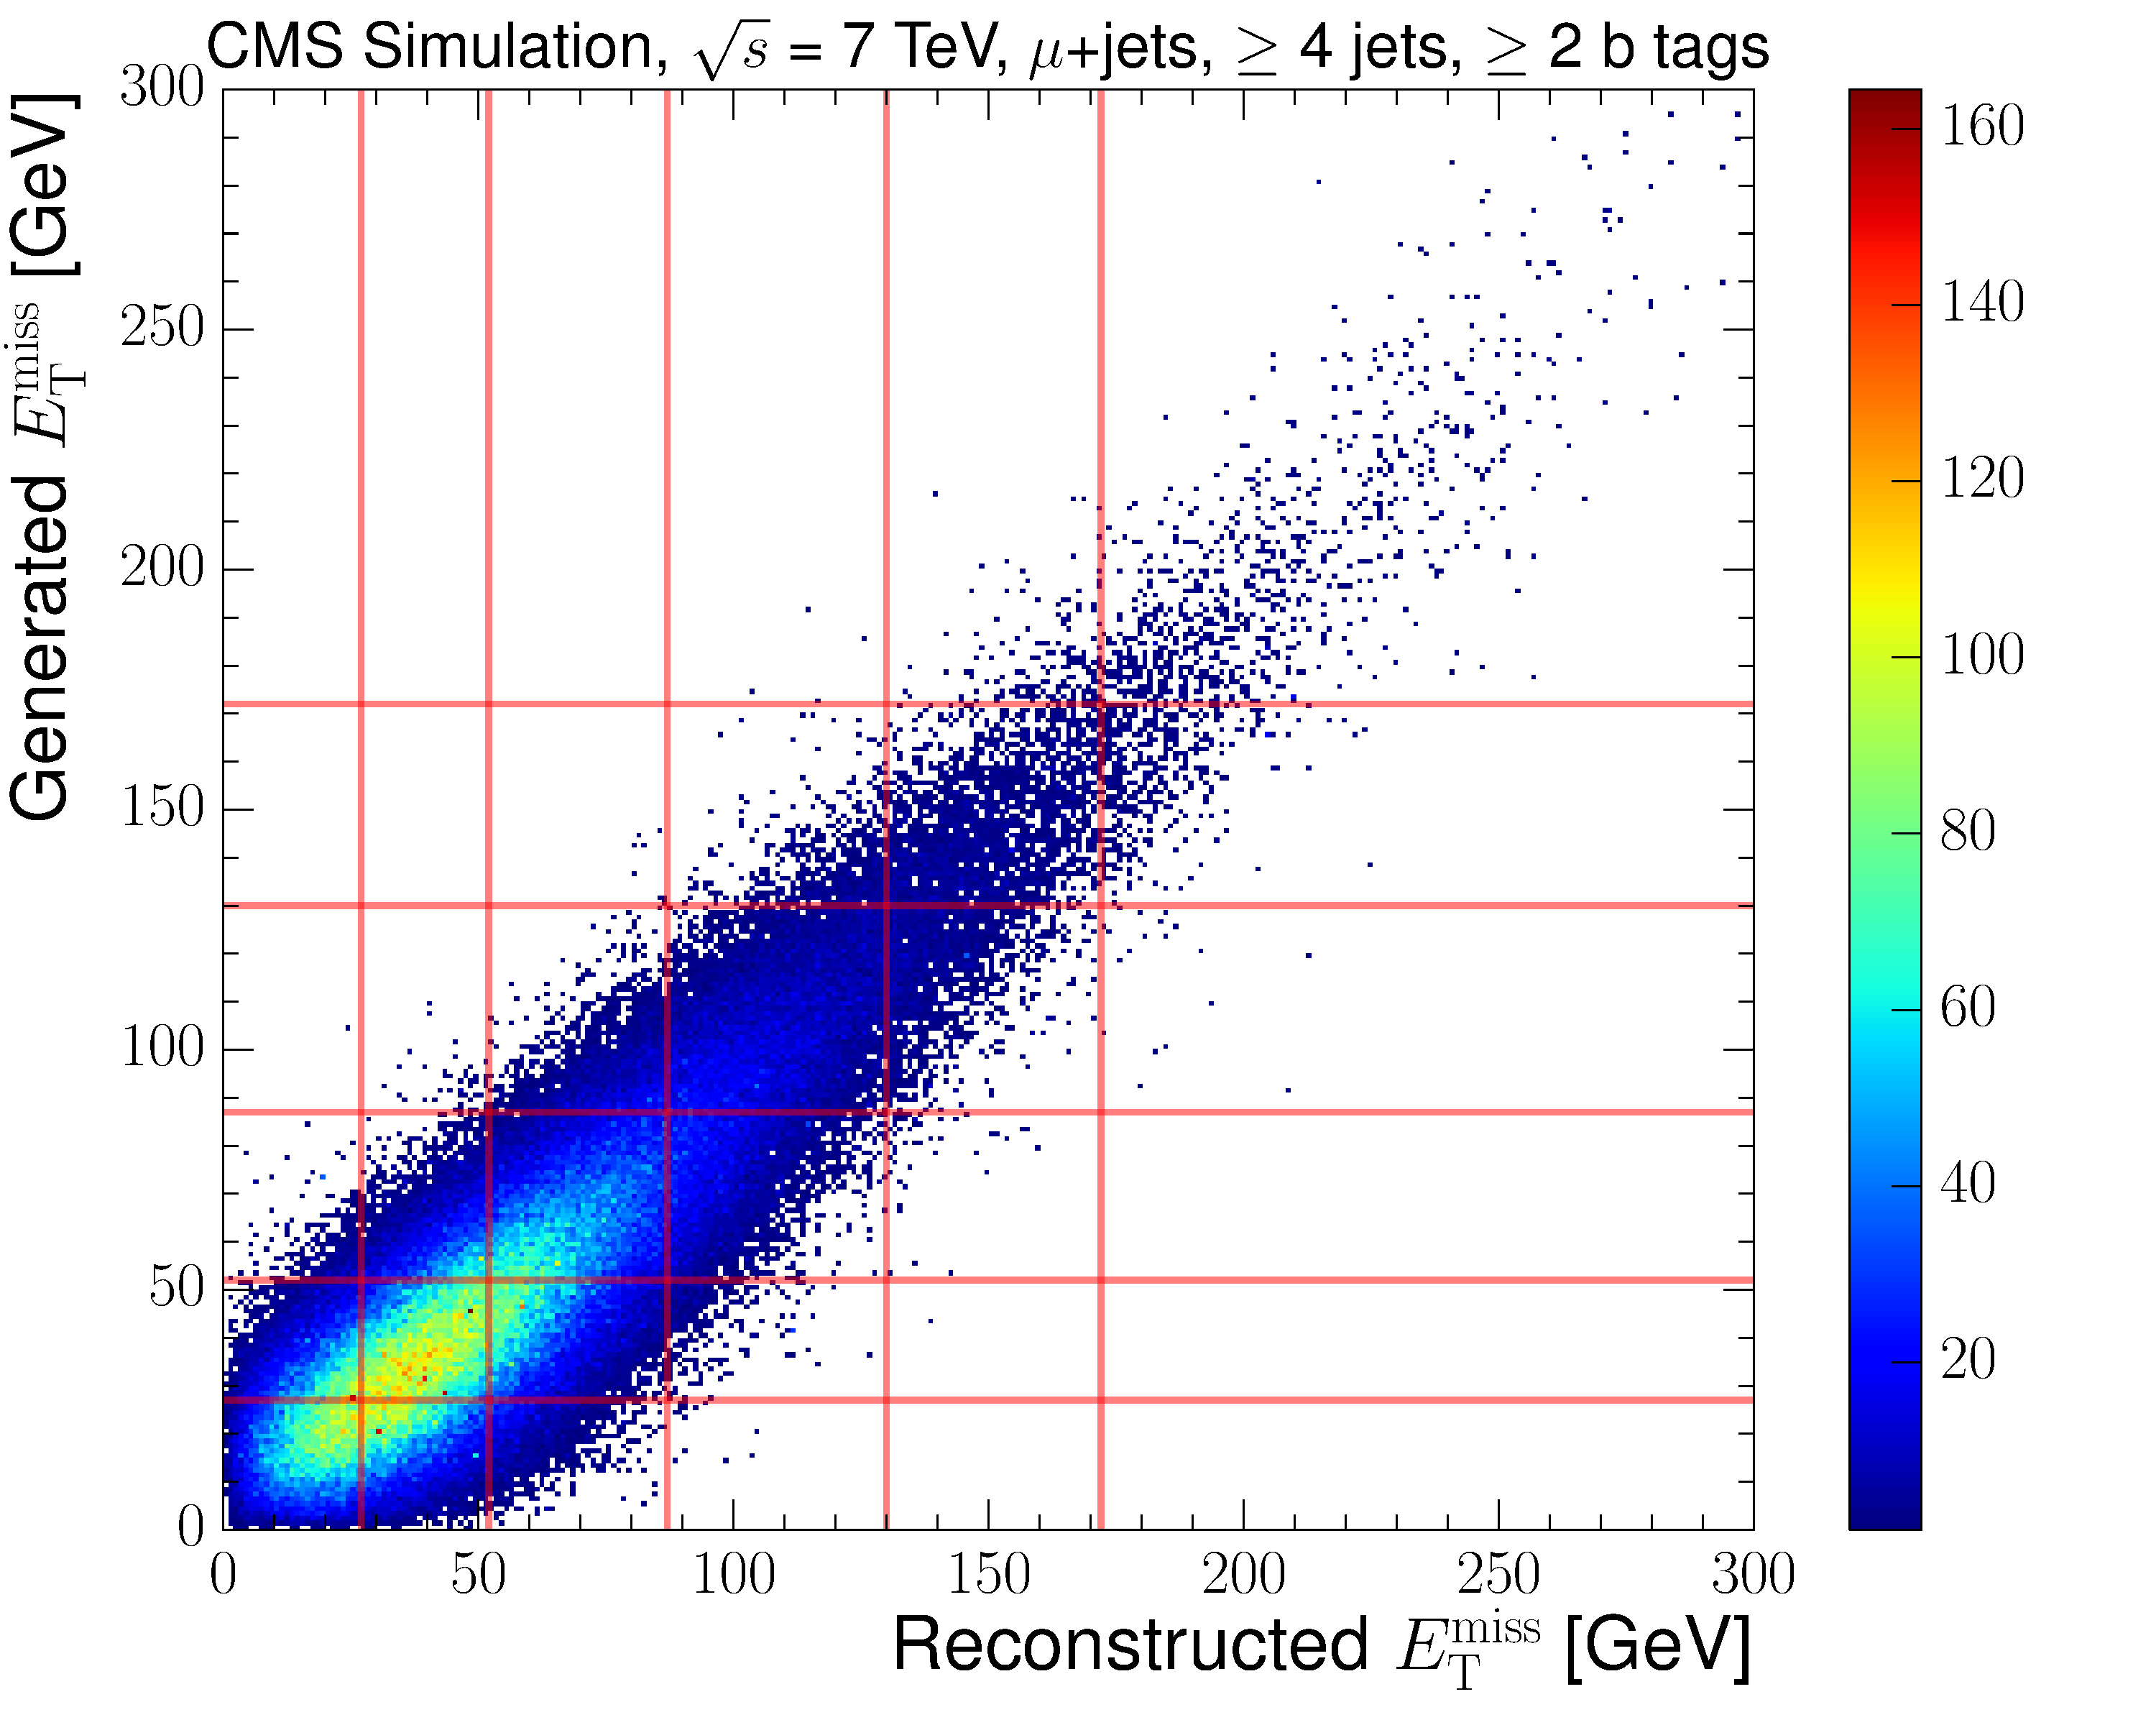
\includegraphics[width=0.48\textwidth]{Chapters/07_08_09_Analysis/Images/binning/muon_MET_7TeV.pdf}\hfill
     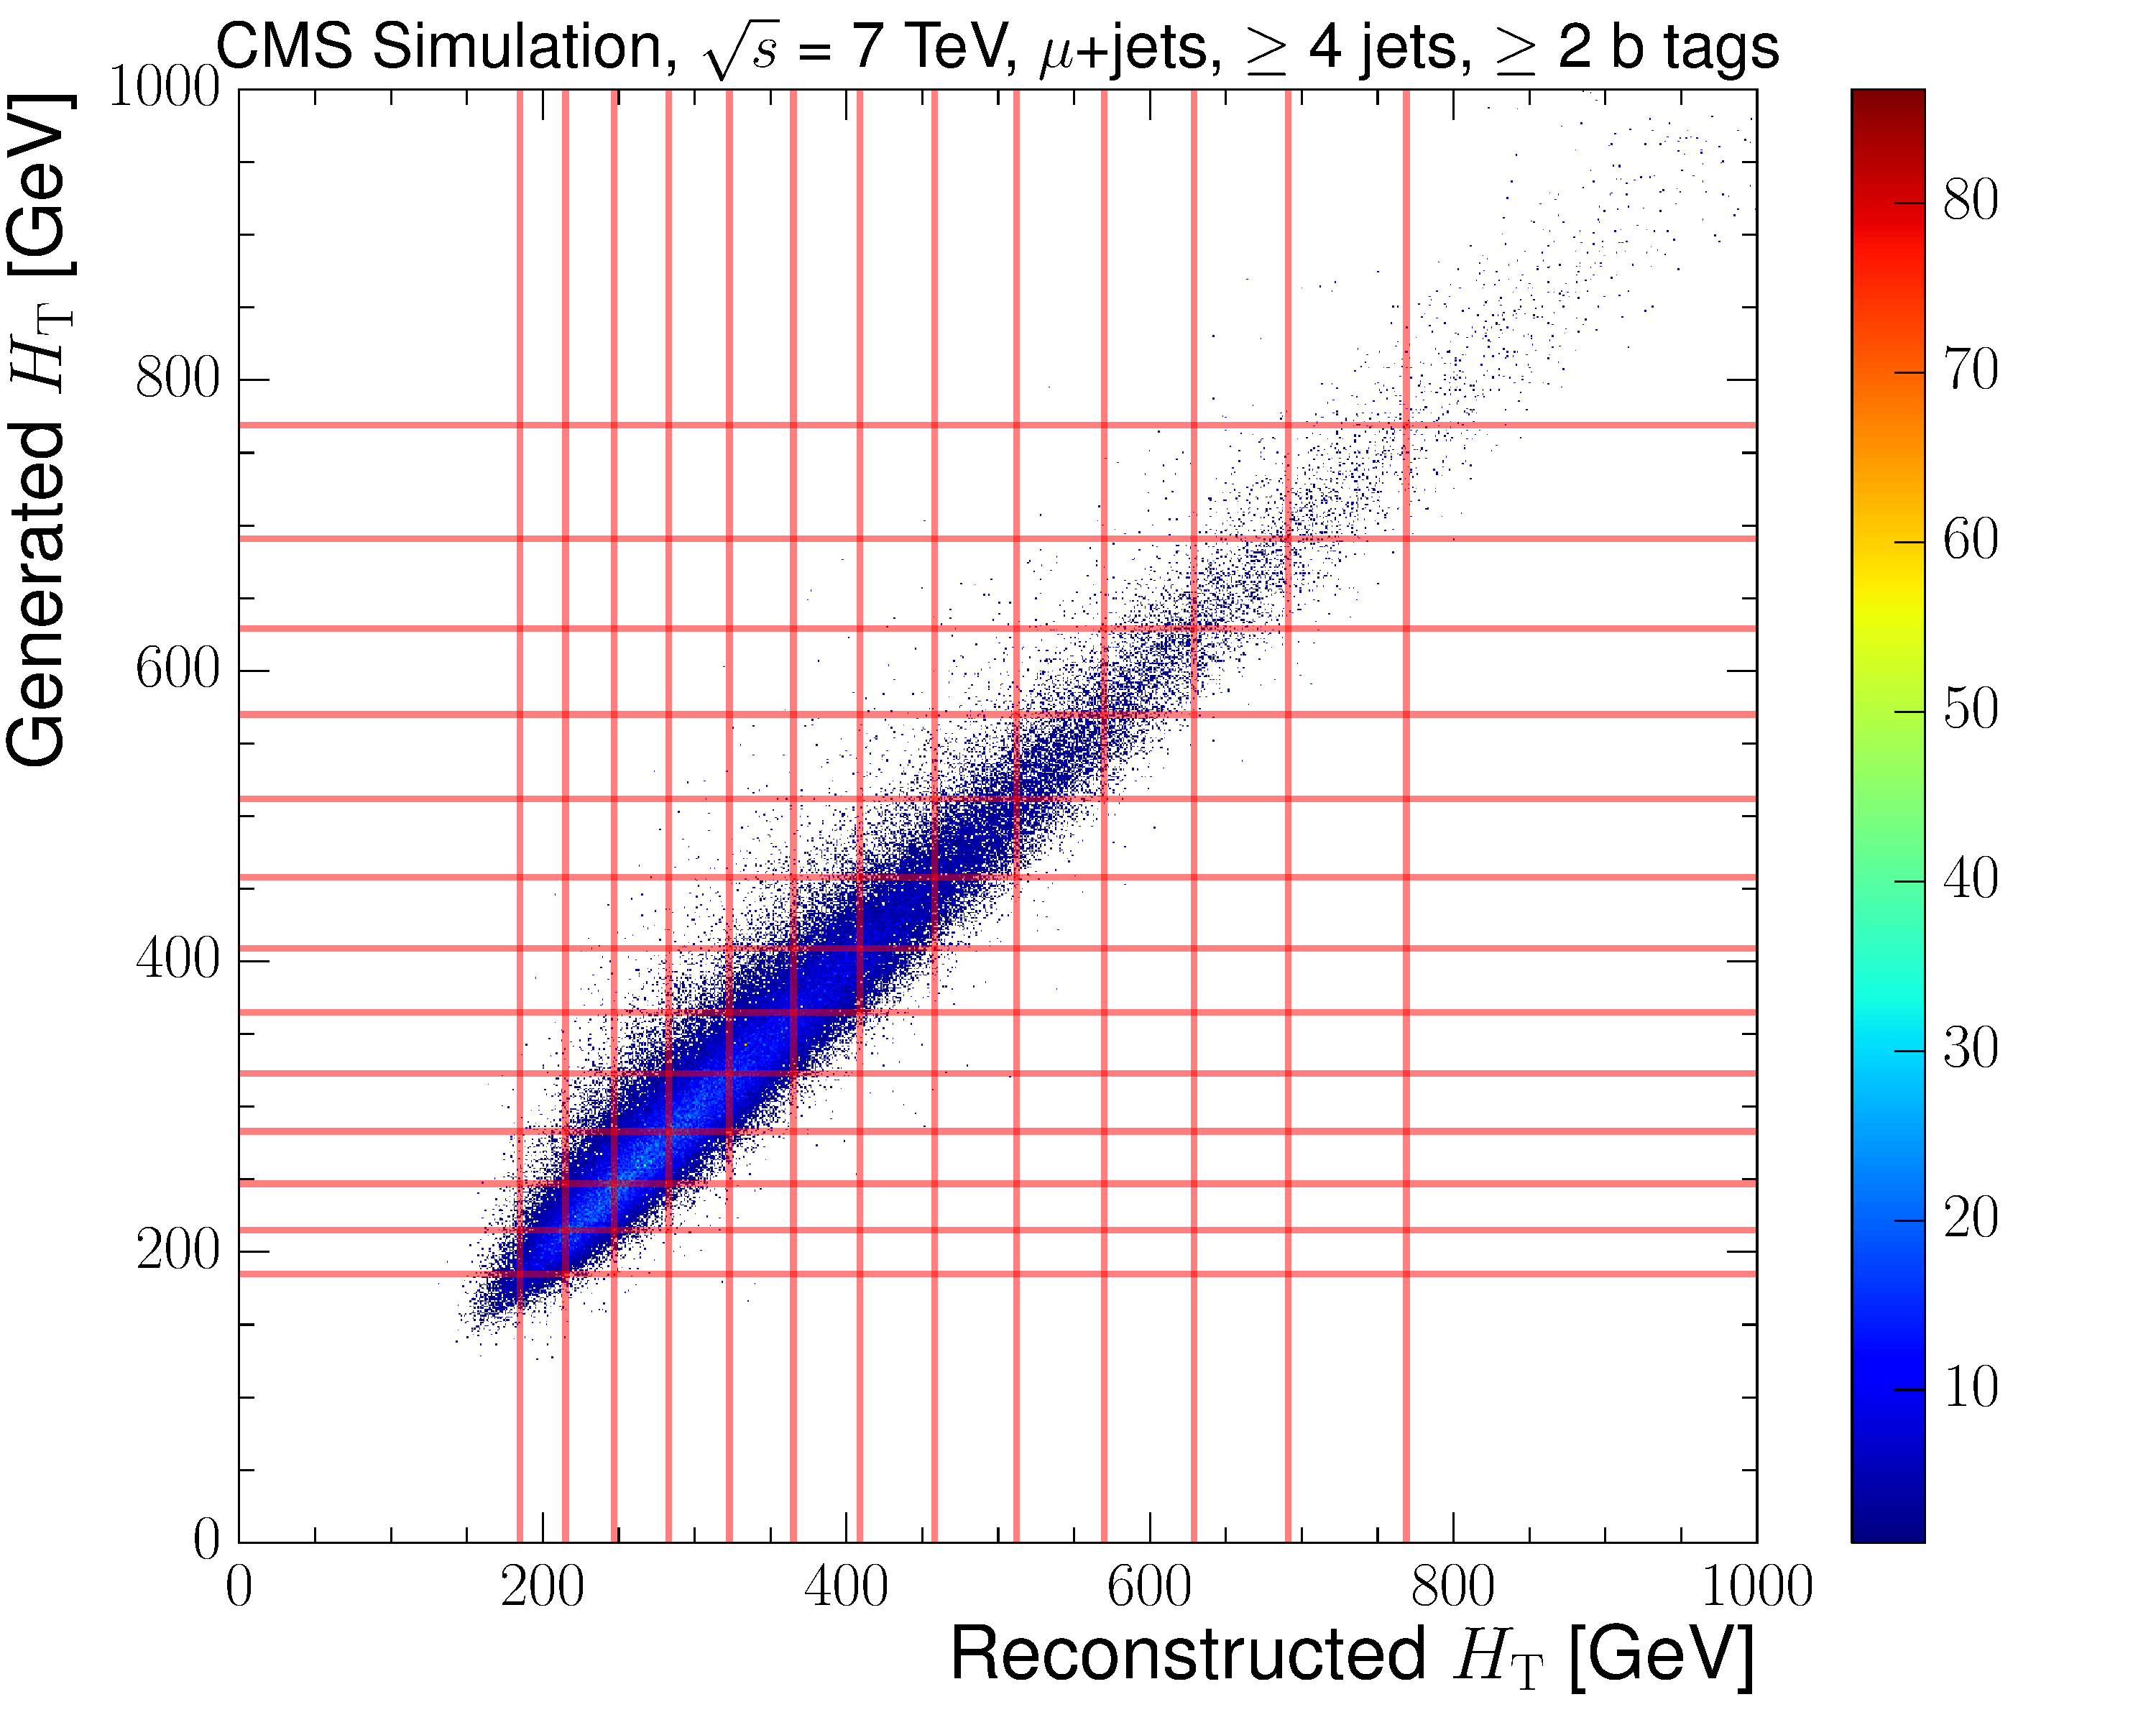
\includegraphics[width=0.48\textwidth]{Chapters/07_08_09_Analysis/Images/binning/muon_HT_7TeV.pdf}\\
     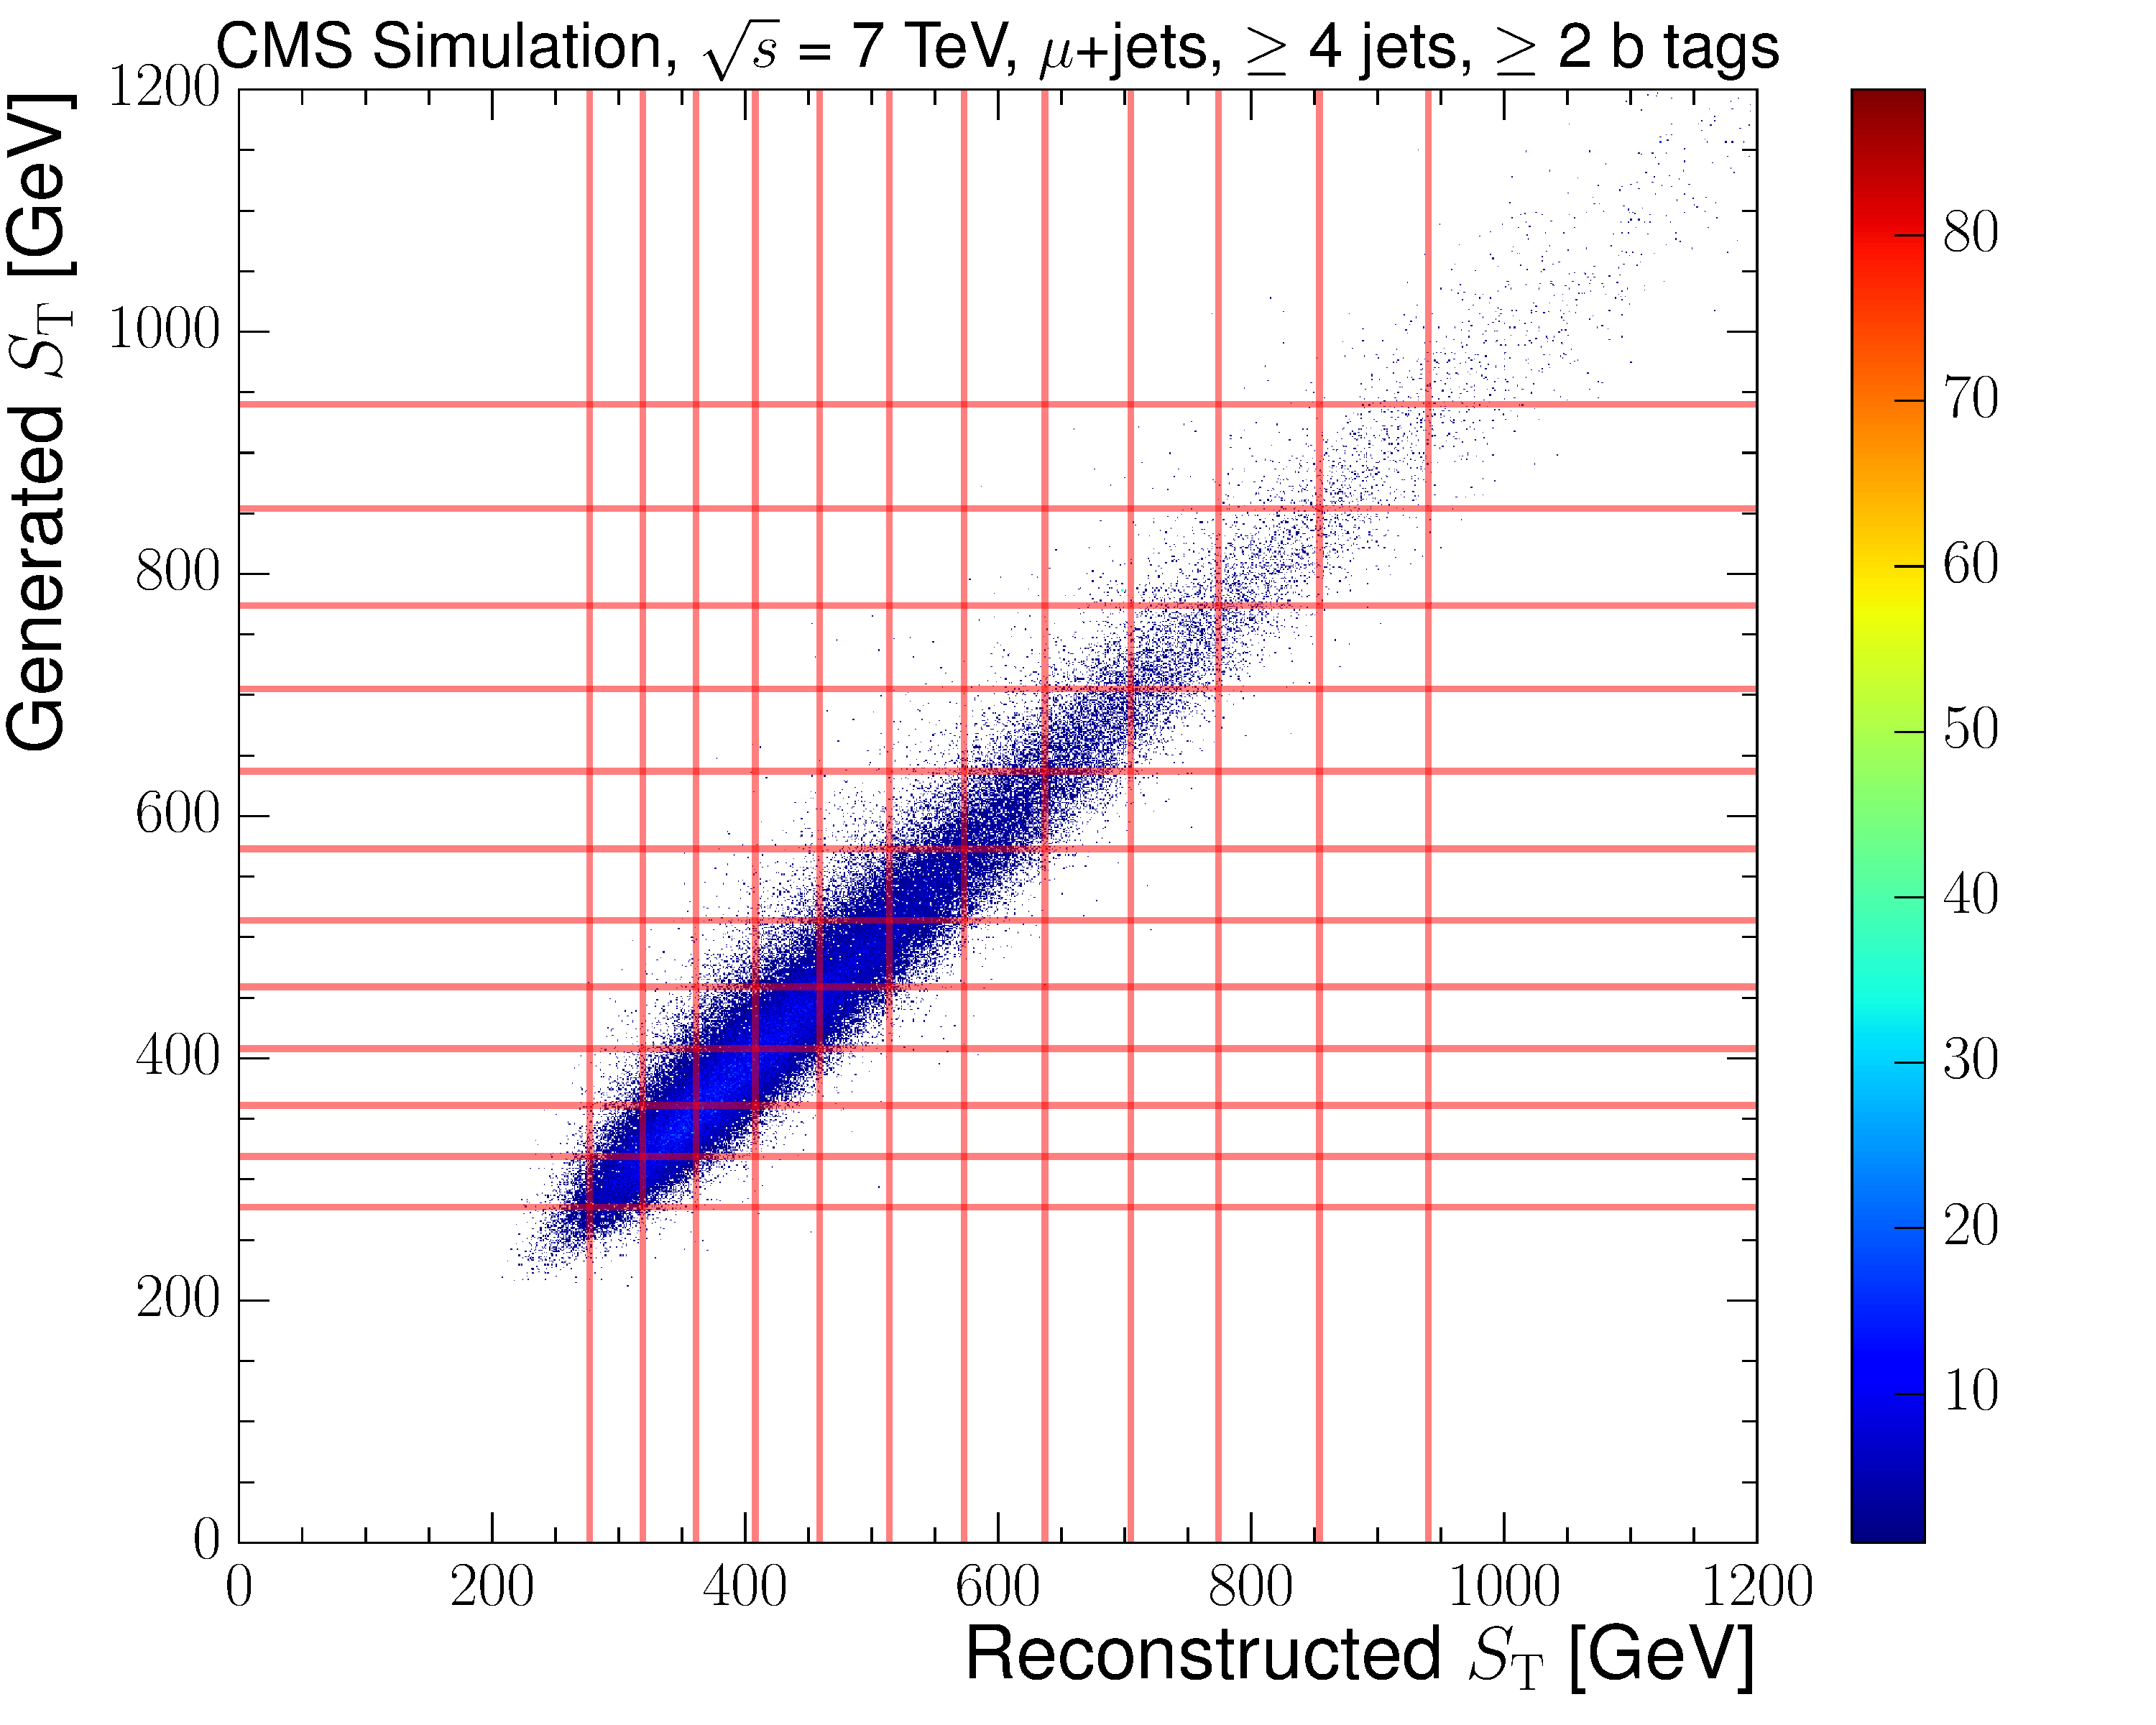
\includegraphics[width=0.48\textwidth]{Chapters/07_08_09_Analysis/Images/binning/muon_ST_7TeV.pdf}\hfill
     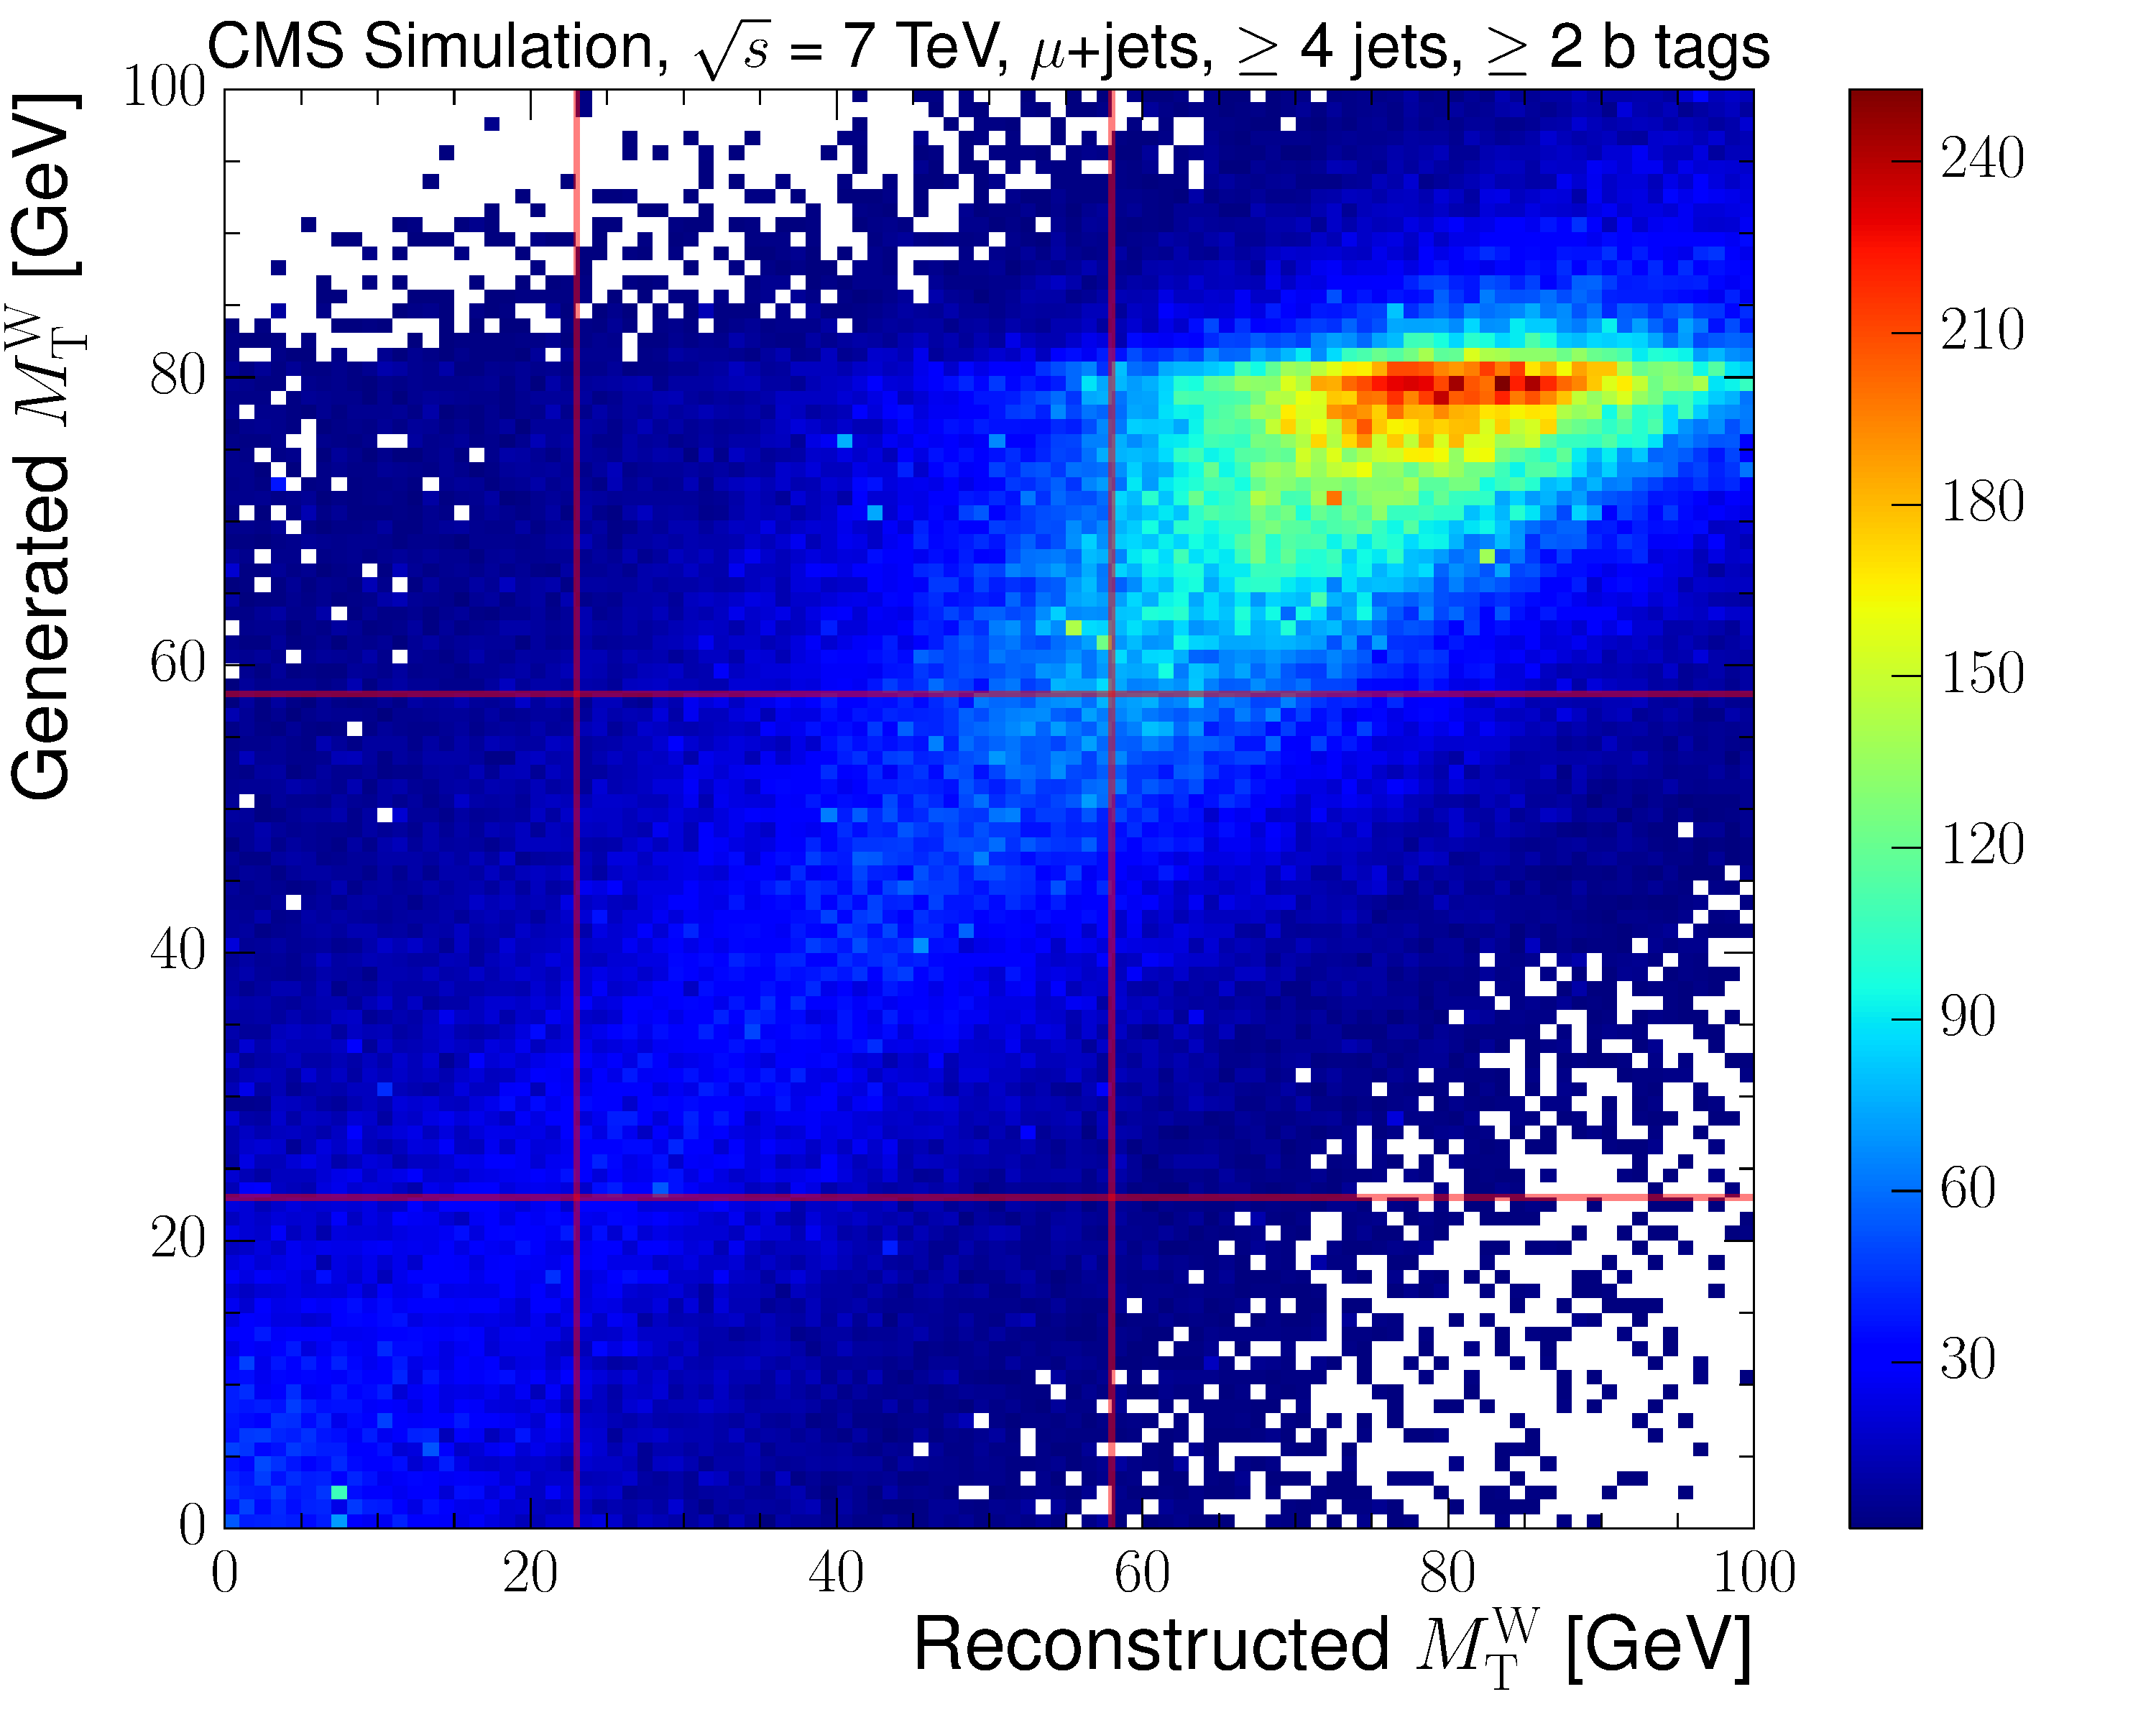
\includegraphics[width=0.48\textwidth]{Chapters/07_08_09_Analysis/Images/binning/muon_MT_7TeV.pdf}\\
	 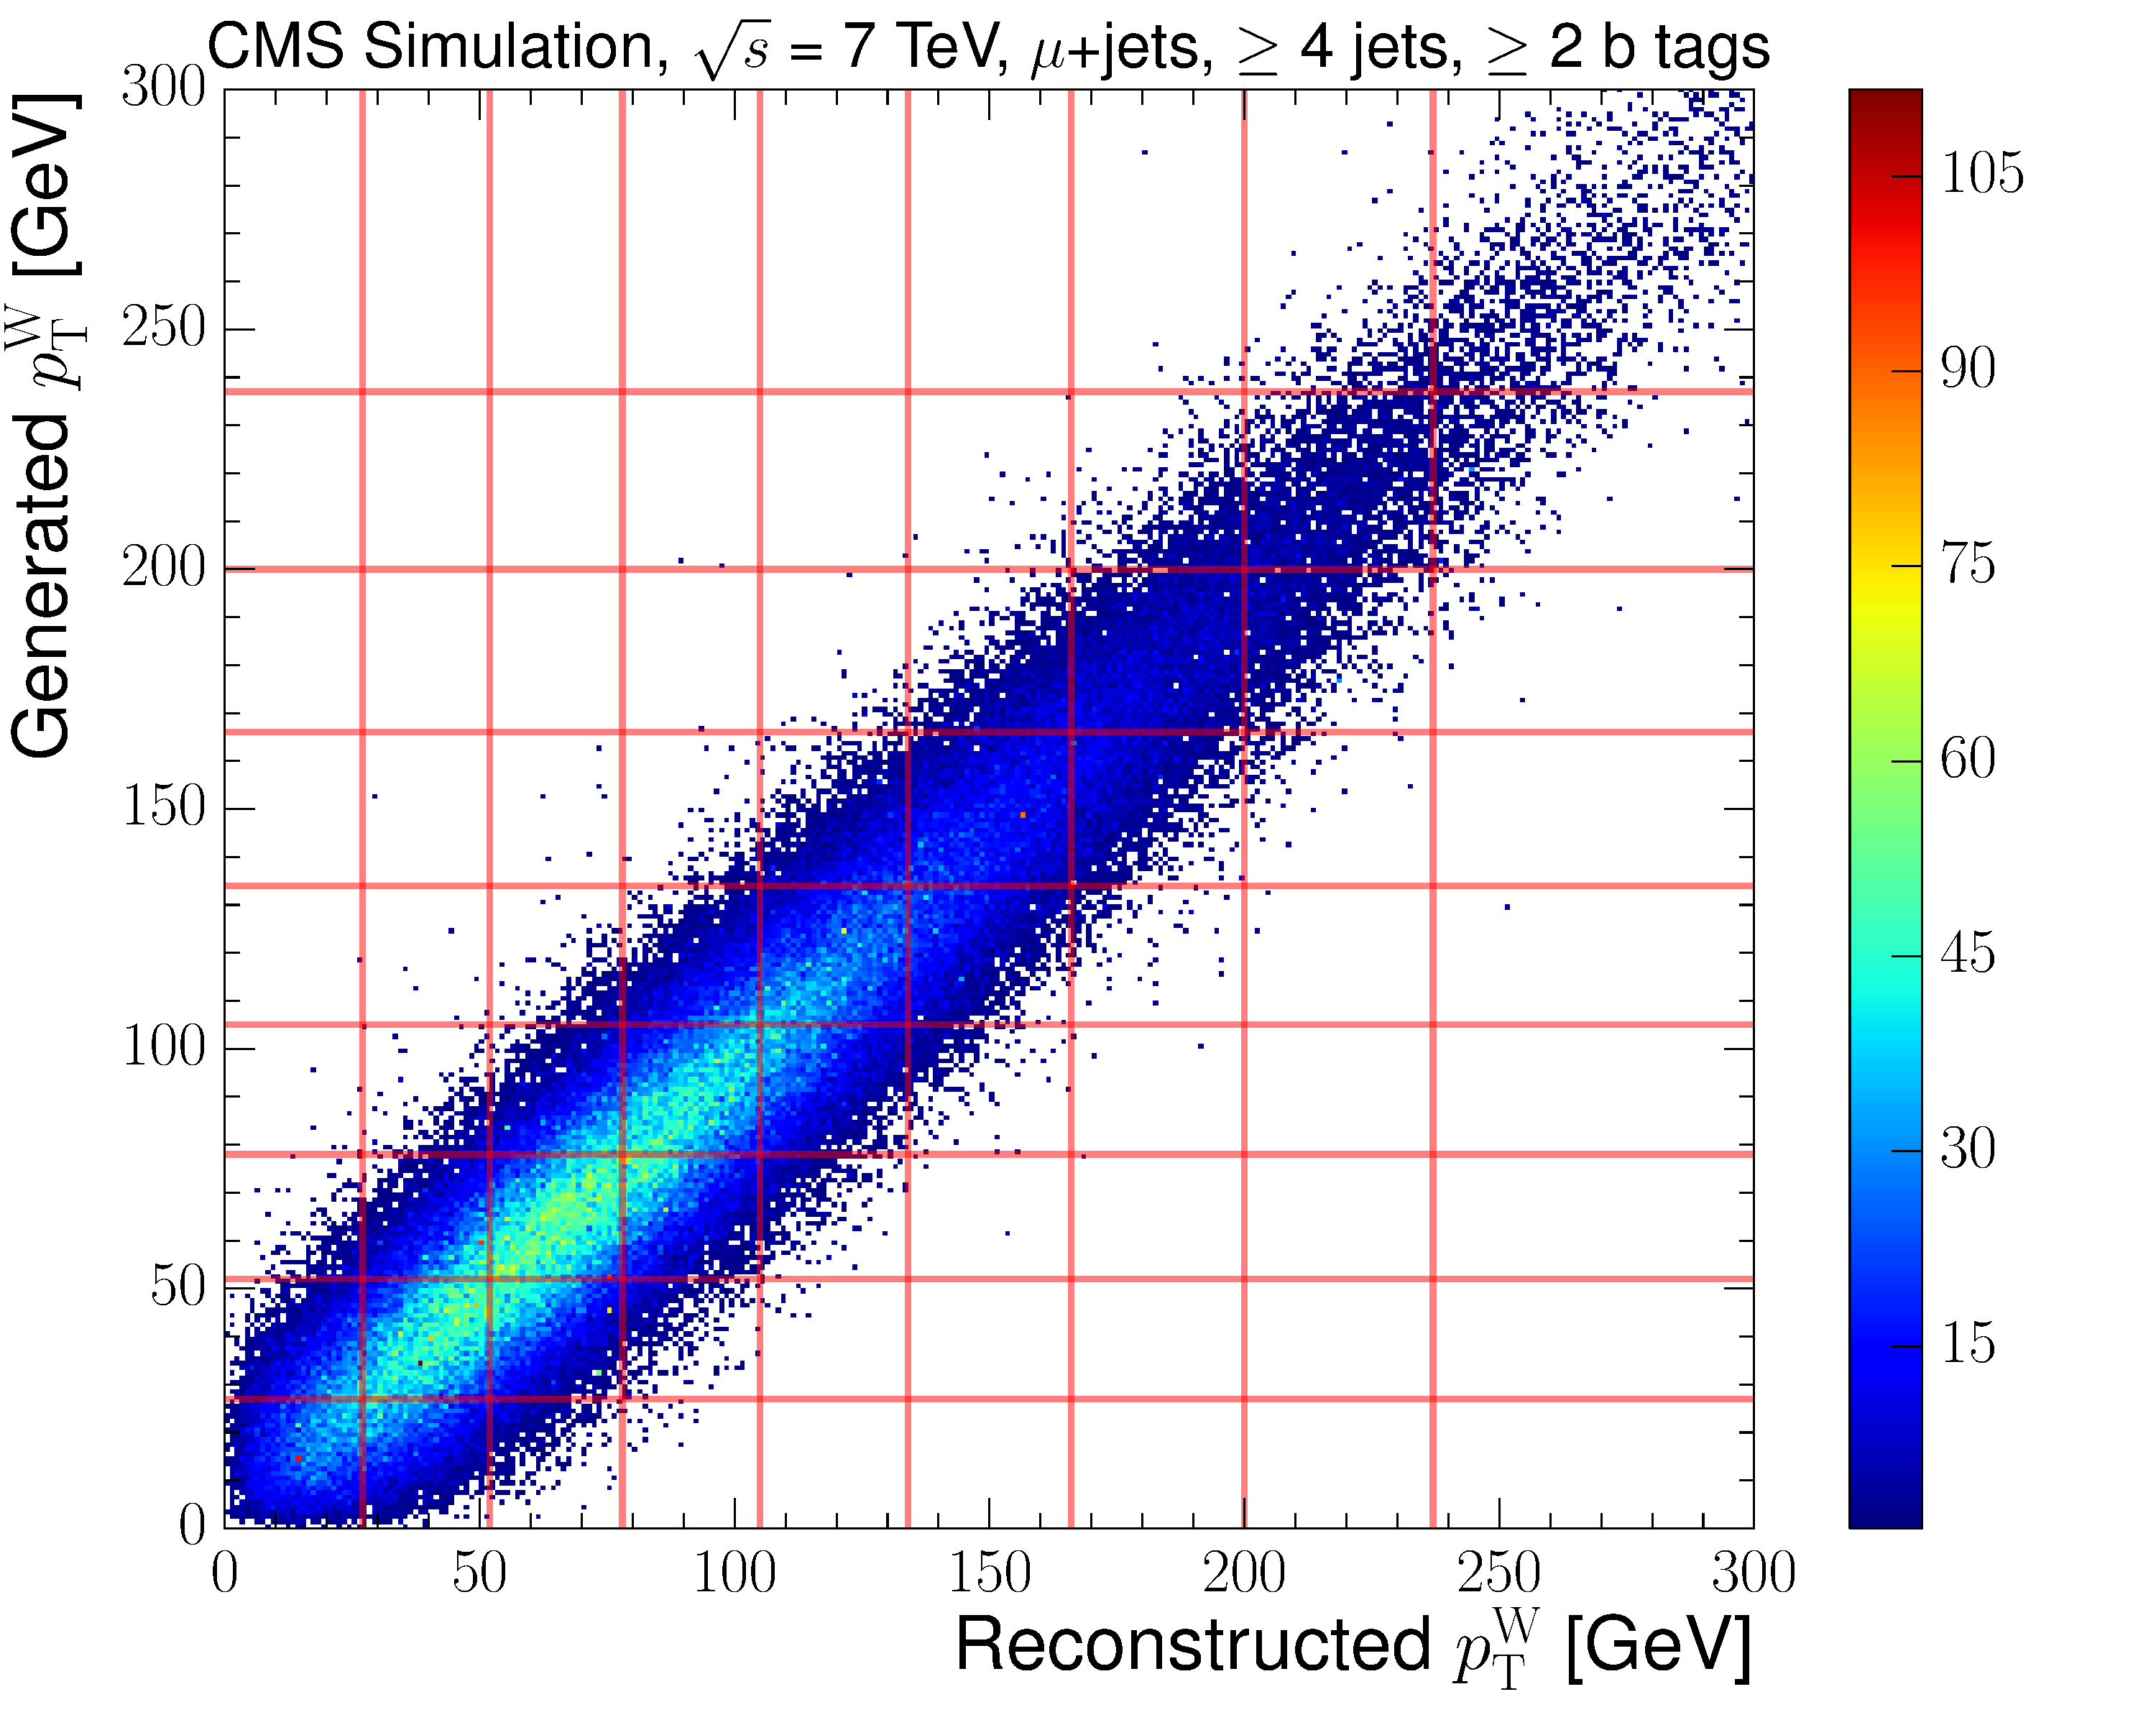
\includegraphics[width=0.48\textwidth]{Chapters/07_08_09_Analysis/Images/binning/muon_WPT_7TeV.pdf}\hfill
	 \caption[Generated versus reconstructed distributions of the primary variables at $\sqrt{s}=7\TeV$ in the
	 muon+jets channel.]{Generated versus reconstructed distributions of the primary variables \met (upper left),
	 \HT (upper right), \st (middle left), \mt (middle right) and \wpt (lower) with horizontal and vertical lines
	 representing the boundaries of the selected bins at $\sqrt{s}=7\TeV$ in the muon+jets channel. These
	 distributions are obtained using \ttbar simulation.}
     \label{fig:binning_7TeV_muon}
 \end{figure}

 \begin{figure}[H]
    \centering
     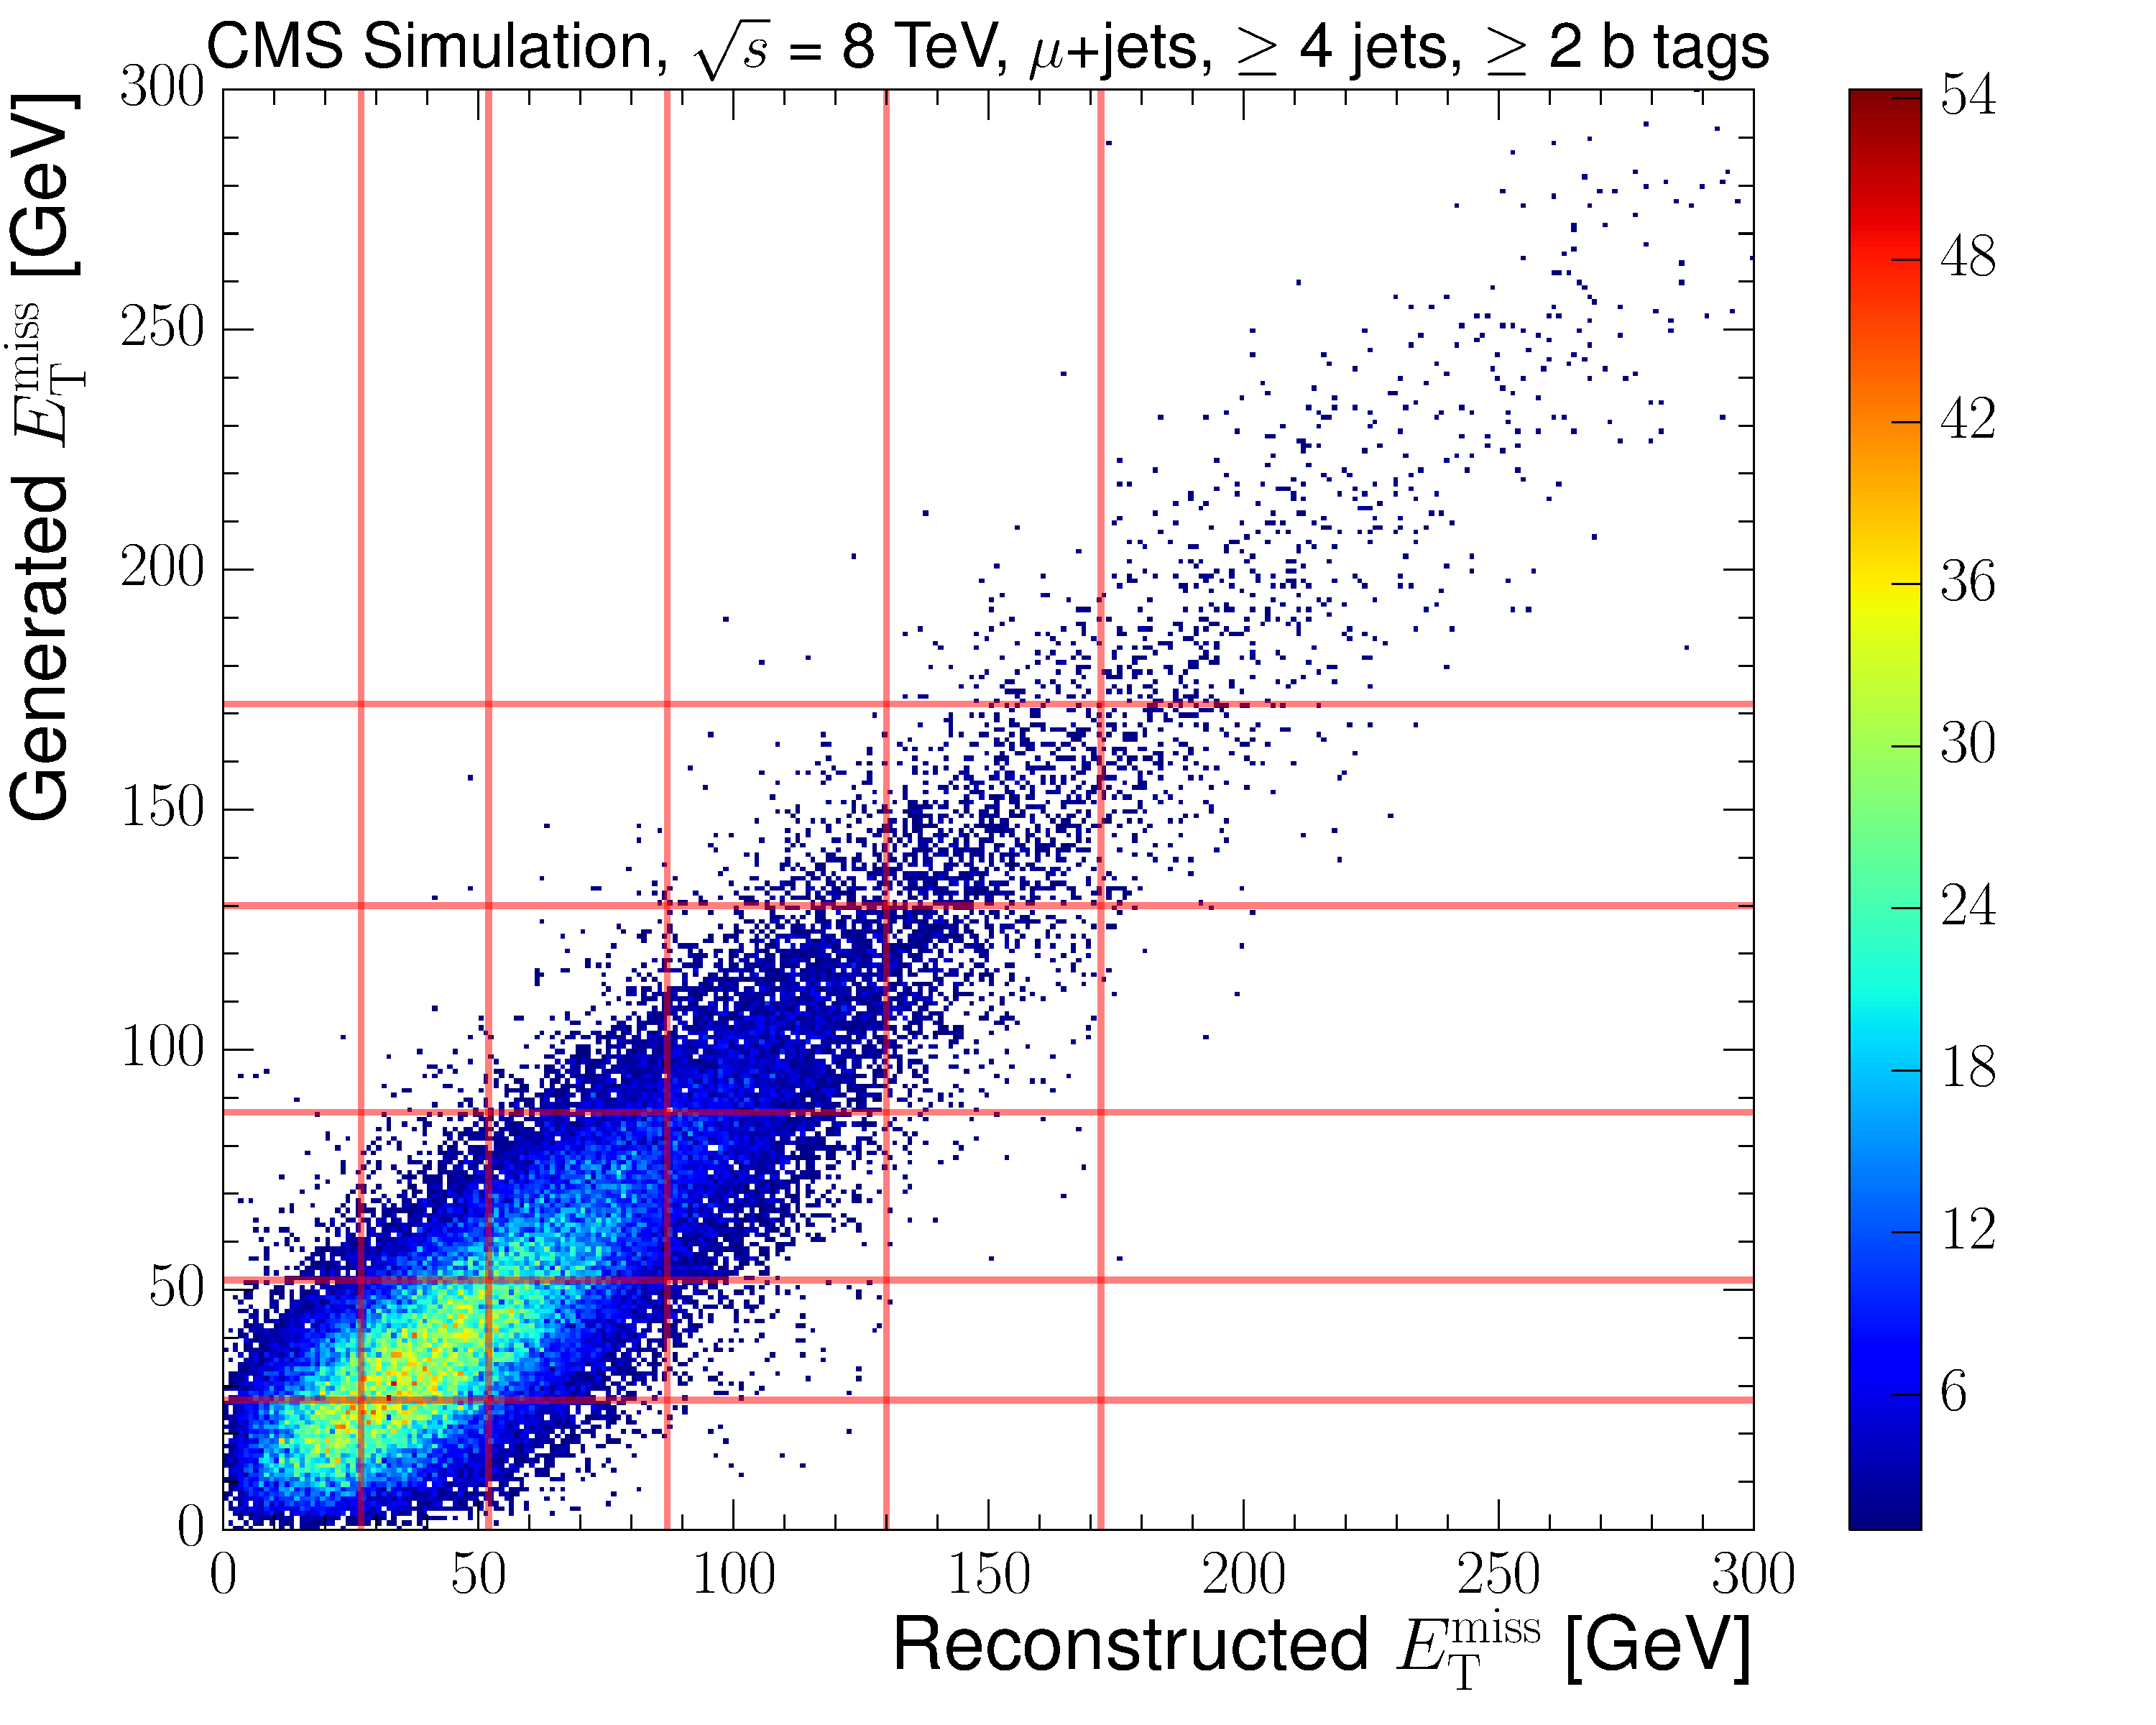
\includegraphics[width=0.48\textwidth]{Chapters/07_08_09_Analysis/Images/binning/muon_MET_8TeV.pdf}\hfill
     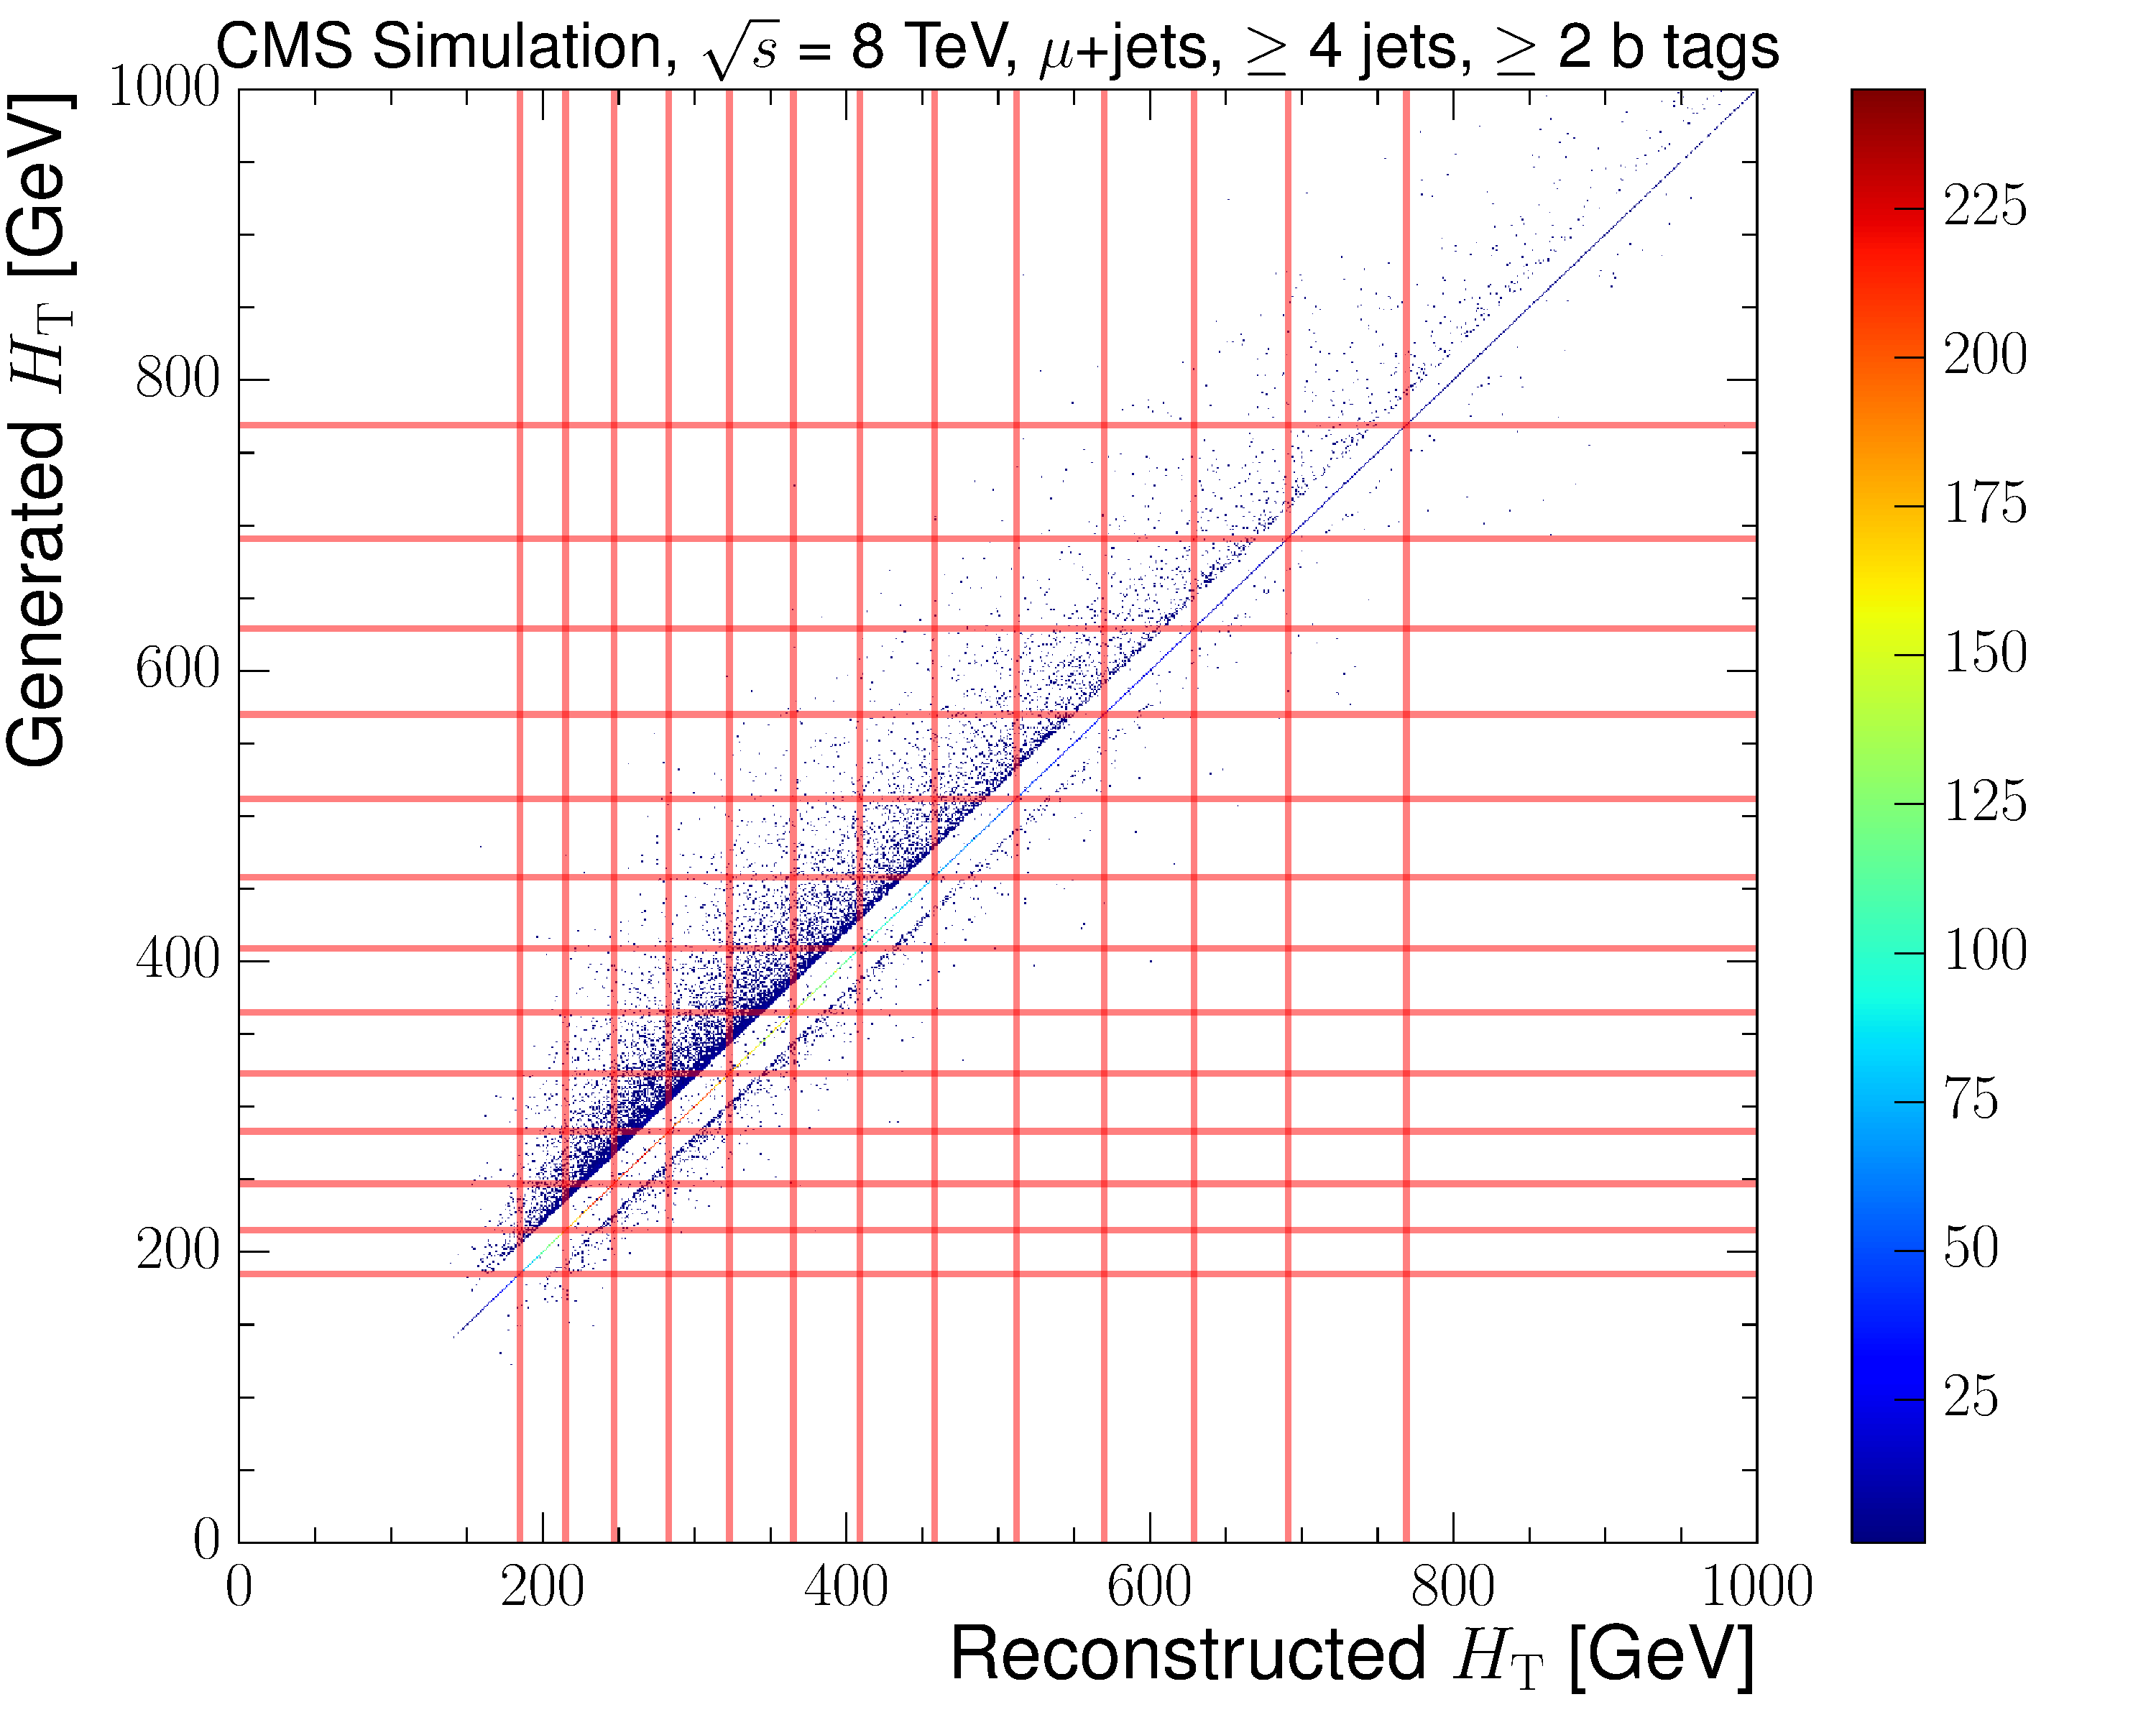
\includegraphics[width=0.48\textwidth]{Chapters/07_08_09_Analysis/Images/binning/muon_HT_8TeV.pdf}\\
     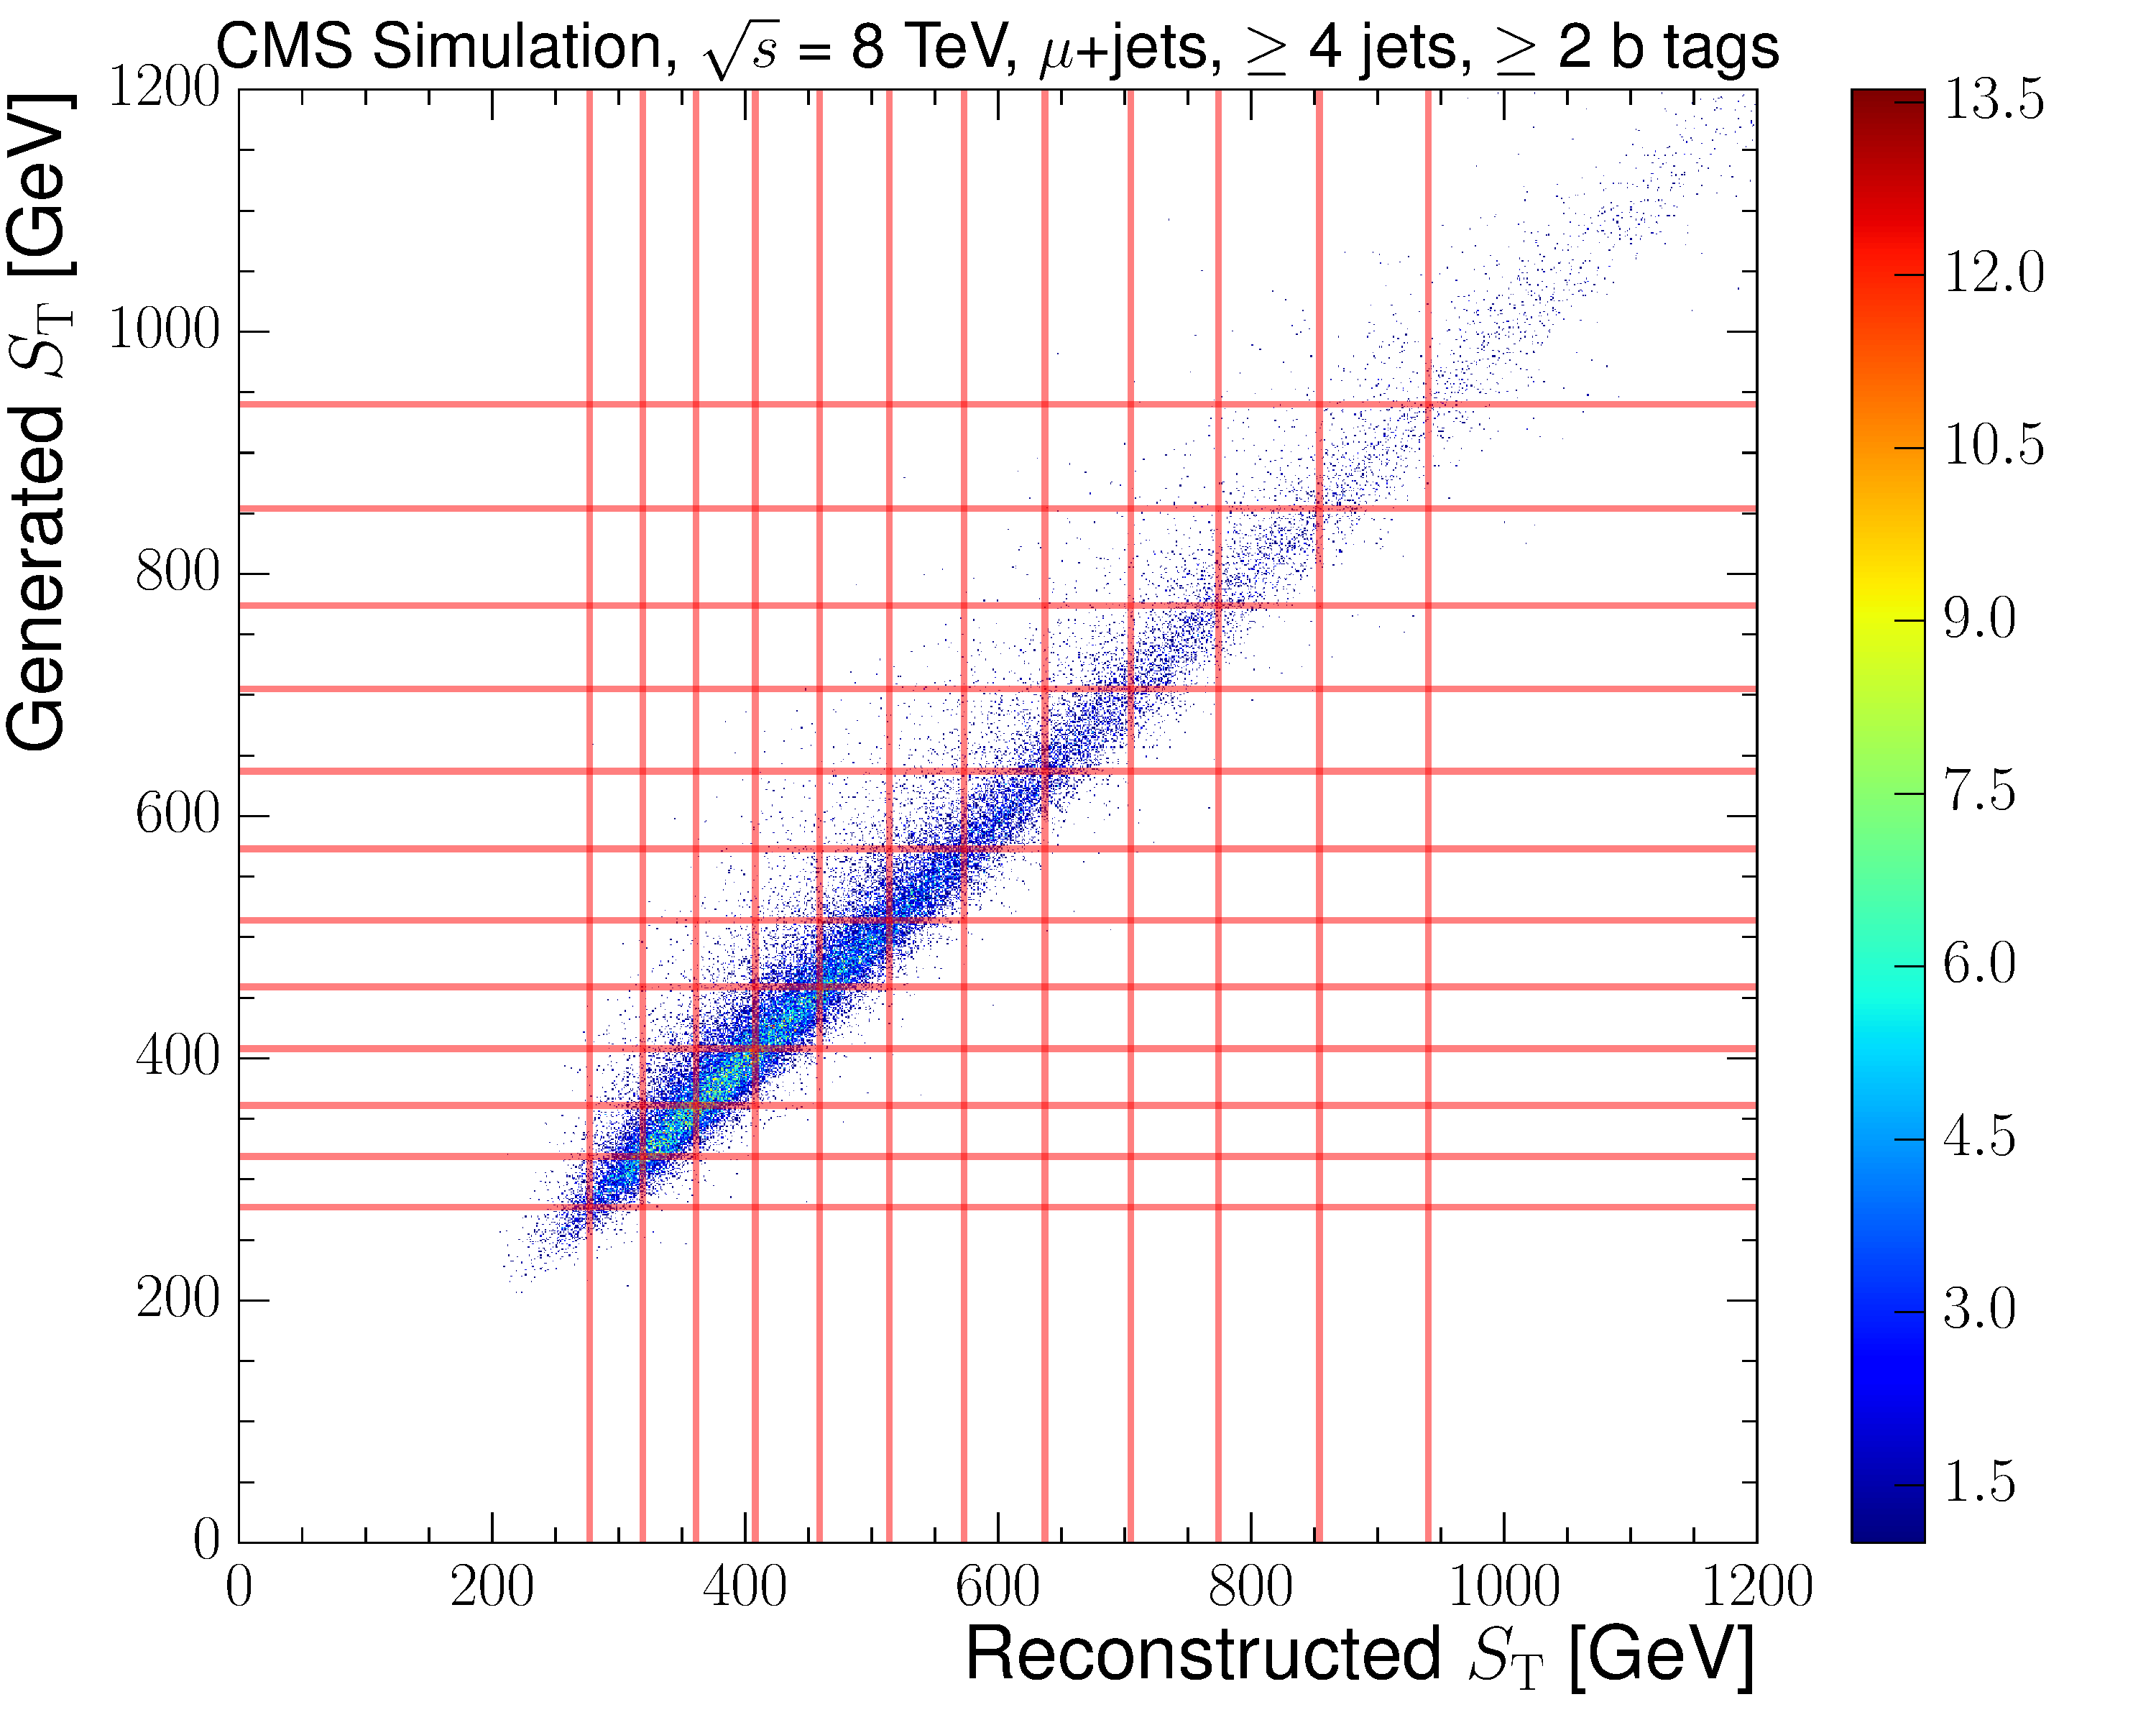
\includegraphics[width=0.48\textwidth]{Chapters/07_08_09_Analysis/Images/binning/muon_ST_8TeV.pdf}\hfill
     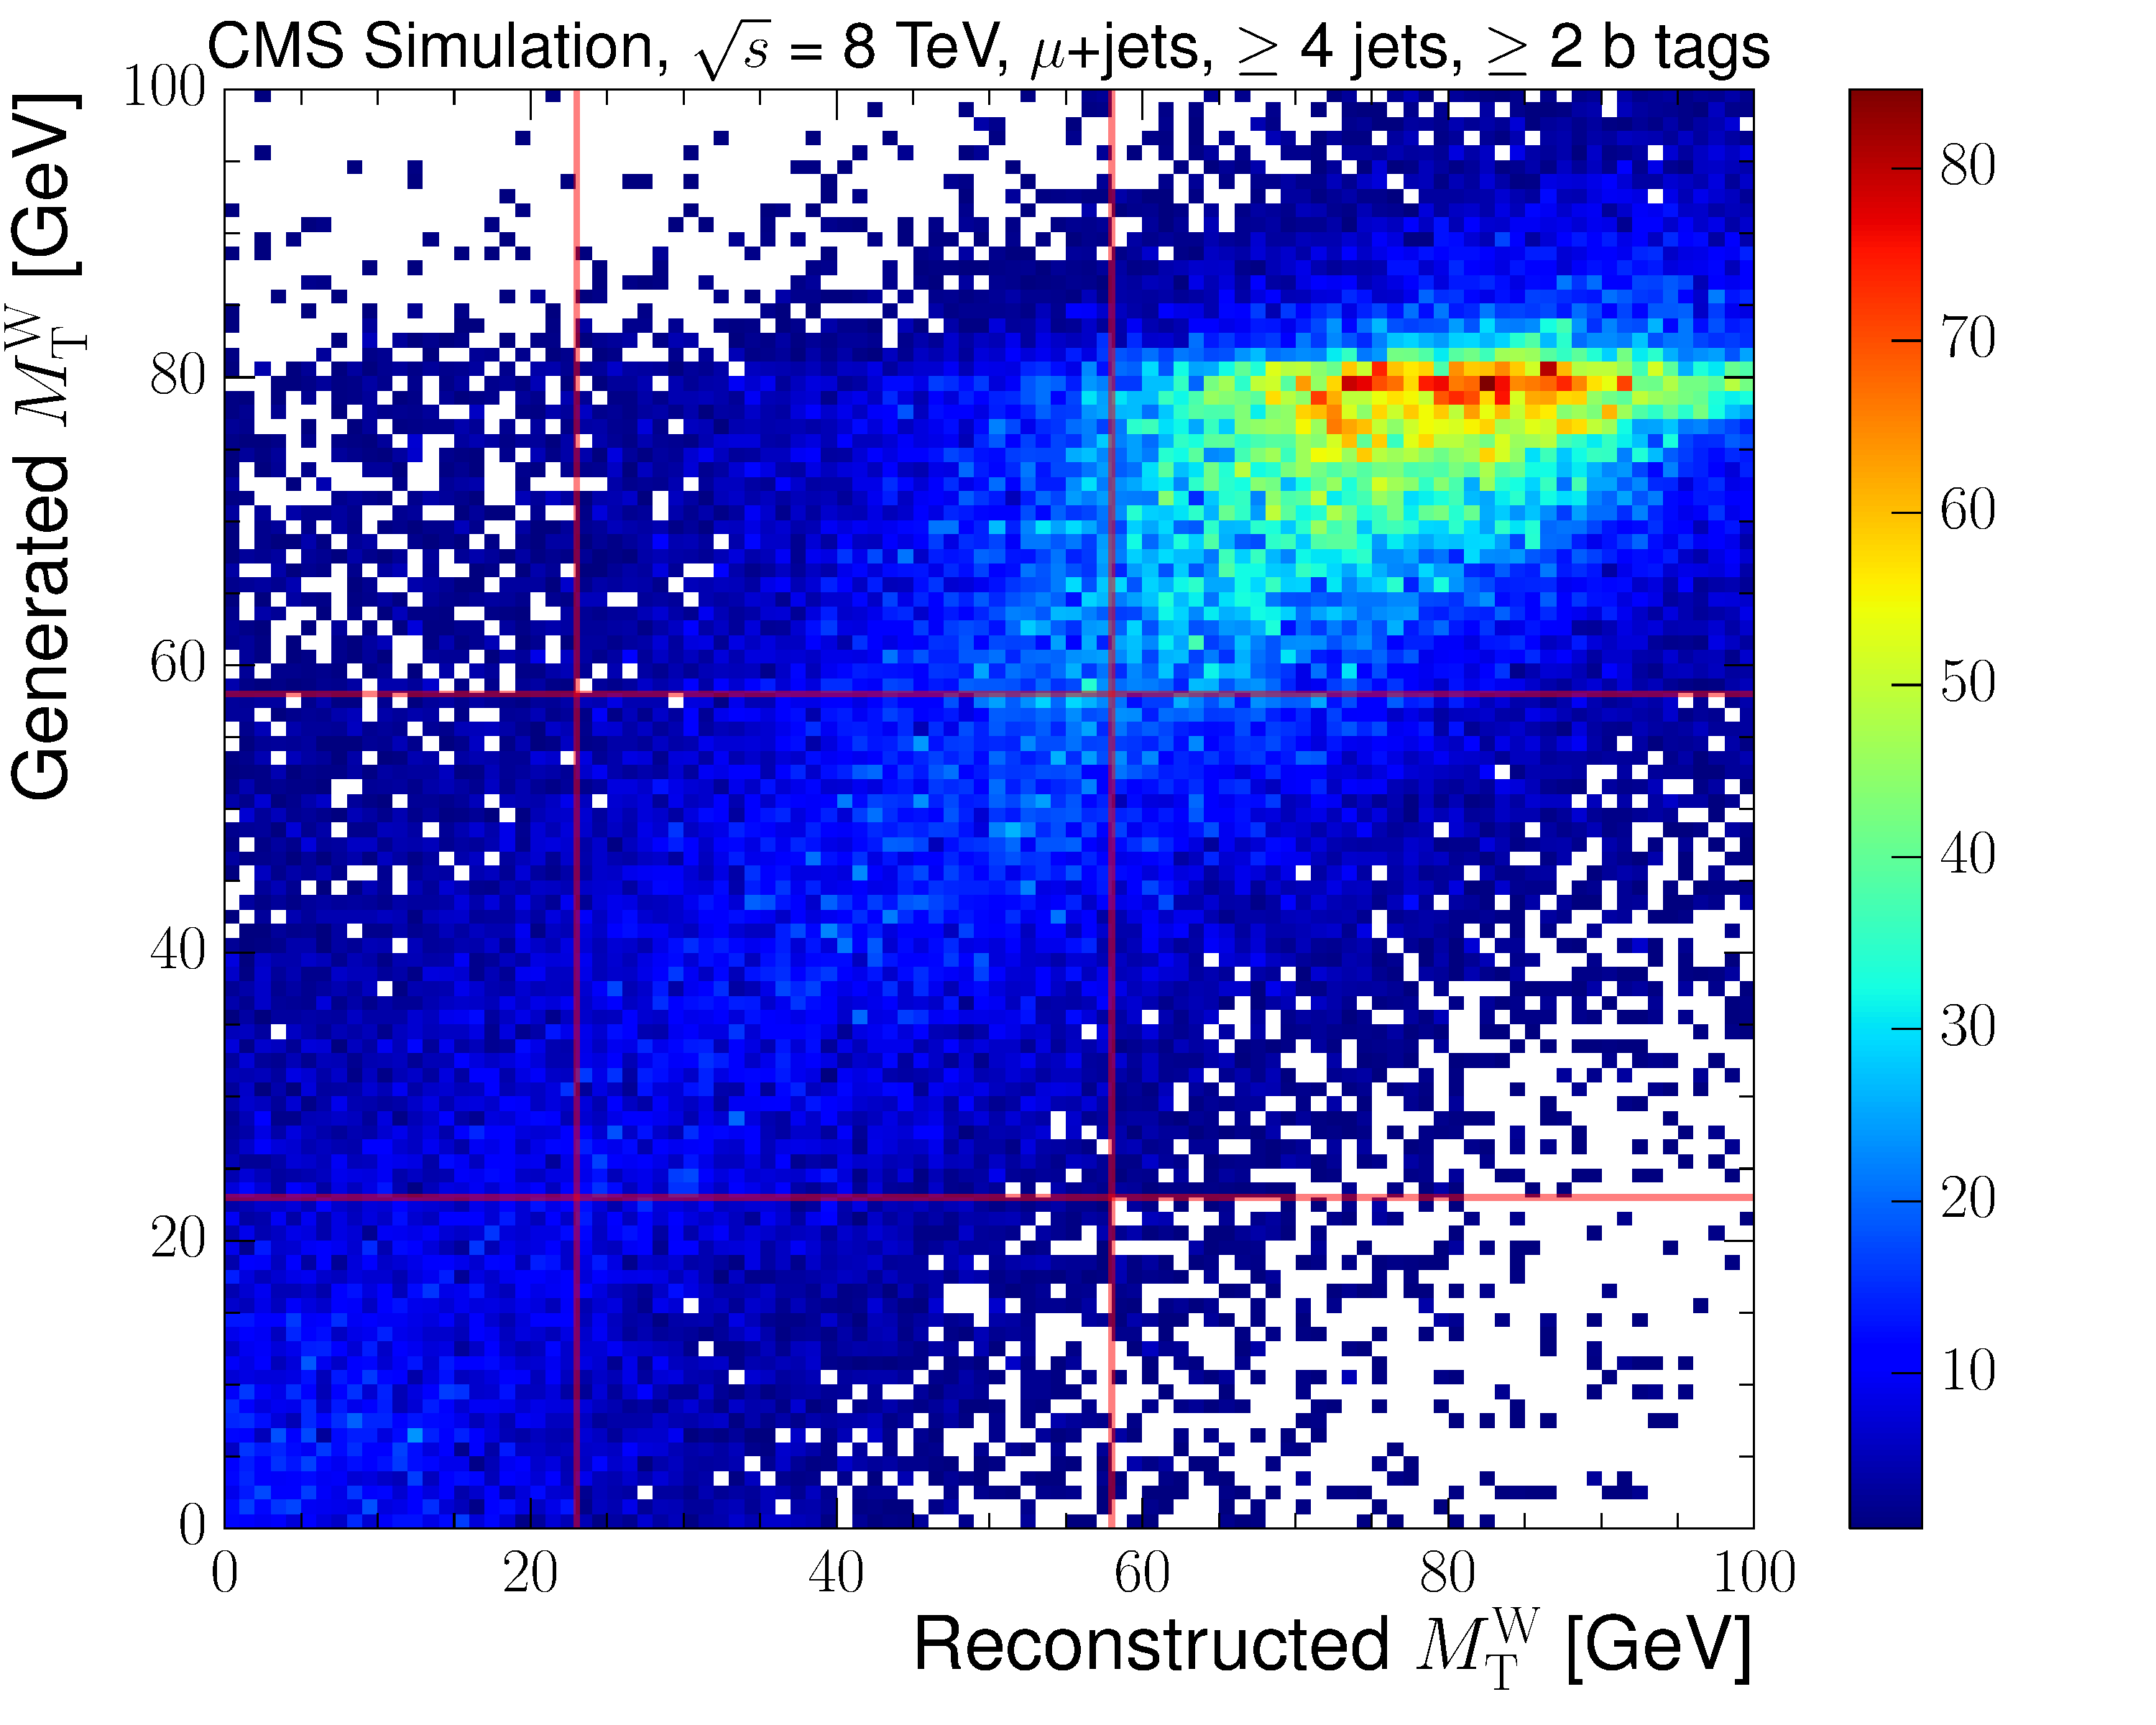
\includegraphics[width=0.48\textwidth]{Chapters/07_08_09_Analysis/Images/binning/muon_MT_8TeV.pdf}\\
	 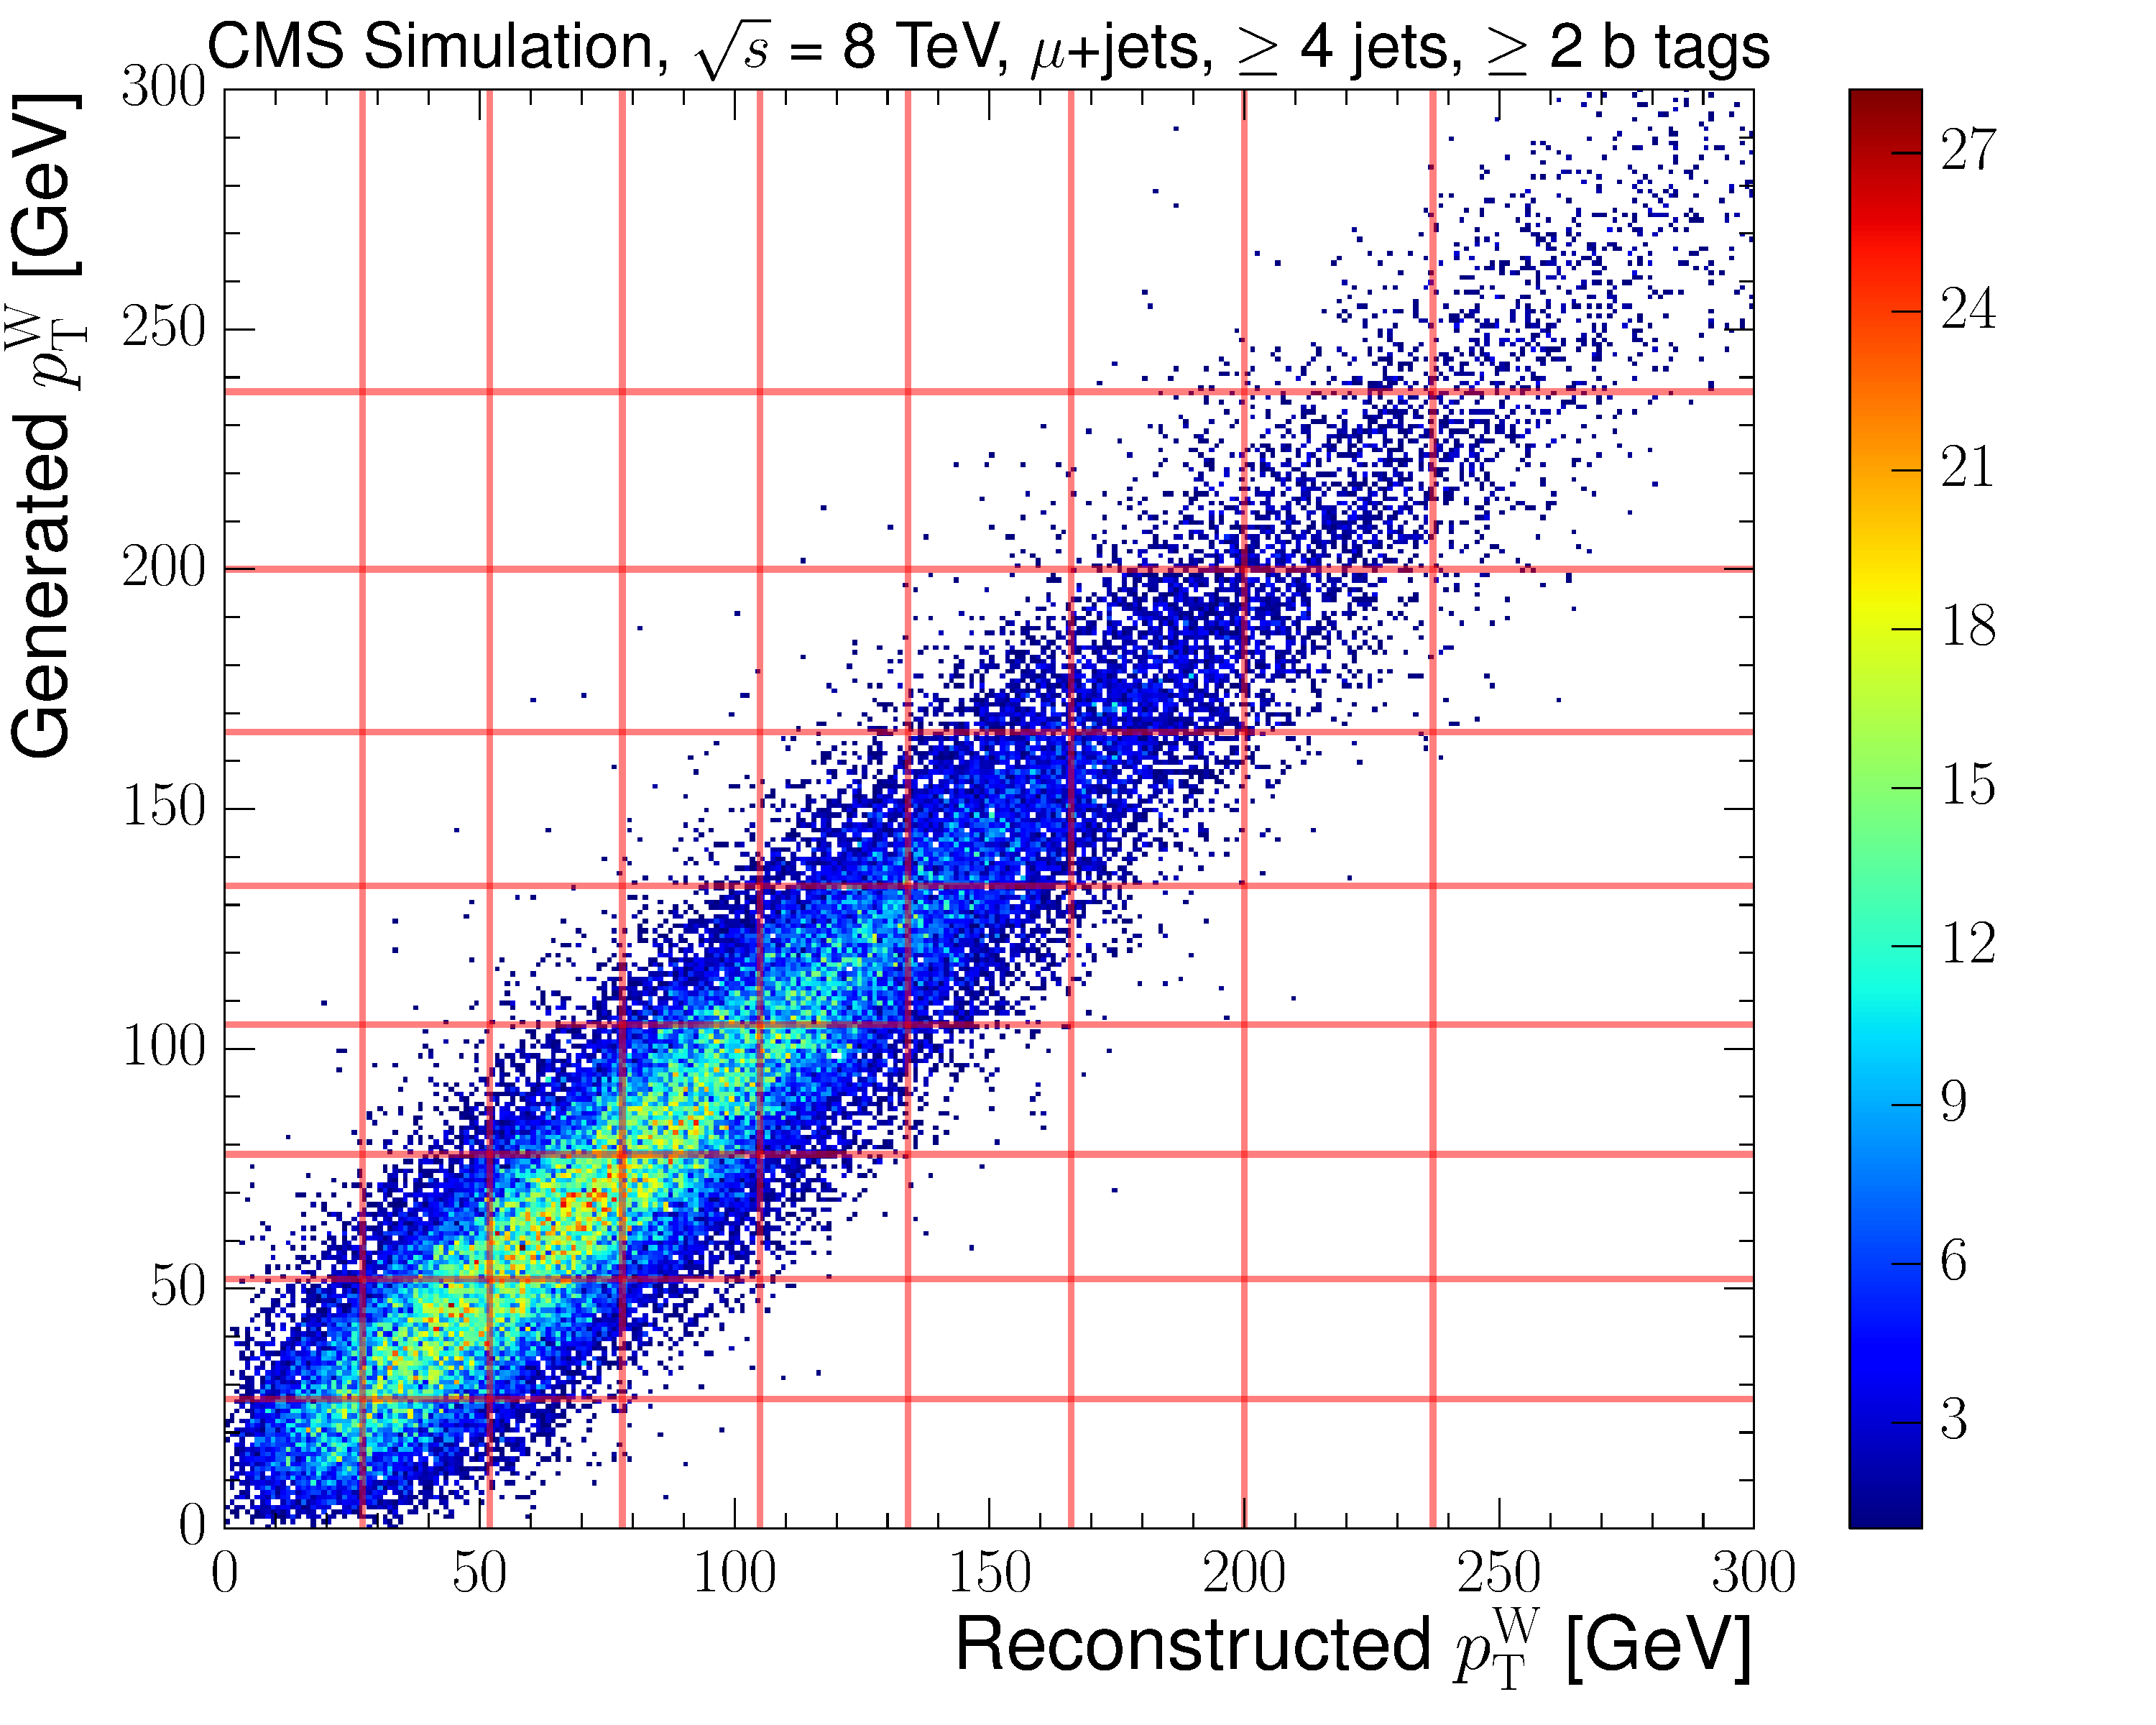
\includegraphics[width=0.48\textwidth]{Chapters/07_08_09_Analysis/Images/binning/muon_WPT_8TeV.pdf}\hfill
	 \caption[Generated versus reconstructed distributions of the primary variables at $\sqrt{s}=8\TeV$ in the
	 muon+jets channel.]{Generated versus reconstructed distributions of the primary variables \met (upper left),
	 \HT (upper right), \st (middle left), \mt (middle right) and \wpt (lower) with horizontal and vertical lines
	 representing the boundaries of the selected bins at $\sqrt{s}=8\TeV$ in the muon+jets channel. These
	 distributions are obtained using \ttbar simulation.}
     \label{fig:binning_8TeV_muon}
 \end{figure}

% Removed from appendices:
% \section{Binning choice tables}
% \label{as:binning_tables_electron}
% 
%\begin{table}[ht]
\centering
\resizebox*{!}{\textheight} {
\begin{tabular}{lrrr}
\hline
\met bin (\GeV) &  purity & stability & number of events\\
\hline
0 - 27 & 0.649 & 0.533 & 1367\\
27 - 52 & 0.588 & 0.538 & 2187\\
52 - 87 & 0.537 & 0.636 & 1691\\
87 - 130 & 0.542 & 0.666 & 660\\
130 - 172 & 0.521 & 0.624 & 179\\
$\geq 172$ & 0.711 & 0.824 & 119\\
\hline
\HT bin (\GeV) &  purity & stability & number of events\\
\hline
0 - 186 & 0.589 & 0.567 & 102\\
186 - 216 & 0.546 & 0.565 & 344\\
216 - 249 & 0.542 & 0.585 & 676\\
249 - 286 & 0.541 & 0.575 & 884\\
286 - 326 & 0.543 & 0.556 & 896\\
326 - 368 & 0.536 & 0.538 & 765\\
368 - 412 & 0.537 & 0.517 & 598\\
412 - 462 & 0.566 & 0.538 & 518\\
462 - 516 & 0.573 & 0.531 & 375\\
516 - 574 & 0.580 & 0.537 & 264\\
574 - 634 & 0.590 & 0.529 & 172\\
634 - 696 & 0.581 & 0.539 & 113\\
696 - 781 & 0.660 & 0.624 & 100\\
$\geq 781$ & 0.886 & 0.814 & 117\\
\hline
\st bin (\GeV) &  purity & stability & number of events\\
\hline
0 - 277 & 0.565 & 0.550 & 108\\
277 - 319 & 0.564 & 0.549 & 422\\
319 - 361 & 0.538 & 0.543 & 743\\
361 - 408 & 0.530 & 0.547 & 939\\
408 - 459 & 0.527 & 0.539 & 897\\
459 - 514 & 0.534 & 0.536 & 764\\
514 - 573 & 0.539 & 0.530 & 601\\
573 - 637 & 0.548 & 0.532 & 449\\
637 - 705 & 0.548 & 0.534 & 305\\
705 - 774 & 0.540 & 0.523 & 194\\
774 - 854 & 0.576 & 0.566 & 151\\
854 - 946 & 0.613 & 0.580 & 102\\
$\geq 946$ & 0.838 & 0.837 & 133\\
\hline
\mt bin (\GeV) &  purity & stability & number of events\\
\hline
0 - 23 & 0.528 & 0.598 & 659\\
23 - 58 & 0.515 & 0.562 & 1557\\
$\geq 58$ & 0.845 & 0.786 & 4518\\
\hline
\wpt bin (\GeV) &  purity & stability & number of events\\
\hline
0 - 27 & 0.597 & 0.549 & 467\\
27 - 52 & 0.551 & 0.526 & 960\\
52 - 78 & 0.550 & 0.540 & 1228\\
78 - 105 & 0.539 & 0.538 & 1107\\
105 - 134 & 0.537 & 0.554 & 857\\
134 - 166 & 0.537 & 0.568 & 570\\
166 - 200 & 0.524 & 0.564 & 314\\
200 - 237 & 0.536 & 0.573 & 177\\
$\geq 237$ & 0.707 & 0.789 & 145\\
\hline
\end{tabular}
}
\caption{The selected bins for the measurement in the electron channel at a centre-of-mass energy of 7\TeV. In addition
to the bin ranges the purity, stability and number of expected \ttbar events are shown.}
\label{tab:binning_electron_7TeV}
\end{table}

%\begin{table}[ht]
\centering
\resizebox*{!}{\textheight} {
\begin{tabular}{lrrr}
\hline
\met bin (\GeV) &  purity & stability & number of events\\
\hline
0 - 27 & 0.641 & 0.533 & 1445\\
27 - 52 & 0.587 & 0.536 & 2374\\
52 - 87 & 0.552 & 0.638 & 1982\\
87 - 130 & 0.550 & 0.673 & 770\\
130 - 172 & 0.533 & 0.634 & 207\\
$\geq 172$ & 0.706 & 0.844 & 133\\
\hline
\HT bin (\GeV) &  purity & stability & number of events\\
\hline
0 - 186 & 0.595 & 0.568 & 121\\
186 - 216 & 0.543 & 0.563 & 397\\
216 - 249 & 0.545 & 0.583 & 787\\
249 - 286 & 0.541 & 0.576 & 1008\\
286 - 326 & 0.546 & 0.559 & 1010\\
326 - 368 & 0.540 & 0.538 & 841\\
368 - 412 & 0.547 & 0.529 & 675\\
412 - 462 & 0.569 & 0.542 & 558\\
462 - 516 & 0.584 & 0.537 & 406\\
516 - 574 & 0.585 & 0.547 & 281\\
574 - 634 & 0.590 & 0.542 & 181\\
634 - 696 & 0.597 & 0.546 & 119\\
696 - 781 & 0.682 & 0.623 & 105\\
$\geq 781$ & 0.885 & 0.818 & 117\\
\hline
\st bin (\GeV) &  purity & stability & number of events\\
\hline
0 - 277 & 0.562 & 0.552 & 135\\
277 - 319 & 0.560 & 0.542 & 503\\
319 - 361 & 0.536 & 0.546 & 866\\
361 - 408 & 0.532 & 0.546 & 1056\\
408 - 459 & 0.530 & 0.543 & 1003\\
459 - 514 & 0.538 & 0.540 & 853\\
514 - 573 & 0.543 & 0.531 & 645\\
573 - 637 & 0.553 & 0.534 & 477\\
637 - 705 & 0.548 & 0.539 & 326\\
705 - 774 & 0.542 & 0.523 & 200\\
774 - 854 & 0.571 & 0.557 & 152\\
854 - 946 & 0.598 & 0.585 & 101\\
$\geq 946$ & 0.847 & 0.832 & 138\\
\hline
\mt bin (\GeV) &  purity & stability & number of events\\
\hline
0 - 23 & 0.535 & 0.608 & 742\\
23 - 58 & 0.523 & 0.574 & 1777\\
$\geq 58$ & 0.851 & 0.789 & 5093\\
\hline
\wpt bin (\GeV) &  purity & stability & number of events\\
\hline
0 - 27 & 0.599 & 0.544 & 558\\
27 - 52 & 0.559 & 0.529 & 1141\\
52 - 78 & 0.549 & 0.539 & 1369\\
78 - 105 & 0.531 & 0.538 & 1190\\
105 - 134 & 0.537 & 0.557 & 928\\
134 - 166 & 0.537 & 0.569 & 610\\
166 - 200 & 0.526 & 0.568 & 336\\
200 - 237 & 0.532 & 0.575 & 183\\
$\geq 237$ & 0.689 & 0.794 & 150\\
\hline
\end{tabular}
}
\caption{The selected bins for the measurement in the muon channel at a centre-of-mass energy of 7\TeV. In addition
to the bin ranges the purity, stability and number of expected \ttbar events are shown.}
\label{tab:binning_muon_7TeV}
\end{table}

%\begin{table}[ht]
\centering
\resizebox*{!}{\textheight} {
\begin{tabular}{lrrr}
\hline
\met bin (\GeV) &  purity & stability & number of events\\
\hline
0 - 27 & 0.634 & 0.505 & 6400\\
27 - 52 & 0.557 & 0.507 & 9823\\
52 - 87 & 0.503 & 0.606 & 7792\\
87 - 130 & 0.517 & 0.643 & 3239\\
130 - 172 & 0.500 & 0.598 & 904\\
$\geq 172$ & 0.700 & 0.840 & 670\\
\hline
\HT bin (\GeV) &  purity & stability & number of events\\
\hline
0 - 186 & 0.556 & 0.514 & 430\\
186 - 216 & 0.511 & 0.508 & 1408\\
216 - 249 & 0.508 & 0.540 & 2878\\
249 - 286 & 0.511 & 0.540 & 3869\\
286 - 326 & 0.502 & 0.524 & 3892\\
326 - 368 & 0.508 & 0.511 & 3463\\
368 - 412 & 0.506 & 0.500 & 2828\\
412 - 462 & 0.532 & 0.510 & 2457\\
462 - 516 & 0.534 & 0.509 & 1857\\
516 - 574 & 0.547 & 0.500 & 1256\\
574 - 634 & 0.557 & 0.512 & 902\\
634 - 696 & 0.518 & 0.505 & 584\\
696 - 781 & 0.627 & 0.551 & 572\\
$\geq 781$ & 0.872 & 0.815 & 801\\
\hline
\st bin (\GeV) &  purity & stability & number of events\\
\hline
0 - 277 & 0.580 & 0.500 & 463\\
277 - 319 & 0.539 & 0.500 & 1769\\
319 - 361 & 0.509 & 0.515 & 3204\\
361 - 408 & 0.505 & 0.522 & 4126\\
408 - 459 & 0.501 & 0.514 & 4035\\
459 - 514 & 0.504 & 0.510 & 3532\\
514 - 573 & 0.503 & 0.502 & 2780\\
573 - 637 & 0.517 & 0.510 & 2179\\
637 - 705 & 0.517 & 0.504 & 1507\\
705 - 774 & 0.506 & 0.508 & 1039\\
774 - 854 & 0.540 & 0.504 & 769\\
854 - 946 & 0.552 & 0.550 & 551\\
$\geq 946$ & 0.842 & 0.831 & 909\\
\hline
\mt bin (\GeV) &  purity & stability & number of events\\
\hline
0 - 23 & 0.515 & 0.577 & 3245\\
23 - 58 & 0.507 & 0.541 & 7446\\
$\geq 58$ & 0.823 & 0.774 & 20751\\
\hline
\wpt bin (\GeV) &  purity & stability & number of events\\
\hline
0 - 27 & 0.556 & 0.505 & 1962\\
27 - 52 & 0.531 & 0.507 & 4354\\
52 - 78 & 0.527 & 0.513 & 5536\\
78 - 105 & 0.515 & 0.510 & 5131\\
105 - 134 & 0.510 & 0.533 & 4051\\
134 - 166 & 0.518 & 0.546 & 2775\\
166 - 200 & 0.502 & 0.544 & 1590\\
200 - 237 & 0.511 & 0.545 & 903\\
$\geq 237$ & 0.683 & 0.790 & 792\\
\hline
\end{tabular}
}
\caption{The selected bins for the measurement in the electron channel at a centre-of-mass energy of 8\TeV. In addition
to the bin ranges the purity, stability and number of expected \ttbar events are shown.}
\label{tab:binning_electron_8TeV}
\end{table}

%\begin{table}[ht]
\centering
\resizebox*{!}{\textheight} {
\begin{tabular}{lrrr}
\hline
\met bin (\GeV) &  purity & stability & number of events\\
\hline
0 - 27 & 0.638 & 0.511 & 7341\\
27 - 52 & 0.563 & 0.515 & 11569\\
52 - 87 & 0.526 & 0.610 & 9865\\
87 - 130 & 0.506 & 0.651 & 3814\\
130 - 172 & 0.504 & 0.592 & 1050\\
$\geq 172$ & 0.695 & 0.845 & 802\\
\hline
\HT bin (\GeV) &  purity & stability & number of events\\
\hline
0 - 186 & 0.559 & 0.514 & 527\\
186 - 216 & 0.518 & 0.515 & 1698\\
216 - 249 & 0.518 & 0.537 & 3521\\
249 - 286 & 0.507 & 0.548 & 4735\\
286 - 326 & 0.507 & 0.523 & 4725\\
326 - 368 & 0.500 & 0.504 & 4032\\
368 - 412 & 0.503 & 0.501 & 3297\\
412 - 462 & 0.536 & 0.503 & 2815\\
462 - 516 & 0.529 & 0.503 & 2087\\
516 - 574 & 0.549 & 0.520 & 1551\\
574 - 634 & 0.542 & 0.502 & 987\\
634 - 696 & 0.560 & 0.504 & 656\\
696 - 781 & 0.644 & 0.607 & 641\\
$\geq 781$ & 0.886 & 0.796 & 842\\
\hline
\st bin (\GeV) &  purity & stability & number of events\\
\hline
0 - 277 & 0.583 & 0.523 & 629\\
277 - 319 & 0.548 & 0.519 & 2276\\
319 - 361 & 0.511 & 0.508 & 3895\\
361 - 408 & 0.504 & 0.522 & 5021\\
408 - 459 & 0.502 & 0.519 & 4855\\
459 - 514 & 0.508 & 0.512 & 4170\\
514 - 573 & 0.511 & 0.500 & 3248\\
573 - 637 & 0.502 & 0.504 & 2393\\
637 - 705 & 0.522 & 0.517 & 1766\\
705 - 774 & 0.519 & 0.500 & 1135\\
774 - 854 & 0.546 & 0.529 & 884\\
854 - 946 & 0.571 & 0.558 & 621\\
$\geq 946$ & 0.836 & 0.837 & 961\\
\hline
\mt bin (\GeV) &  purity & stability & number of events\\
\hline
0 - 23 & 0.506 & 0.589 & 3712\\
23 - 58 & 0.511 & 0.554 & 9078\\
$\geq 58$ & 0.836 & 0.774 & 25227\\
\hline
\wpt bin (\GeV) &  purity & stability & number of events\\
\hline
0 - 27 & 0.589 & 0.520 & 2700\\
27 - 52 & 0.535 & 0.509 & 5484\\
52 - 78 & 0.524 & 0.509 & 6644\\
78 - 105 & 0.507 & 0.515 & 5918\\
105 - 134 & 0.509 & 0.526 & 4588\\
134 - 166 & 0.504 & 0.544 & 3012\\
166 - 200 & 0.513 & 0.546 & 1767\\
200 - 237 & 0.506 & 0.558 & 994\\
$\geq 237$ & 0.676 & 0.801 & 894\\
\hline
\end{tabular}
}
\caption{The selected bins for the measurement in the muon channel at a centre-of-mass energy of 8\TeV. In addition
to the bin ranges the purity, stability and number of expected \ttbar events are shown.}
\label{tab:binning_muon_8TeV}
\end{table}

% 
% \clearpage


\section{Fitting Variable Distributions}
\label{as:fitting_variables_distributions}
\begin{figure}[H]
    \centering
     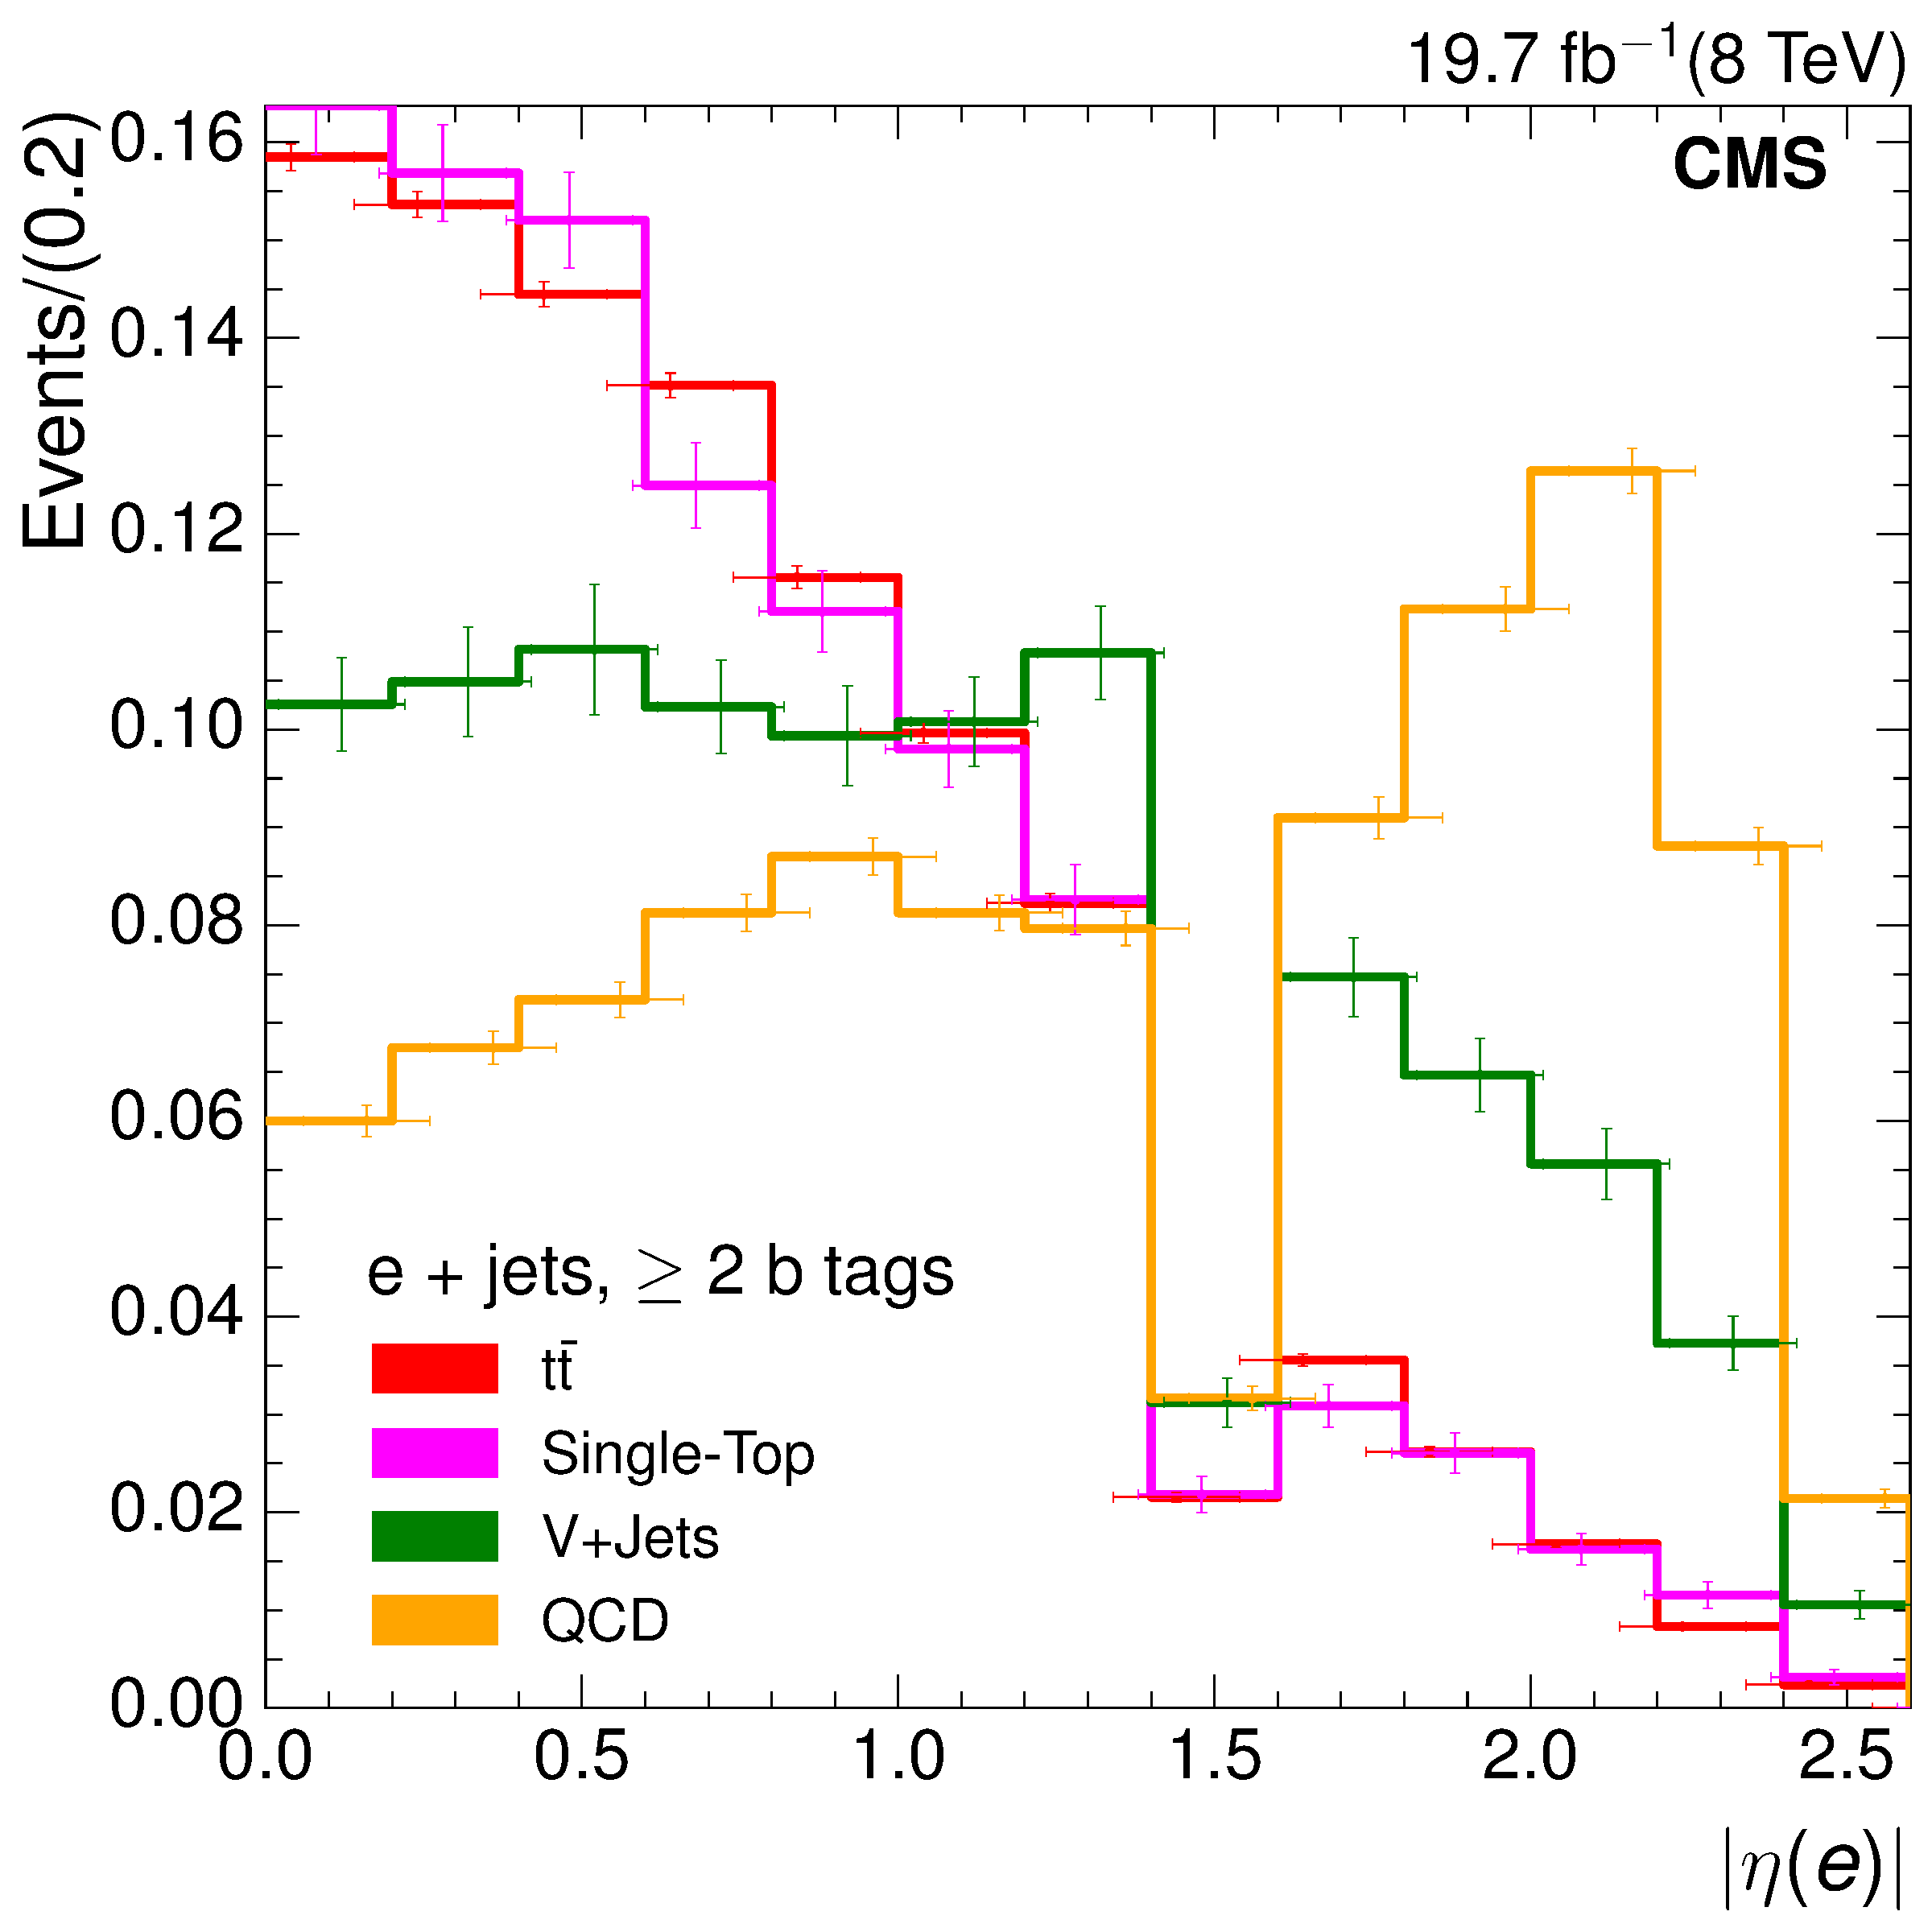
\includegraphics[width=0.45\textwidth]{Chapters/07_08_09_Analysis/Images/8TeV/fit_variables/electron/MET/electron_absolute_eta/MET_inclusive_electron_absolute_eta_2orMoreBtags_templates.pdf}\hfill
     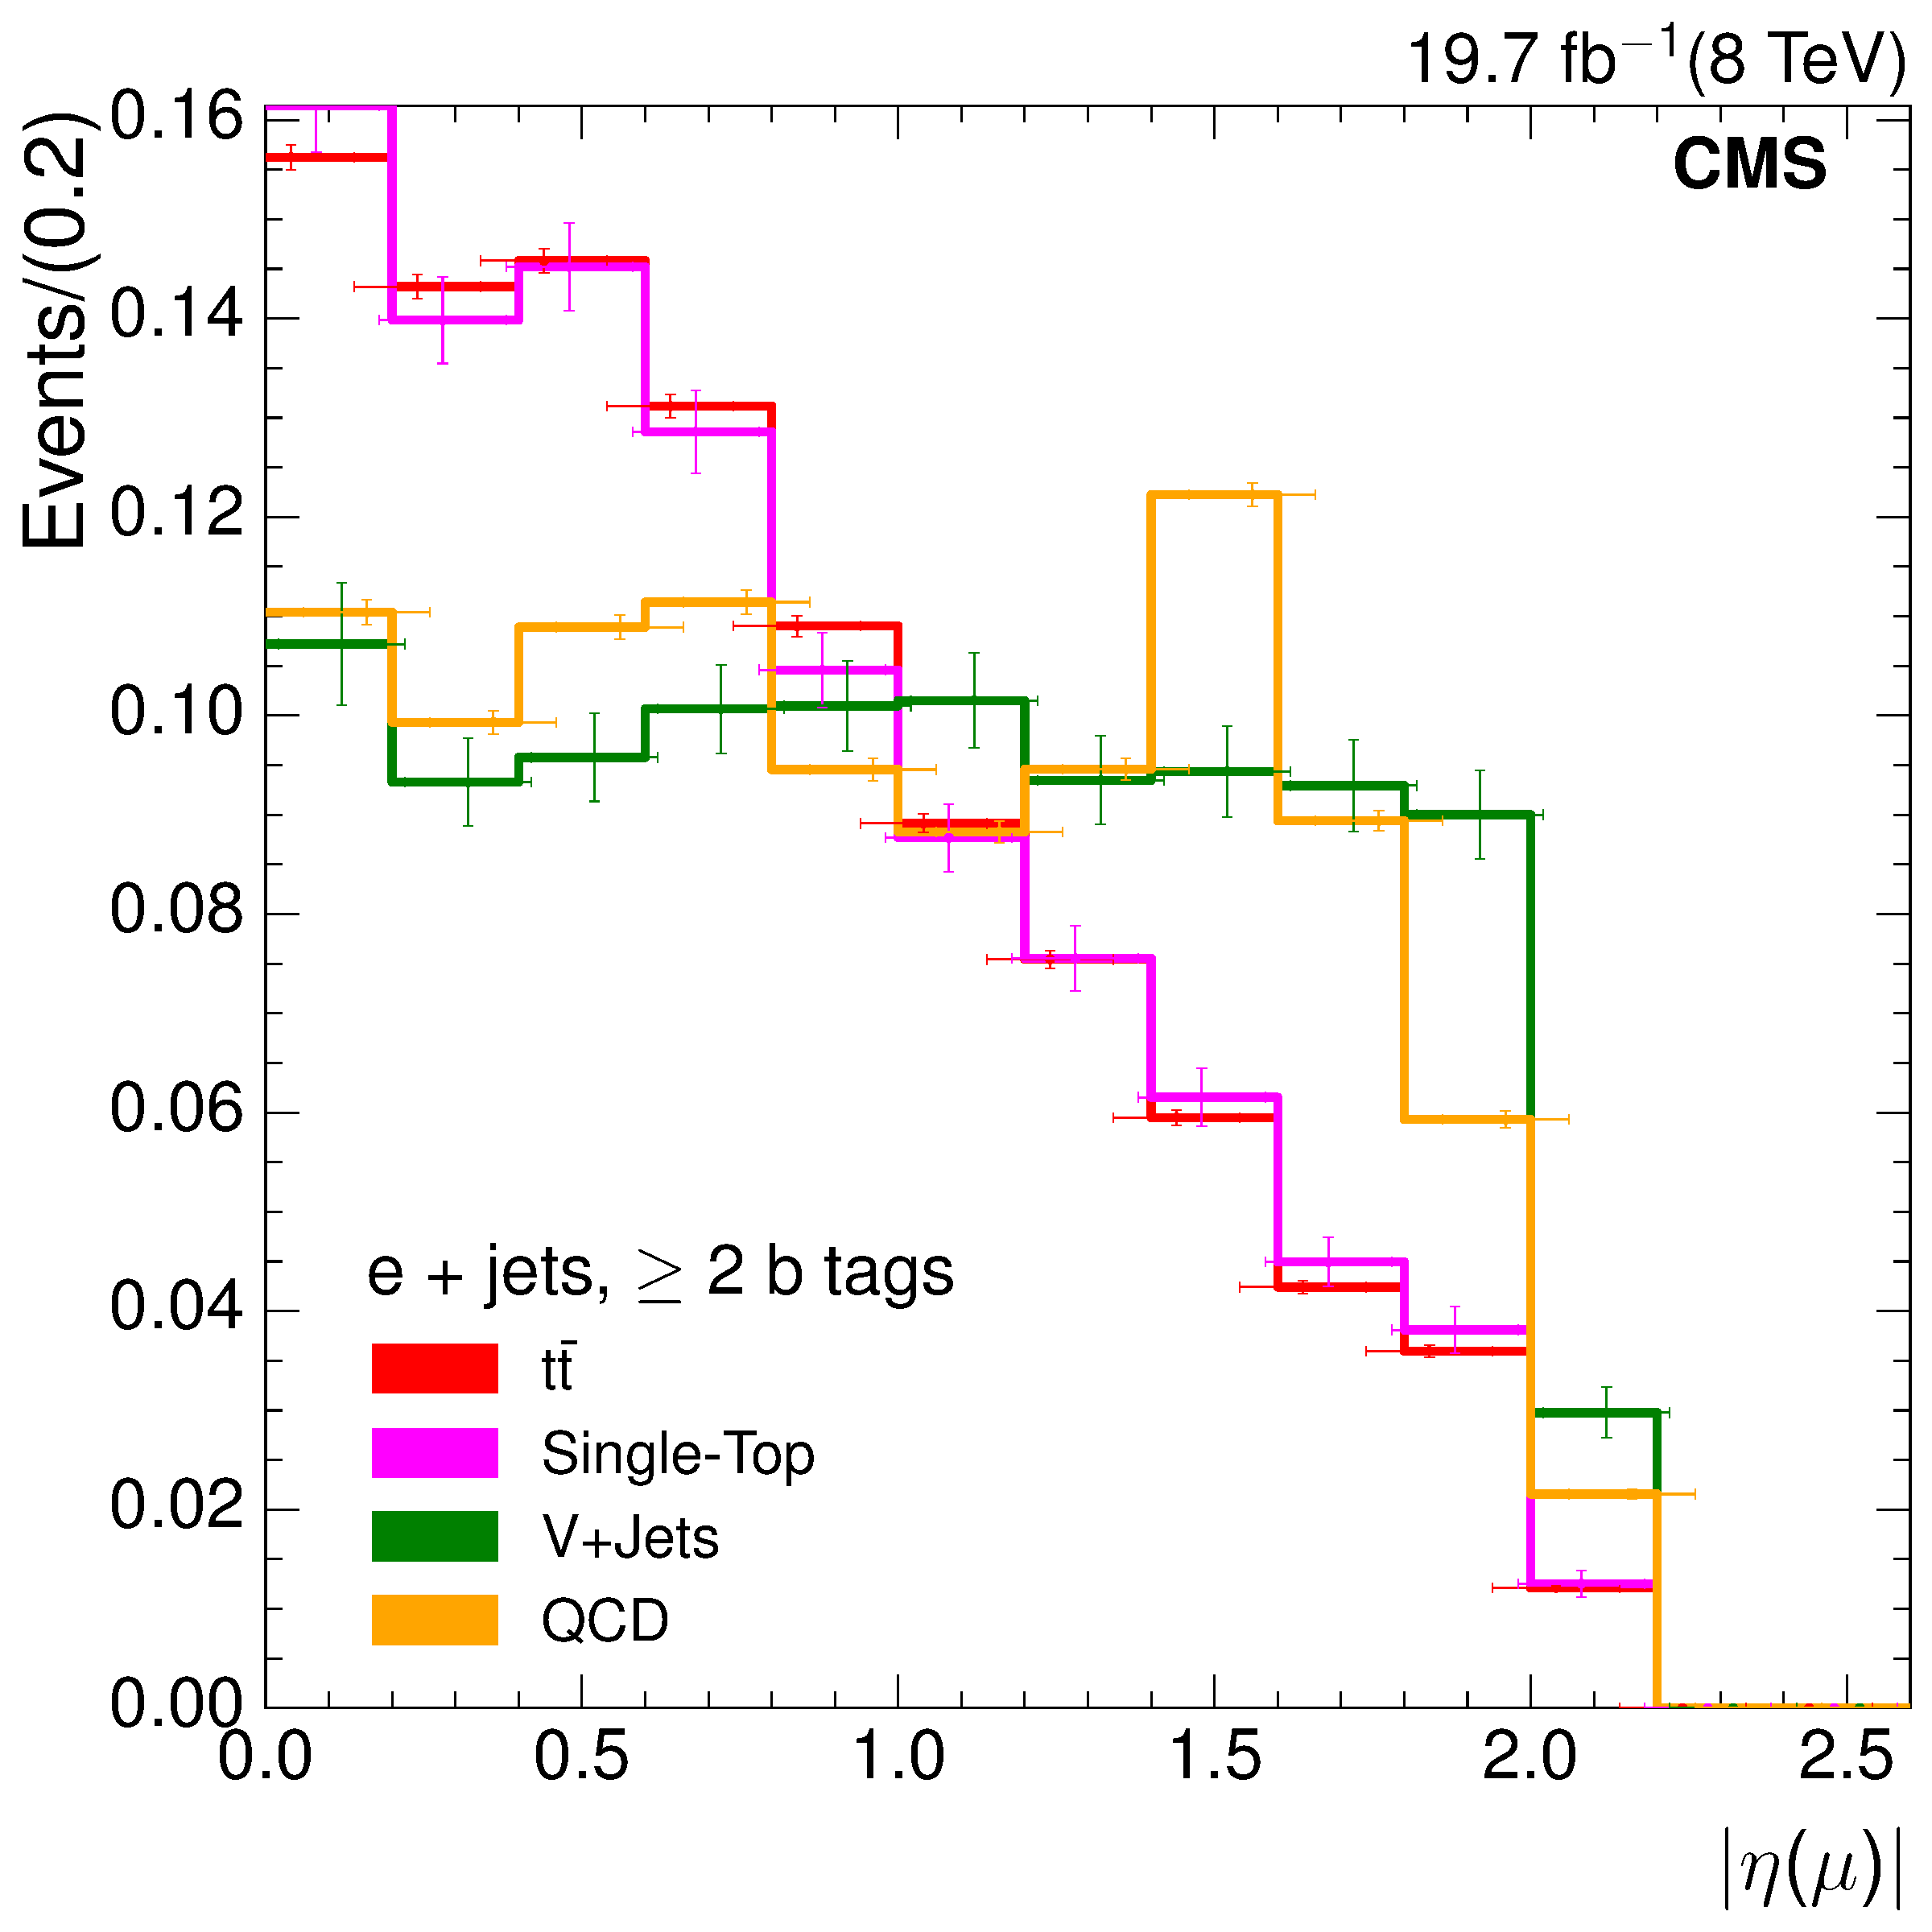
\includegraphics[width=0.45\textwidth]{Chapters/07_08_09_Analysis/Images/8TeV/fit_variables/muon/MET/muon_absolute_eta/MET_inclusive_muon_absolute_eta_2orMoreBtags_templates.pdf}\\
     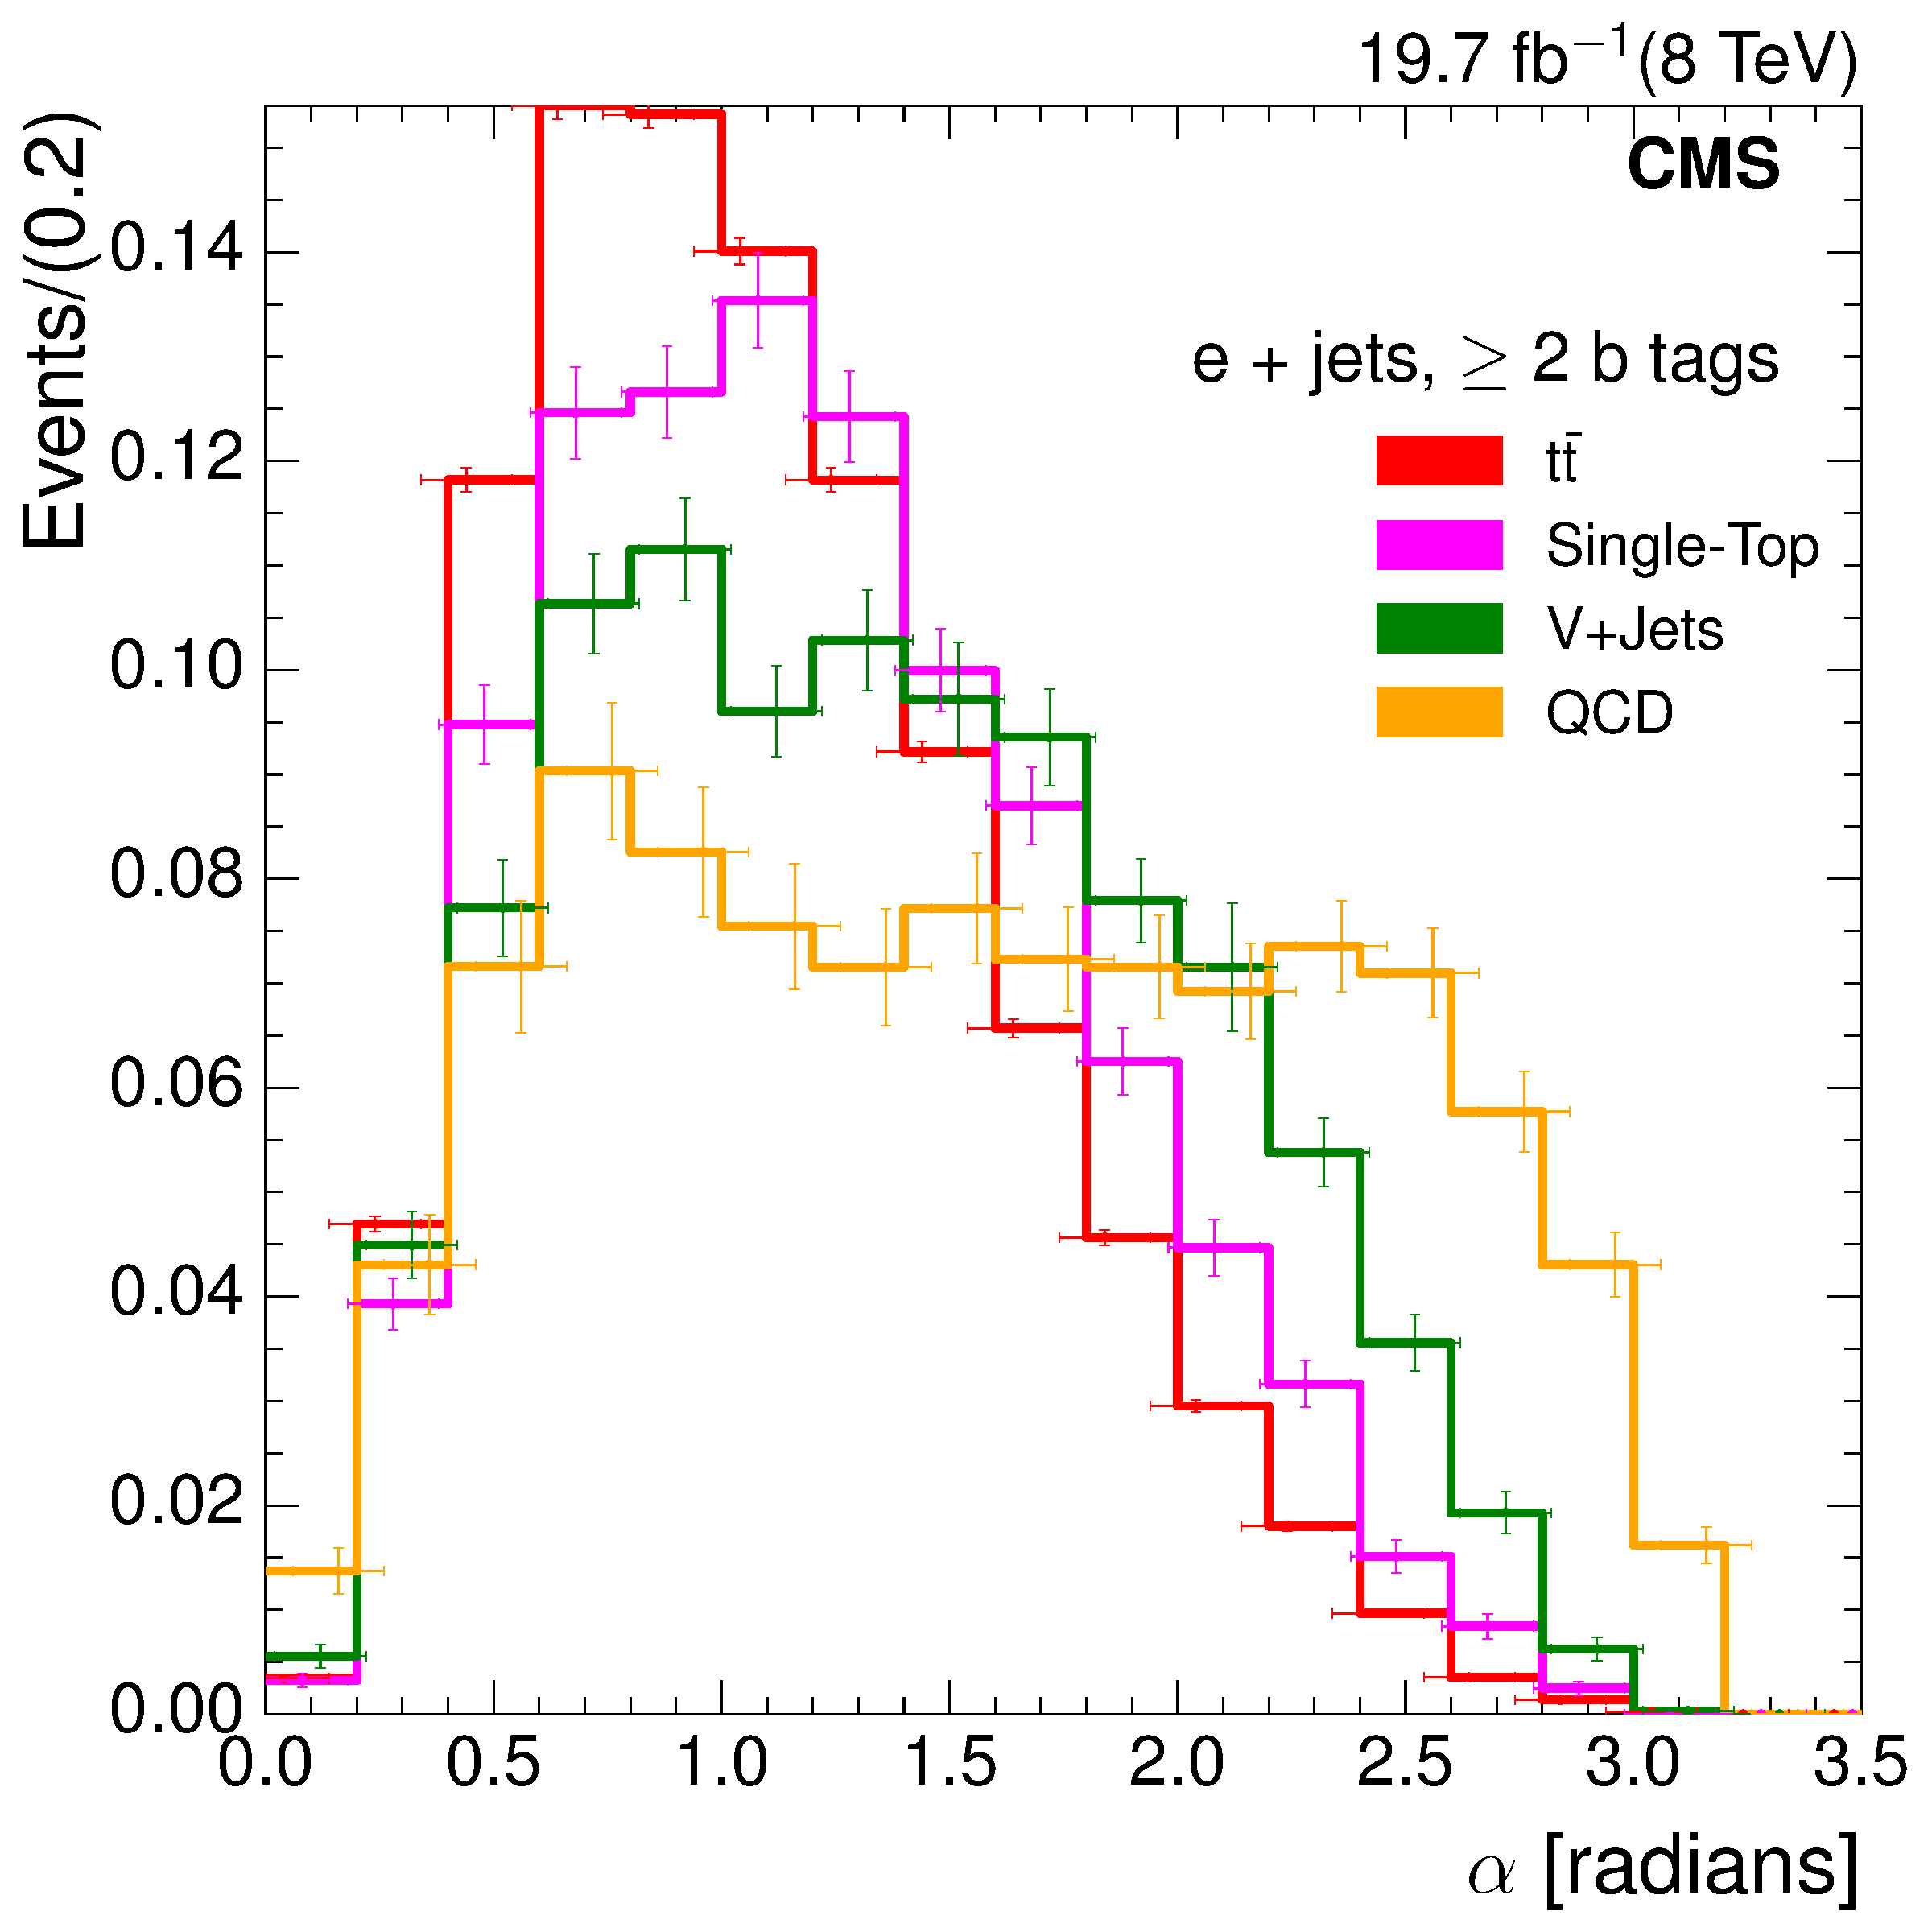
\includegraphics[width=0.45\textwidth]{Chapters/07_08_09_Analysis/Images/8TeV/fit_variables/electron/MET/angle_bl/MET_inclusive_angle_bl_2orMoreBtags_templates.pdf}\hfill
     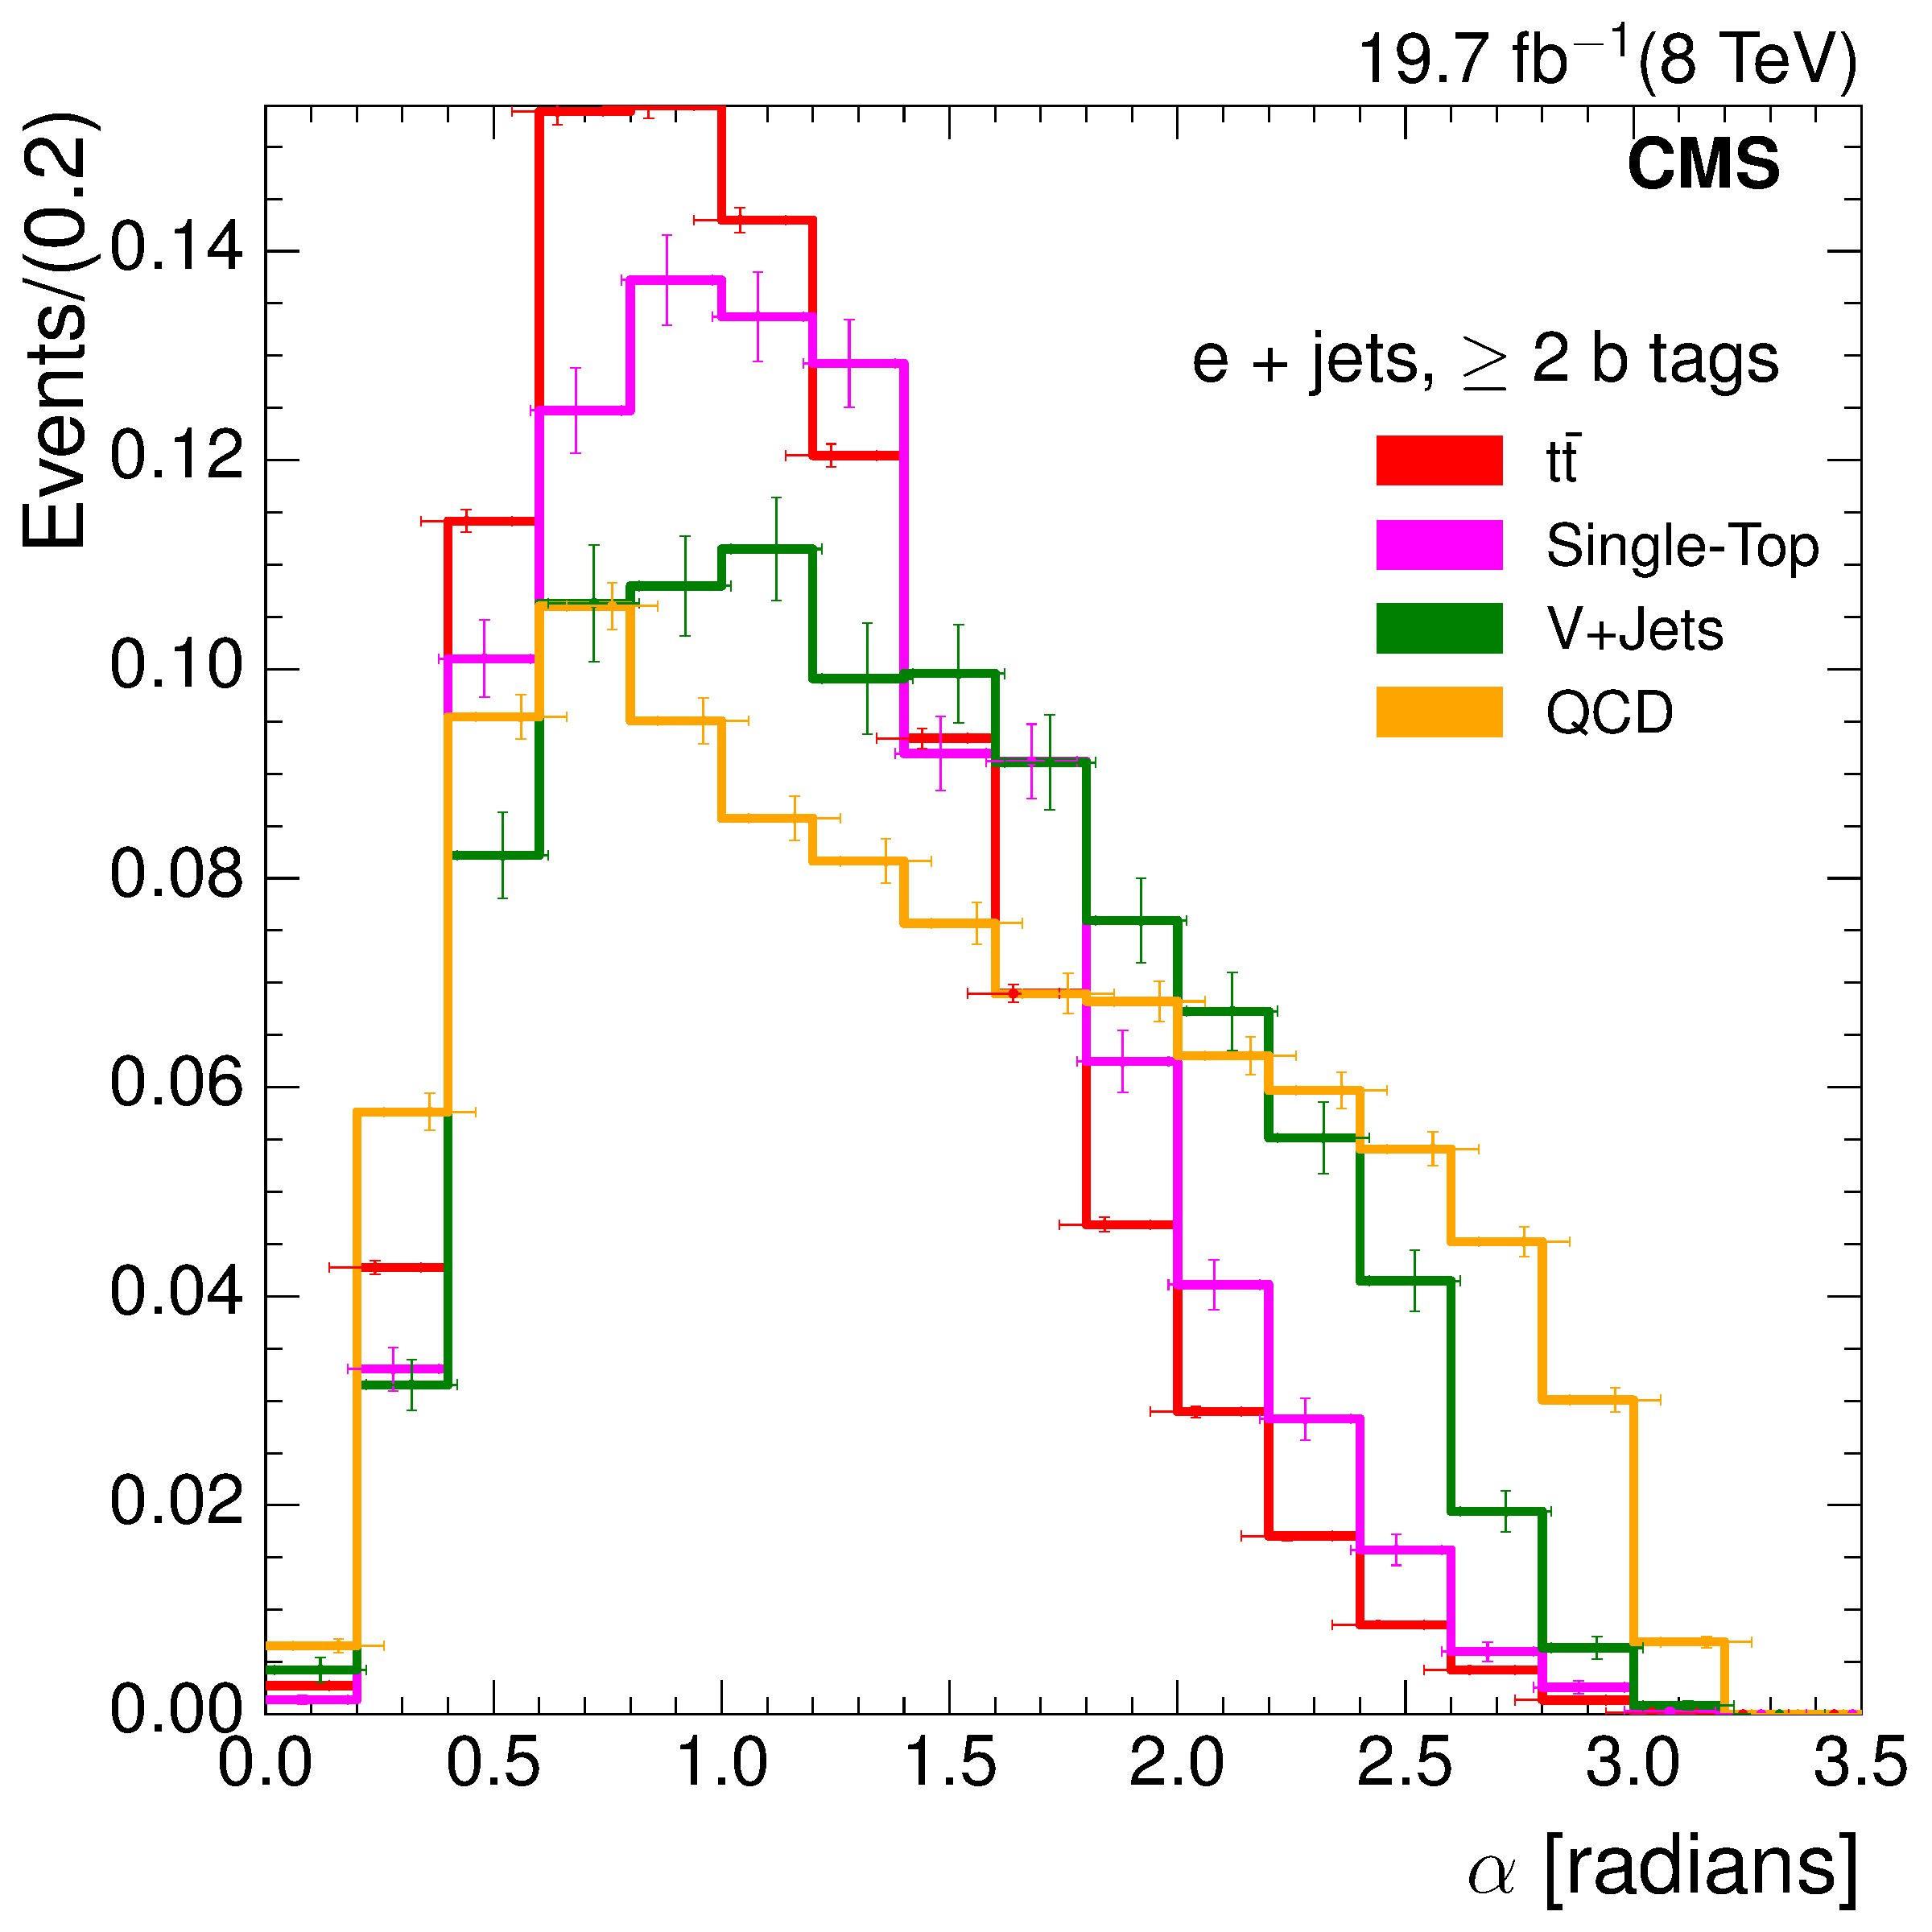
\includegraphics[width=0.45\textwidth]{Chapters/07_08_09_Analysis/Images/8TeV/fit_variables/muon/MET/angle_bl/MET_inclusive_angle_bl_2orMoreBtags_templates.pdf}\\
     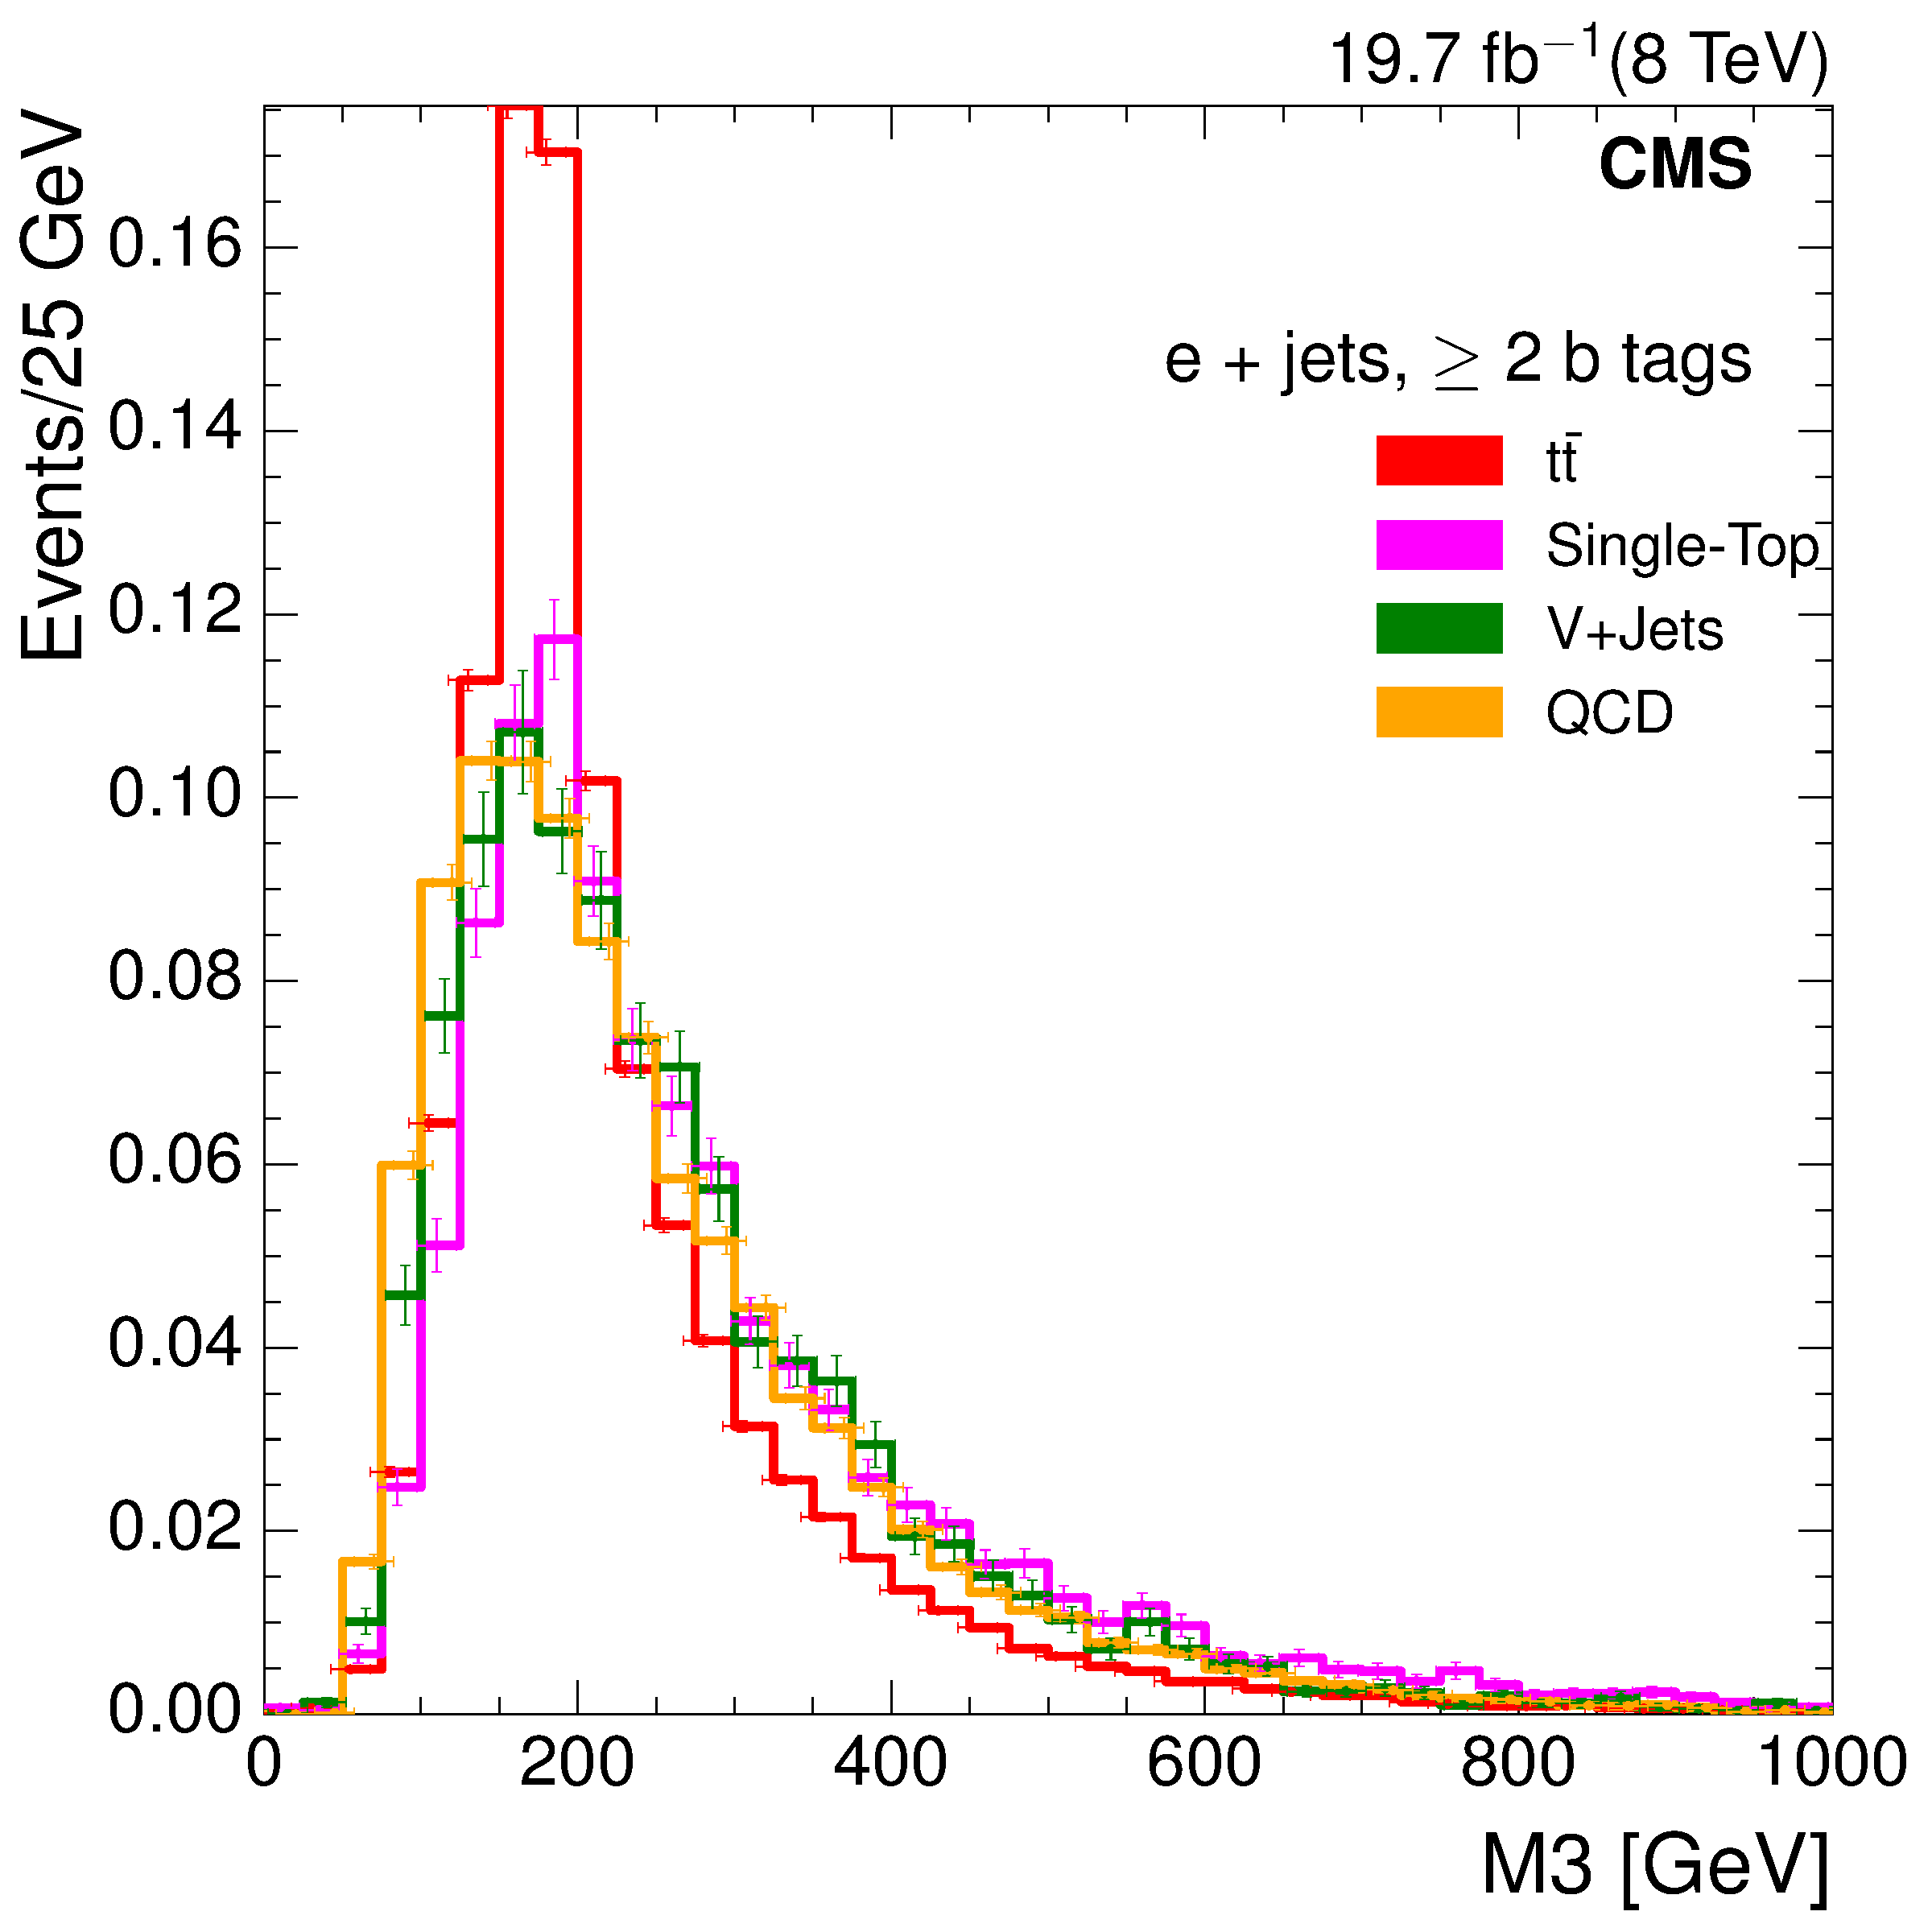
\includegraphics[width=0.45\textwidth]{Chapters/07_08_09_Analysis/Images/8TeV/fit_variables/electron/MET/M3/MET_inclusive_M3_2orMoreBtags_templates.pdf}\hfill
     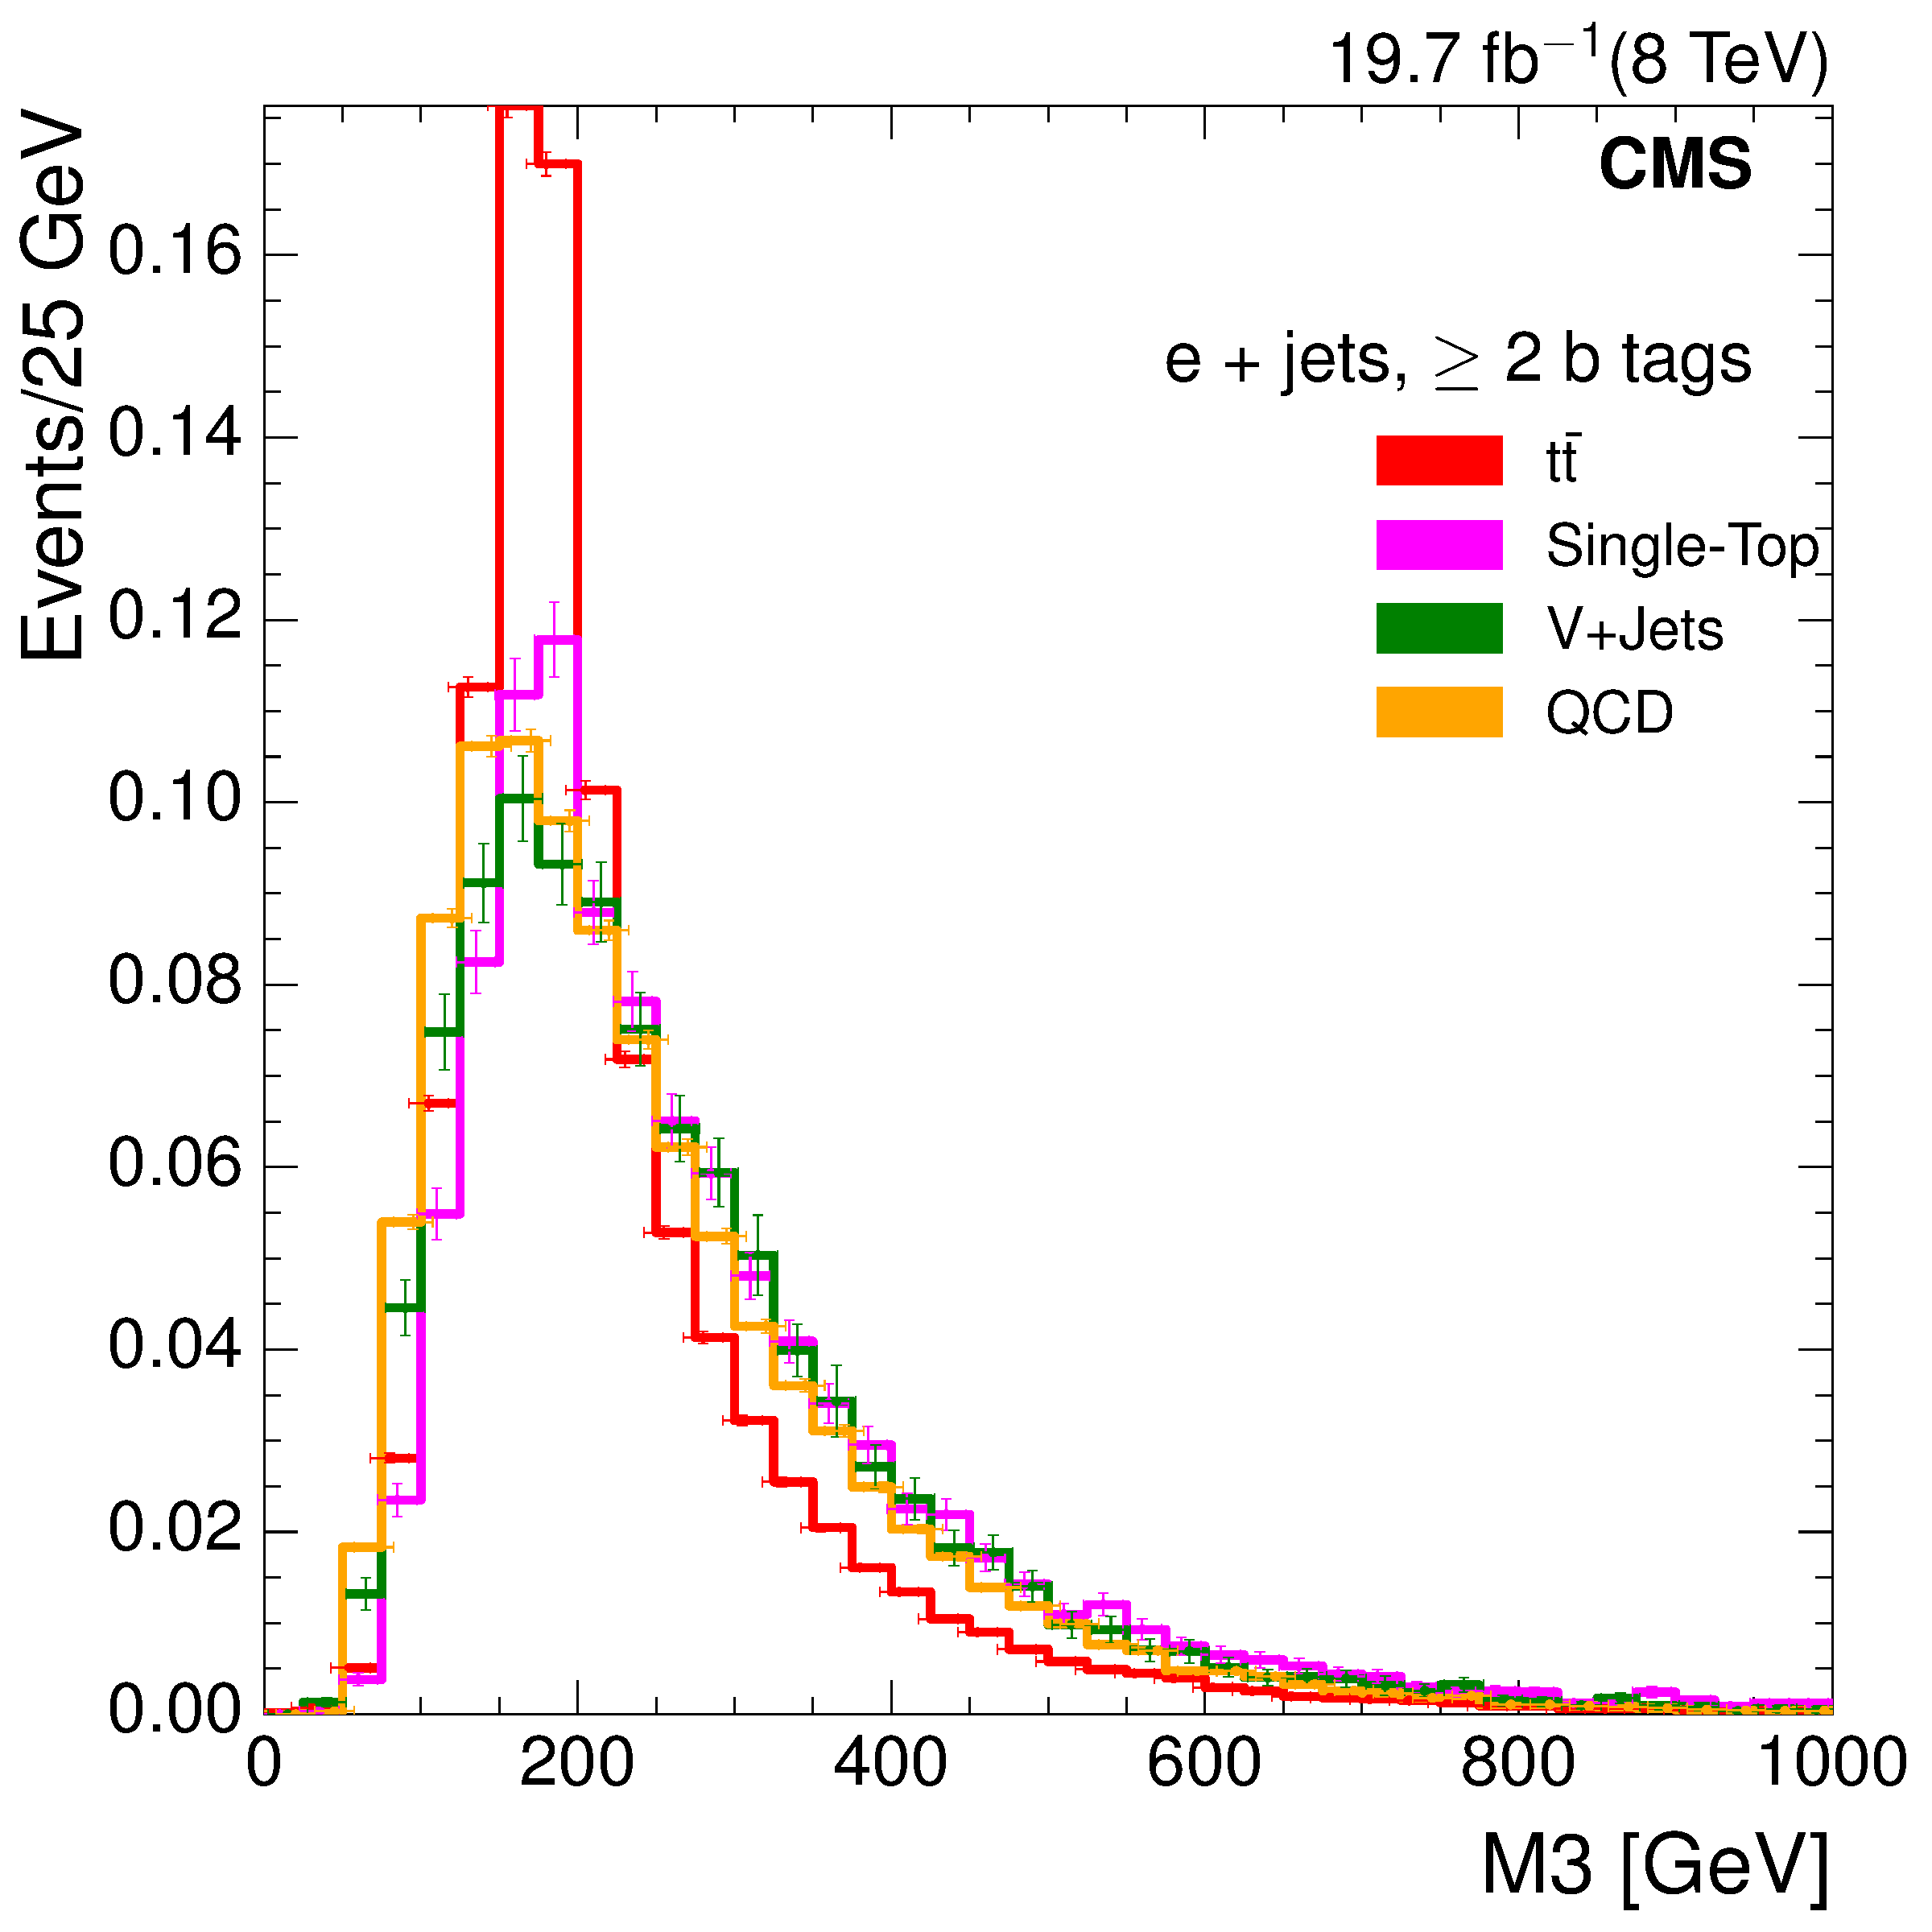
\includegraphics[width=0.45\textwidth]{Chapters/07_08_09_Analysis/Images/8TeV/fit_variables/muon/MET/M3/MET_inclusive_M3_2orMoreBtags_templates.pdf}\\
	 \caption[Normalised distributions of the templates for the three fit variables inclusive
	 across all primary variable bins at $\sqrt{s}=8\TeV$.]{Normalised distributions of
	 the templates for the three fit variables lepton \abseta (upper), $\alpha$ (middle) and M3 (lower) inclusive
	 across all primary variable bins at $\sqrt{s}=8\TeV$ in the electron+jets channel (left) and in the
	 muon+jets channel (right).}
     \label{fig:fit_variable_distributions_8TeV}
\end{figure}

% Removed from appendices:
% \section{Fitting variable QCD background template comparisons}
% \label{as:fitting_variable_QCD_template_comparisons}
% 
% \begin{figure}[hbtp]
%     \centering
%      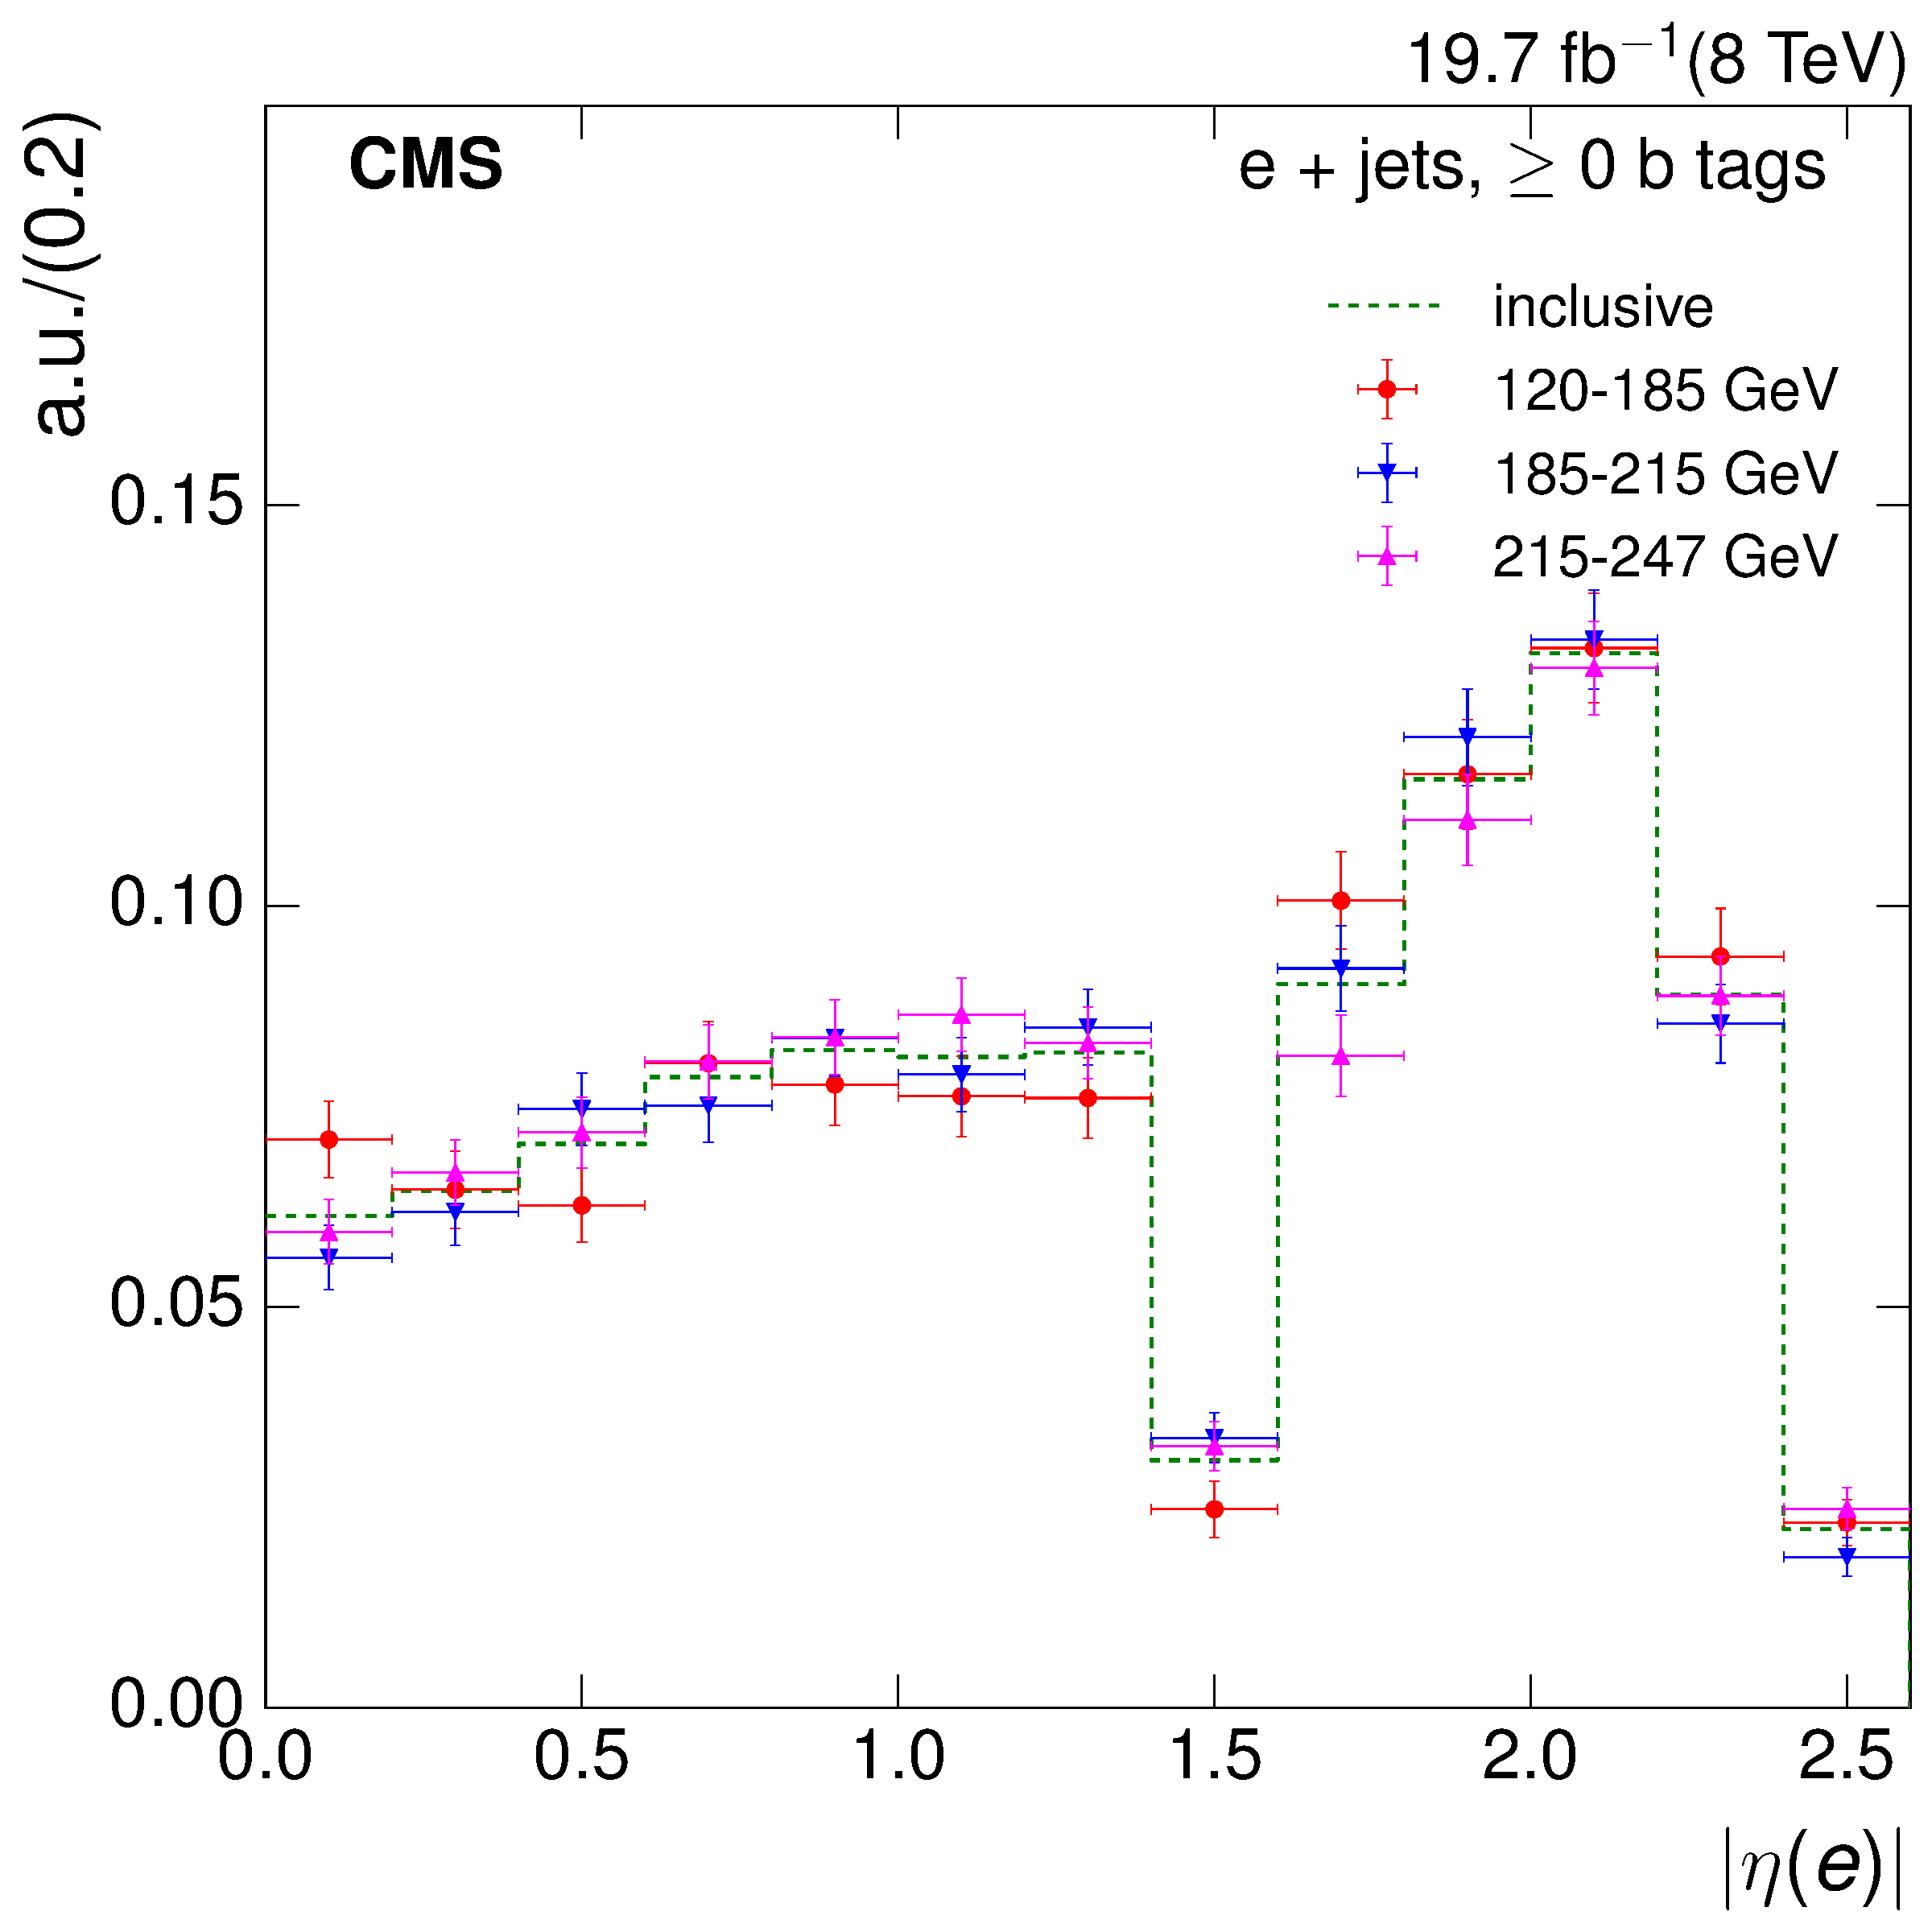
\includegraphics[width=0.48\textwidth]{Chapters/07_08_09_Analysis/Images/8TeV/fit_variables/electron/HT/electron_absolute_eta/qcd/HT_electron_absolute_eta_0orMoreBtag_QCD_template_comparison.pdf}\hfill
%      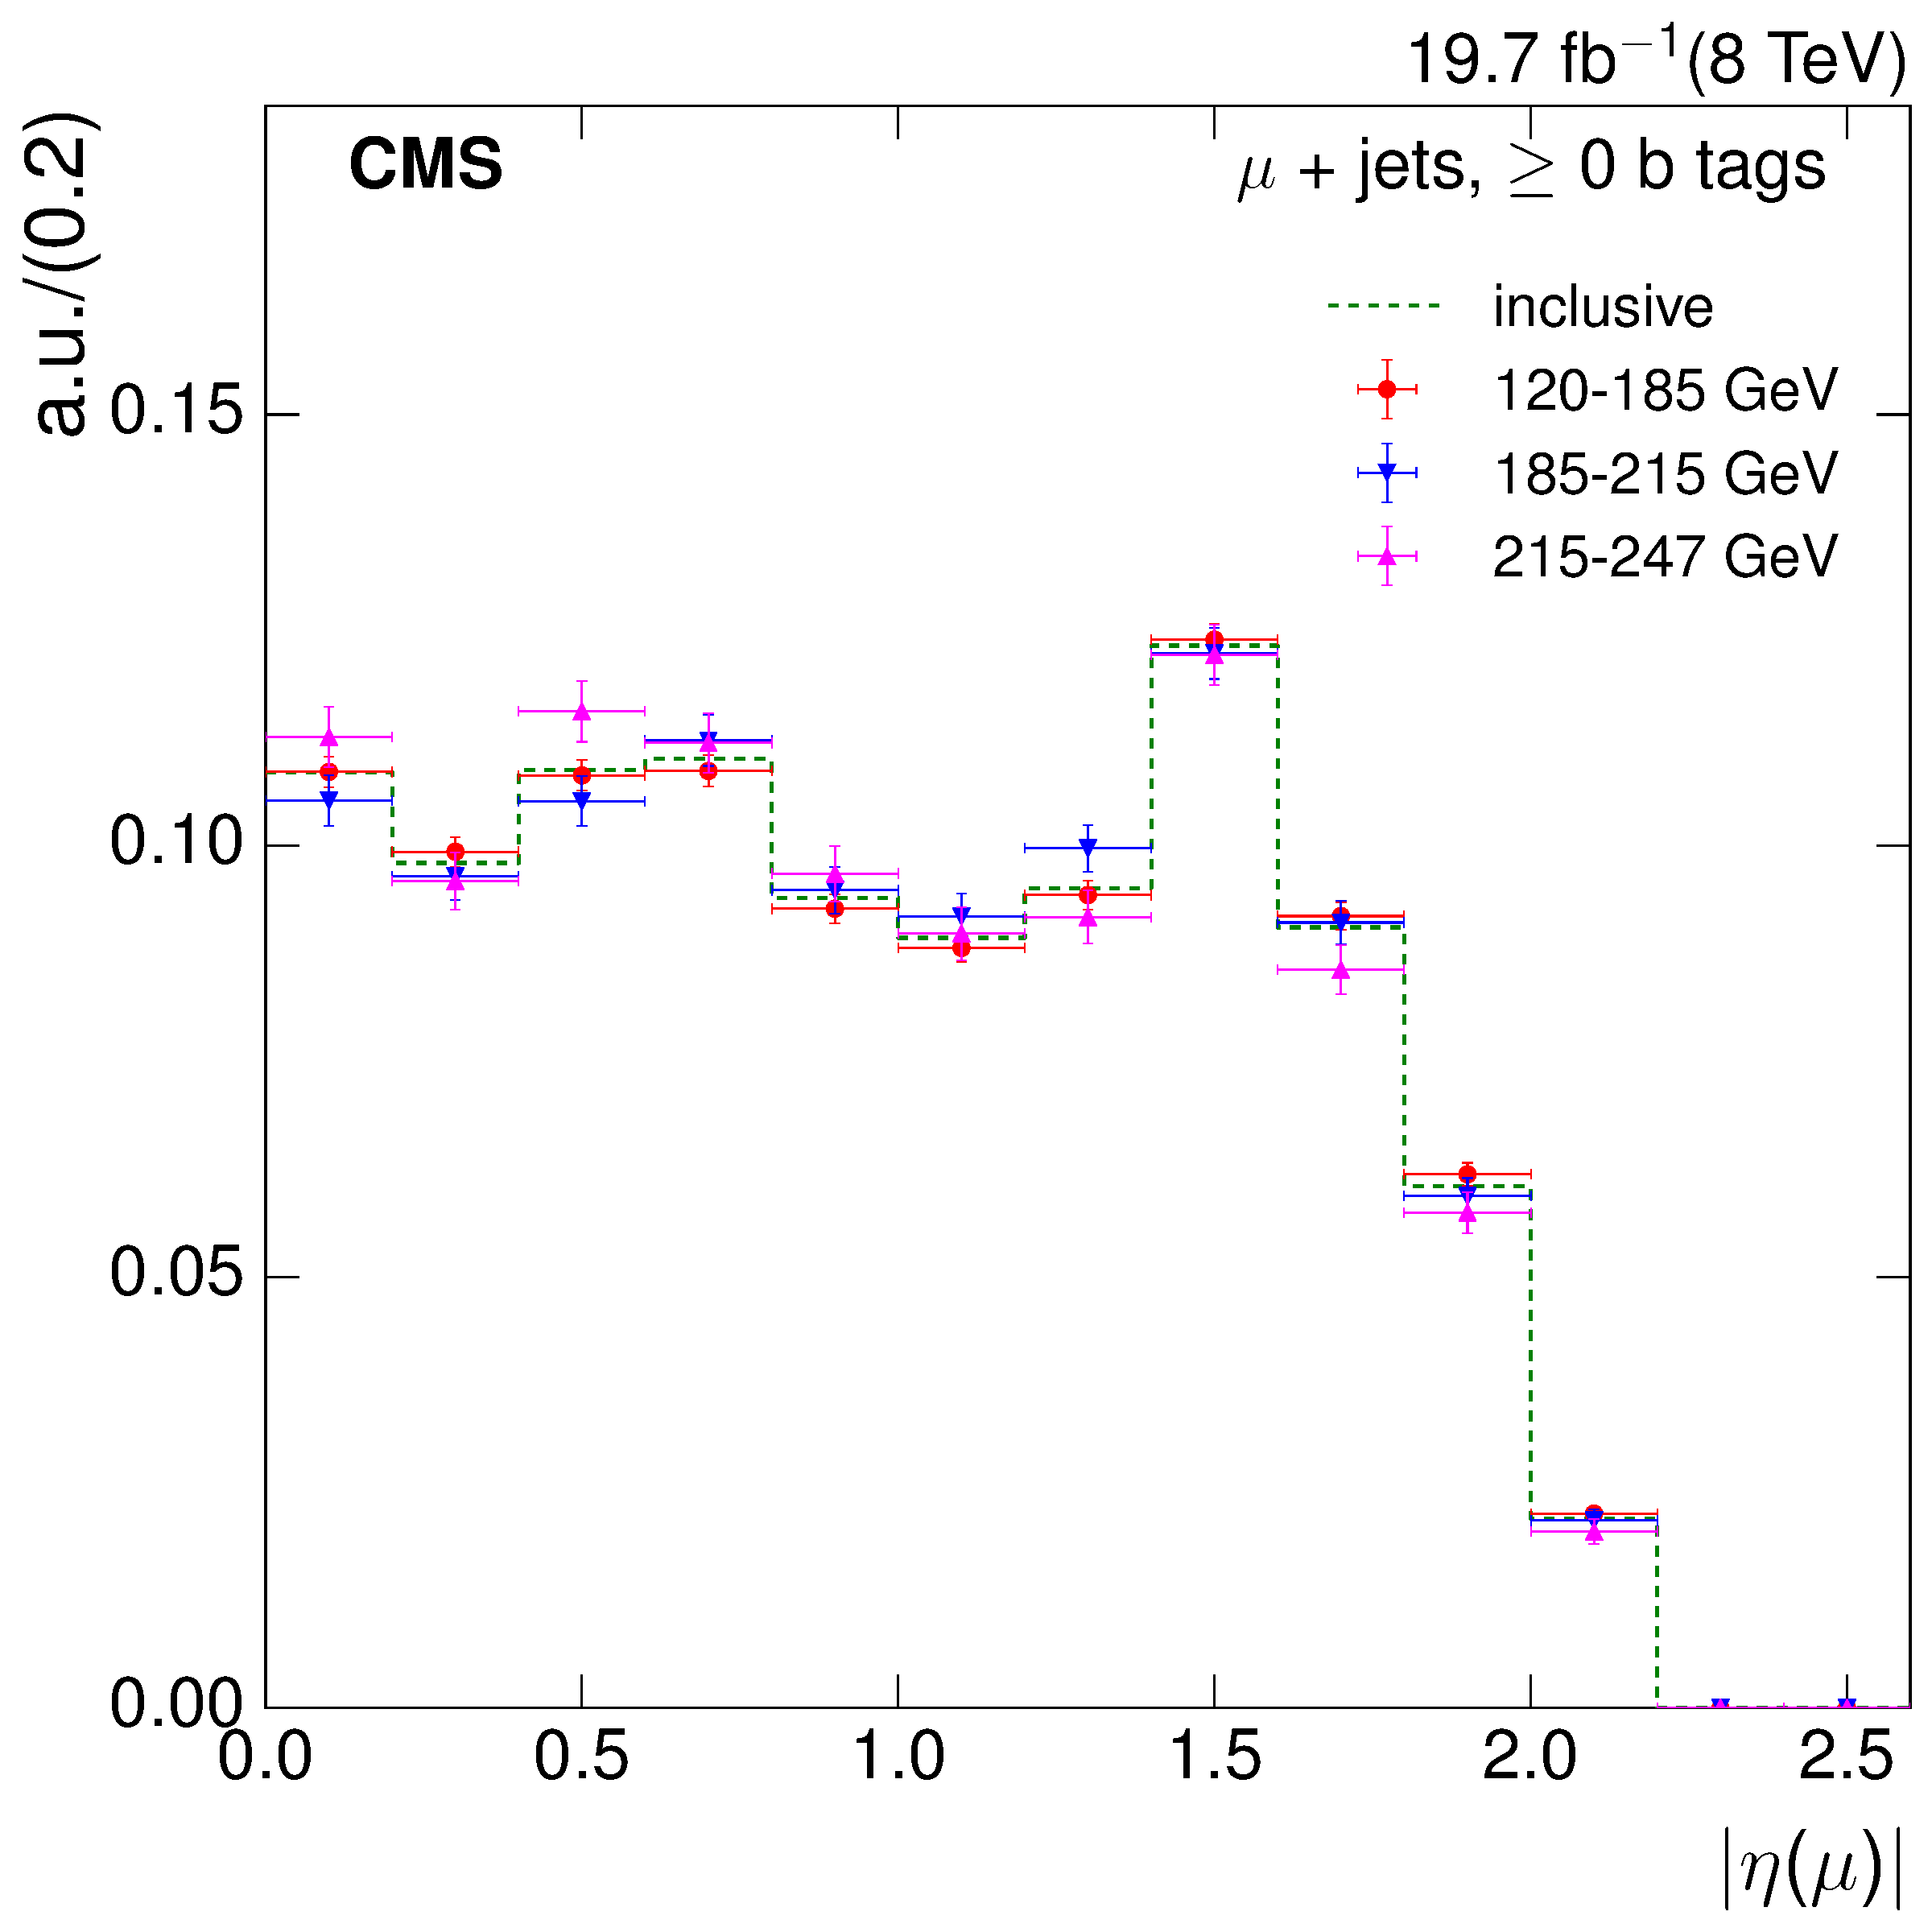
\includegraphics[width=0.48\textwidth]{Chapters/07_08_09_Analysis/Images/8TeV/fit_variables/muon/HT/muon_absolute_eta/qcd/HT_muon_absolute_eta_0orMoreBtag_QCD_template_comparison.pdf}\\
%      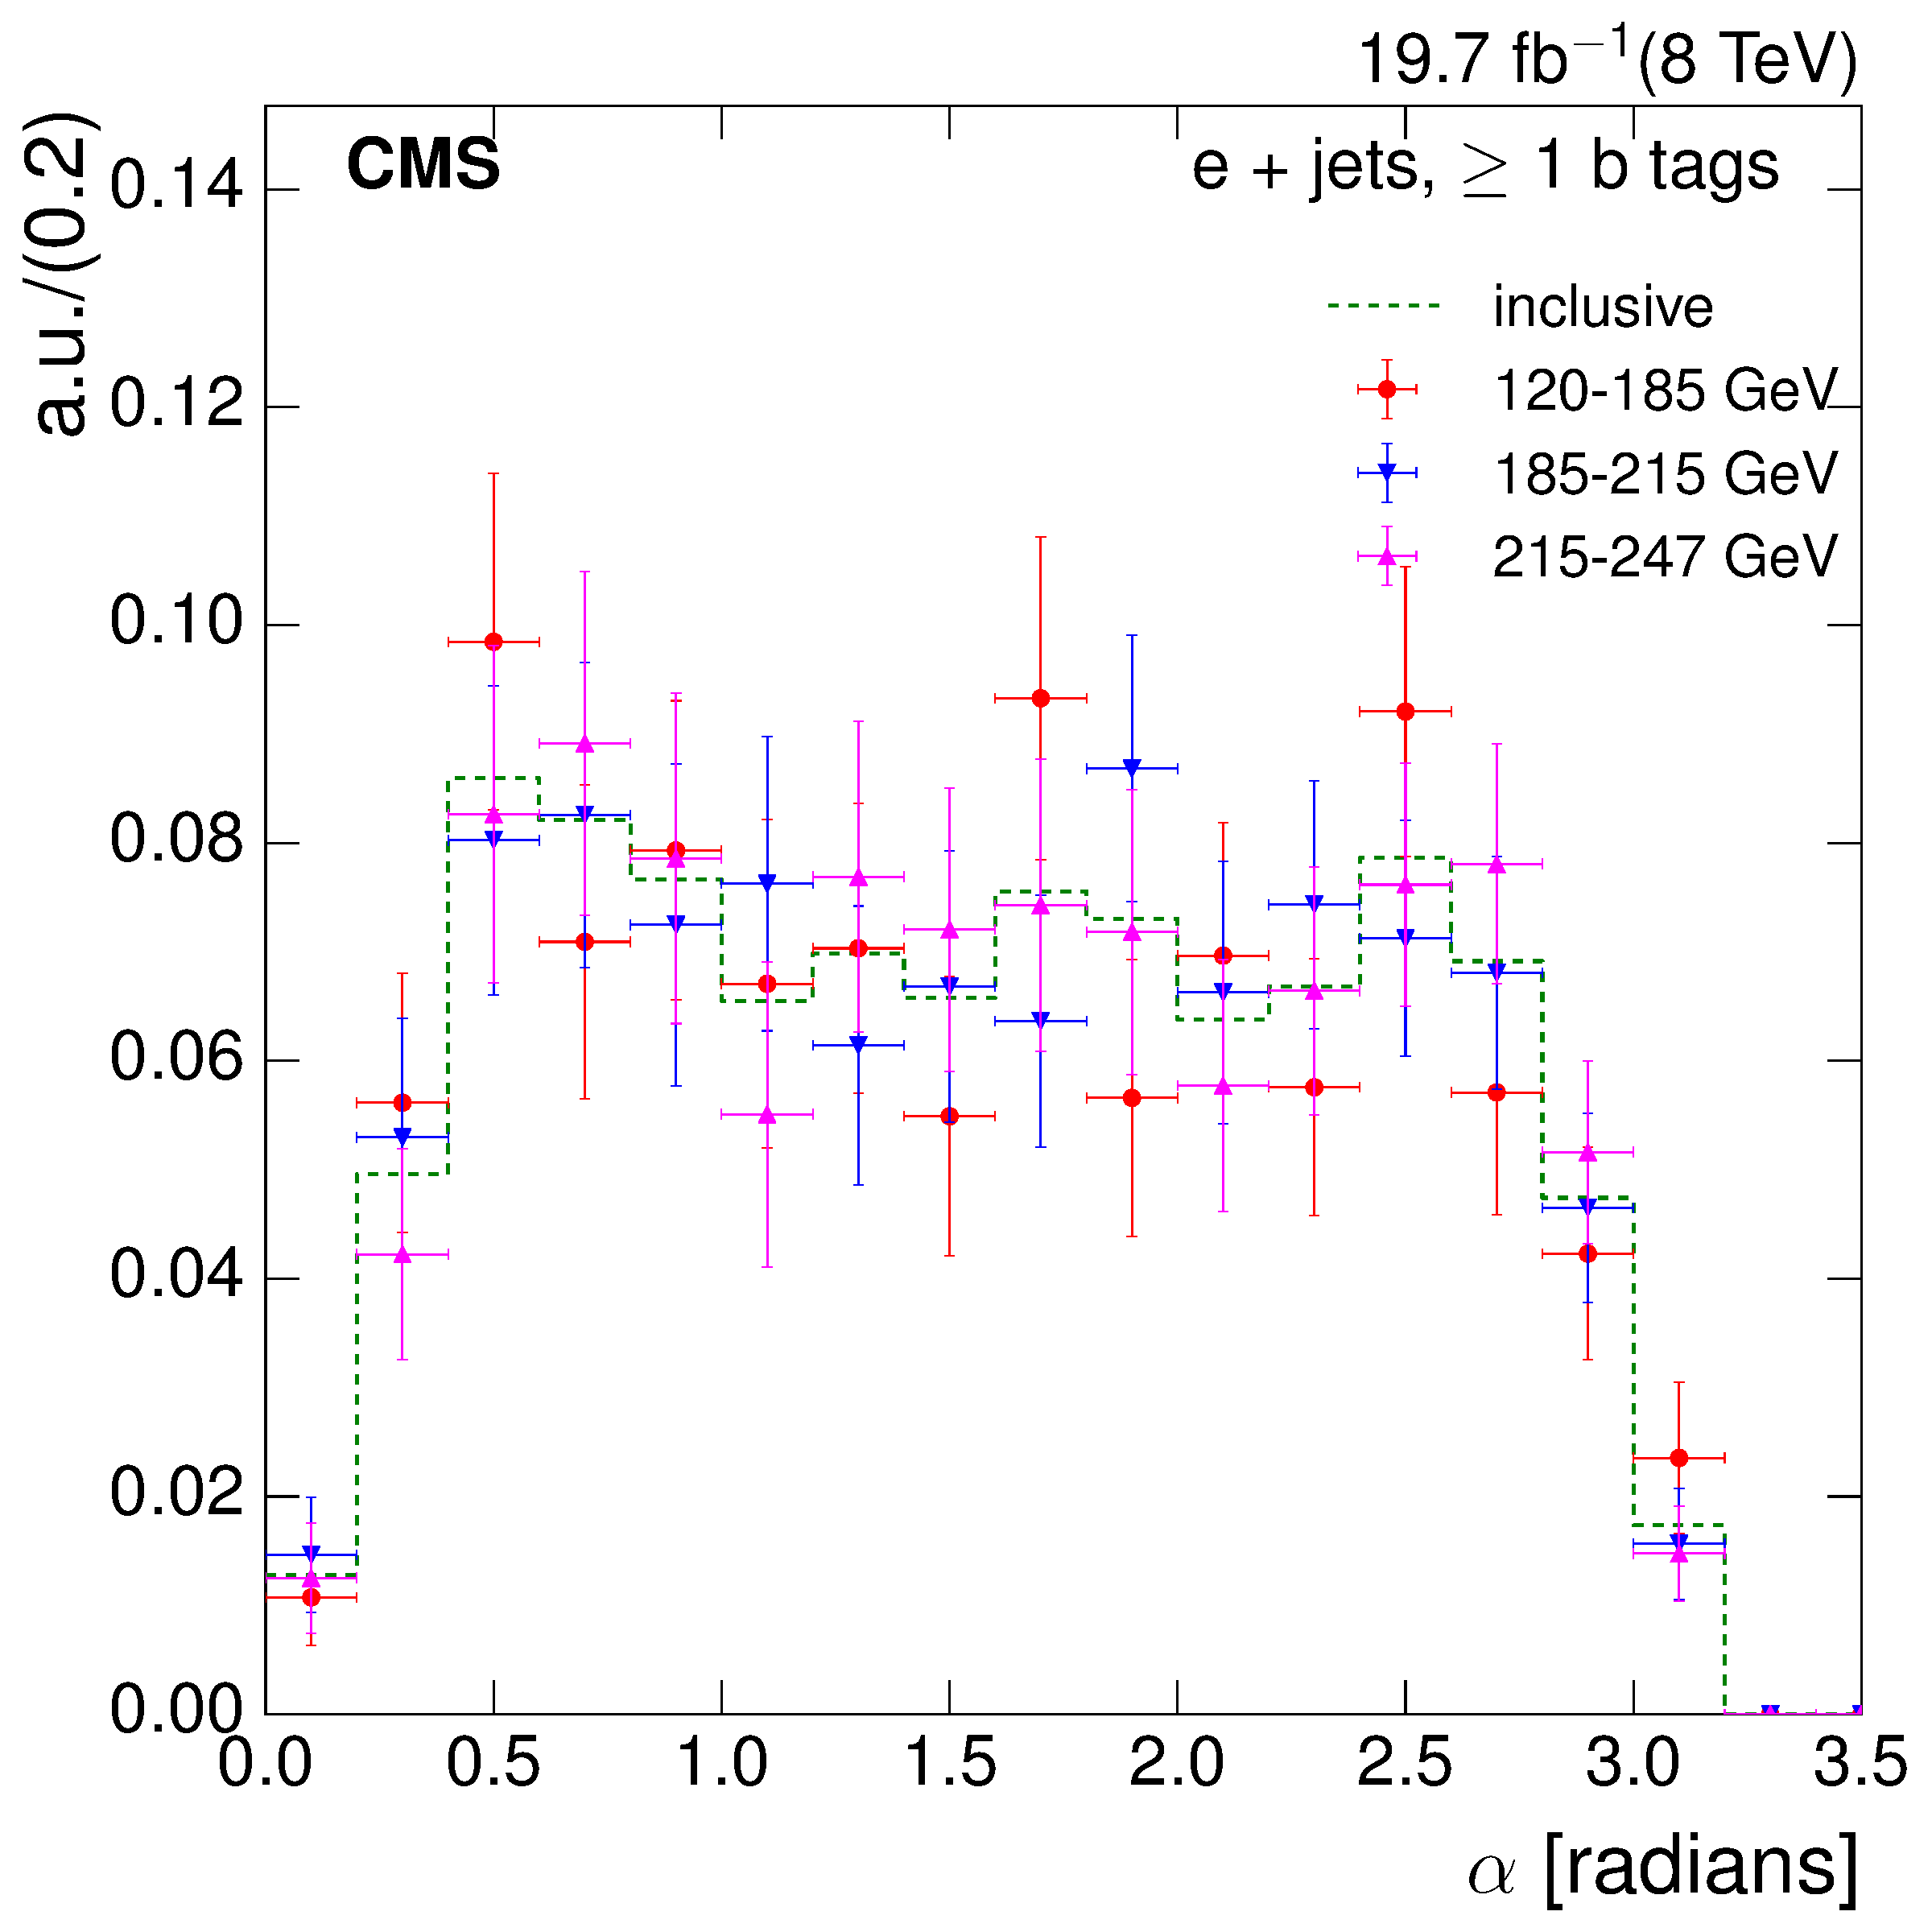
\includegraphics[width=0.48\textwidth]{Chapters/07_08_09_Analysis/Images/8TeV/fit_variables/electron/HT/angle_bl/qcd/HT_angle_bl_1orMoreBtag_QCD_template_comparison.pdf}\hfill
%      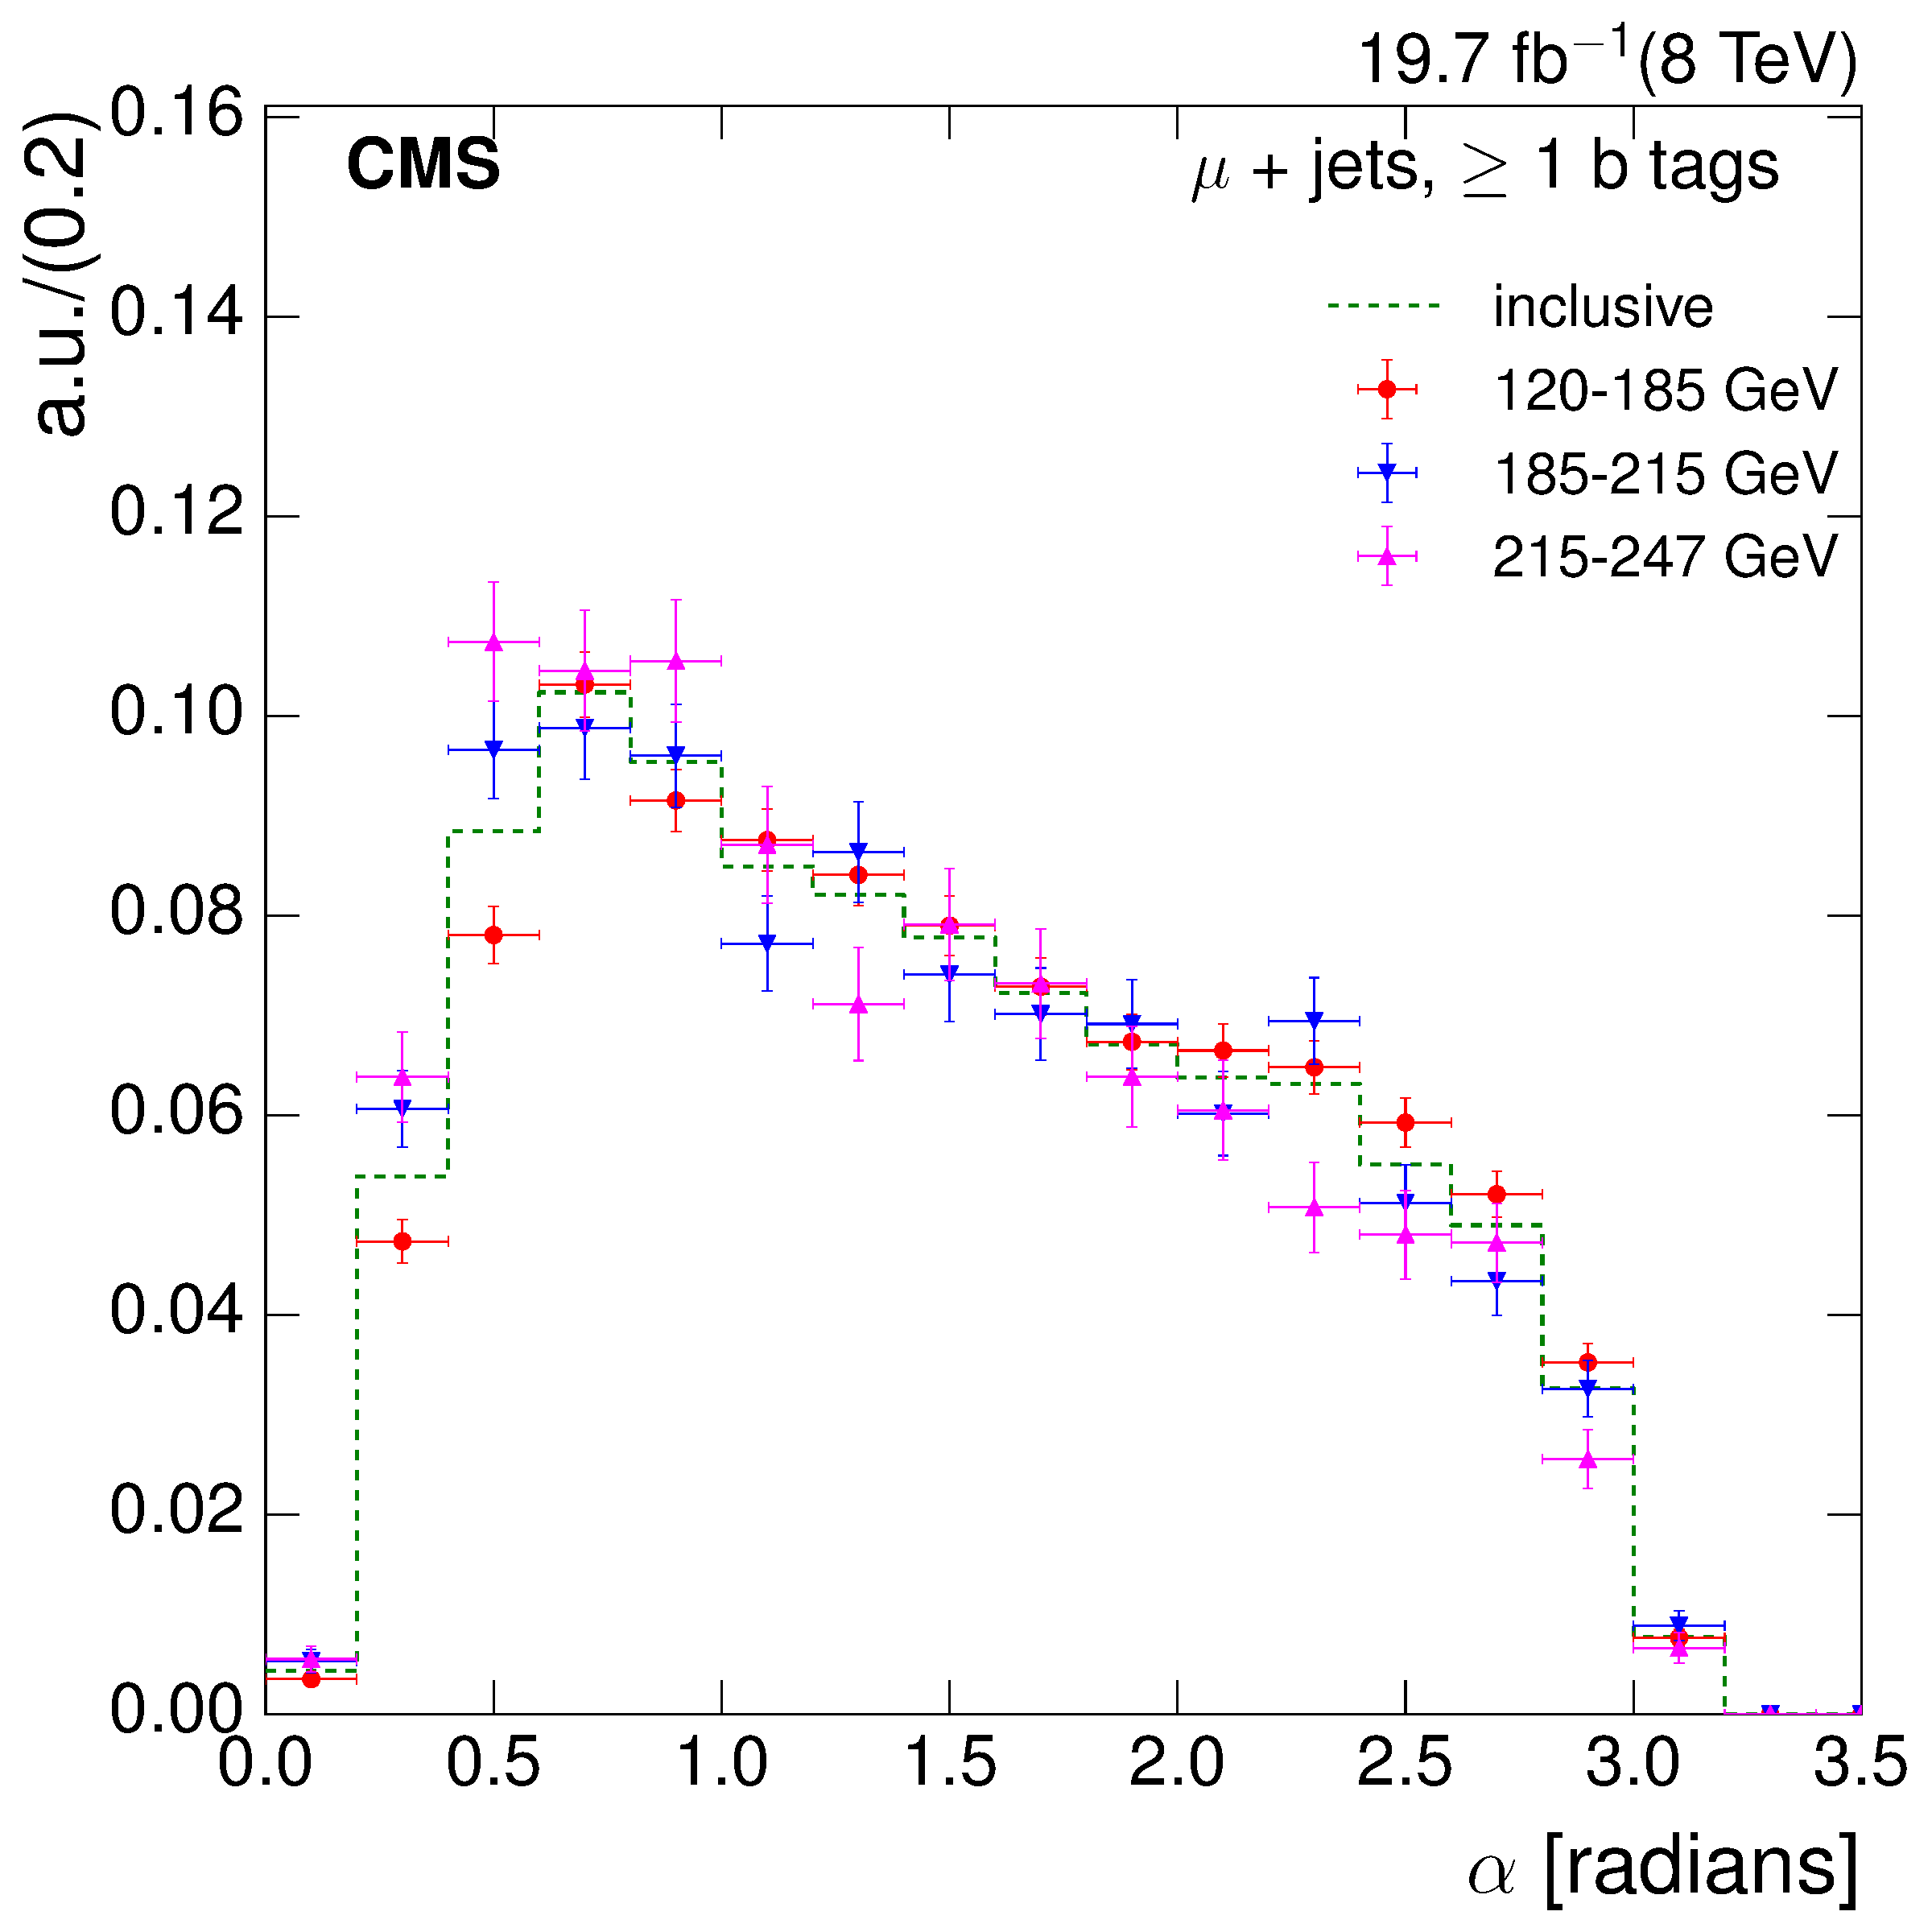
\includegraphics[width=0.48\textwidth]{Chapters/07_08_09_Analysis/Images/8TeV/fit_variables/muon/HT/angle_bl/qcd/HT_angle_bl_1orMoreBtag_QCD_template_comparison.pdf}\\
%      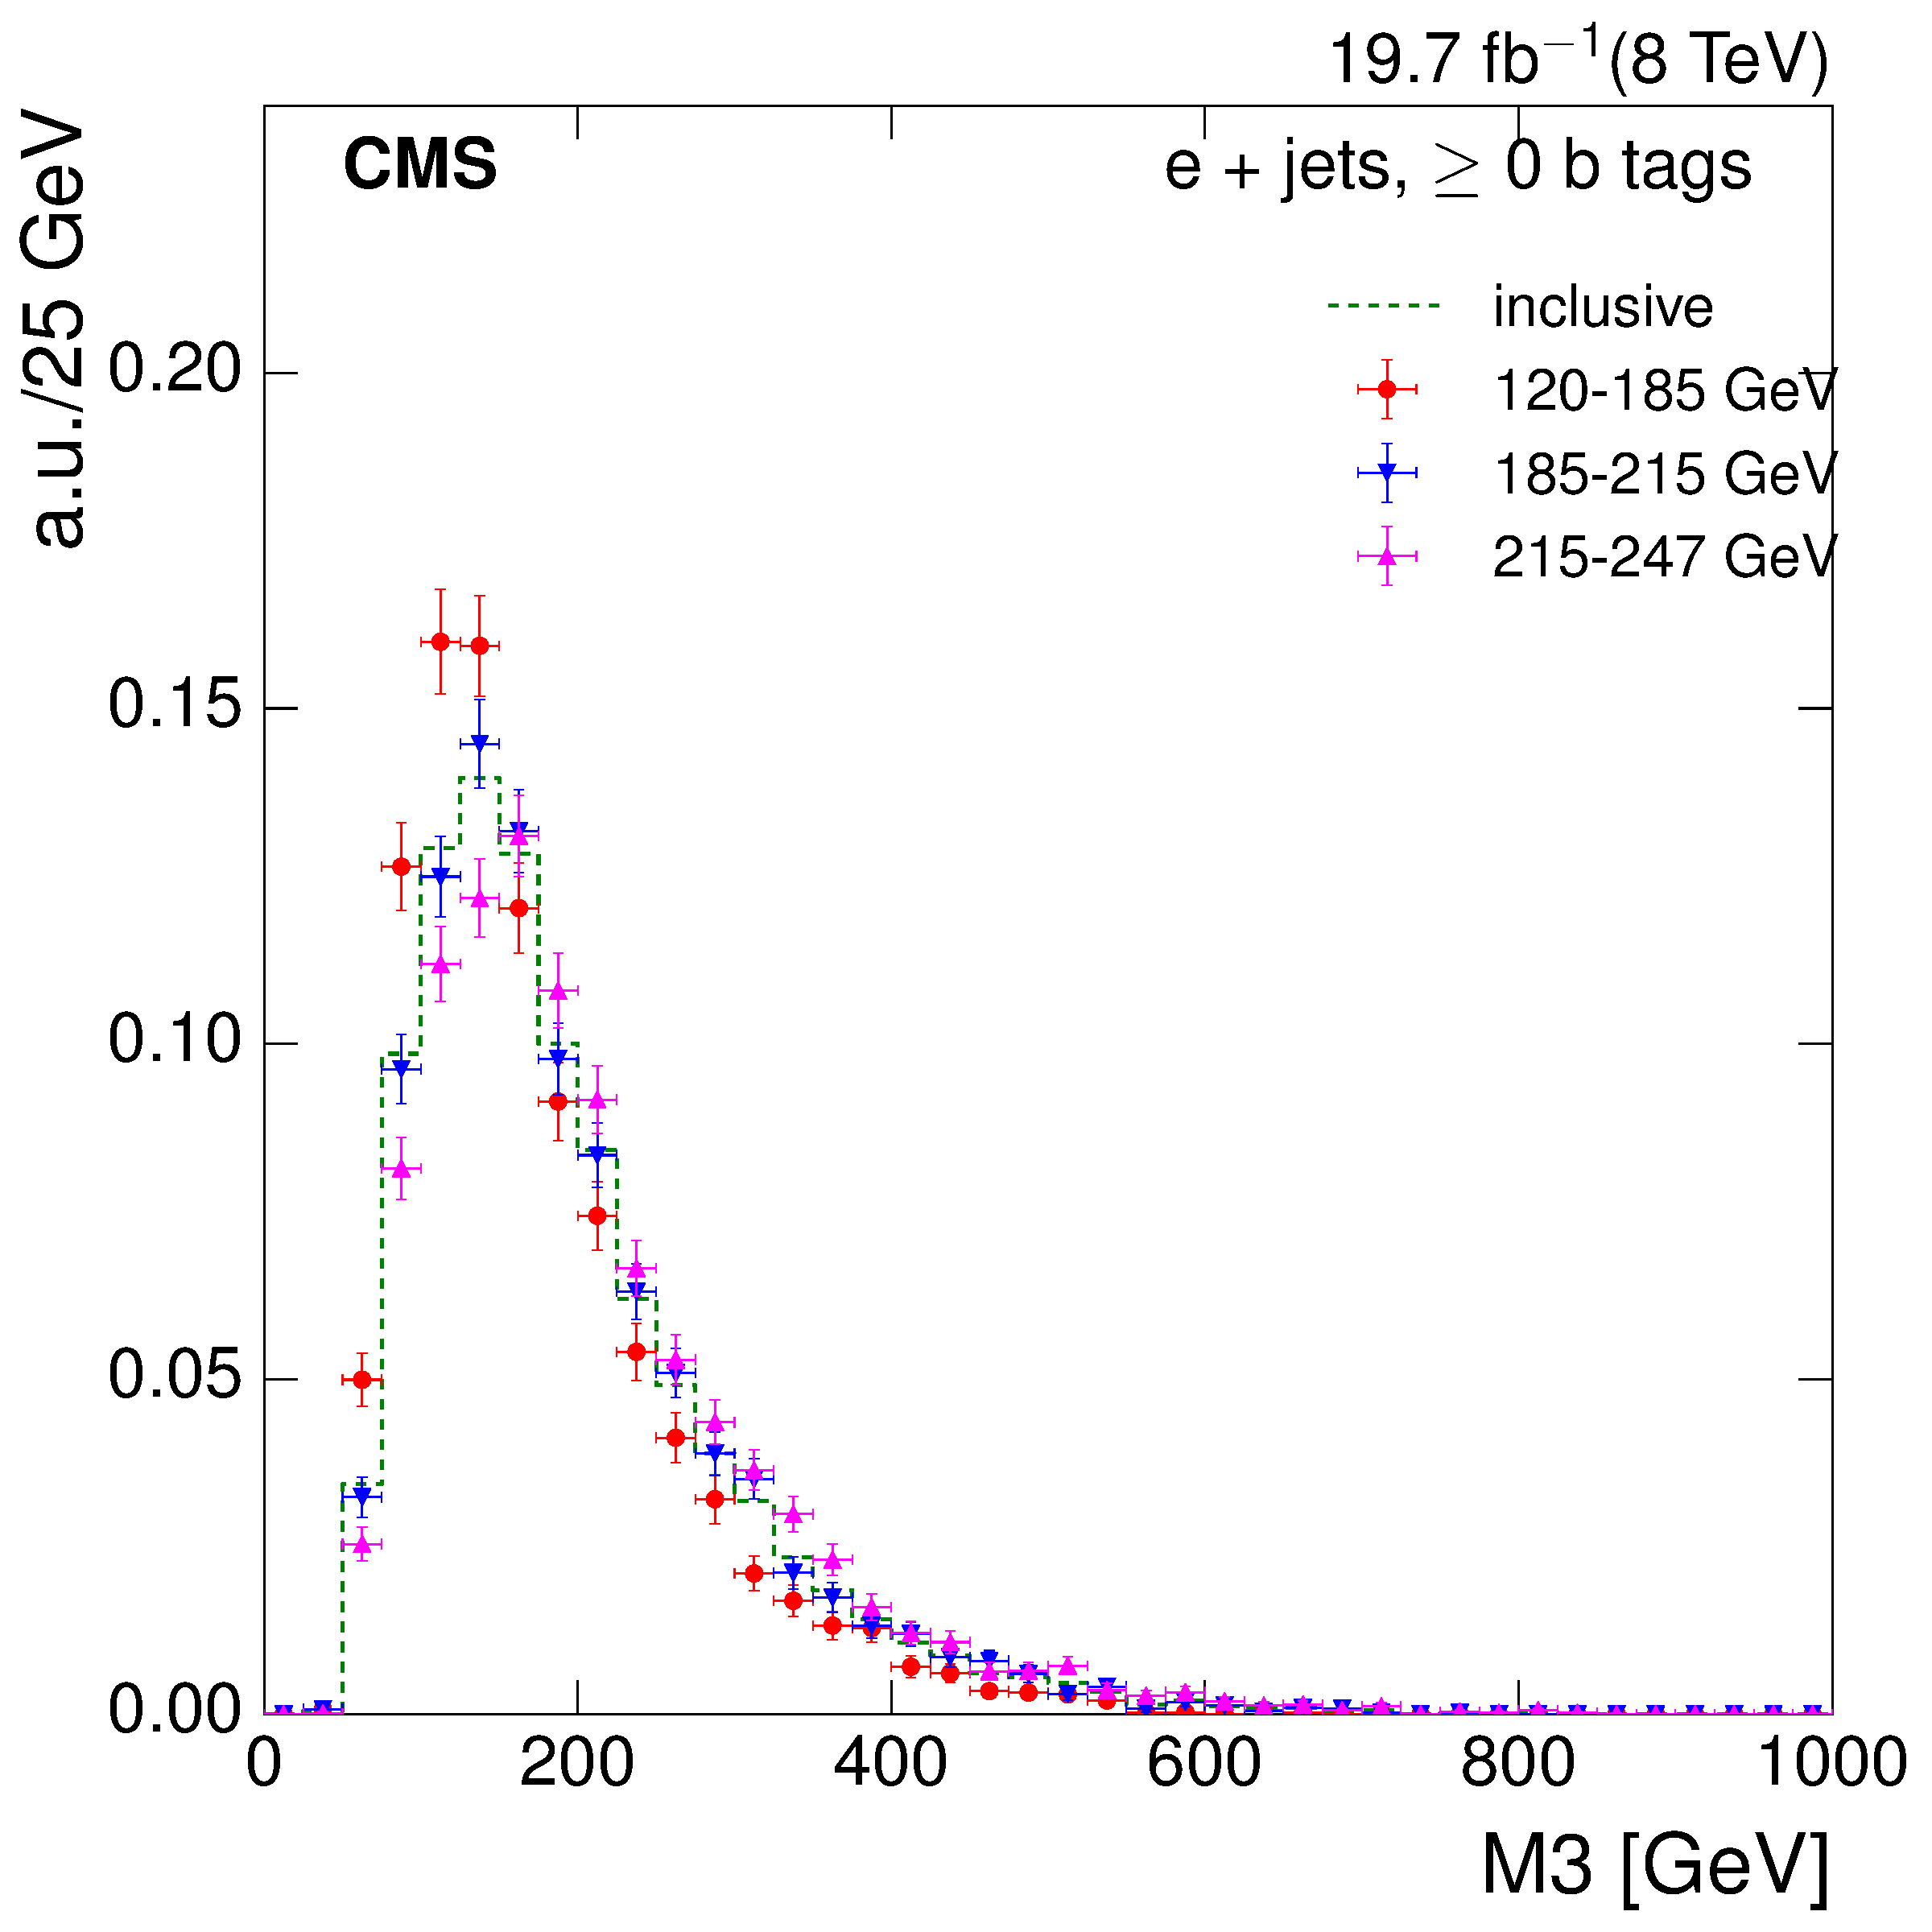
\includegraphics[width=0.48\textwidth]{Chapters/07_08_09_Analysis/Images/8TeV/fit_variables/electron/HT/M3/qcd/HT_M3_0orMoreBtag_QCD_template_comparison.pdf}\hfill
%      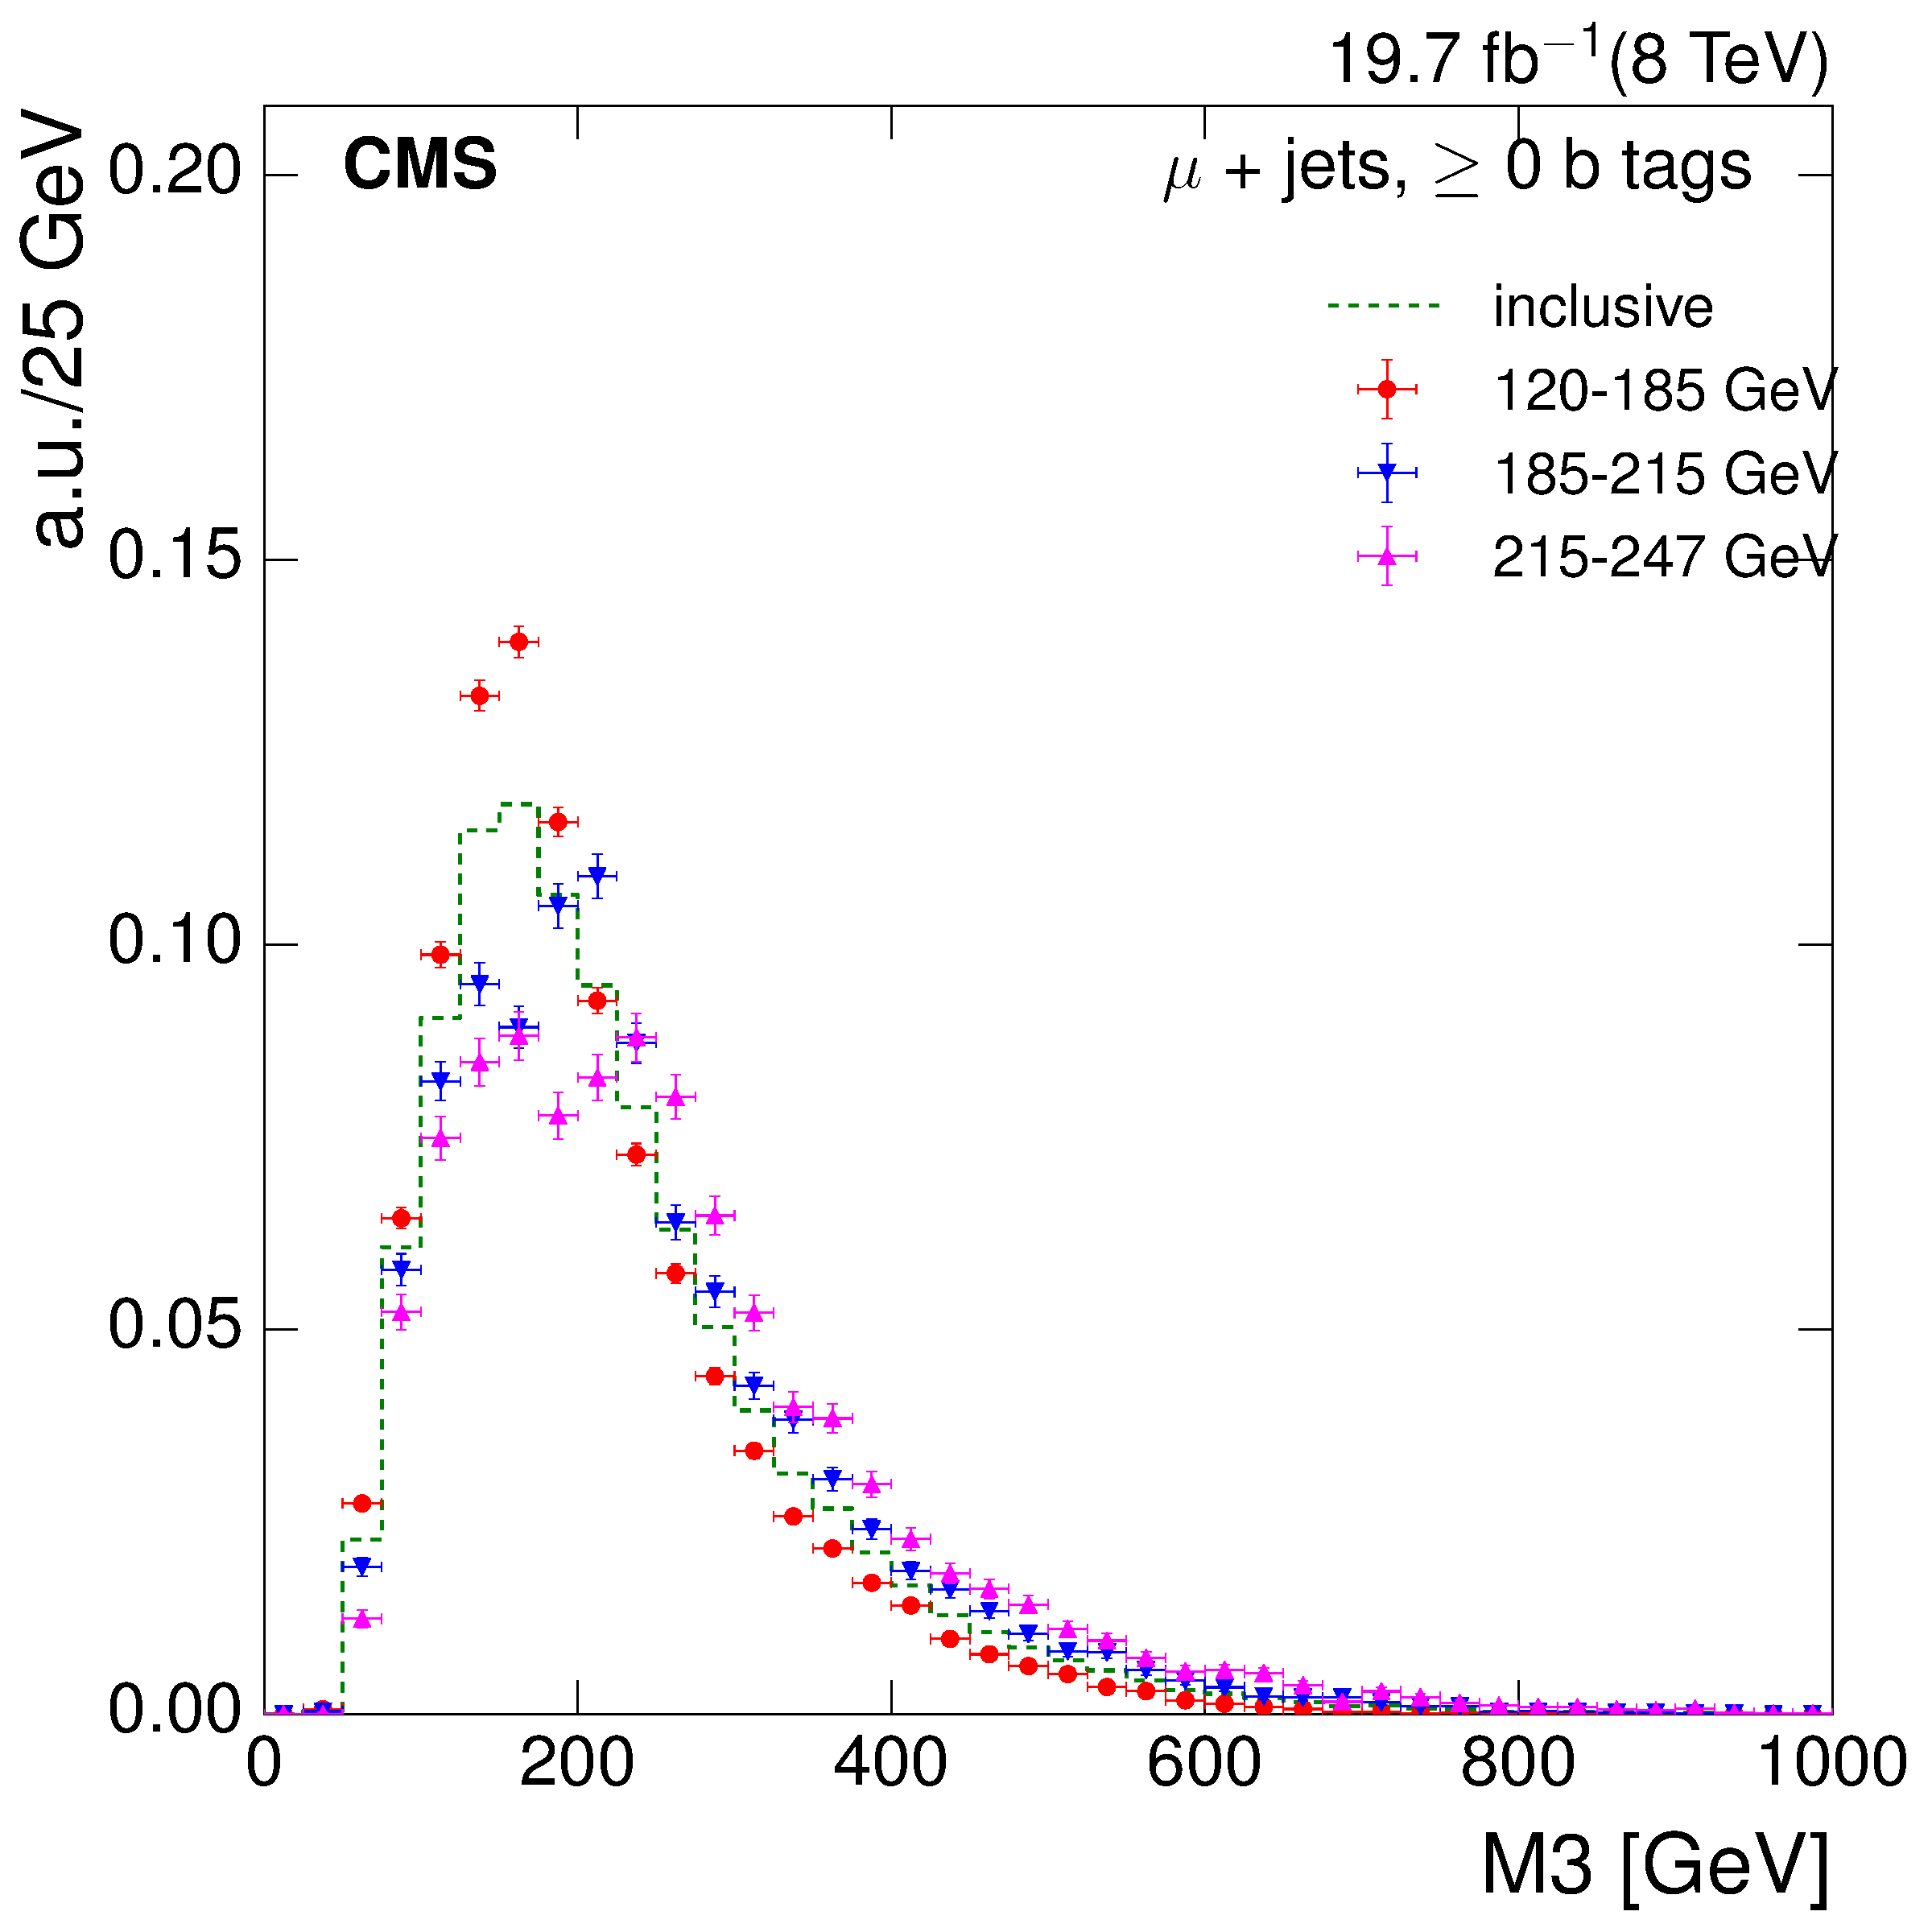
\includegraphics[width=0.48\textwidth]{Chapters/07_08_09_Analysis/Images/8TeV/fit_variables/muon/HT/M3/qcd/HT_M3_0orMoreBtag_QCD_template_comparison.pdf}\\
% 	 \caption[Normalised distributions of the QCD templates for the three fit variables in \HT bins at
% 	 $\sqrt{s}=8\TeV$.]{Normalised distributions of the QCD templates for the three fit variables lepton \abseta
% 	 (upper), $\alpha$ (middle) and M3 (lower) inclusive across all \HT bins and for the lowest three \HT bins at
% 	 $\sqrt{s}=8\TeV$ in the electron+jets channel (left) and in the muon+jets channel (right).}
%      \label{fig:HT_fit_variable_qcd_comparisons_8TeV}
% \end{figure}
% 
% \begin{figure}[hbtp]
%     \centering
%      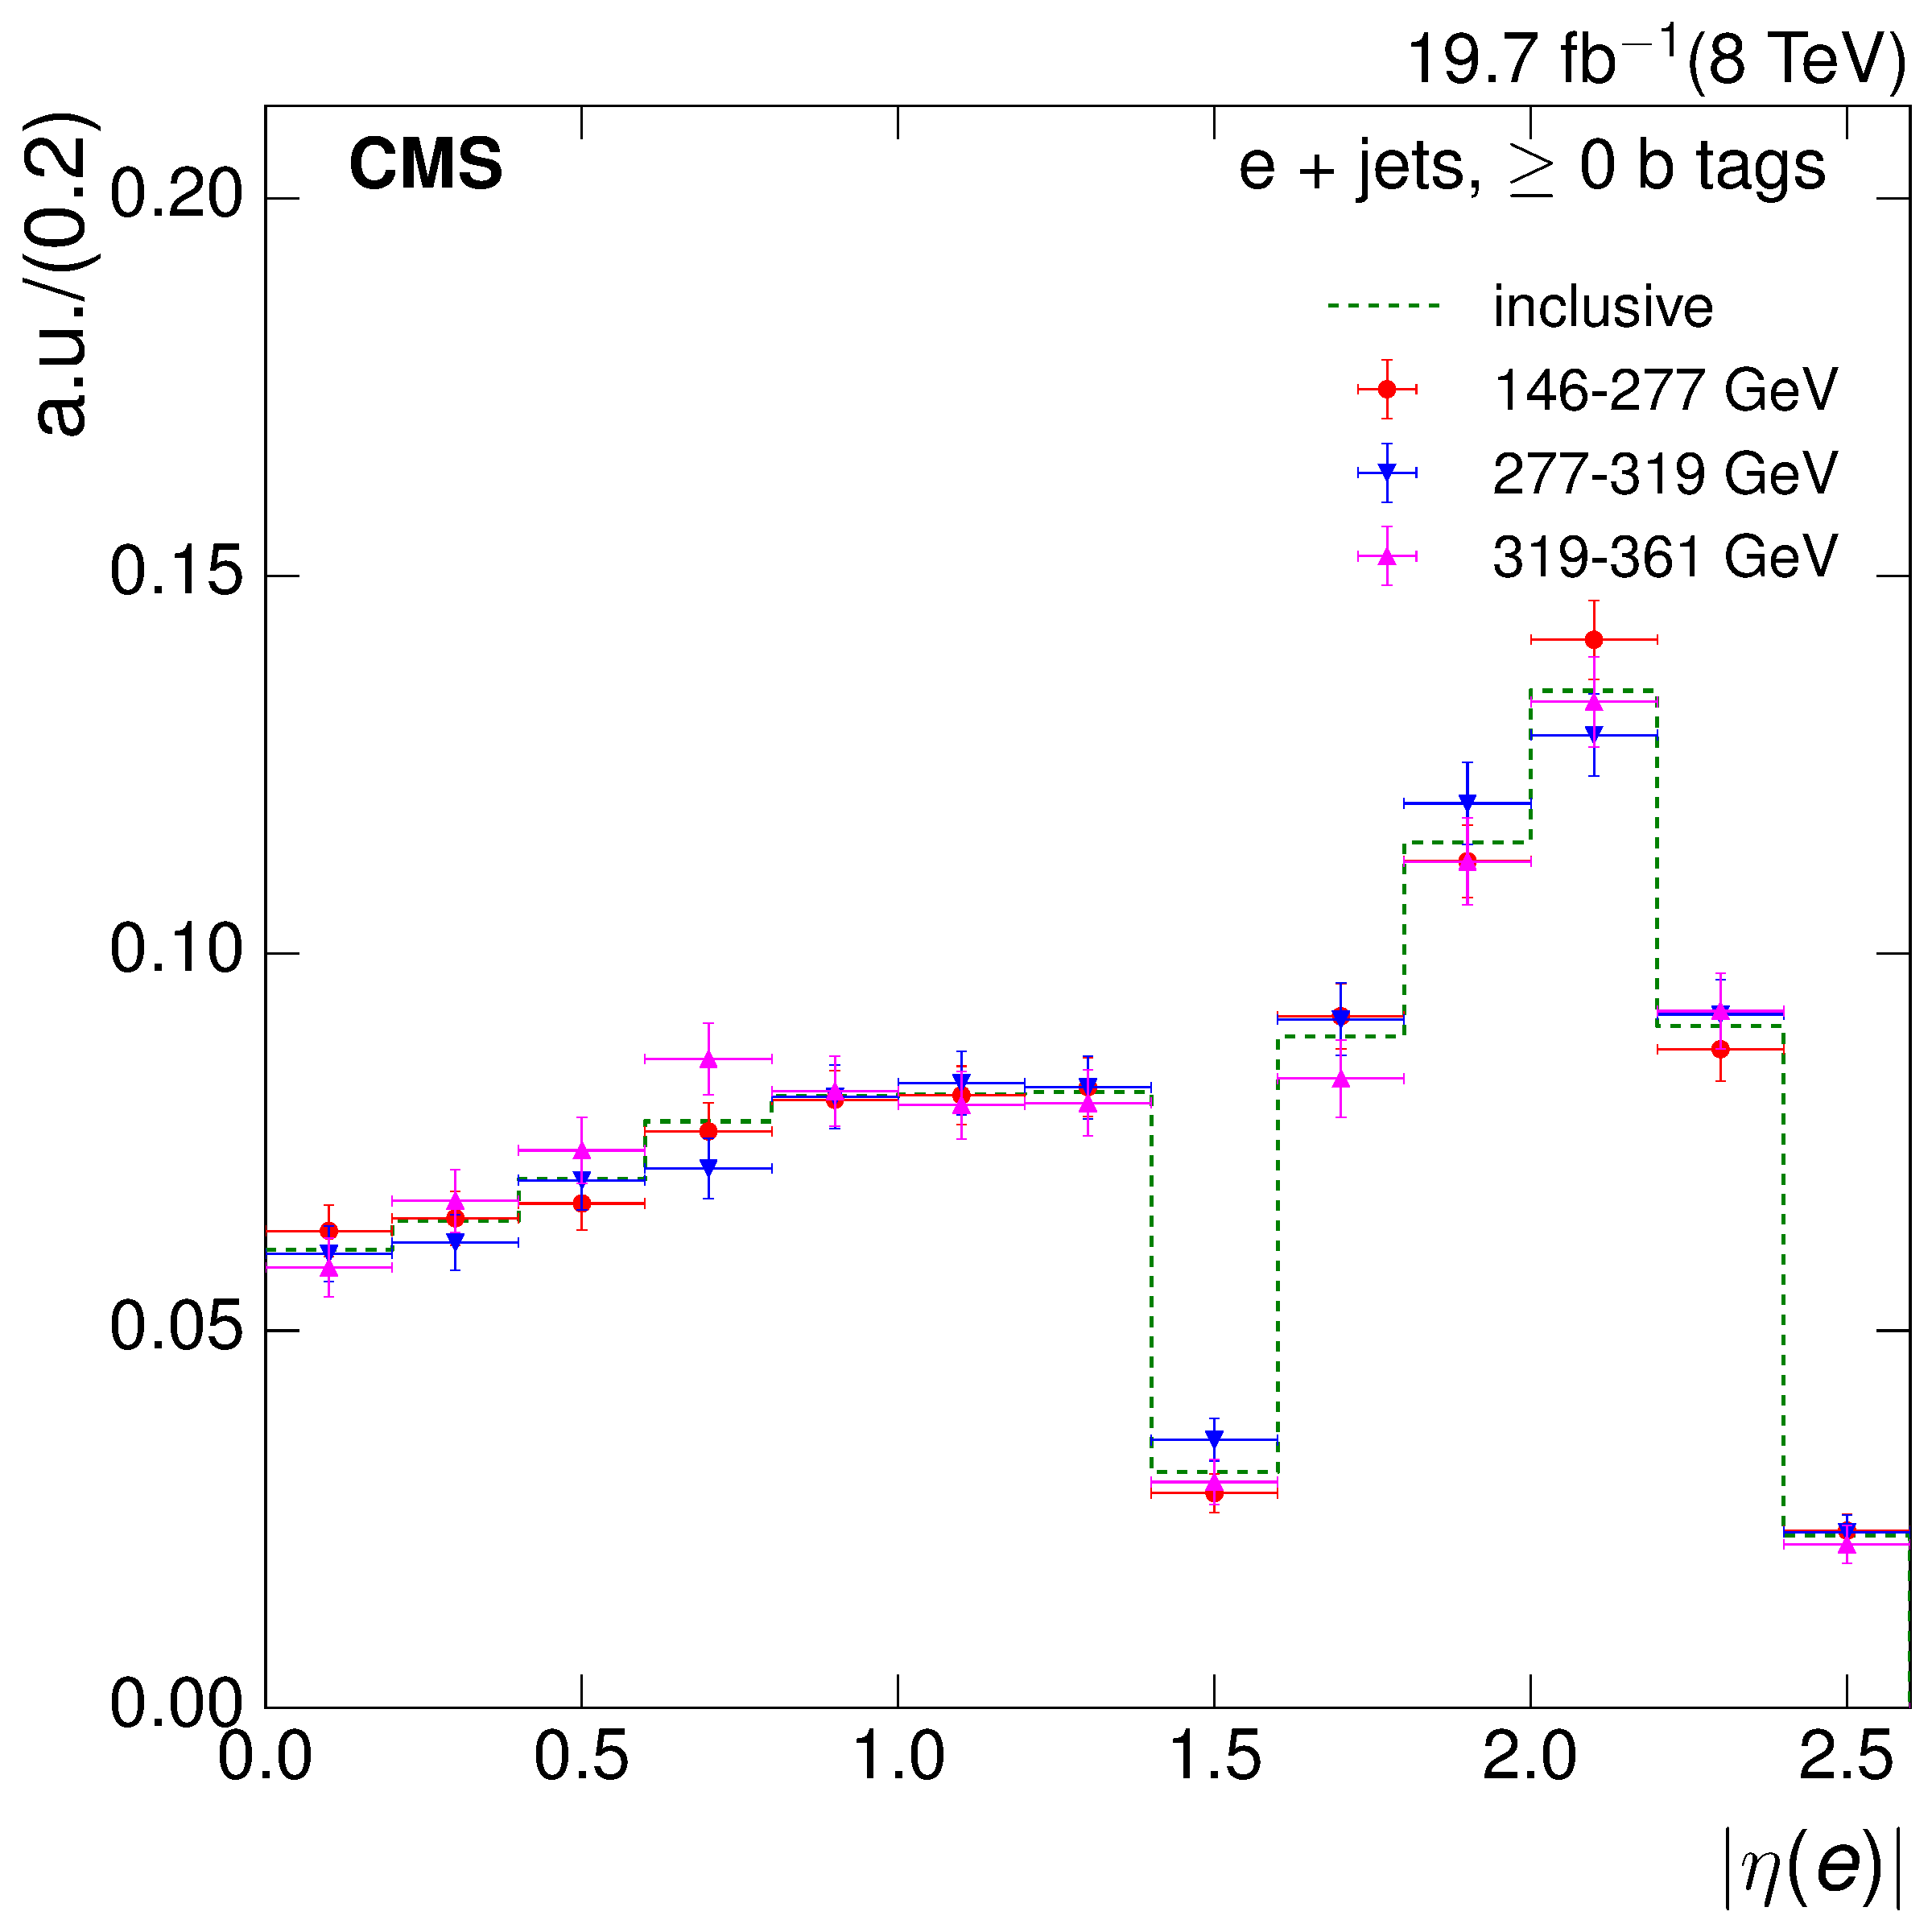
\includegraphics[width=0.48\textwidth]{Chapters/07_08_09_Analysis/Images/8TeV/fit_variables/electron/ST/electron_absolute_eta/qcd/ST_electron_absolute_eta_0orMoreBtag_QCD_template_comparison.pdf}\hfill
%      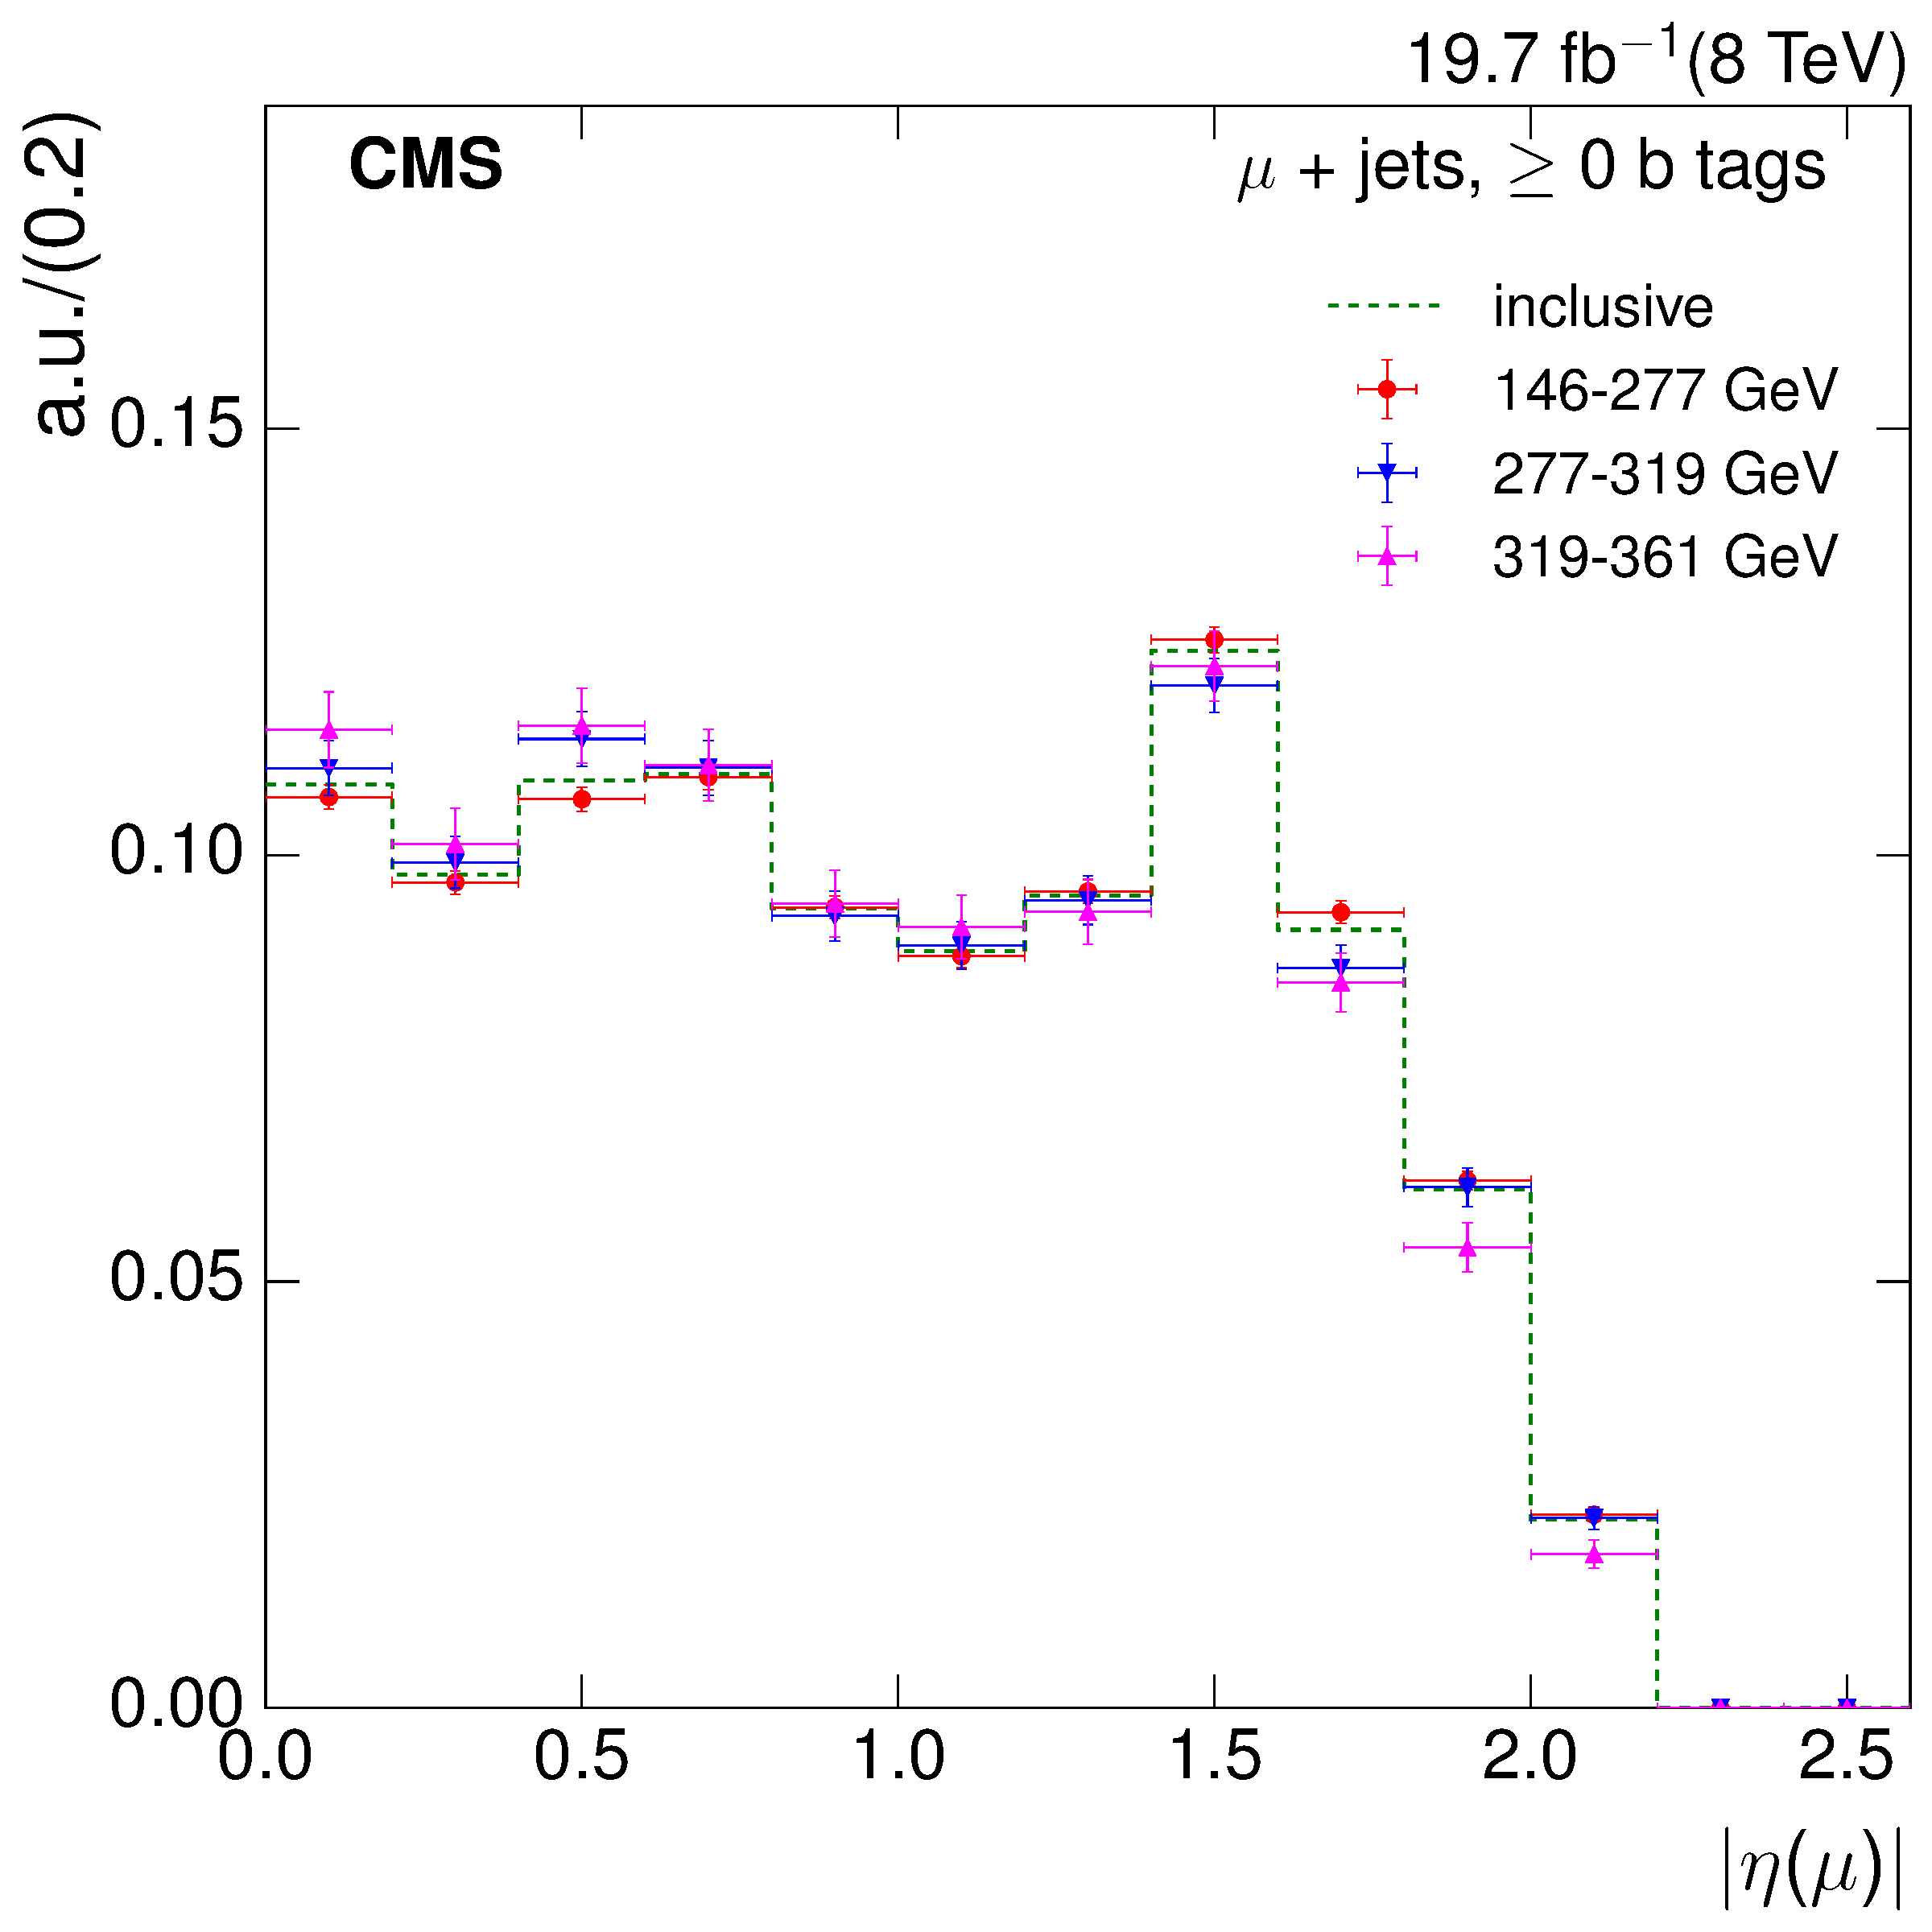
\includegraphics[width=0.48\textwidth]{Chapters/07_08_09_Analysis/Images/8TeV/fit_variables/muon/ST/muon_absolute_eta/qcd/ST_muon_absolute_eta_0orMoreBtag_QCD_template_comparison.pdf}\\
%      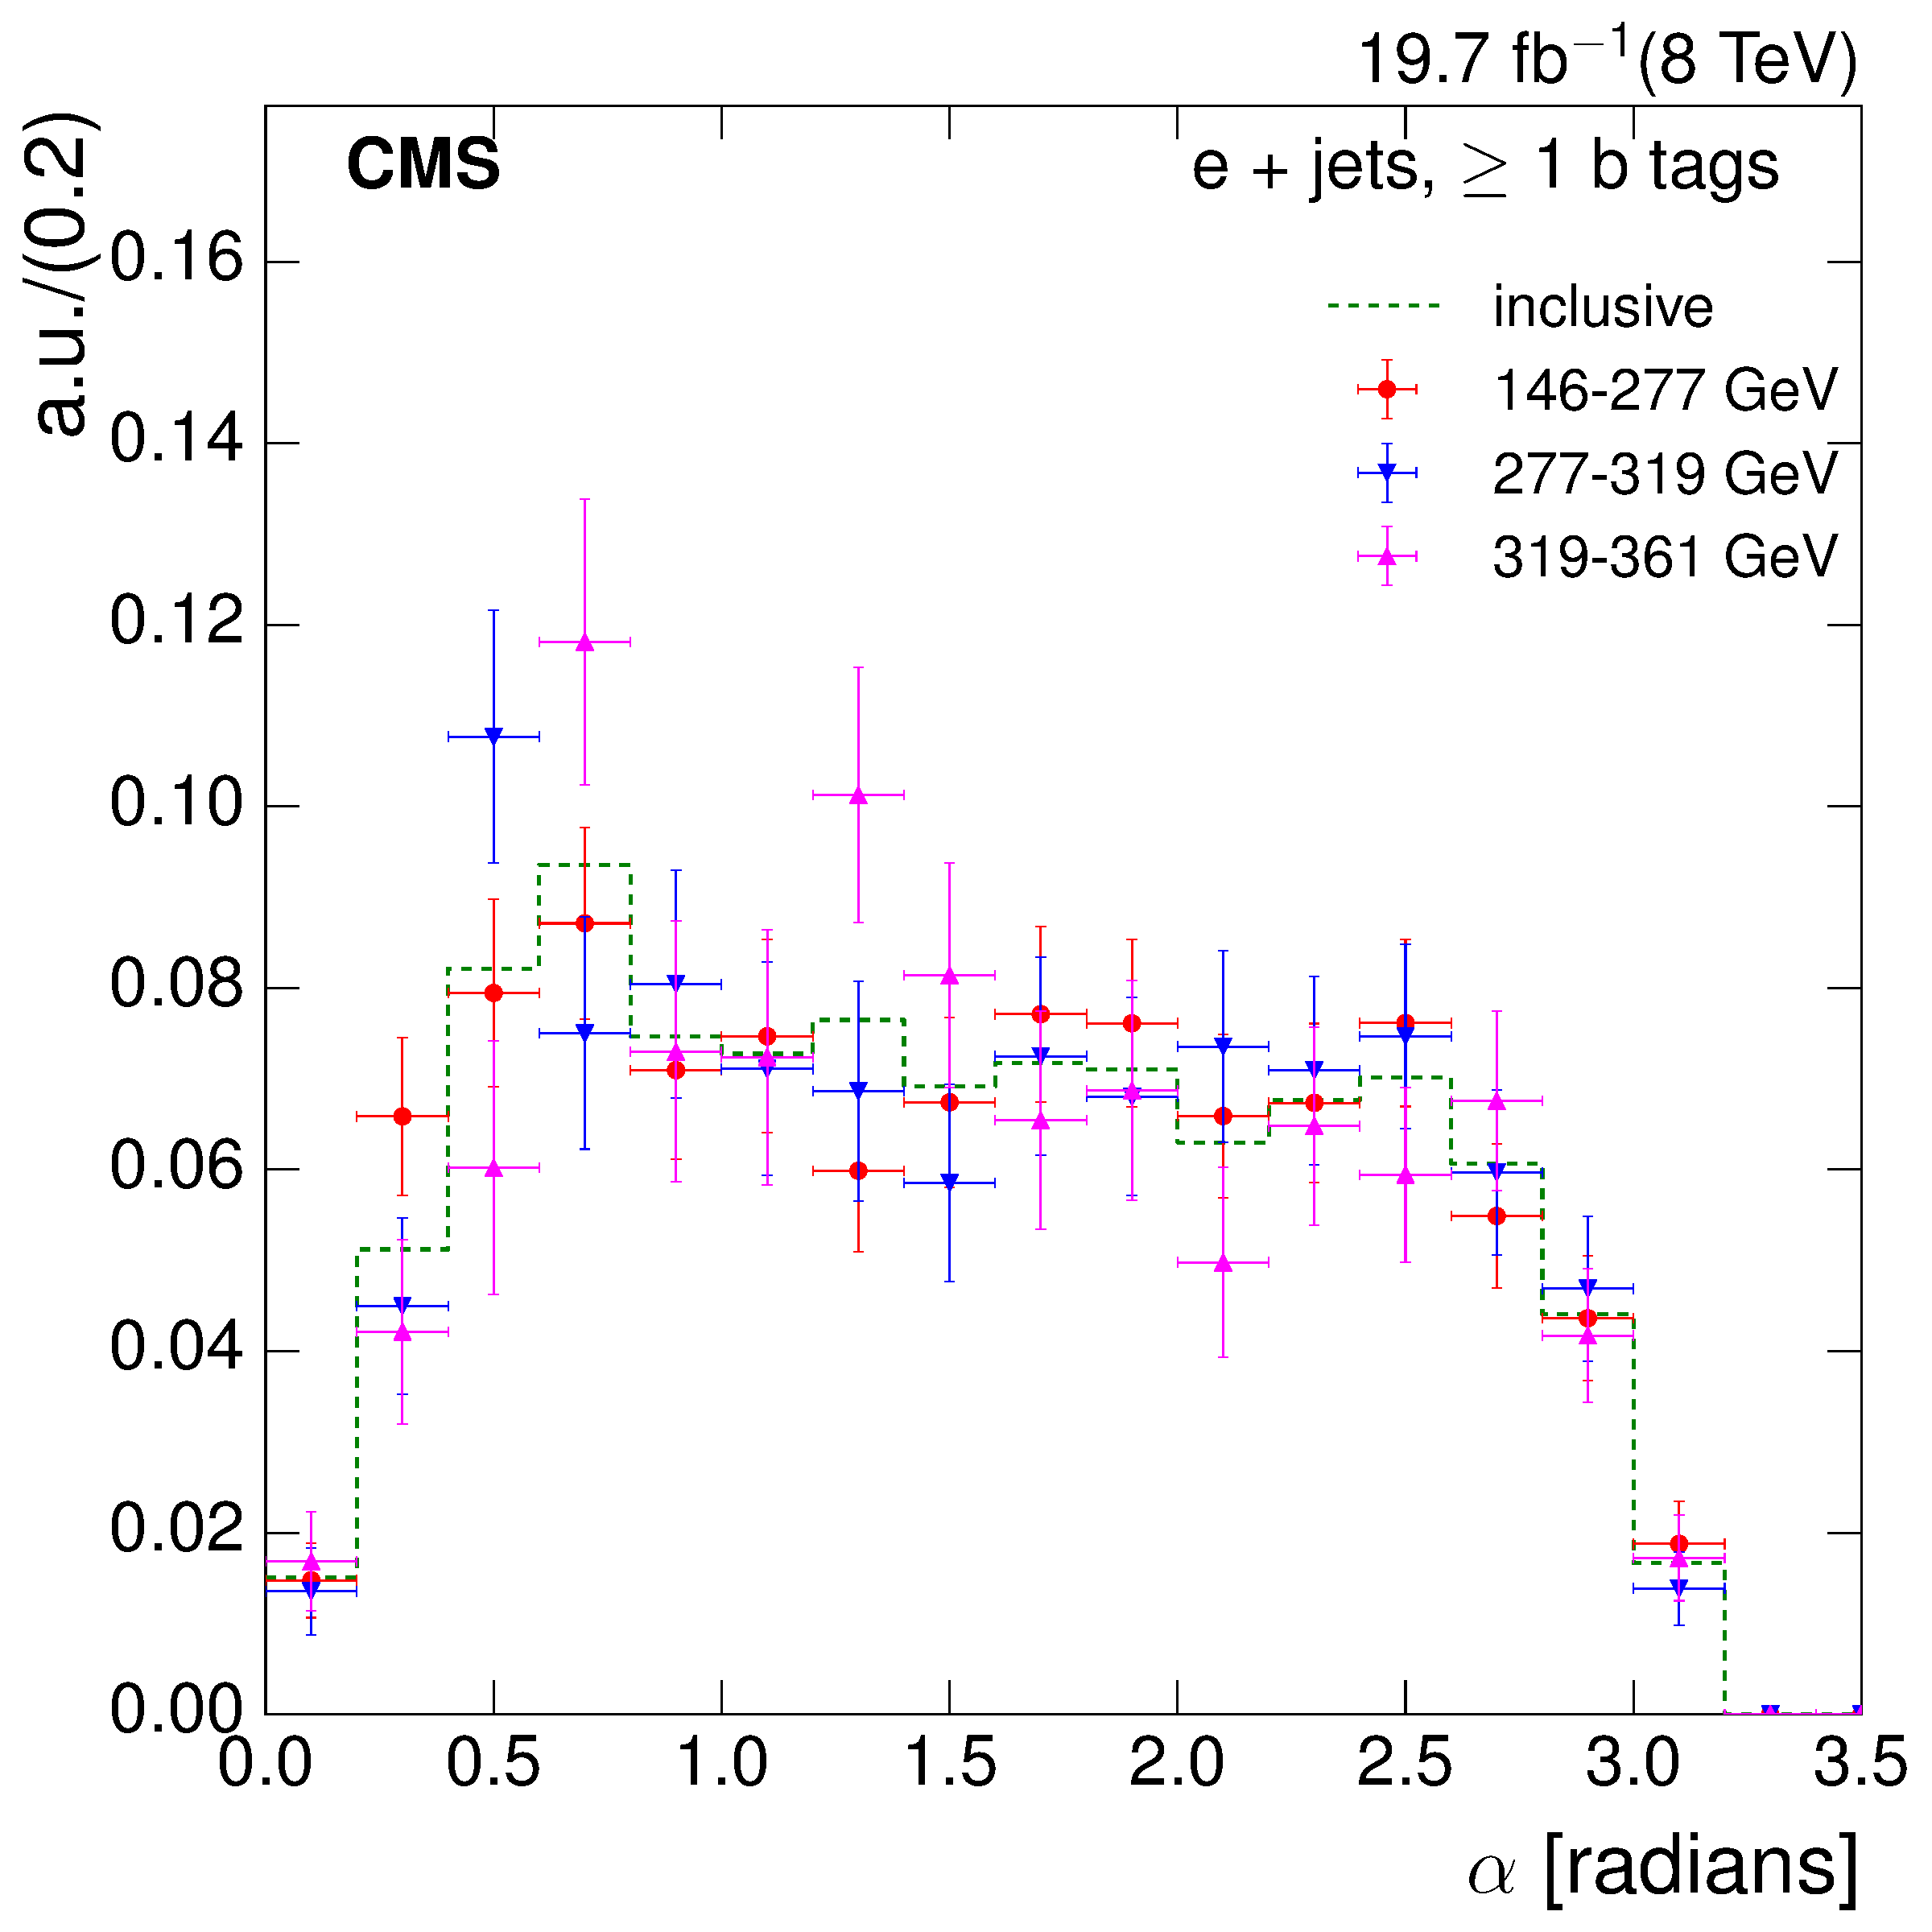
\includegraphics[width=0.48\textwidth]{Chapters/07_08_09_Analysis/Images/8TeV/fit_variables/electron/ST/angle_bl/qcd/ST_angle_bl_1orMoreBtag_QCD_template_comparison.pdf}\hfill
%      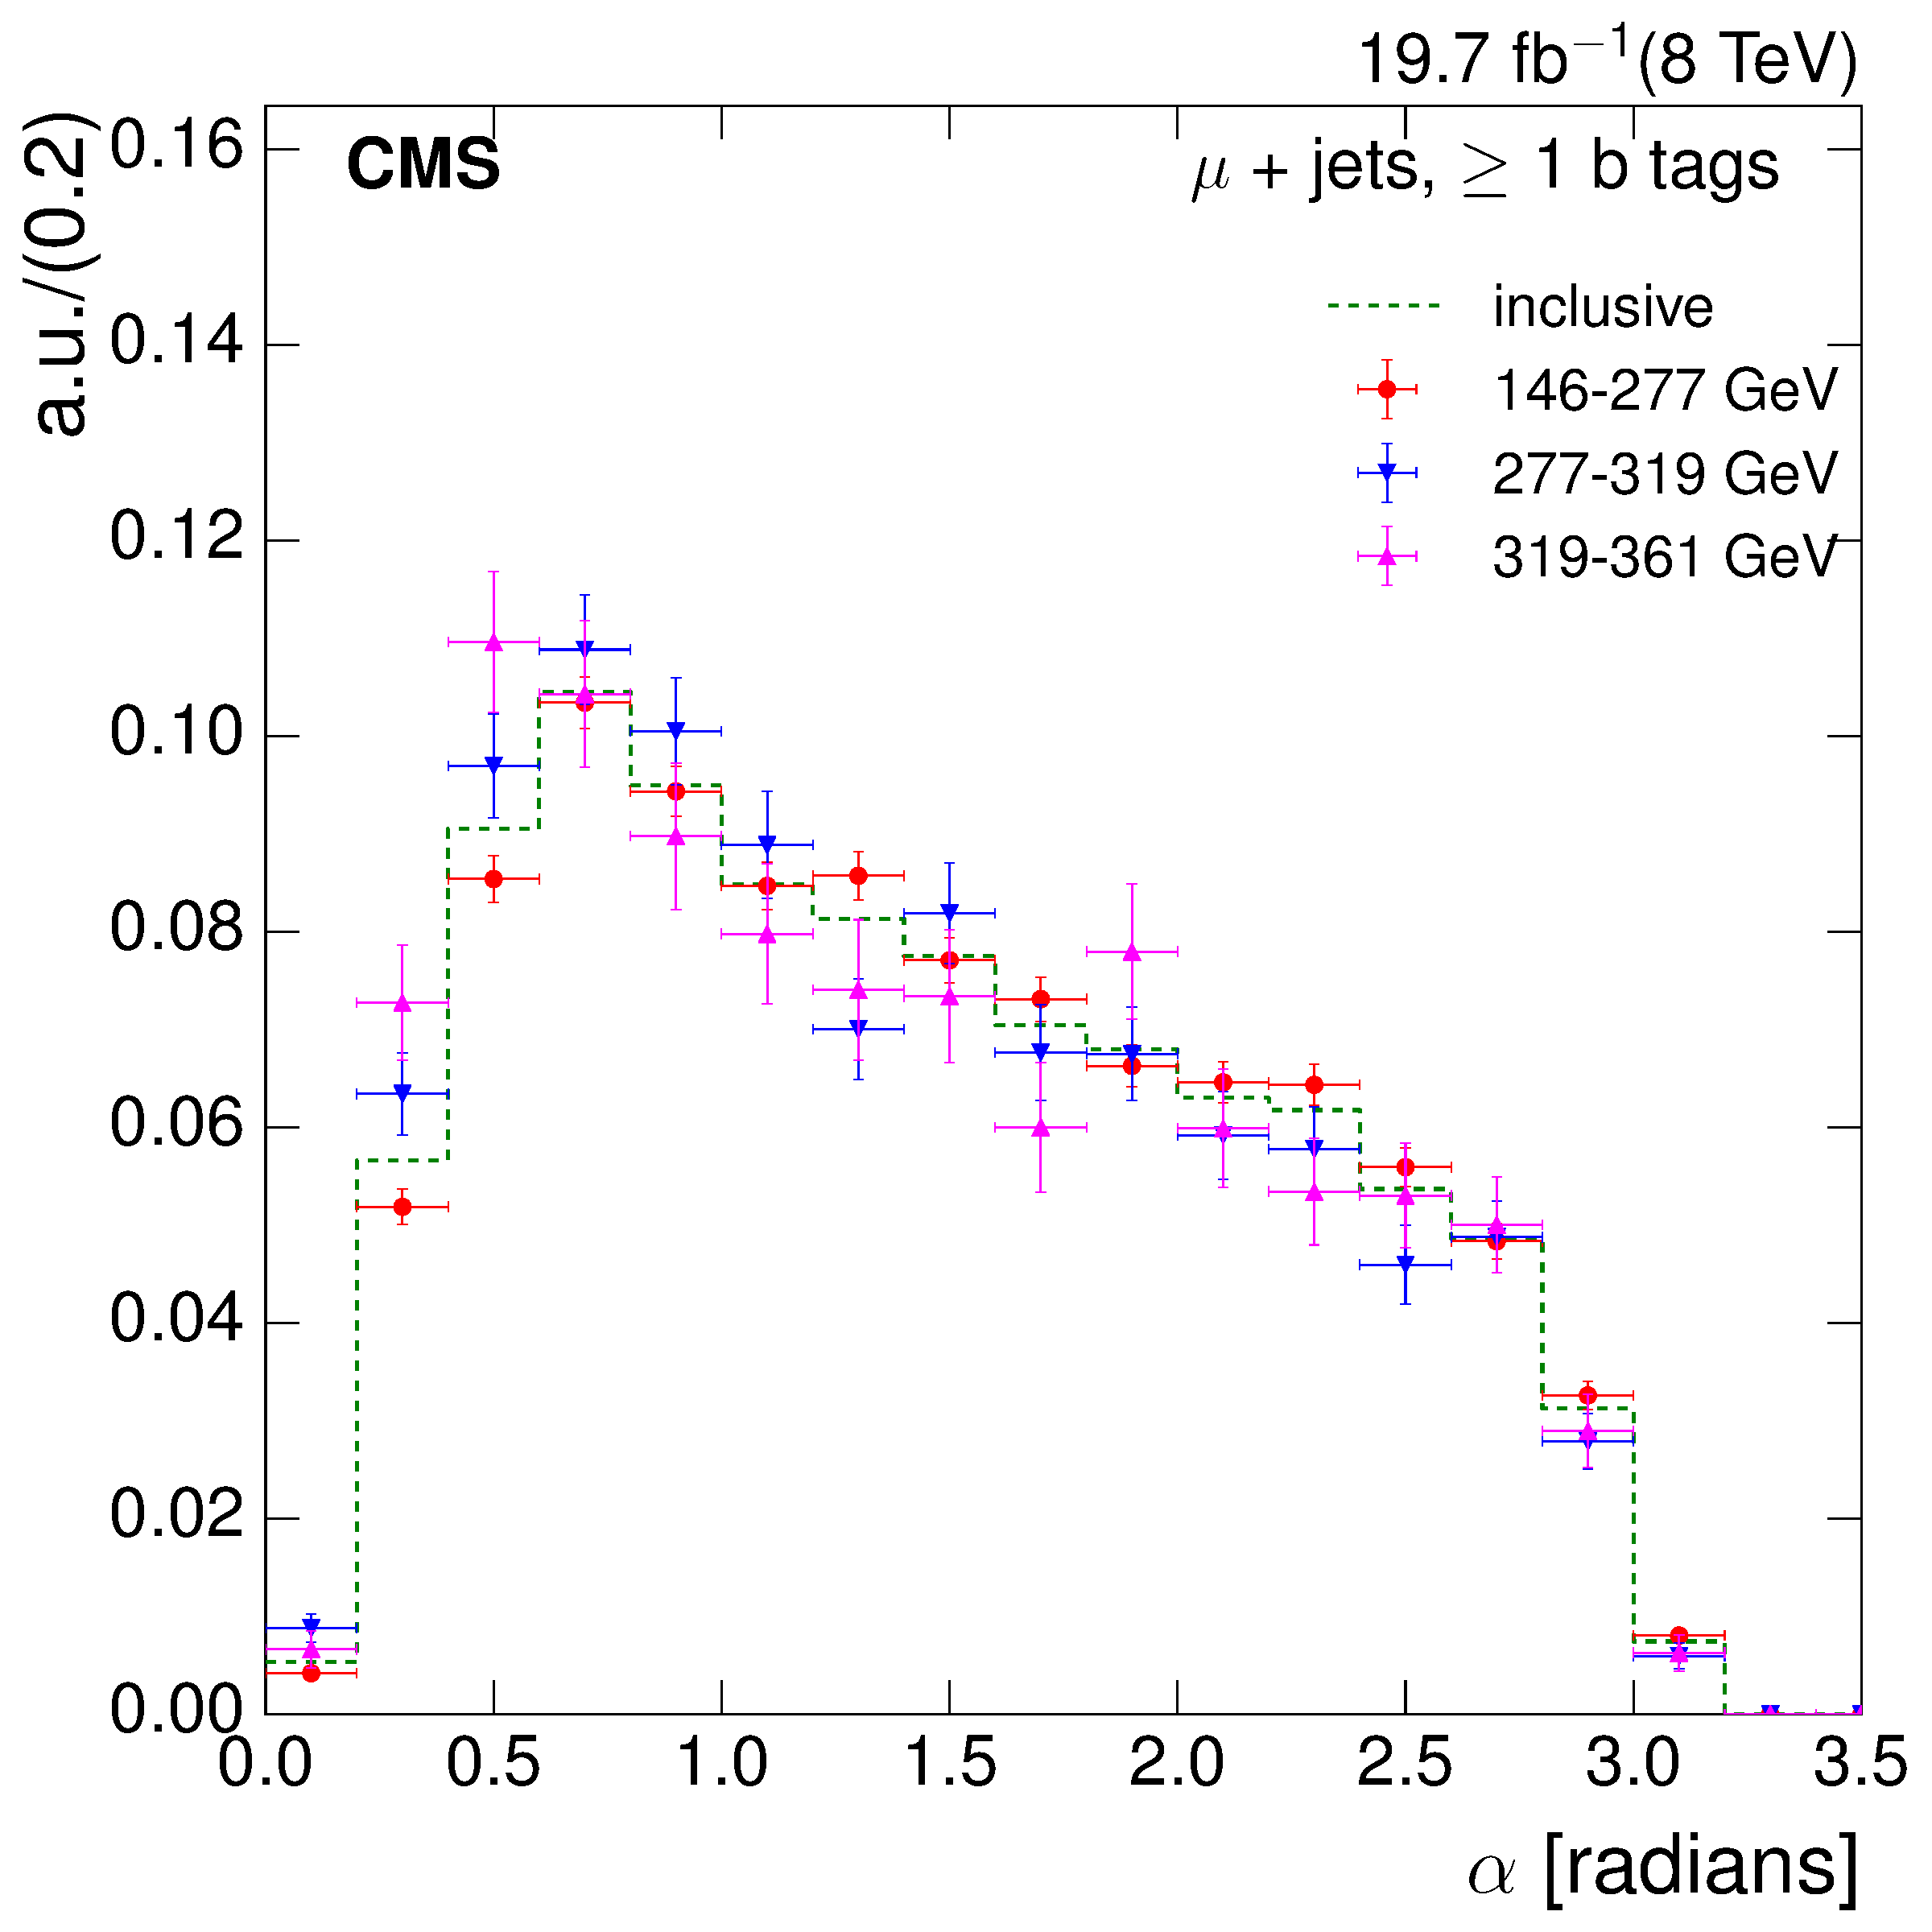
\includegraphics[width=0.48\textwidth]{Chapters/07_08_09_Analysis/Images/8TeV/fit_variables/muon/ST/angle_bl/qcd/ST_angle_bl_1orMoreBtag_QCD_template_comparison.pdf}\\
%      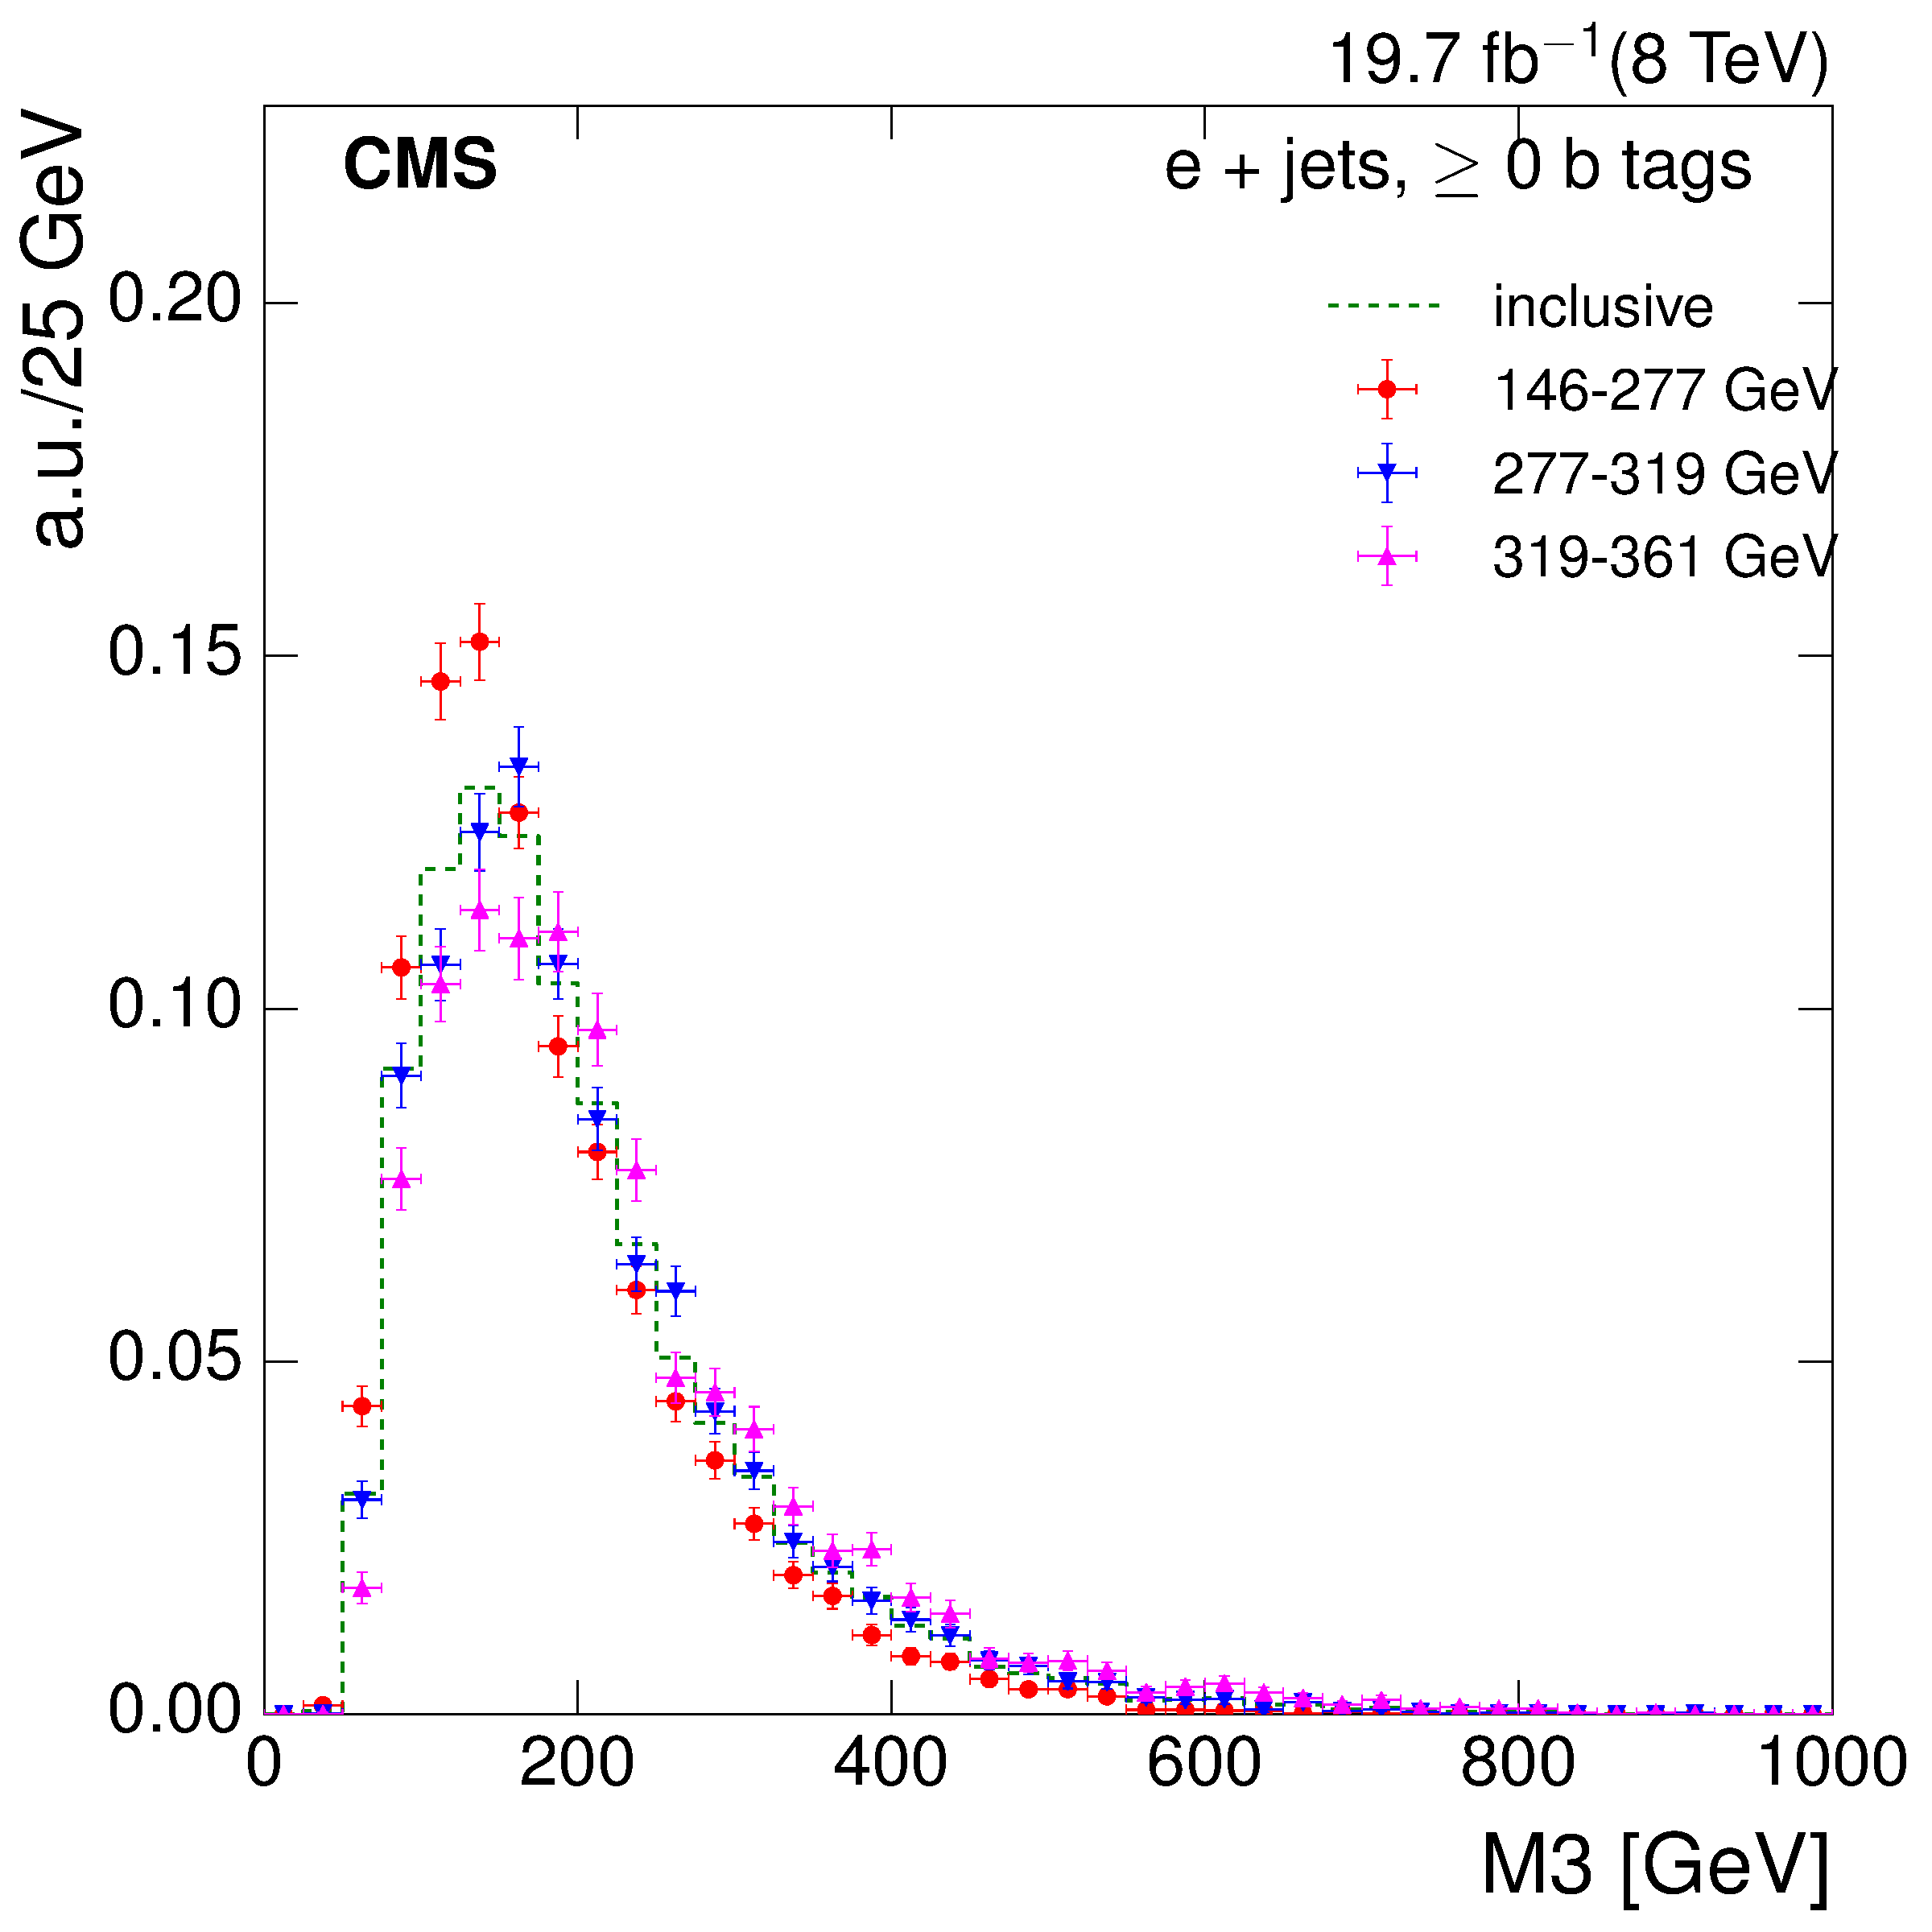
\includegraphics[width=0.48\textwidth]{Chapters/07_08_09_Analysis/Images/8TeV/fit_variables/electron/ST/M3/qcd/ST_M3_0orMoreBtag_QCD_template_comparison.pdf}\hfill
%      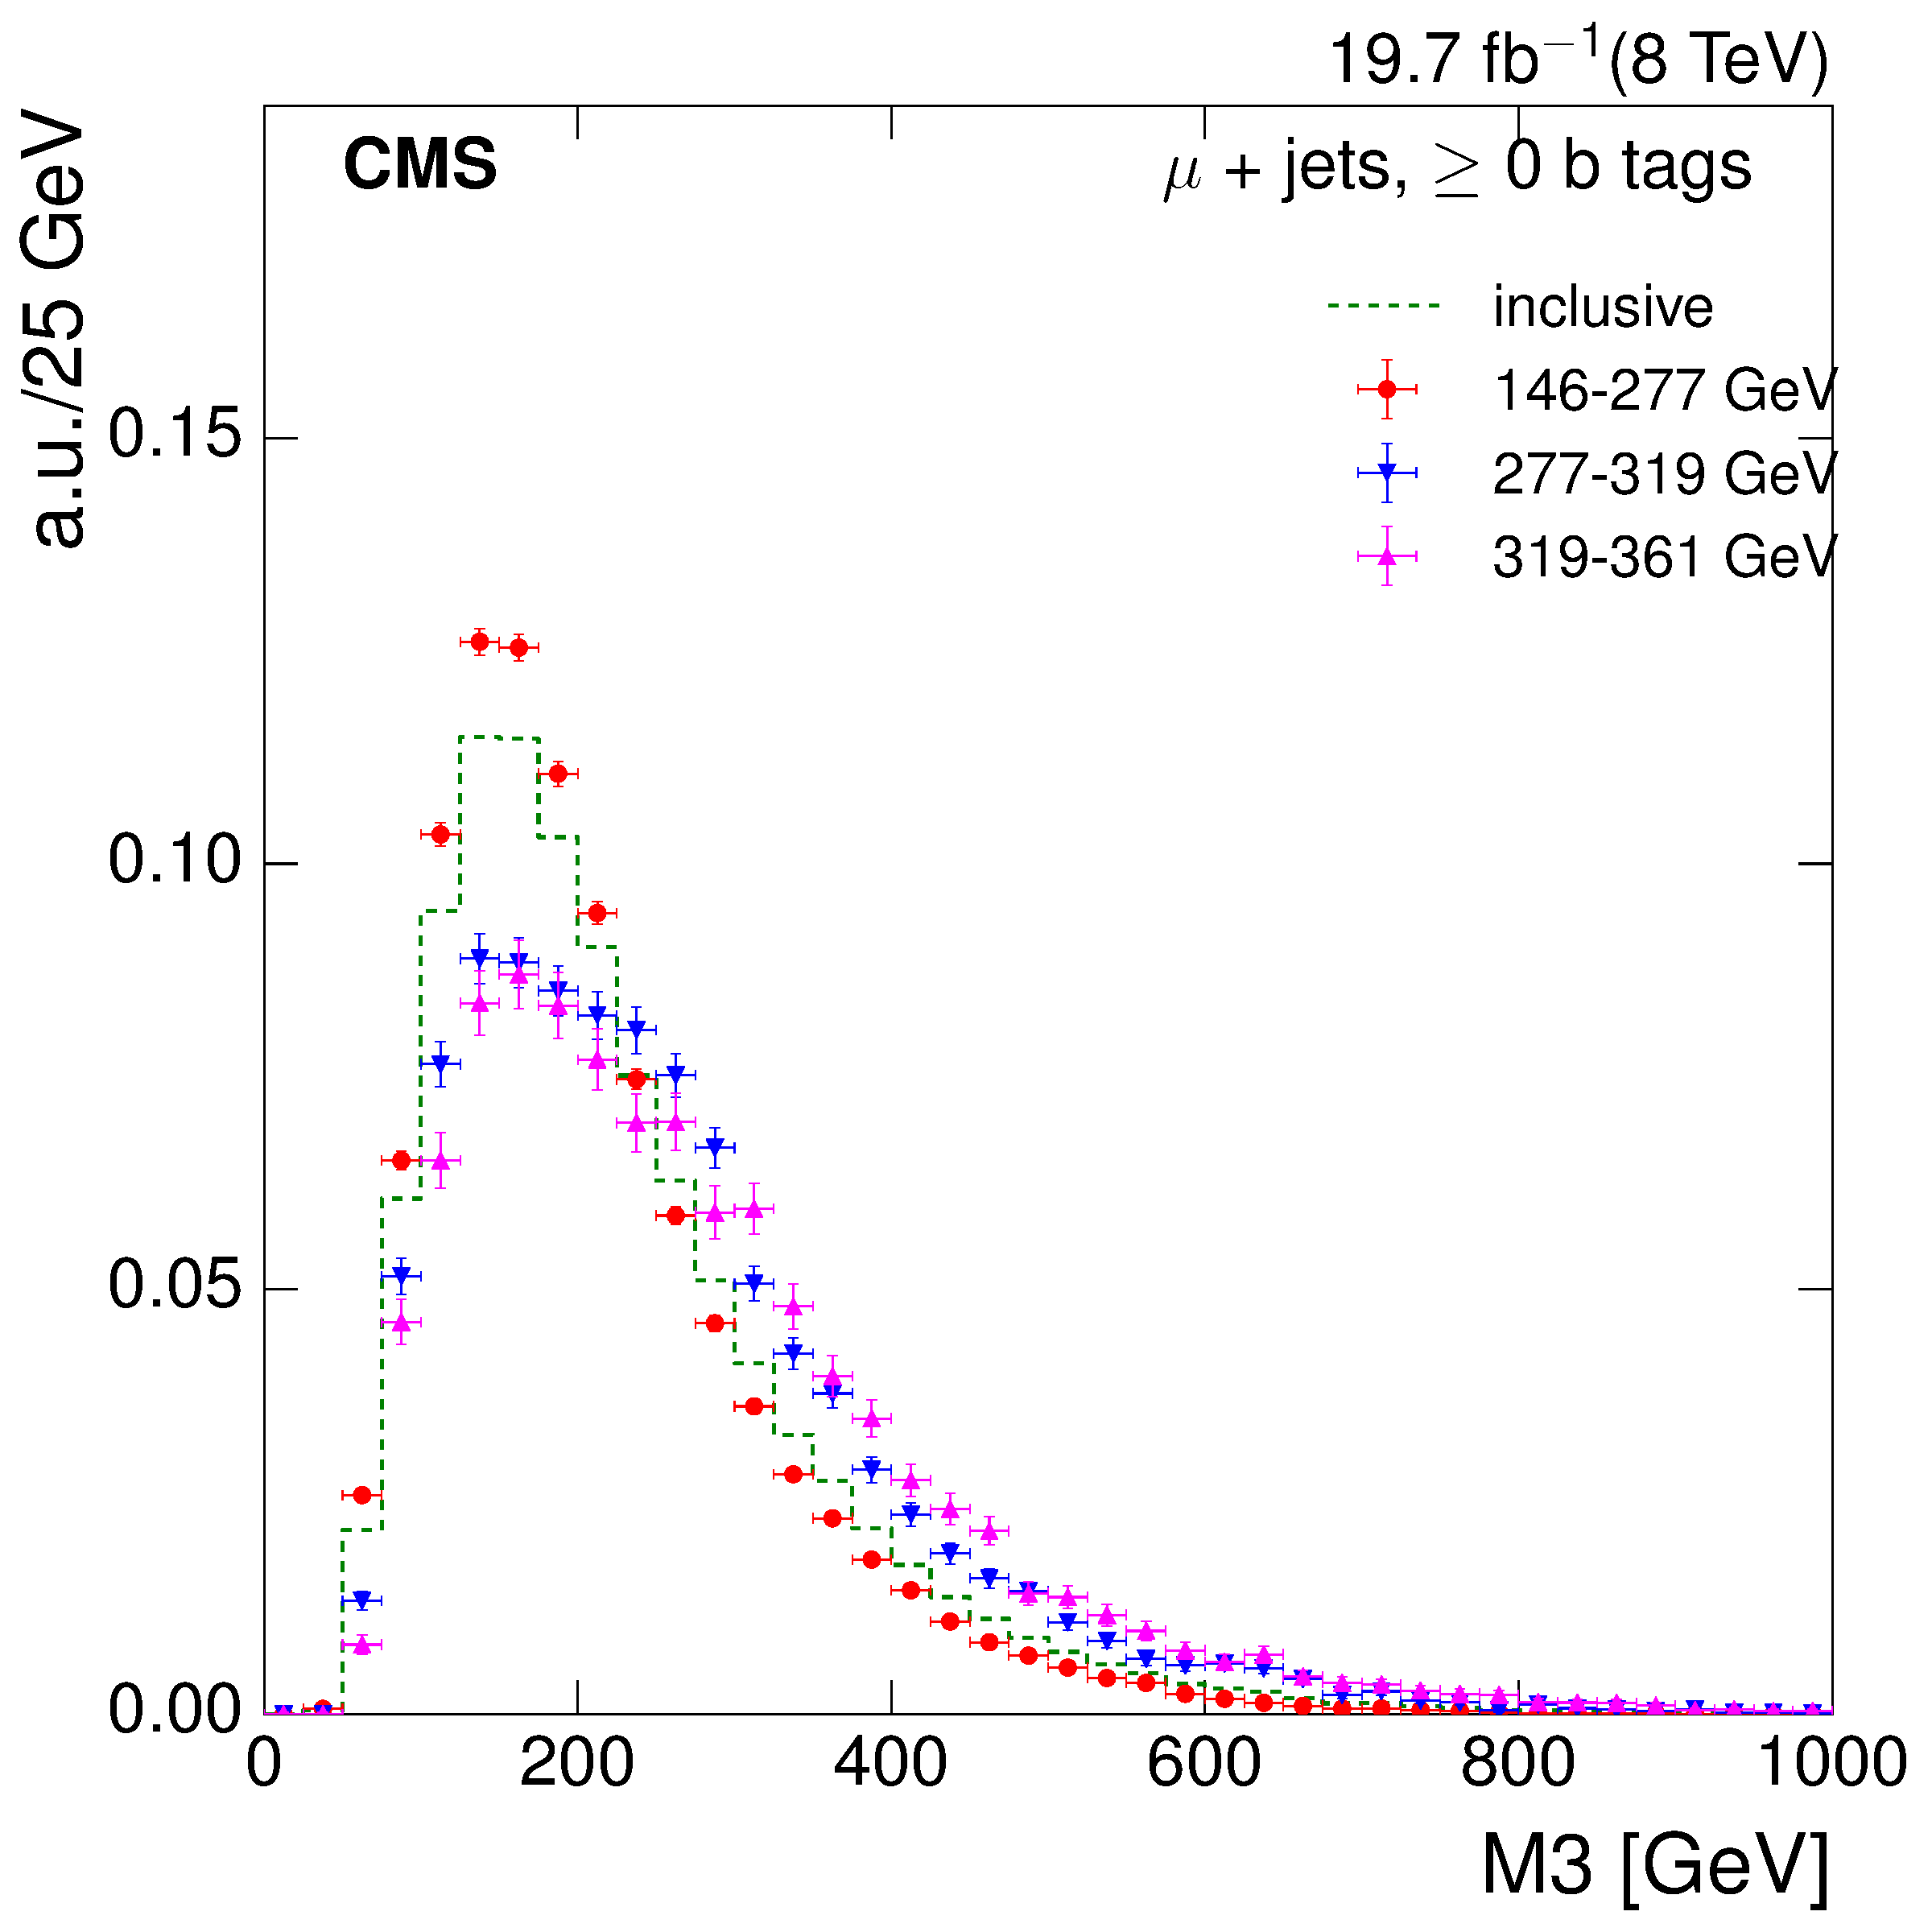
\includegraphics[width=0.48\textwidth]{Chapters/07_08_09_Analysis/Images/8TeV/fit_variables/muon/ST/M3/qcd/ST_M3_0orMoreBtag_QCD_template_comparison.pdf}\\
% 	 \caption[Normalised distributions of the QCD templates for the three fit variables in \st bins
% 	 at $\sqrt{s}=8\TeV$.]{Normalised distributions of the QCD templates for the three fit variables lepton
% 	 \abseta (upper), $\alpha$ (middle) and M3 (lower) inclusive across all \st bins and for the lowest three \st
% 	 bins at $\sqrt{s}=8\TeV$ in the electron+jets channel (left) and in the muon+jets channel (right).}
%      \label{fig:ST_fit_variable_qcd_comparisons_8TeV}
% \end{figure}
% 
% \begin{figure}[hbtp]
%     \centering
%      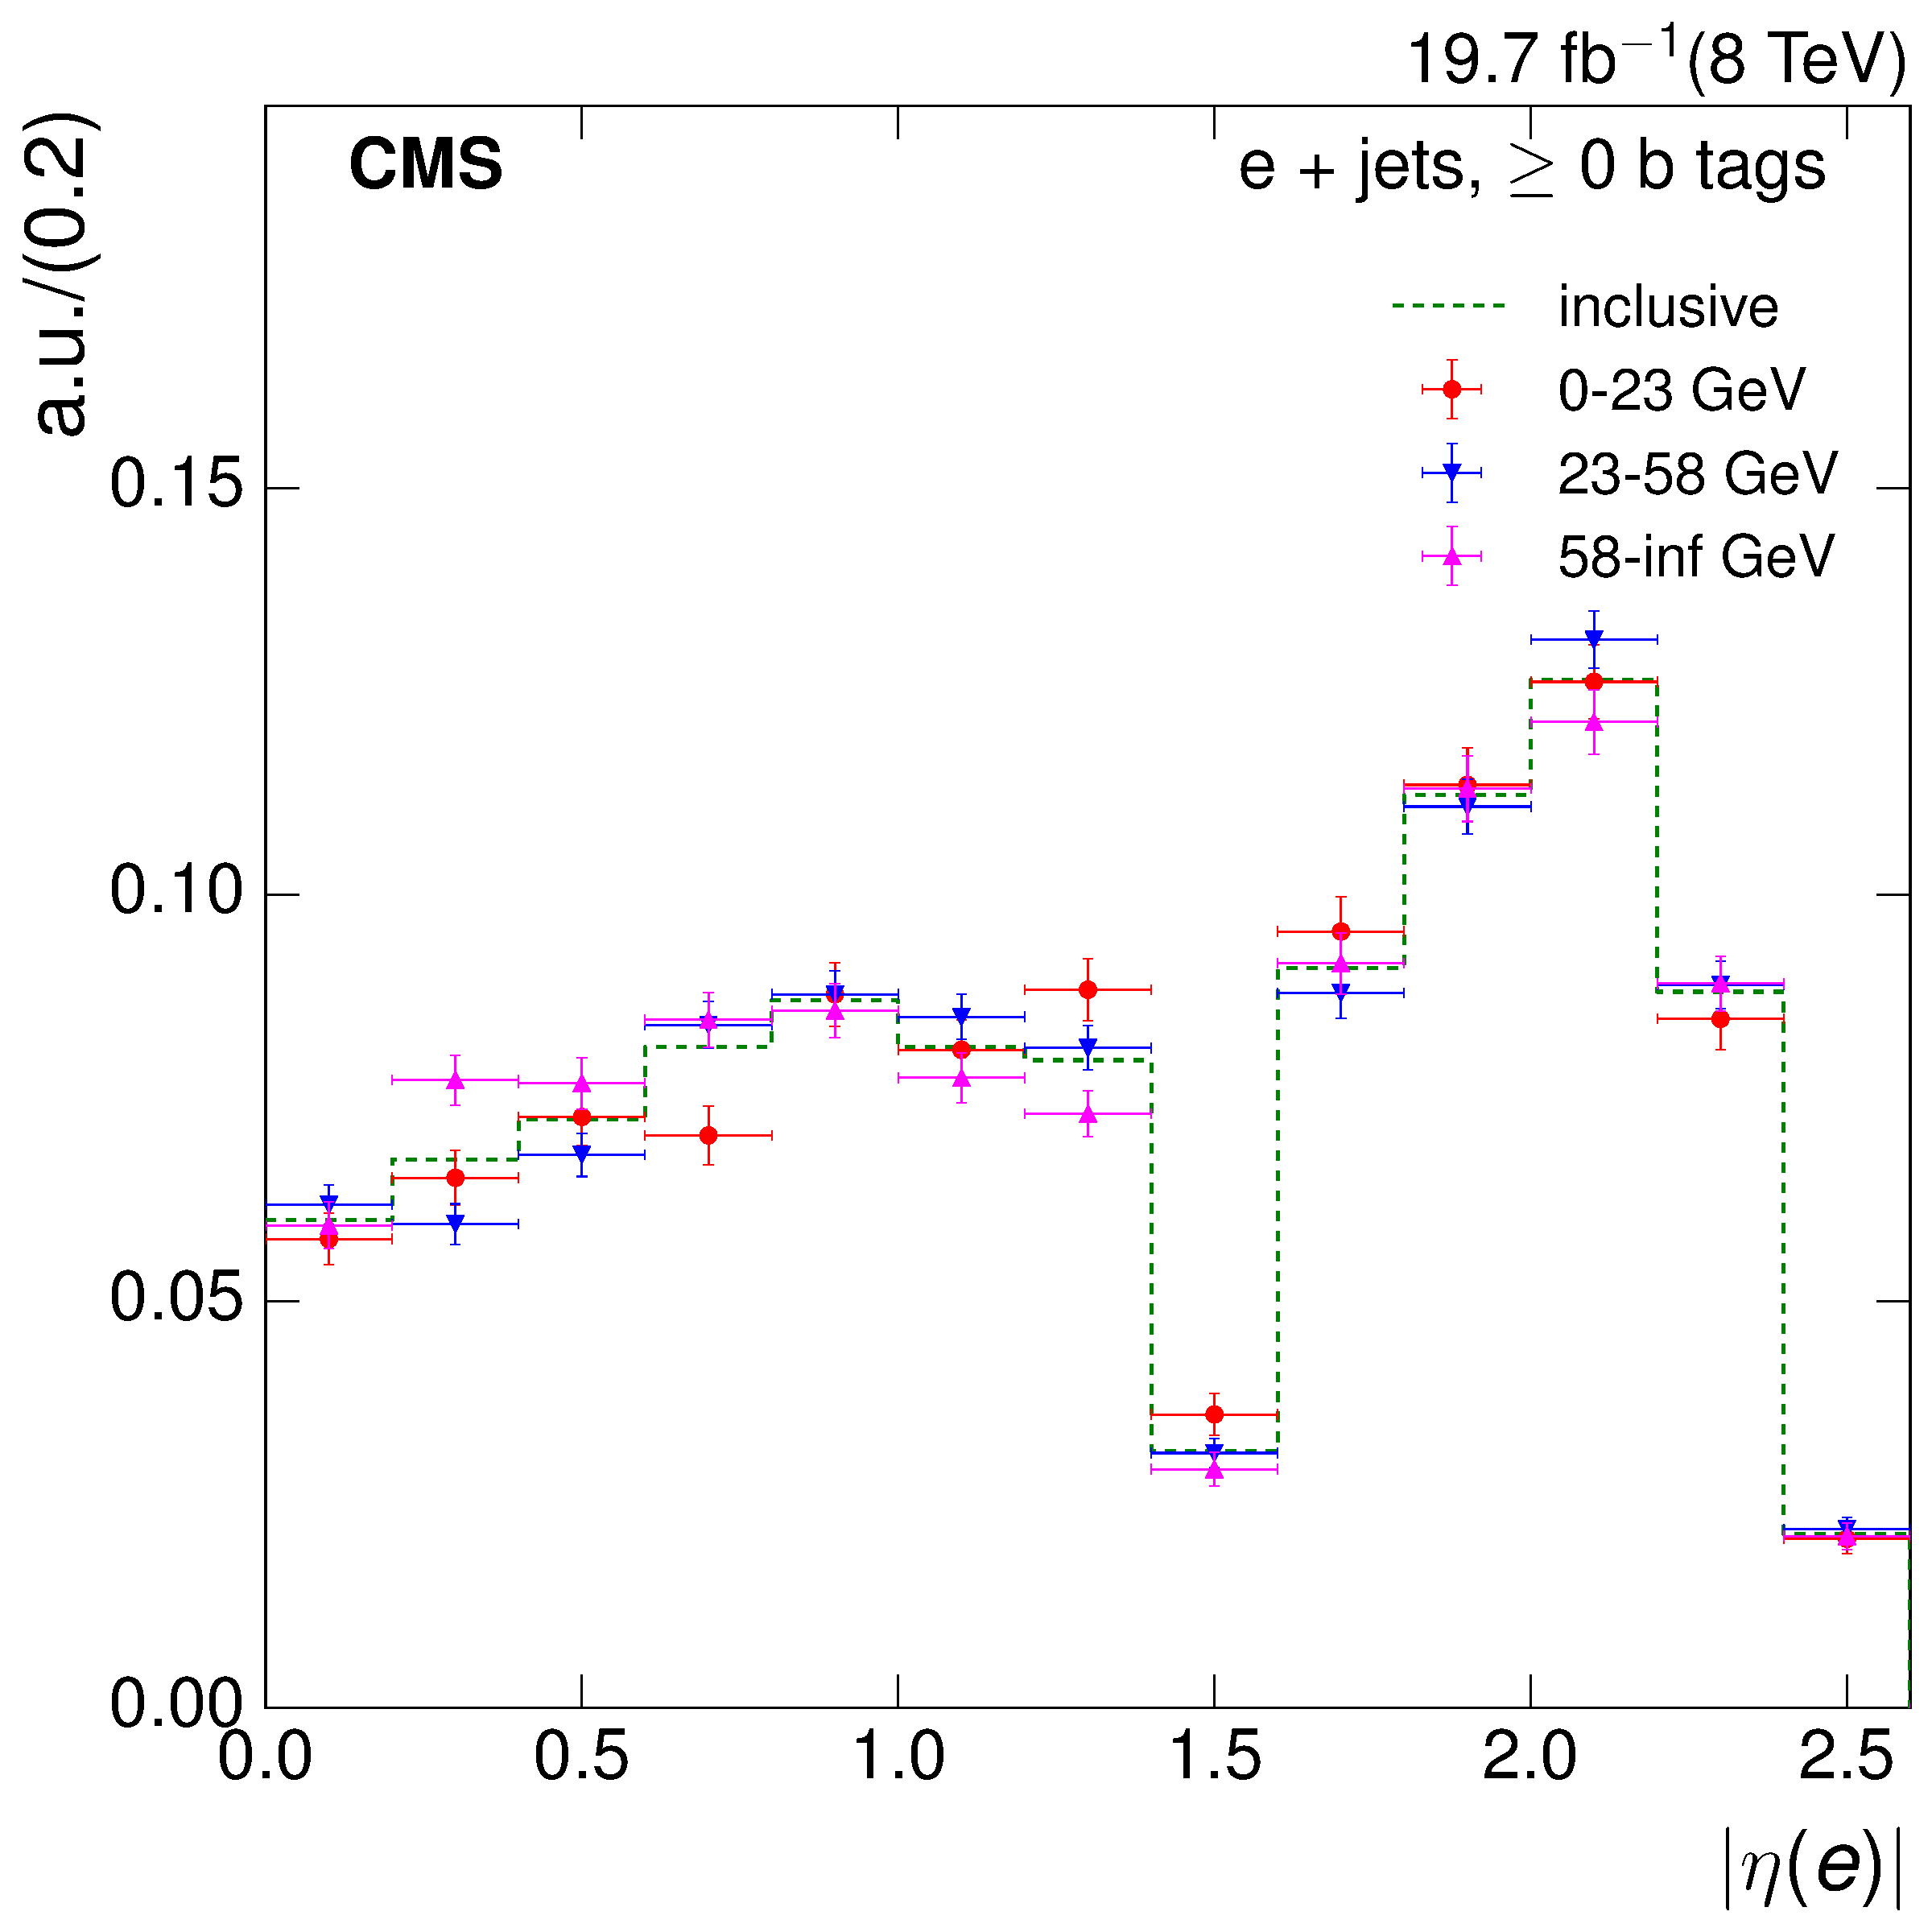
\includegraphics[width=0.48\textwidth]{Chapters/07_08_09_Analysis/Images/8TeV/fit_variables/electron/MT/electron_absolute_eta/qcd/MT_electron_absolute_eta_0orMoreBtag_QCD_template_comparison.pdf}\hfill
% 	 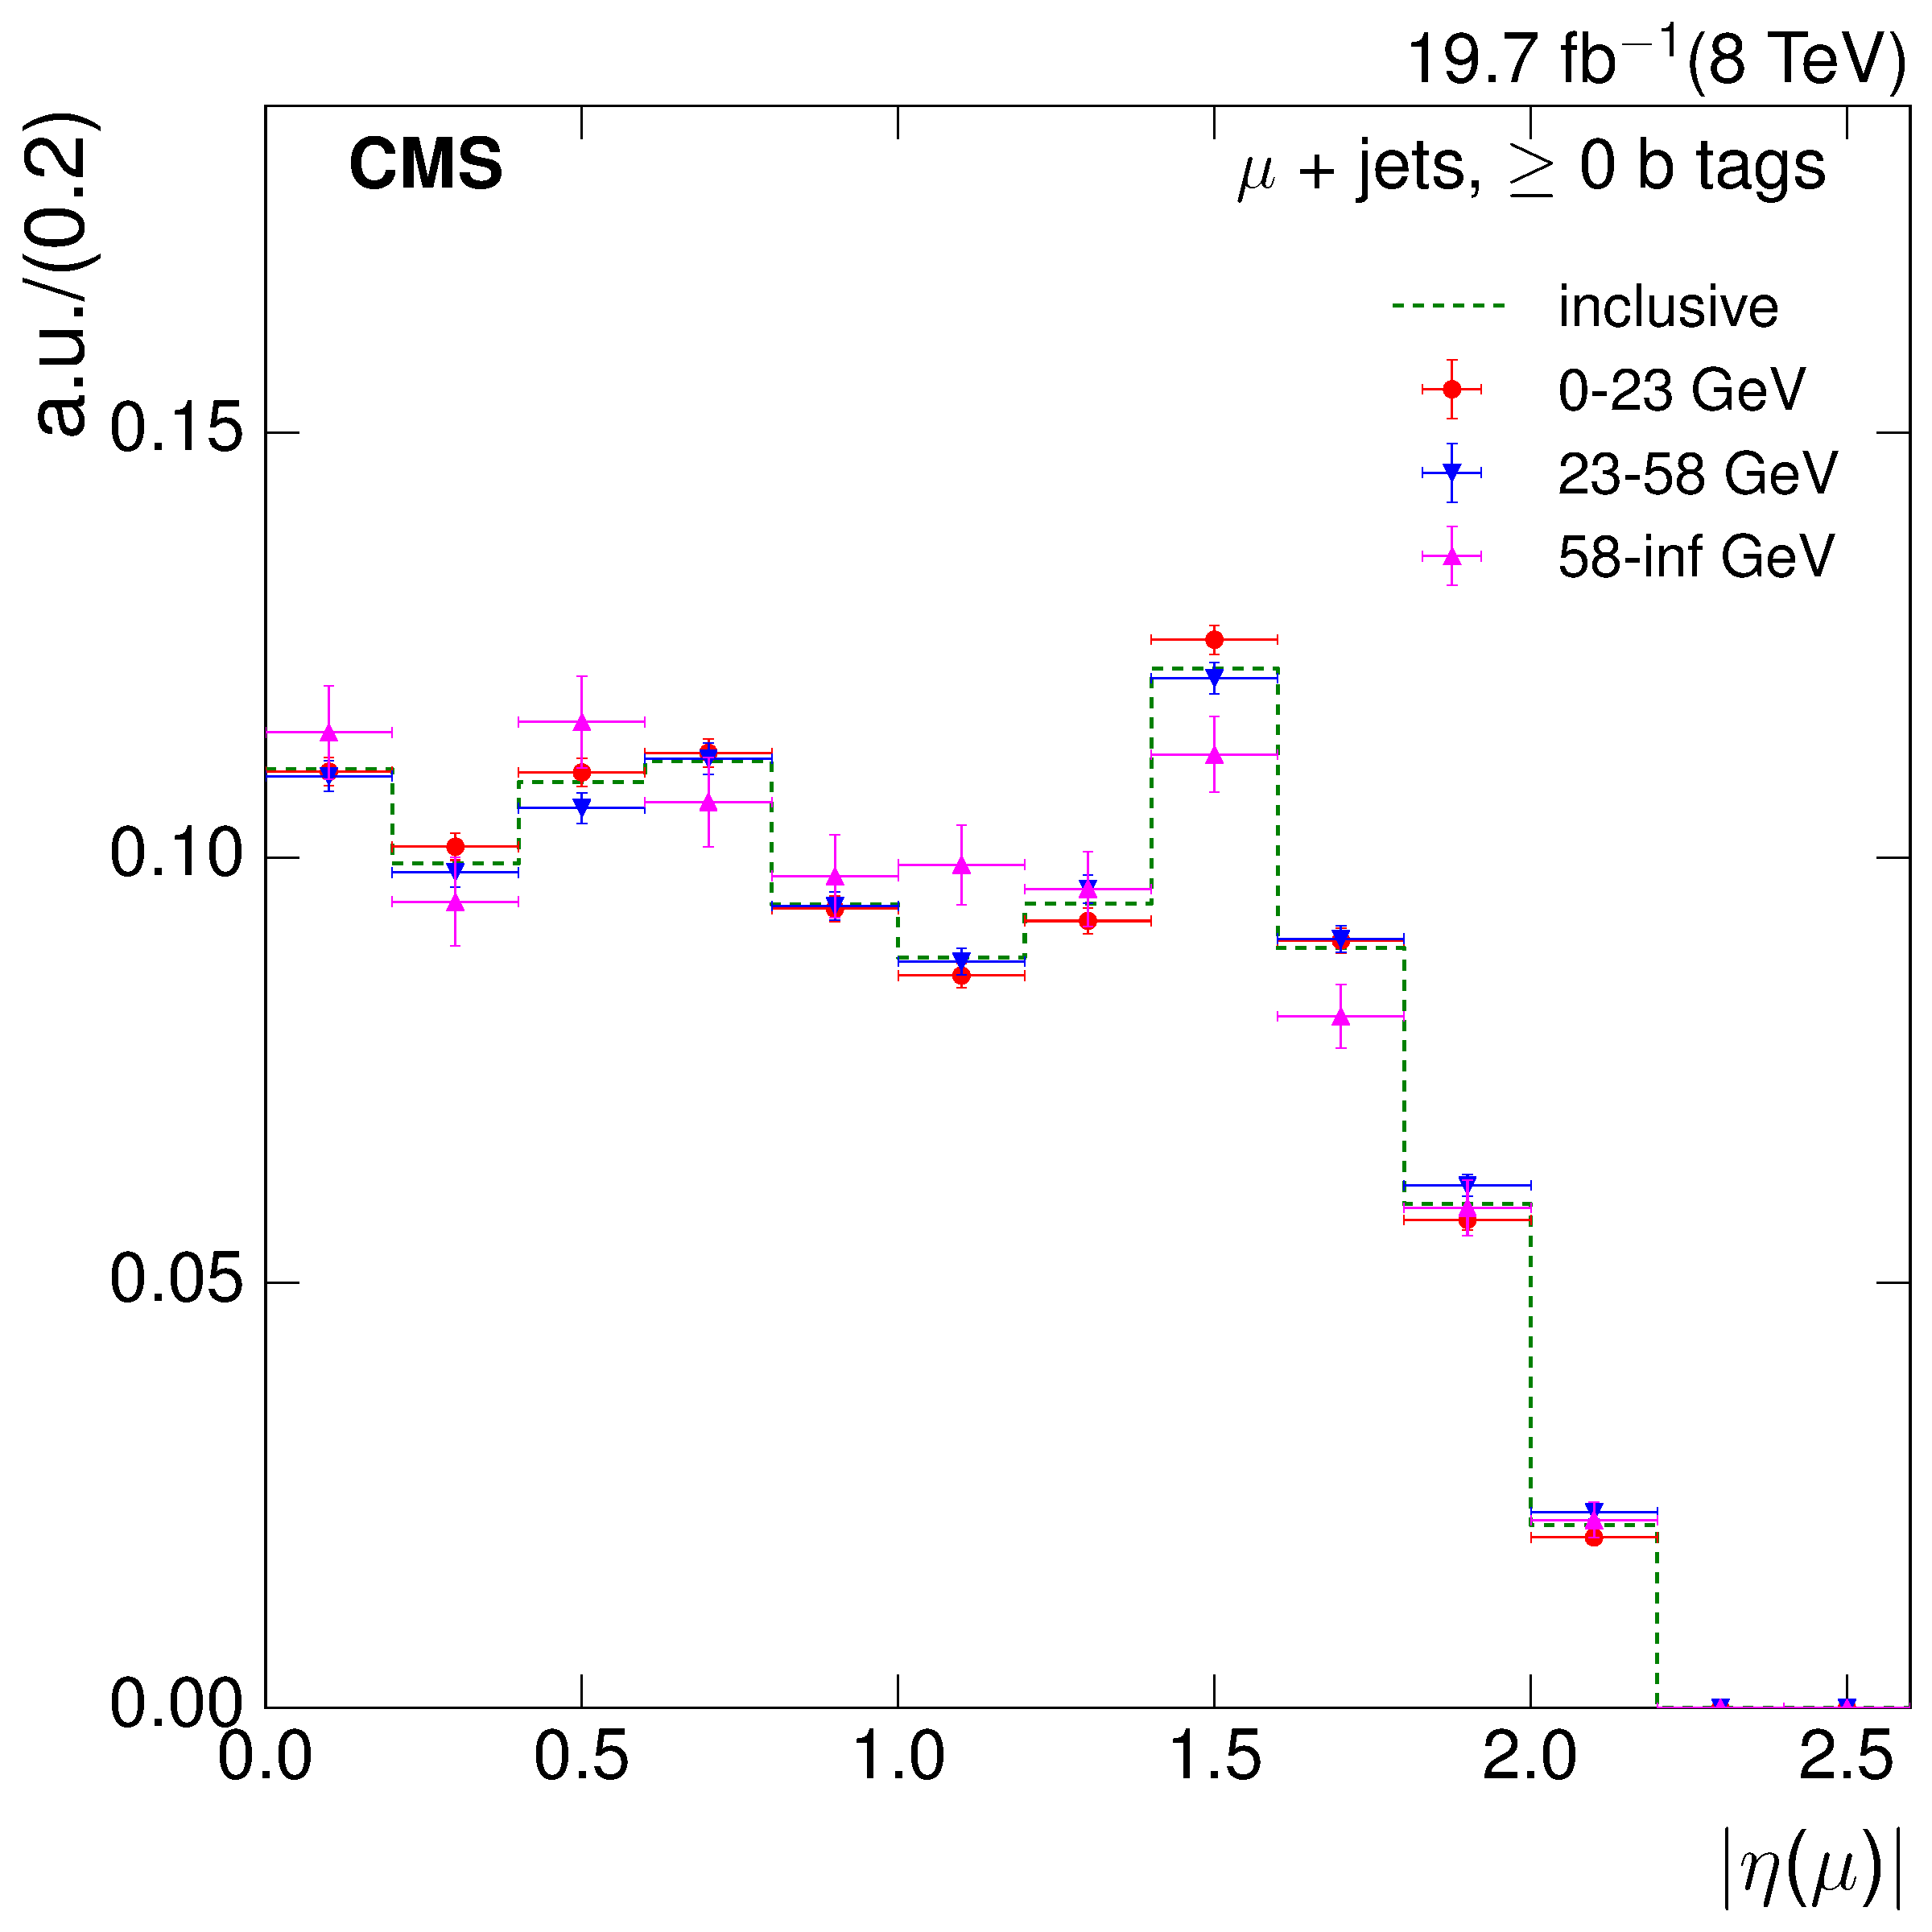
\includegraphics[width=0.48\textwidth]{Chapters/07_08_09_Analysis/Images/8TeV/fit_variables/muon/MT/muon_absolute_eta/qcd/MT_muon_absolute_eta_0orMoreBtag_QCD_template_comparison.pdf}\\
%      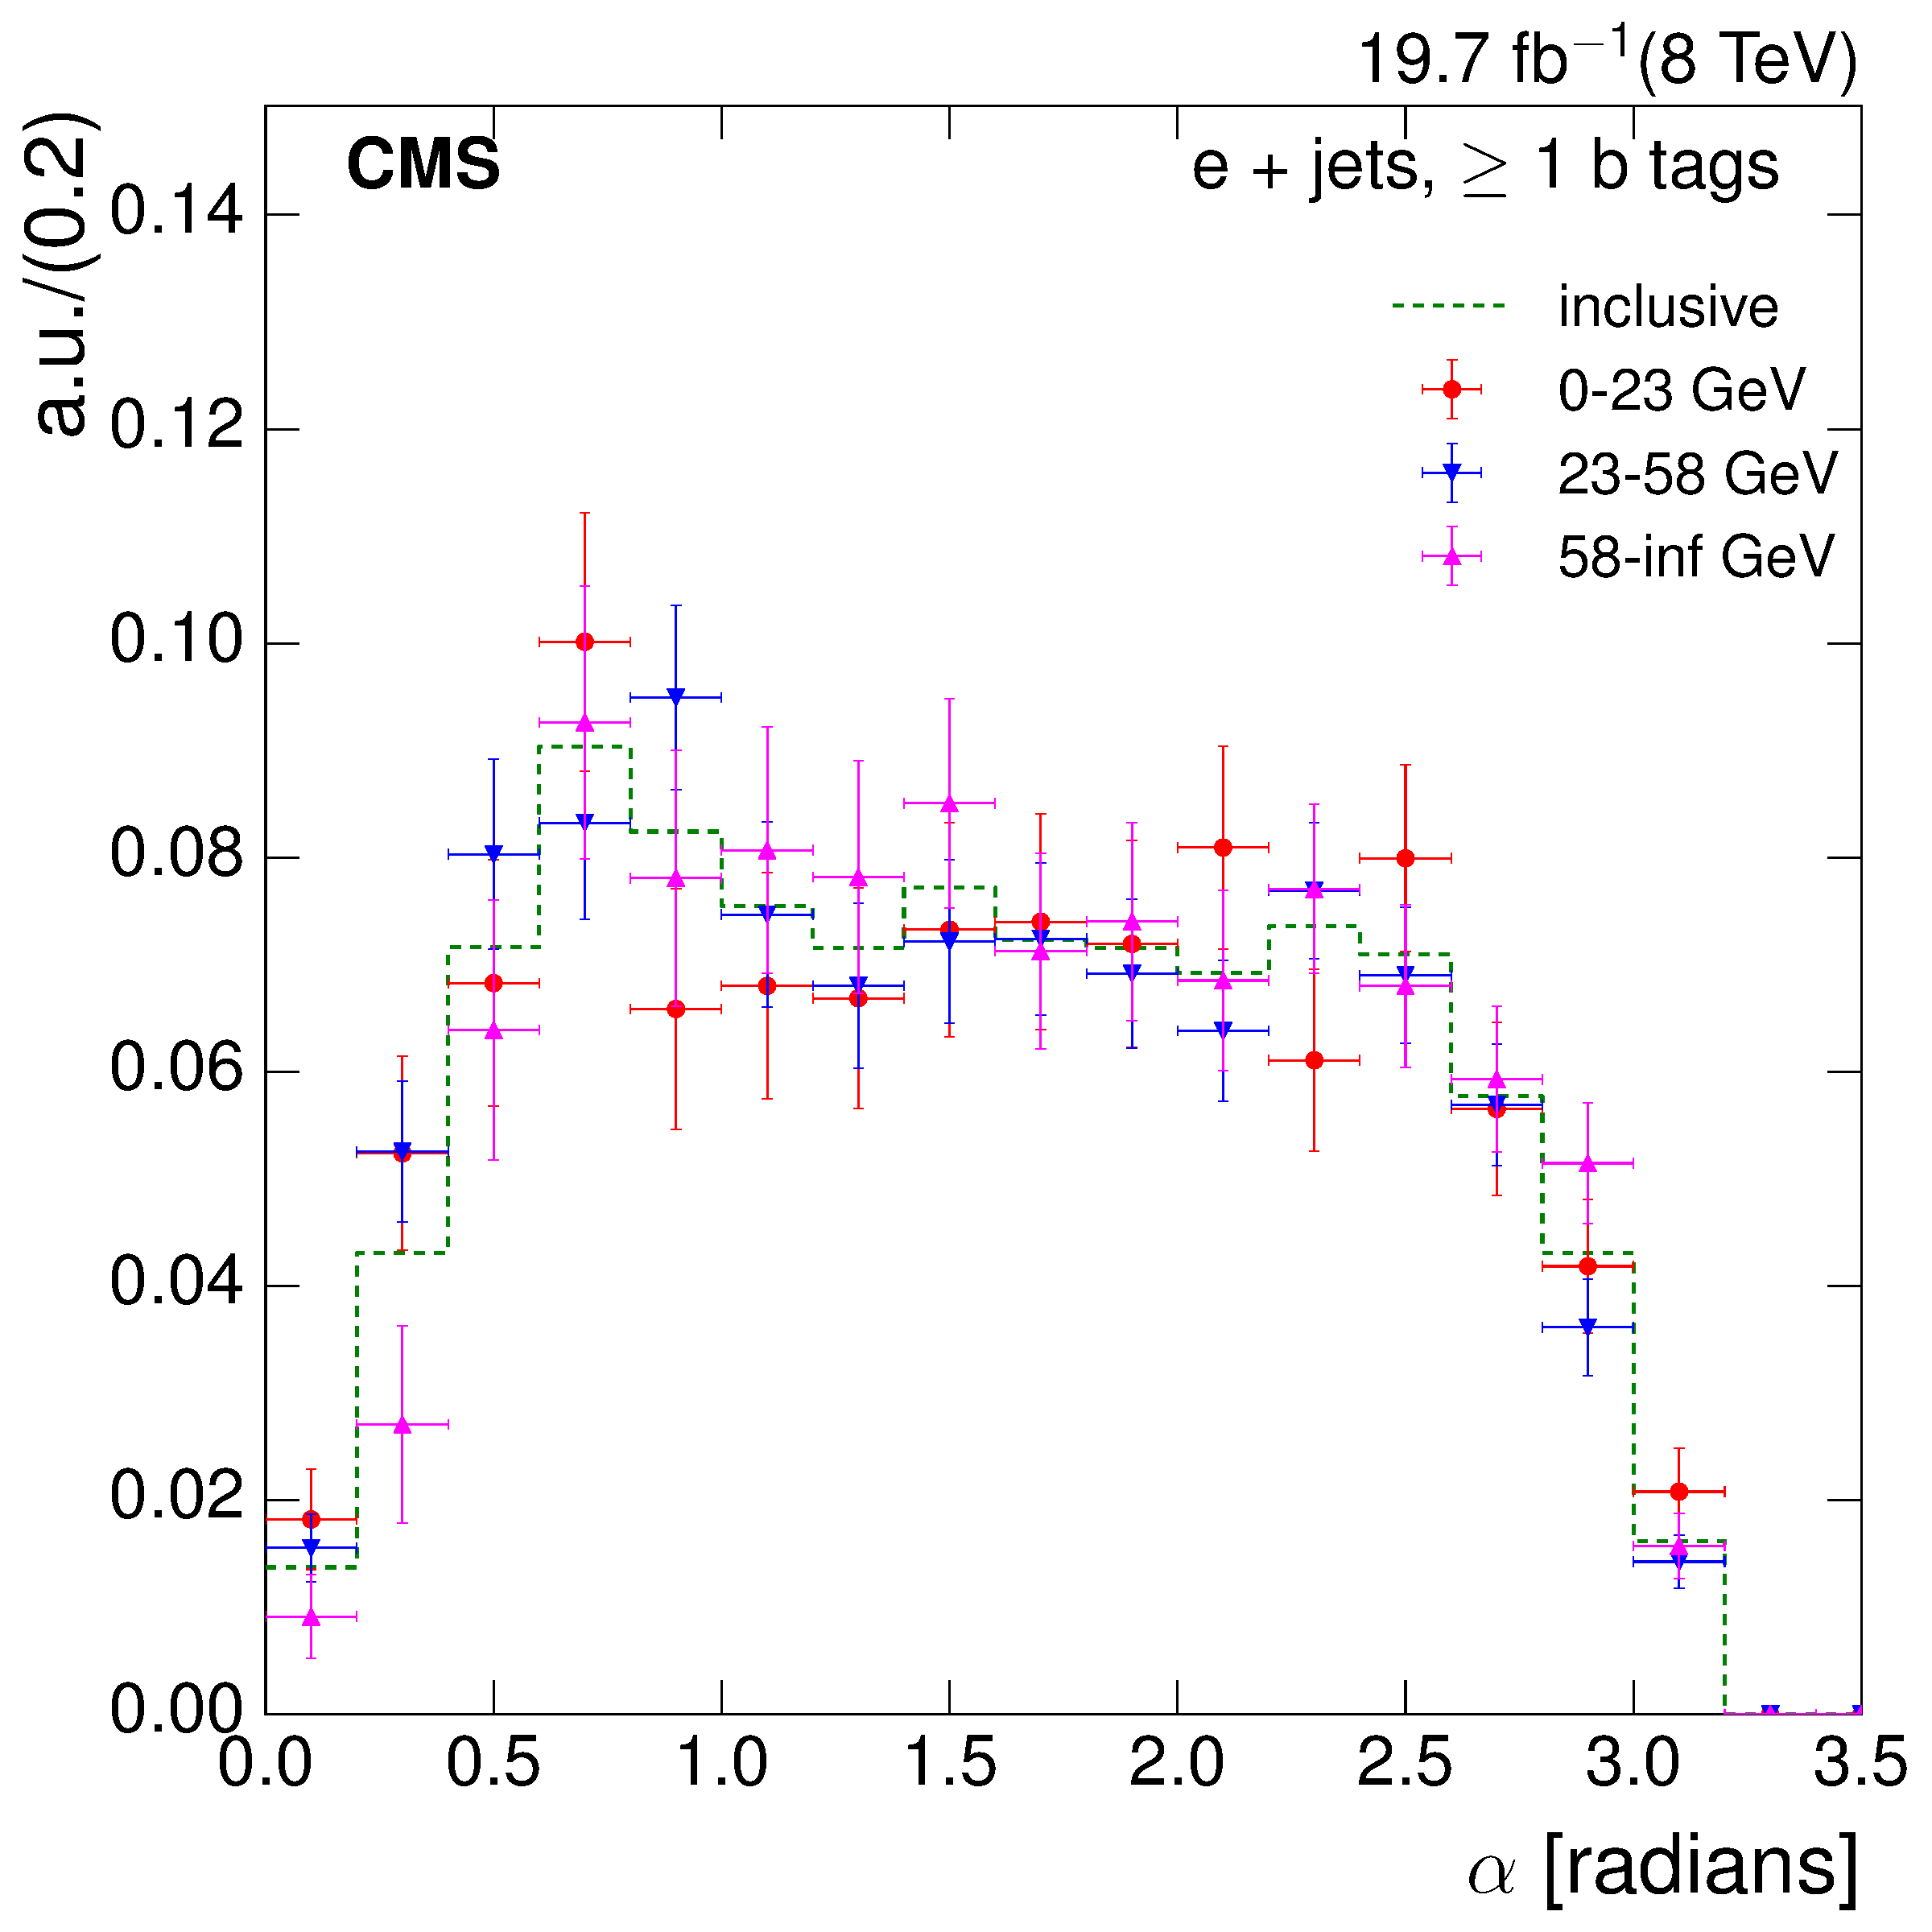
\includegraphics[width=0.48\textwidth]{Chapters/07_08_09_Analysis/Images/8TeV/fit_variables/electron/MT/angle_bl/qcd/MT_angle_bl_1orMoreBtag_QCD_template_comparison.pdf}\hfill
%      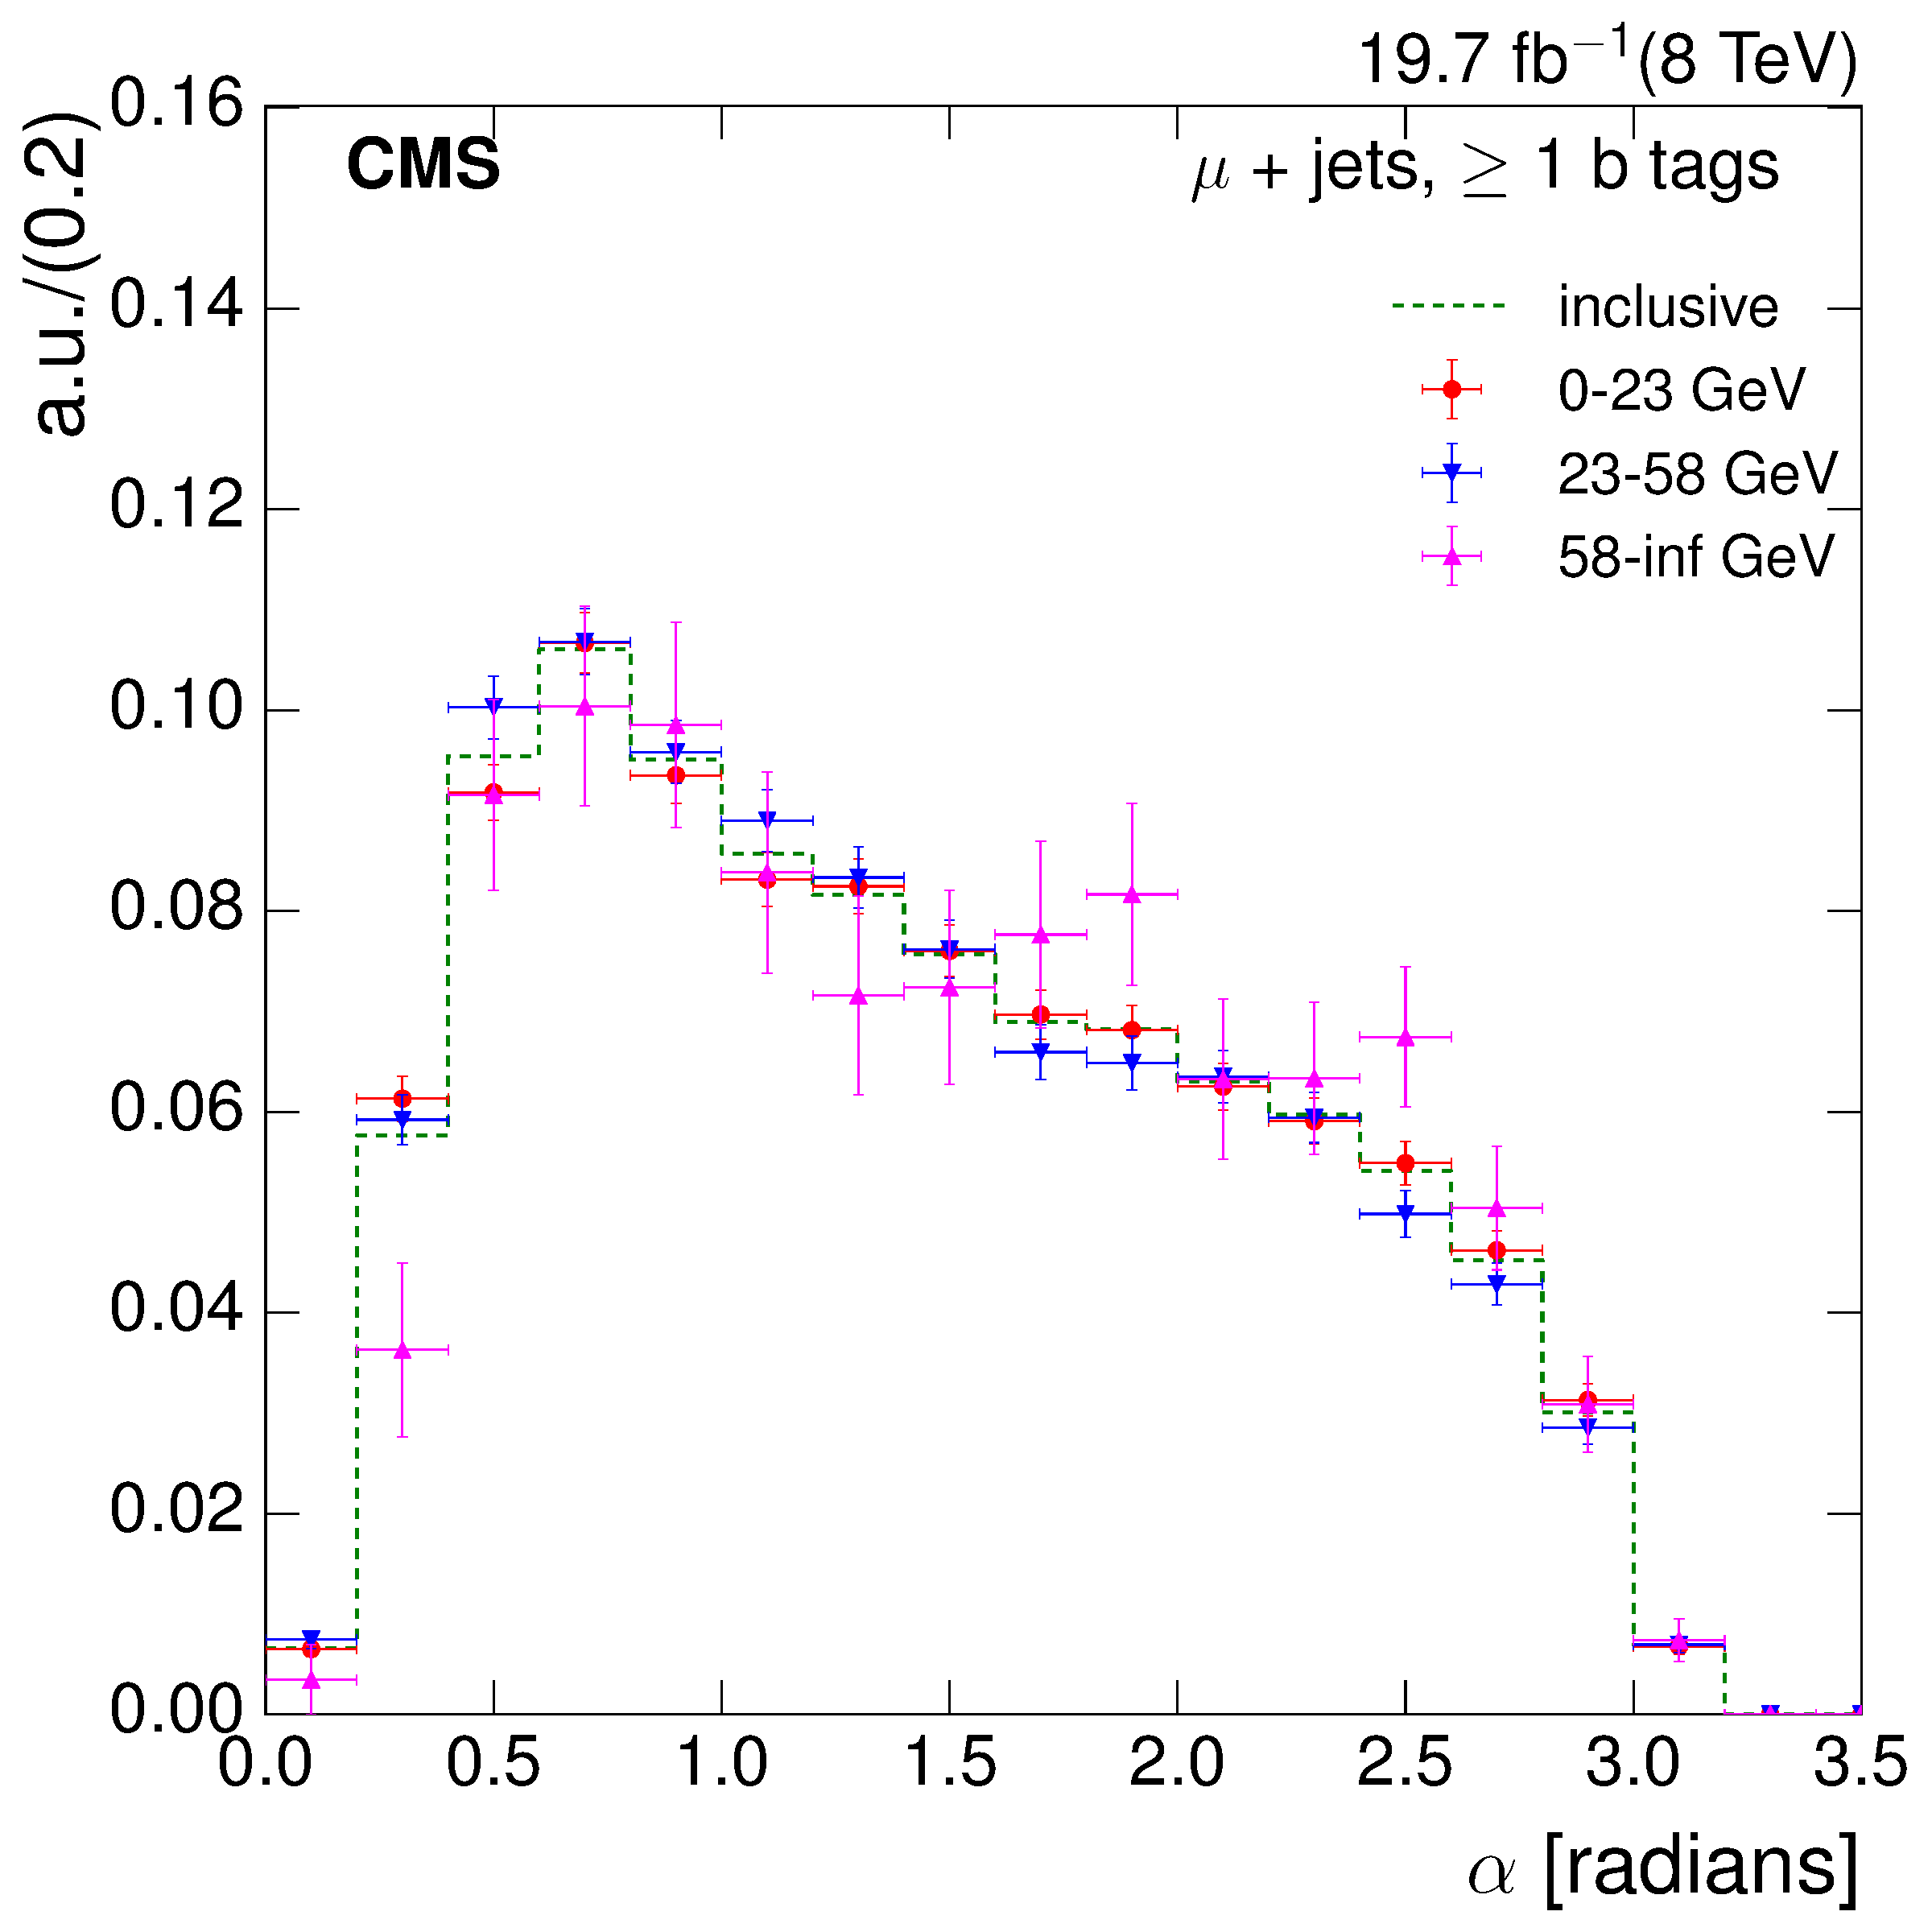
\includegraphics[width=0.48\textwidth]{Chapters/07_08_09_Analysis/Images/8TeV/fit_variables/muon/MT/angle_bl/qcd/MT_angle_bl_1orMoreBtag_QCD_template_comparison.pdf}\\
%      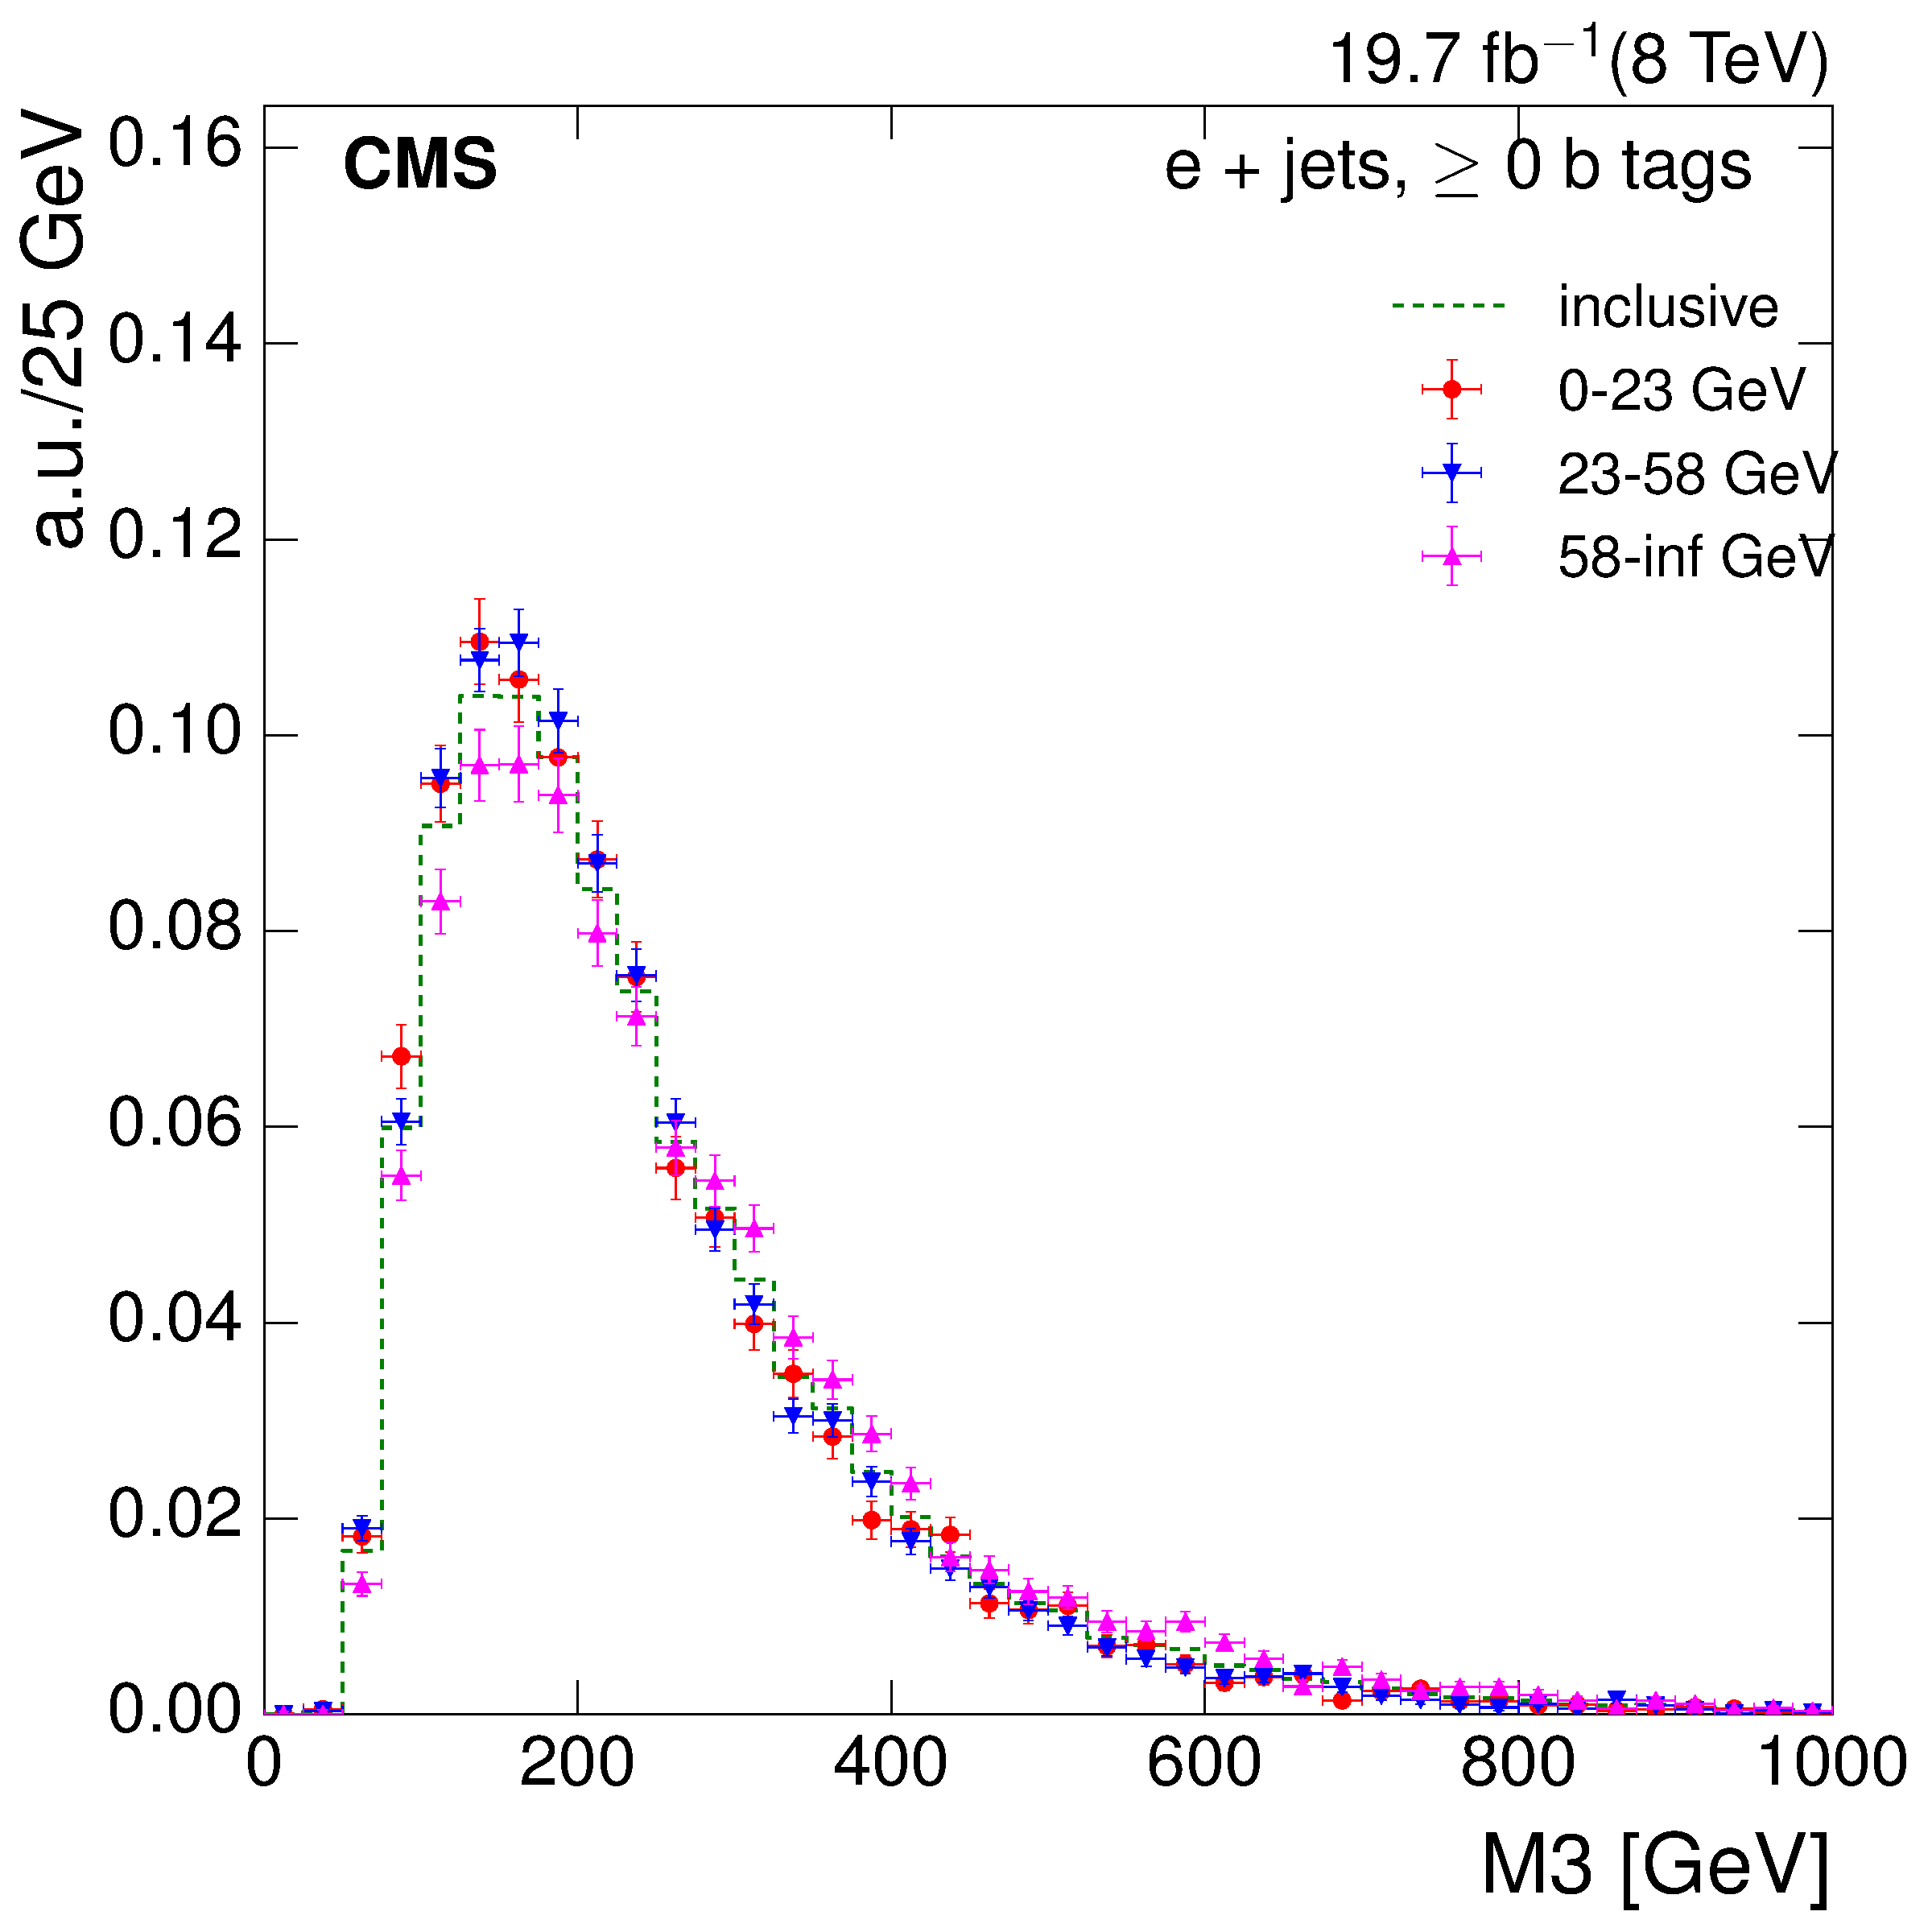
\includegraphics[width=0.48\textwidth]{Chapters/07_08_09_Analysis/Images/8TeV/fit_variables/electron/MT/M3/qcd/MT_M3_0orMoreBtag_QCD_template_comparison.pdf}\hfill
%      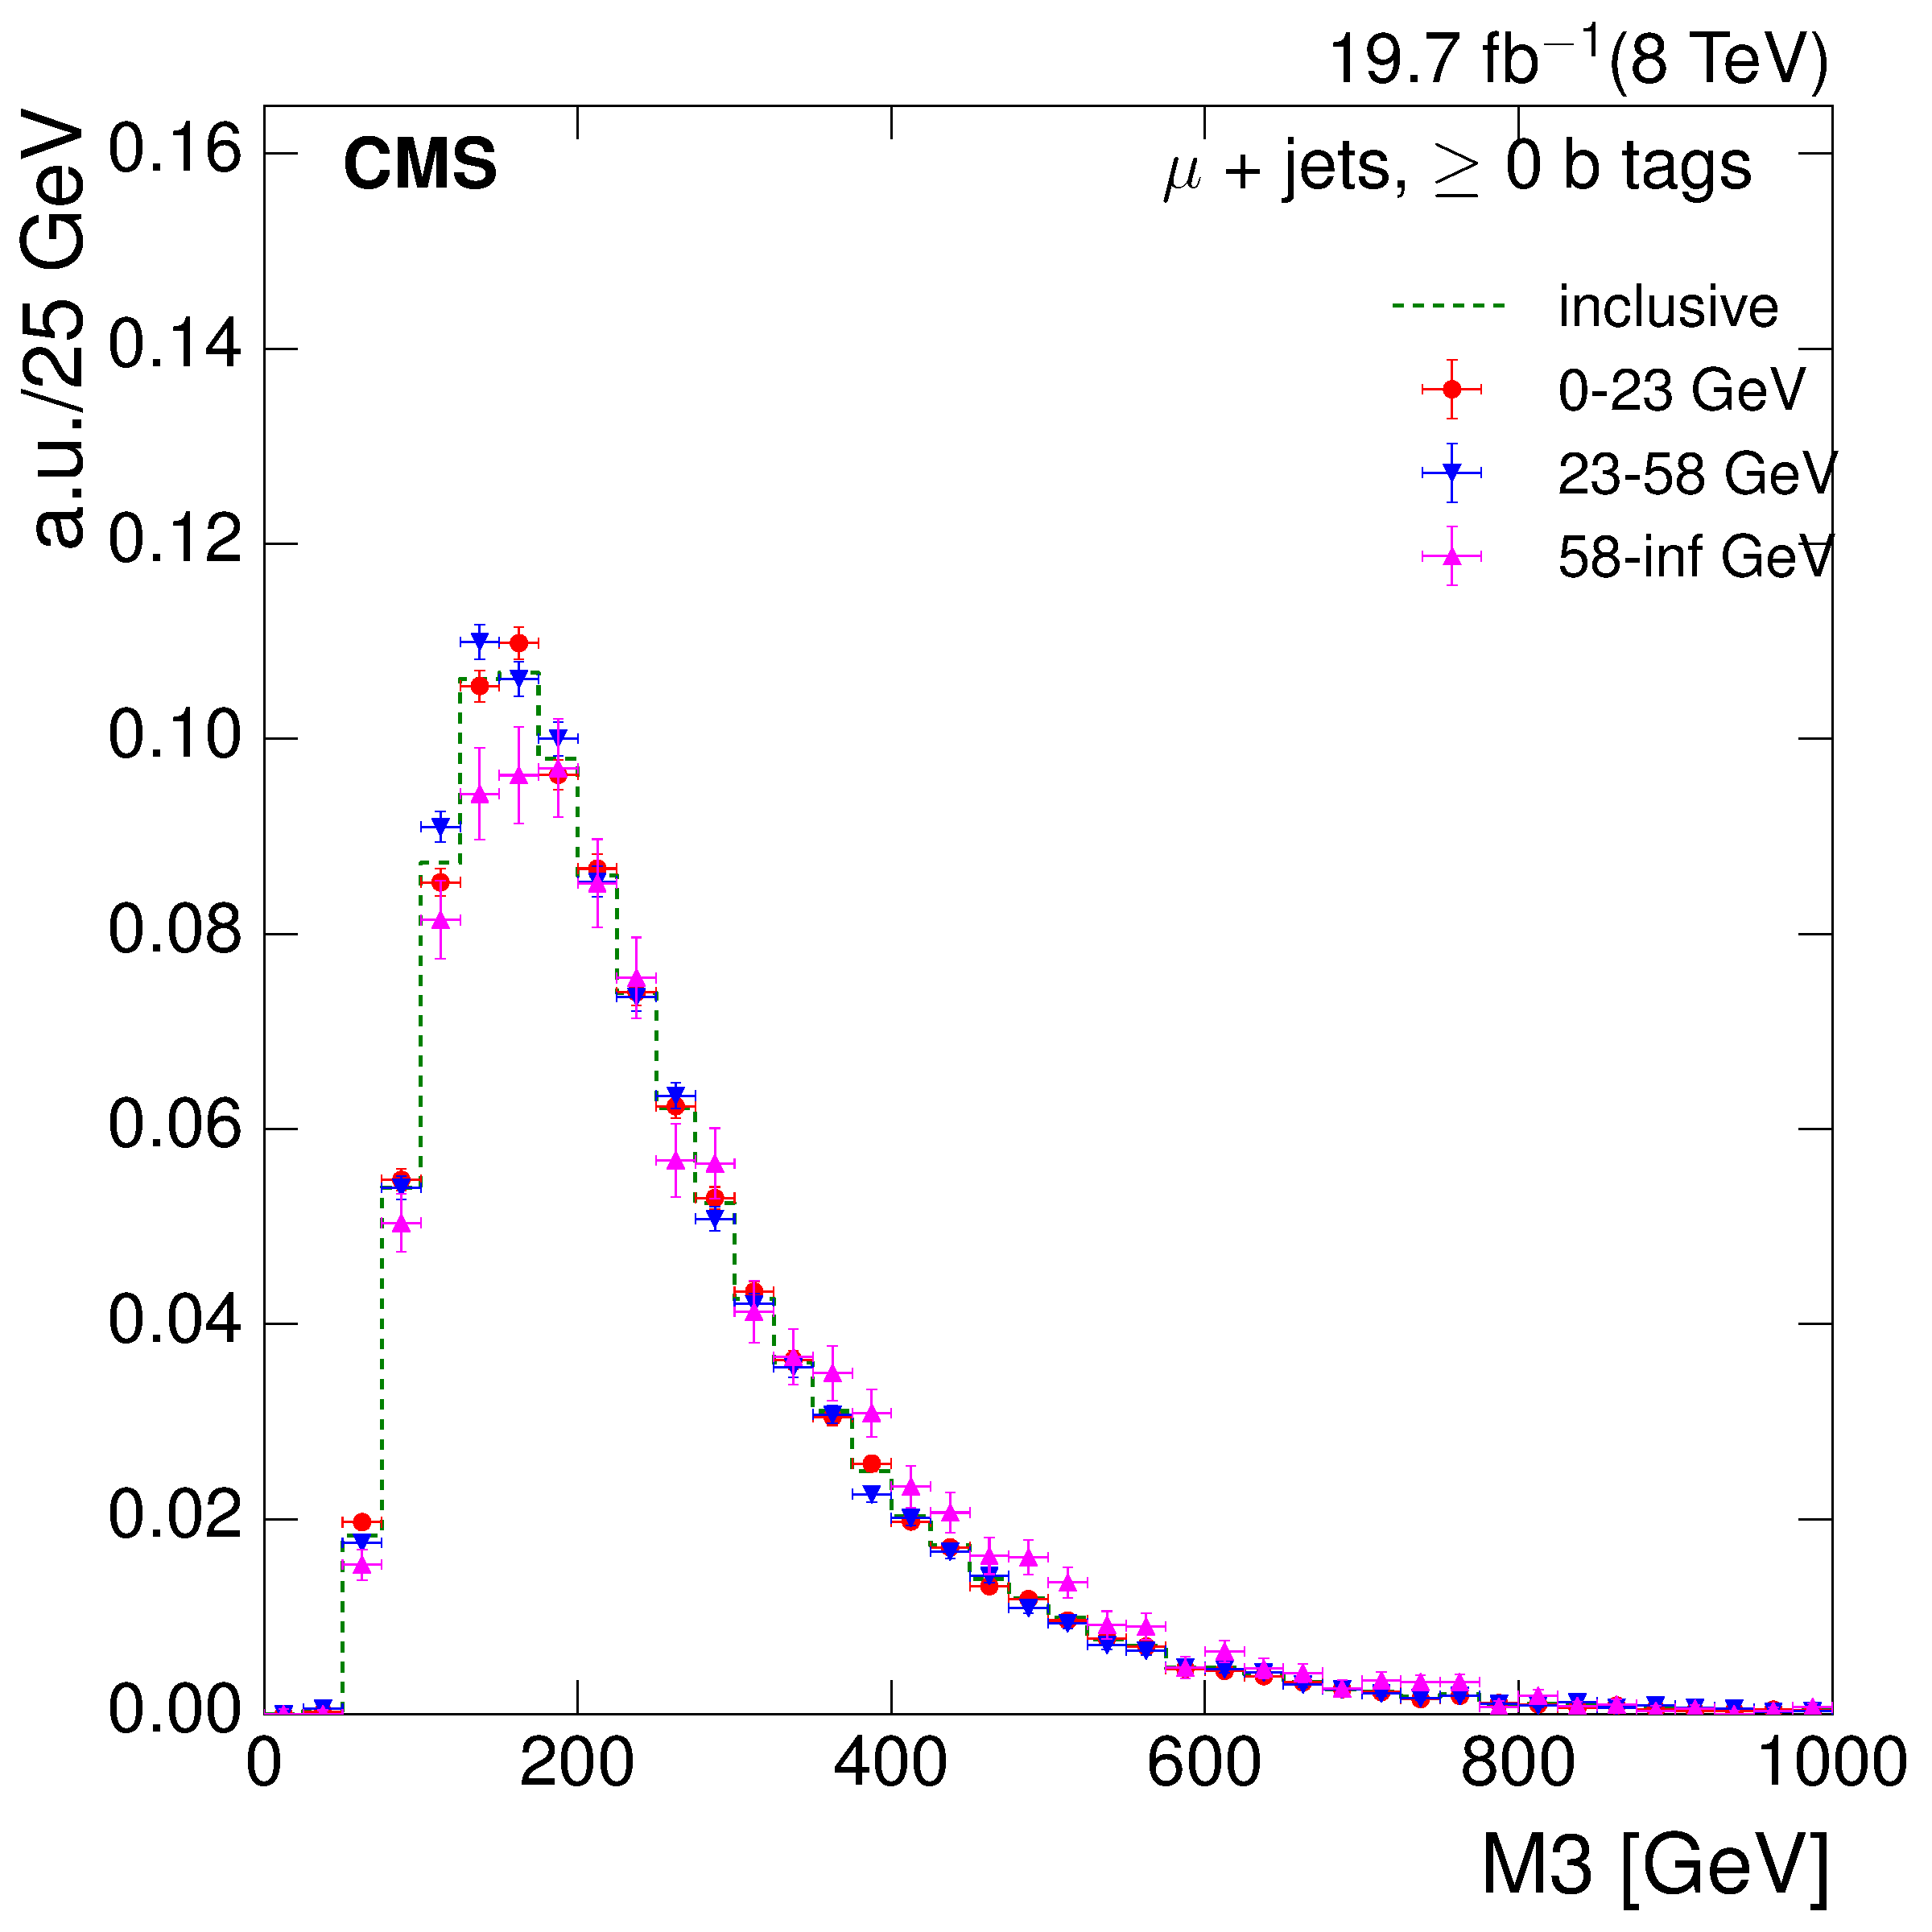
\includegraphics[width=0.48\textwidth]{Chapters/07_08_09_Analysis/Images/8TeV/fit_variables/muon/MT/M3/qcd/MT_M3_0orMoreBtag_QCD_template_comparison.pdf}\\
% 	 \caption[Normalised distributions of the QCD templates for the three fit variables in \mt bins
% 	 at $\sqrt{s}=8\TeV$.]{Normalised distributions of the QCD templates for the three fit variables lepton
% 	 \abseta (upper), $\alpha$ (middle) and M3 (lower) inclusive across all \mt bins and for the lowest three \mt
% 	 bins at $\sqrt{s}=8\TeV$ in the electron+jets channel (left) and in the muon+jets channel (right).}
%      \label{fig:MT_fit_variable_qcd_comparisons_8TeV}
% \end{figure}
% 
% \begin{figure}[hbtp]
%     \centering
%      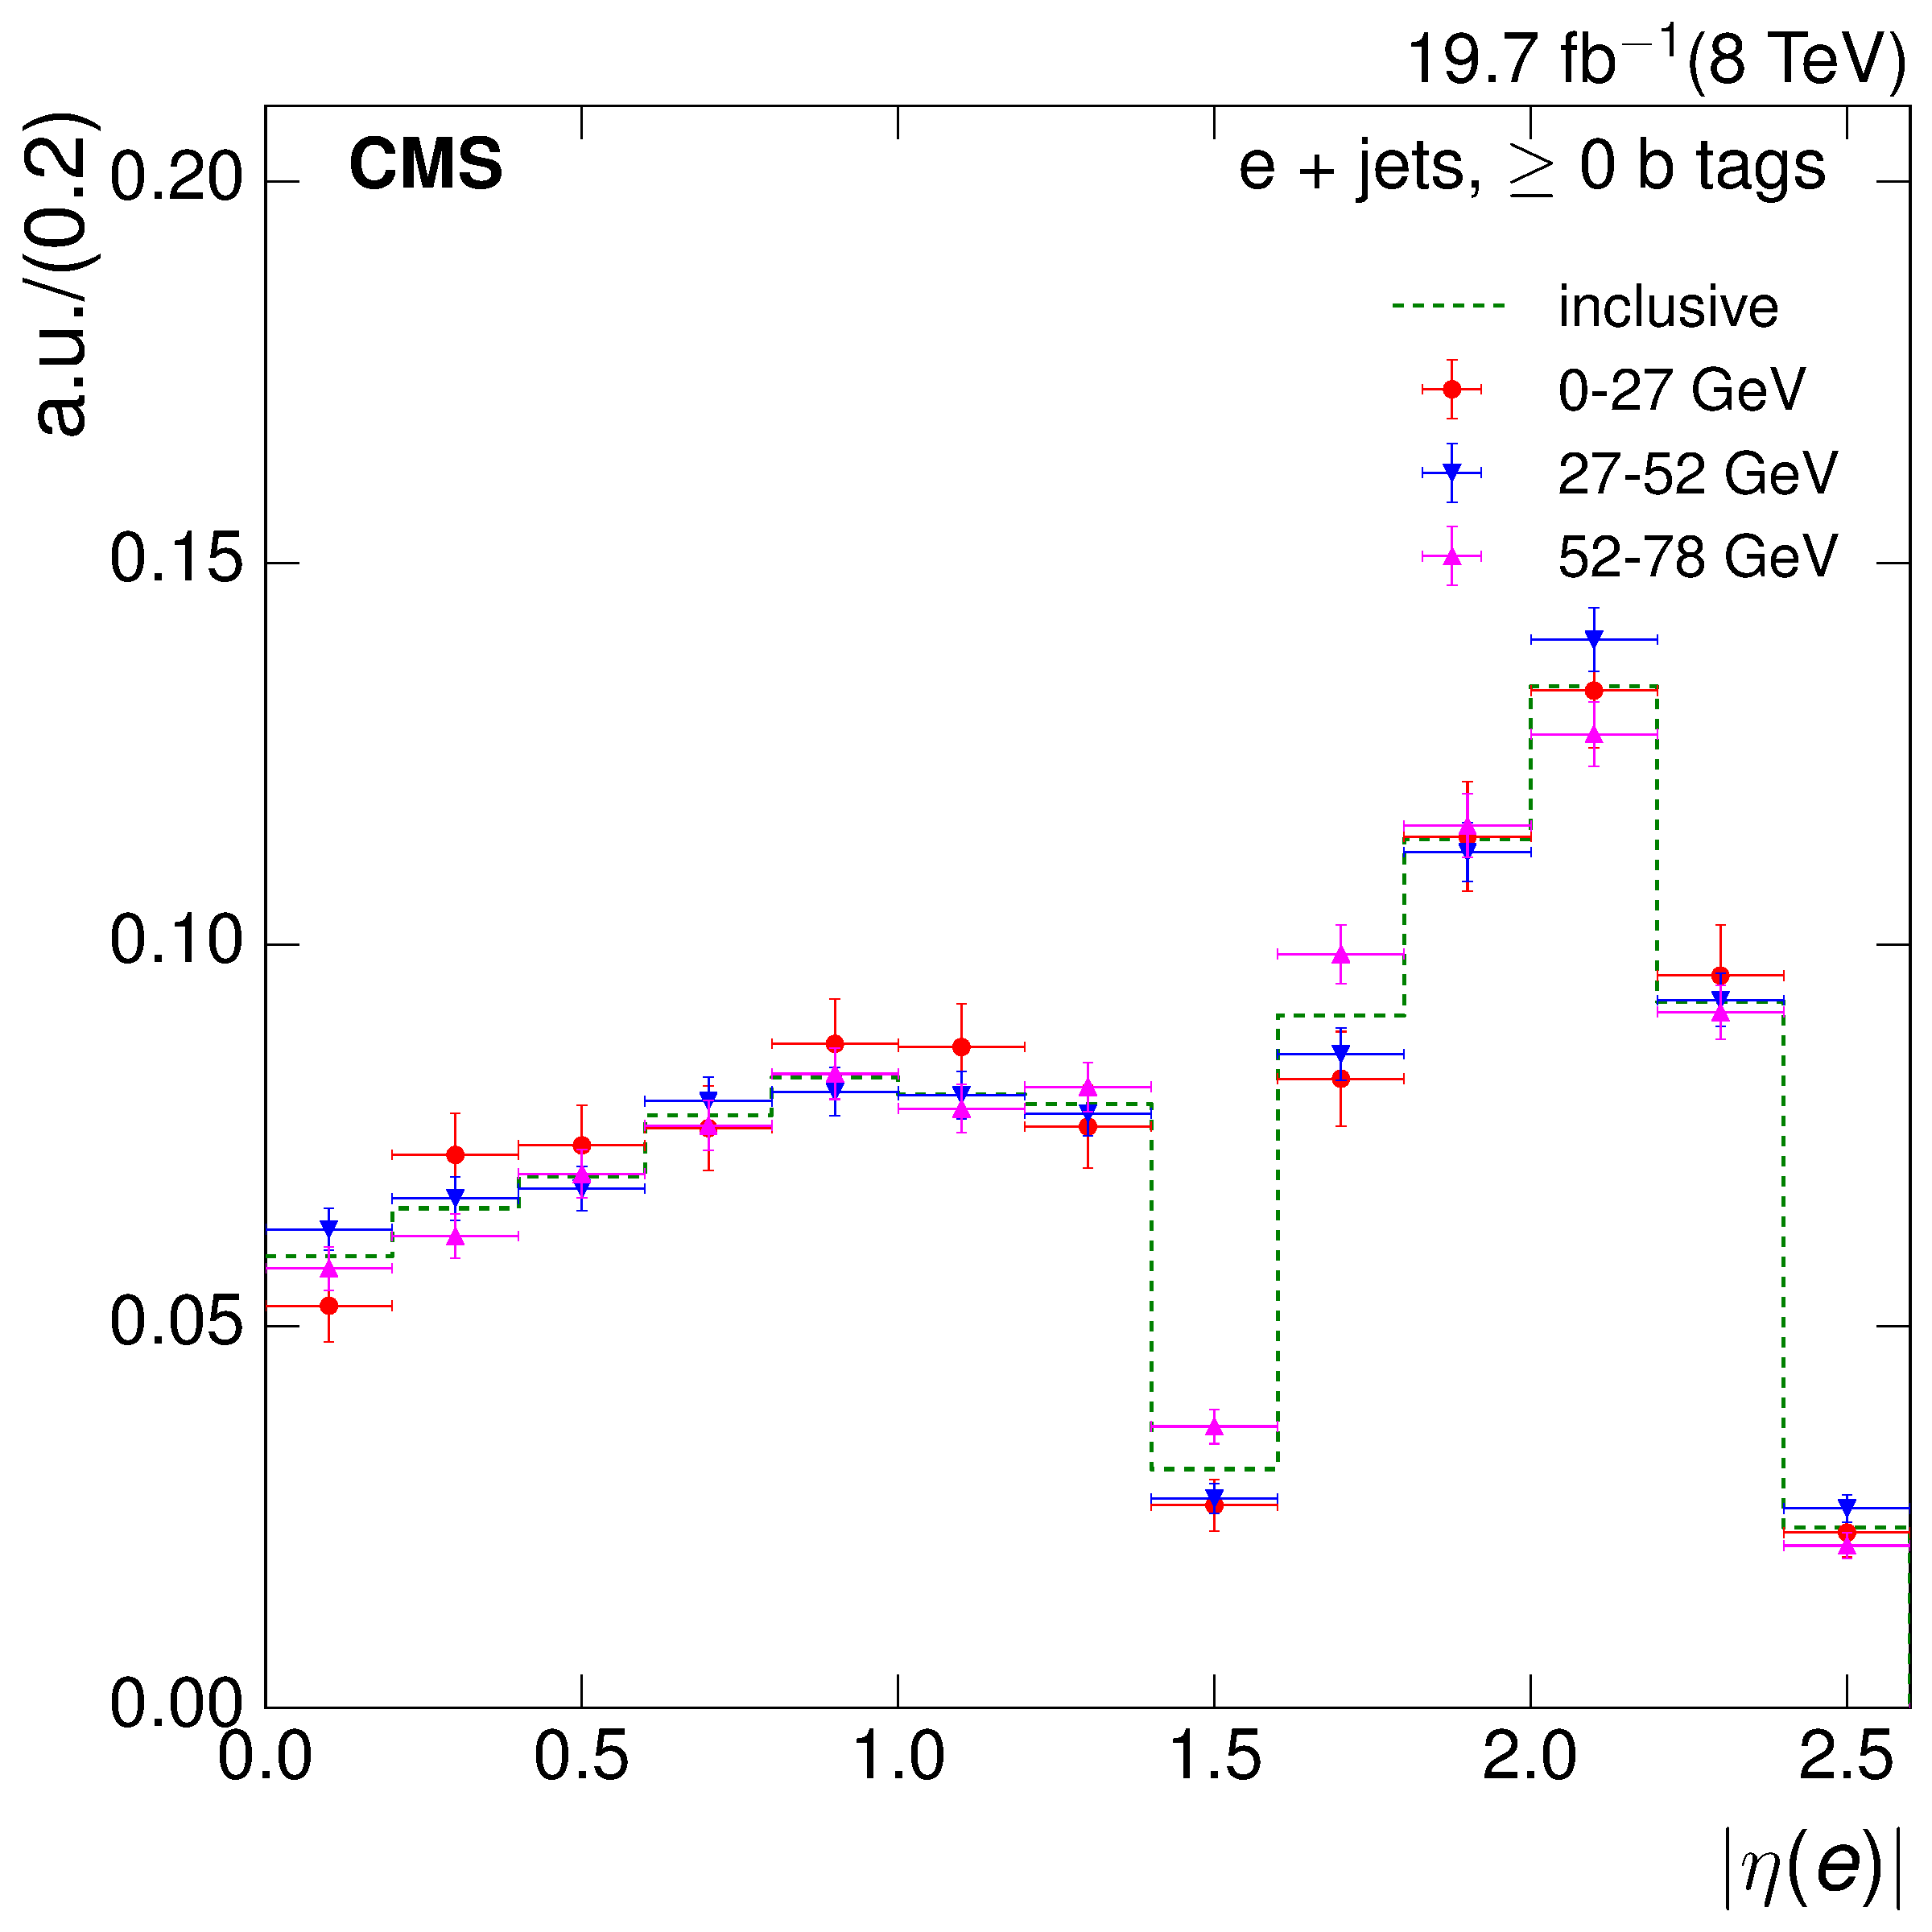
\includegraphics[width=0.48\textwidth]{Chapters/07_08_09_Analysis/Images/8TeV/fit_variables/electron/WPT/electron_absolute_eta/qcd/WPT_electron_absolute_eta_0orMoreBtag_QCD_template_comparison.pdf}\hfill
%      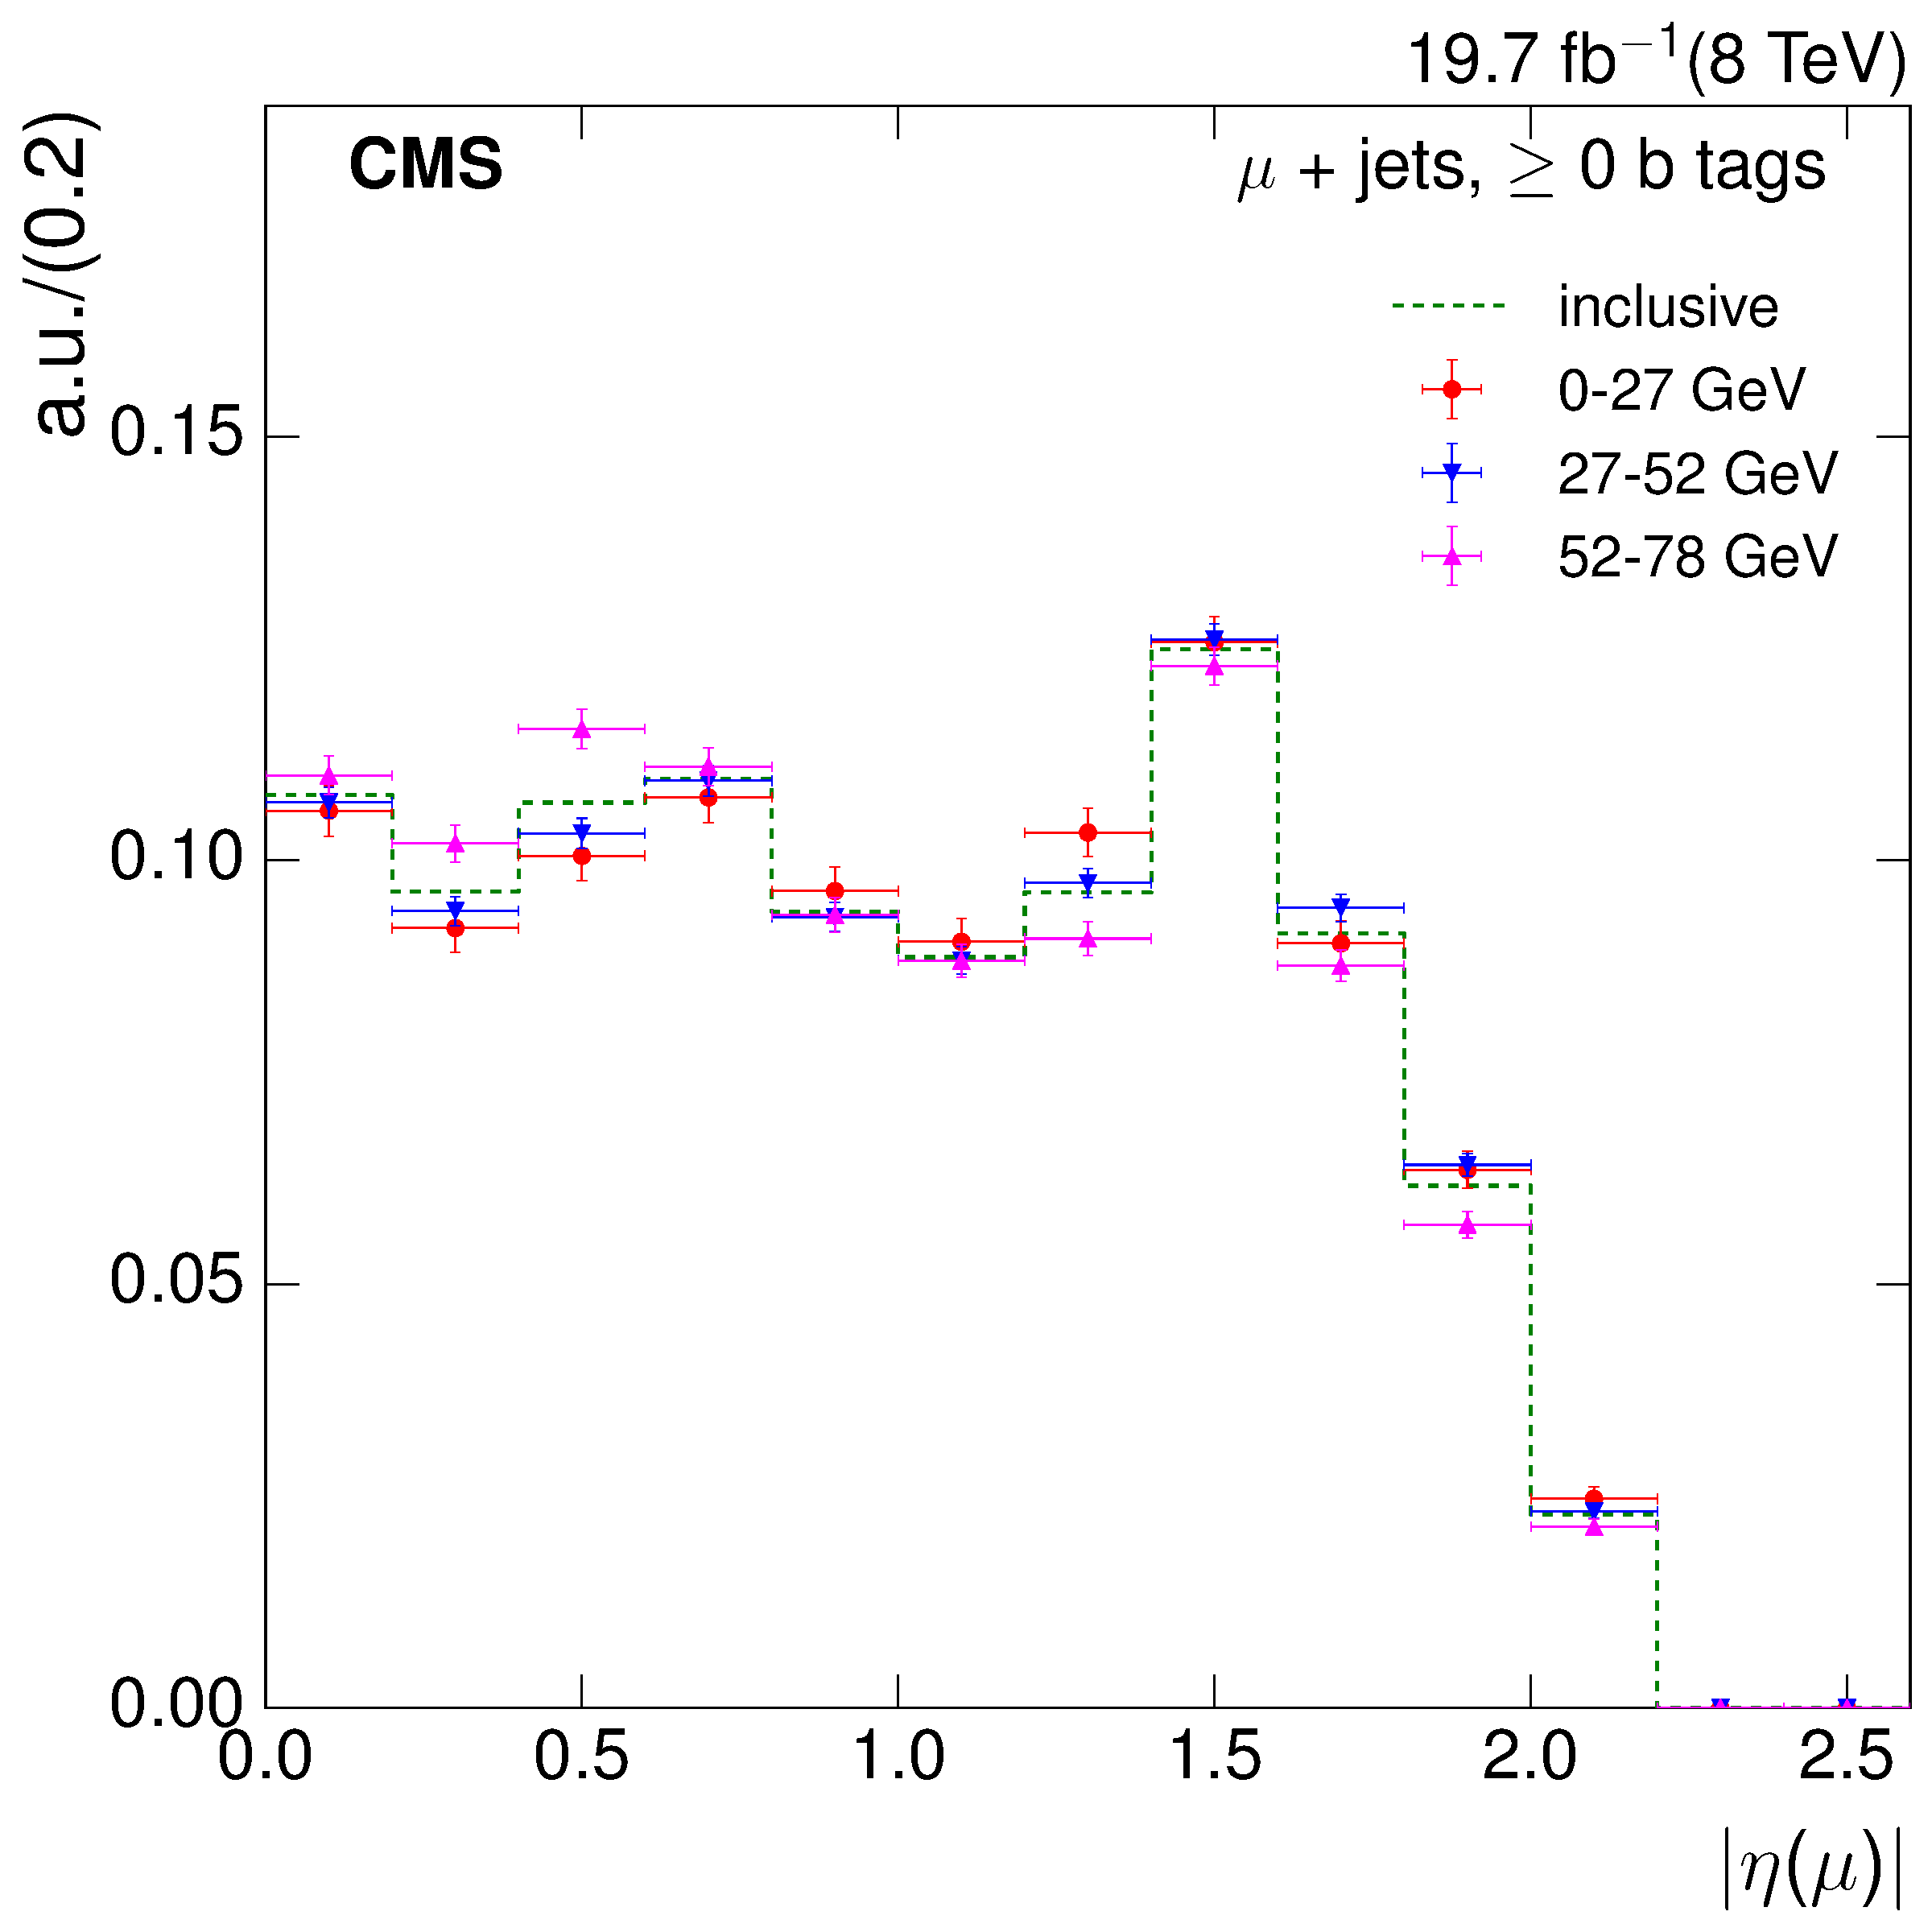
\includegraphics[width=0.48\textwidth]{Chapters/07_08_09_Analysis/Images/8TeV/fit_variables/muon/WPT/muon_absolute_eta/qcd/WPT_muon_absolute_eta_0orMoreBtag_QCD_template_comparison.pdf}\\
%      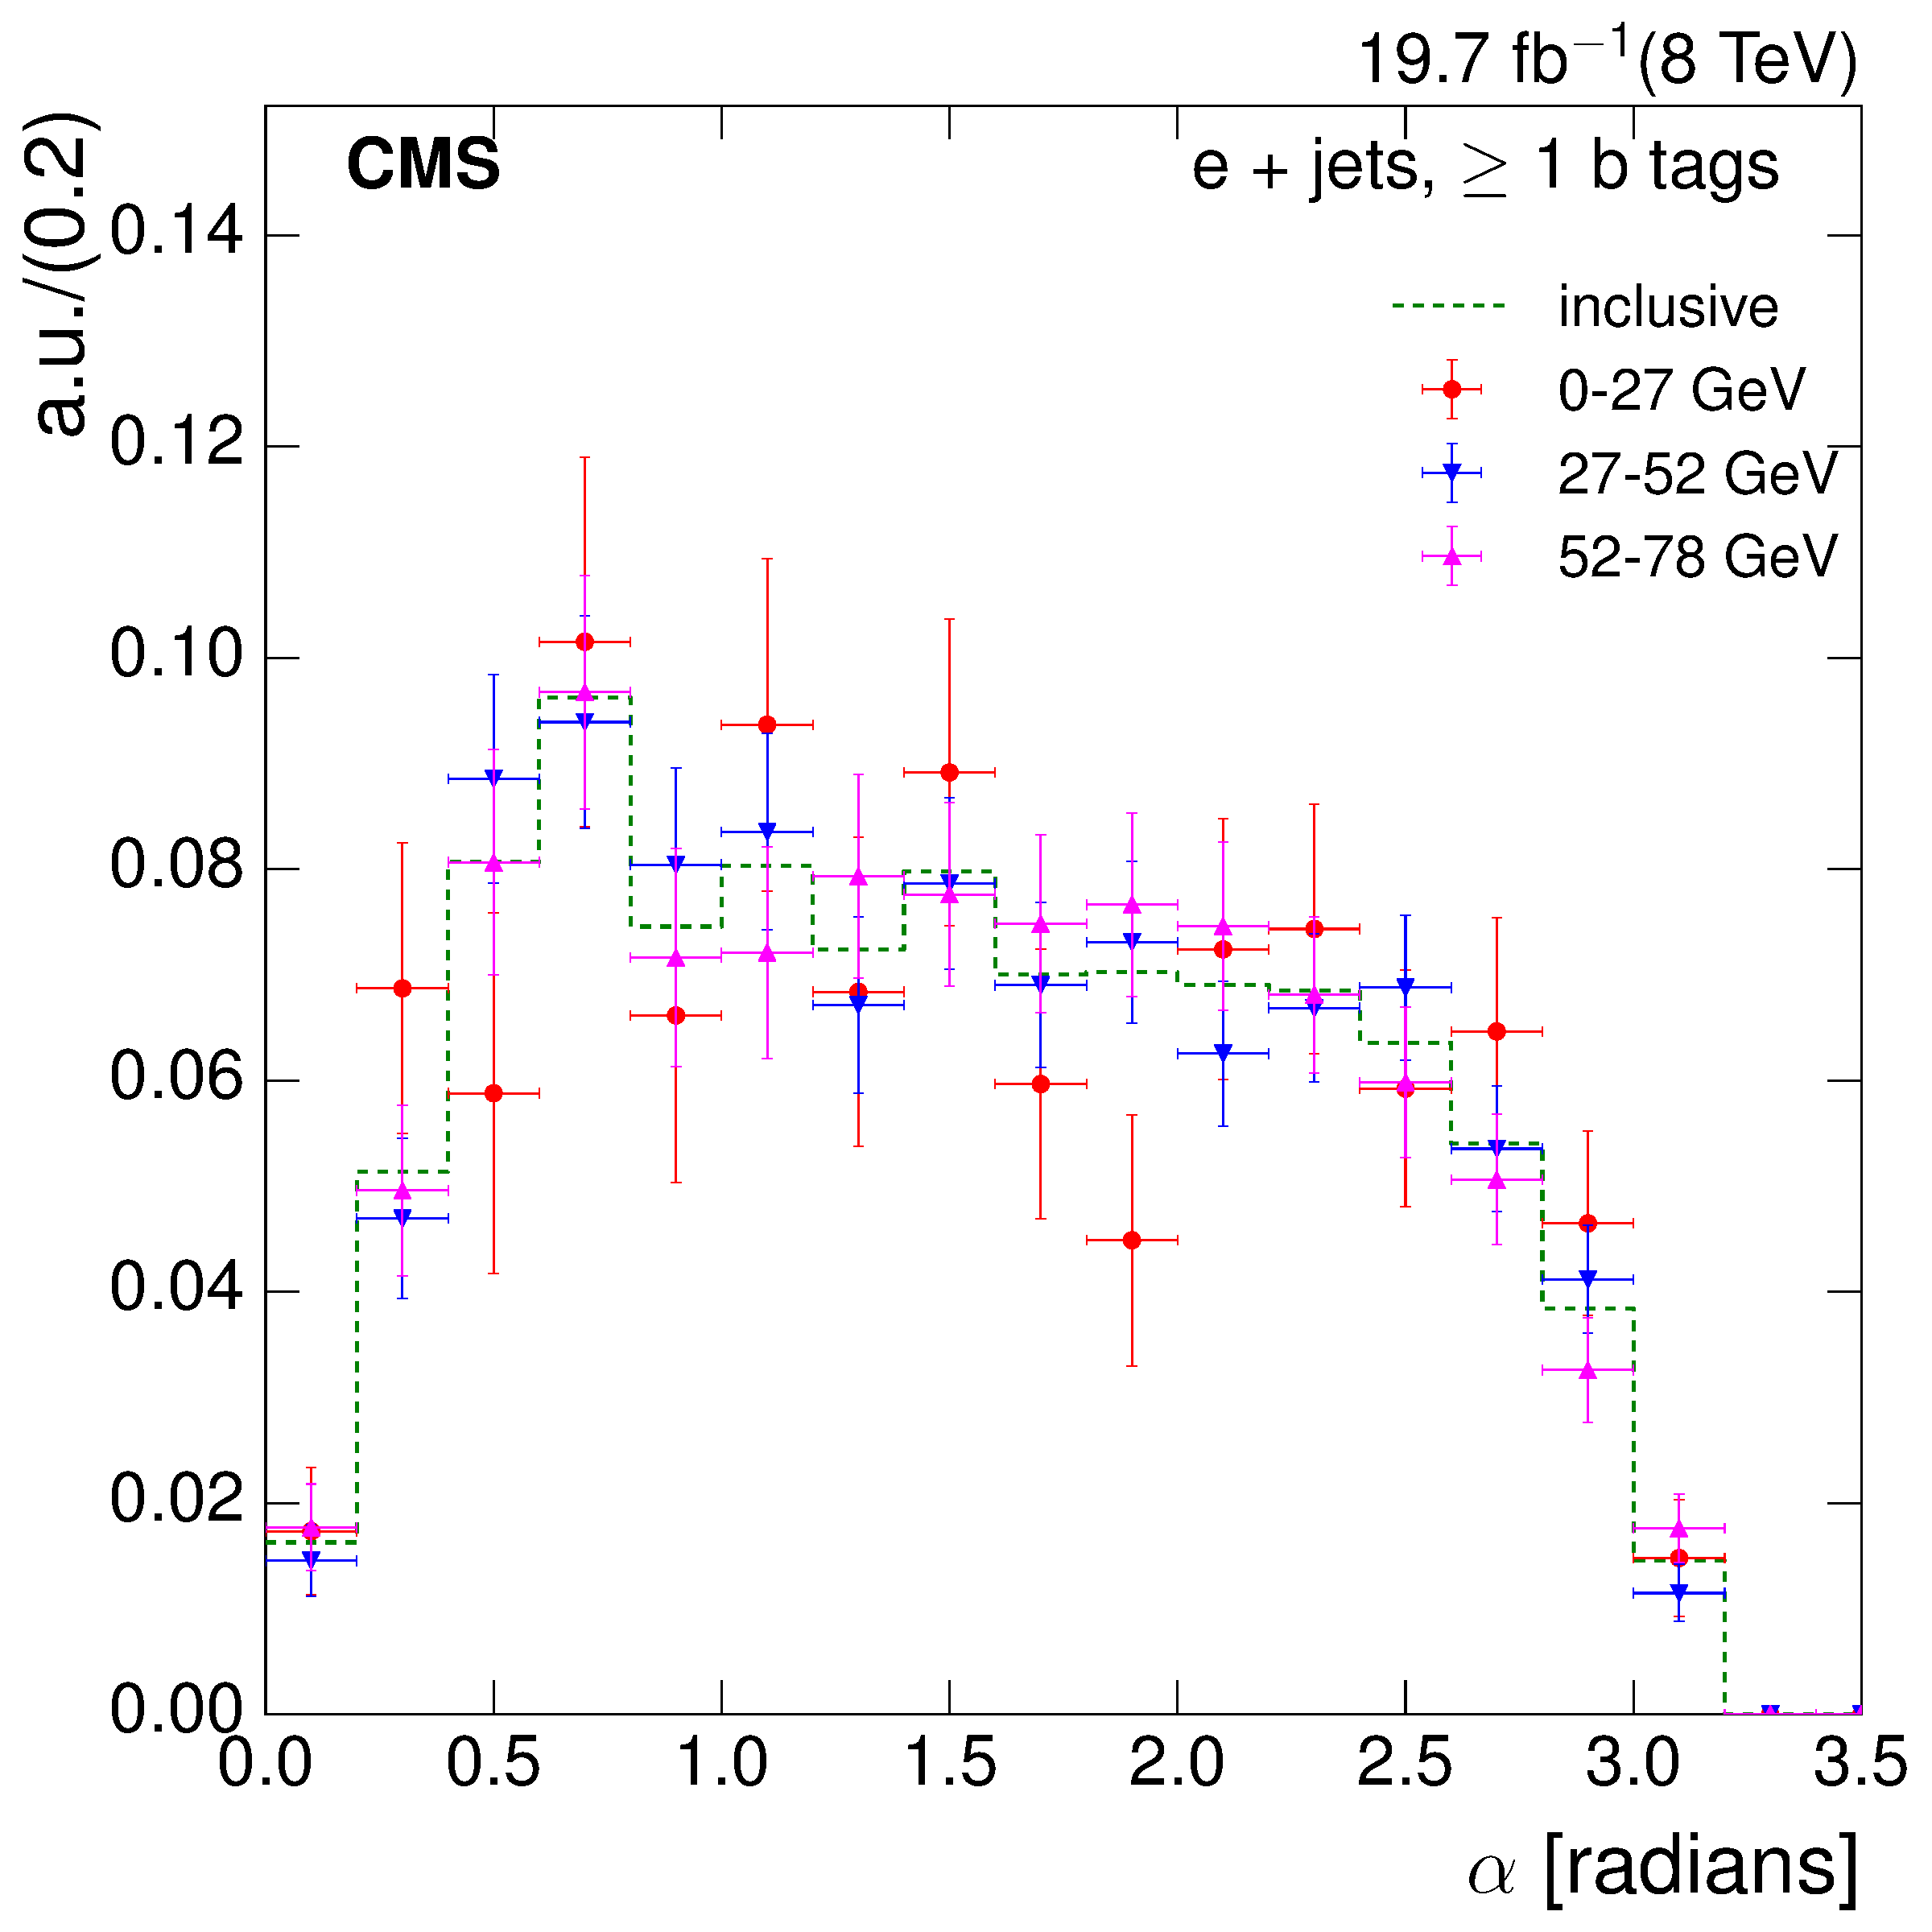
\includegraphics[width=0.48\textwidth]{Chapters/07_08_09_Analysis/Images/8TeV/fit_variables/electron/WPT/angle_bl/qcd/WPT_angle_bl_1orMoreBtag_QCD_template_comparison.pdf}\hfill
%      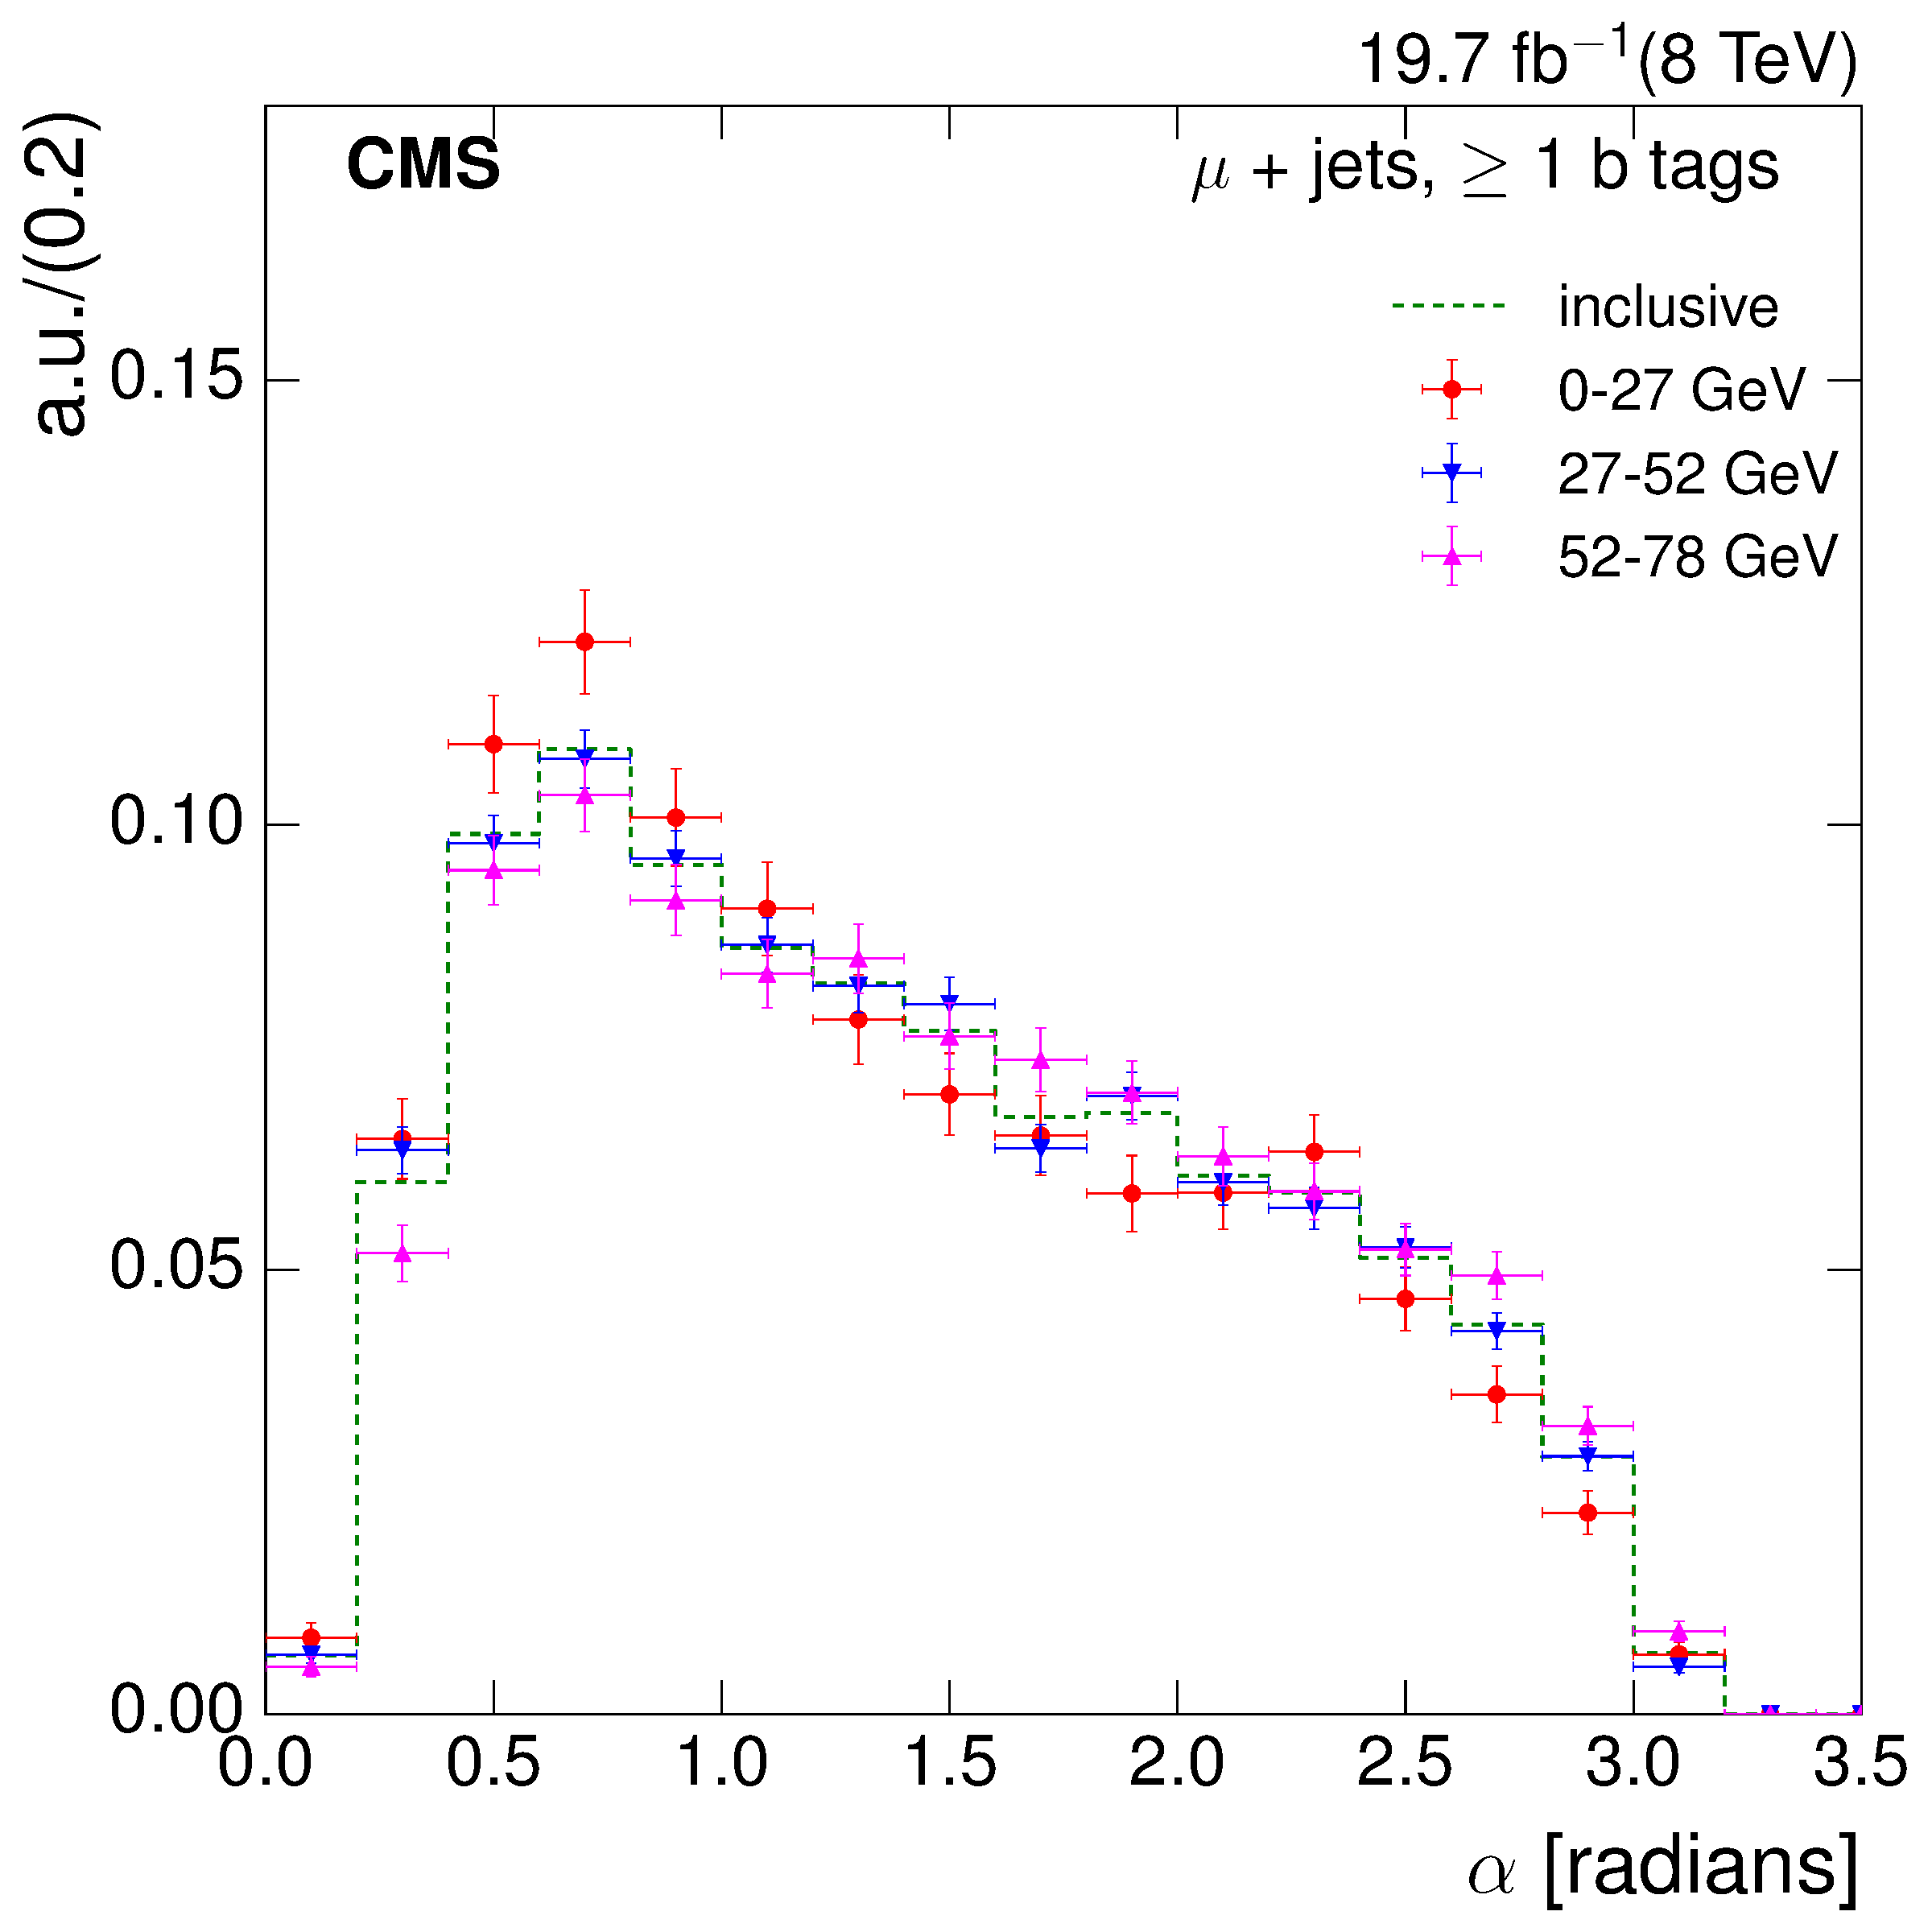
\includegraphics[width=0.48\textwidth]{Chapters/07_08_09_Analysis/Images/8TeV/fit_variables/muon/WPT/angle_bl/qcd/WPT_angle_bl_1orMoreBtag_QCD_template_comparison.pdf}\\
%      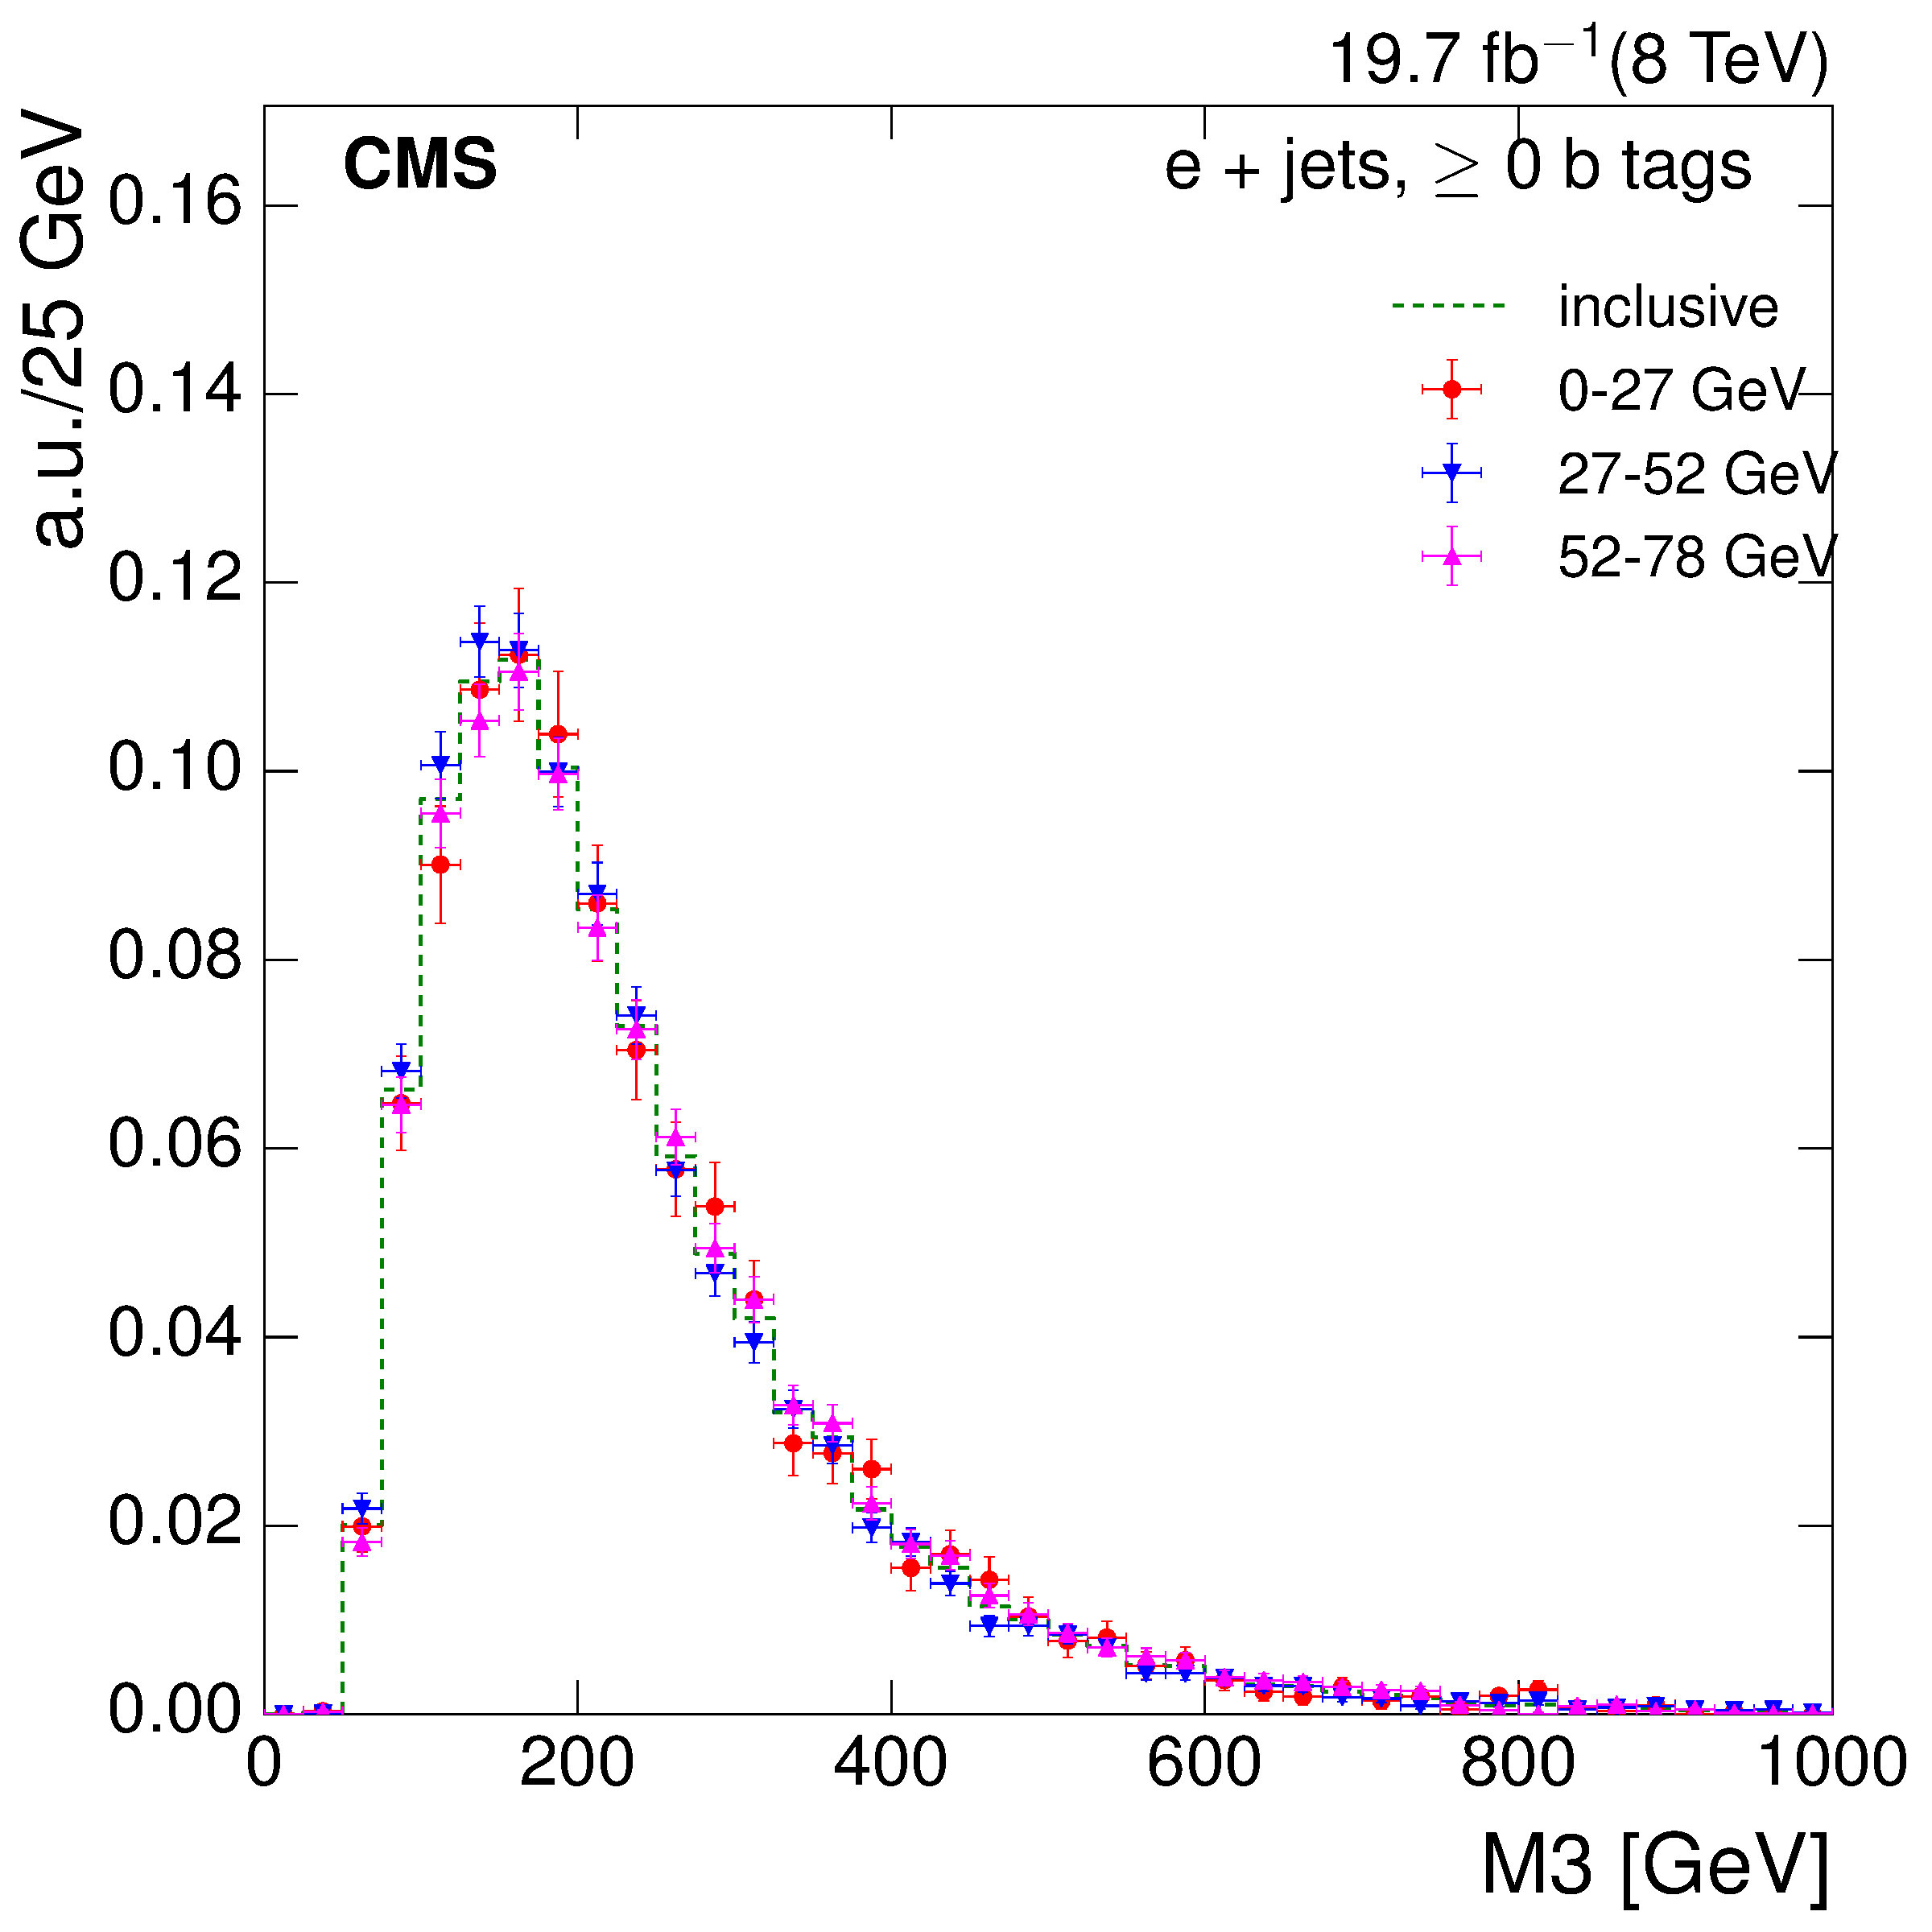
\includegraphics[width=0.48\textwidth]{Chapters/07_08_09_Analysis/Images/8TeV/fit_variables/electron/WPT/M3/qcd/WPT_M3_0orMoreBtag_QCD_template_comparison.pdf}\hfill
%      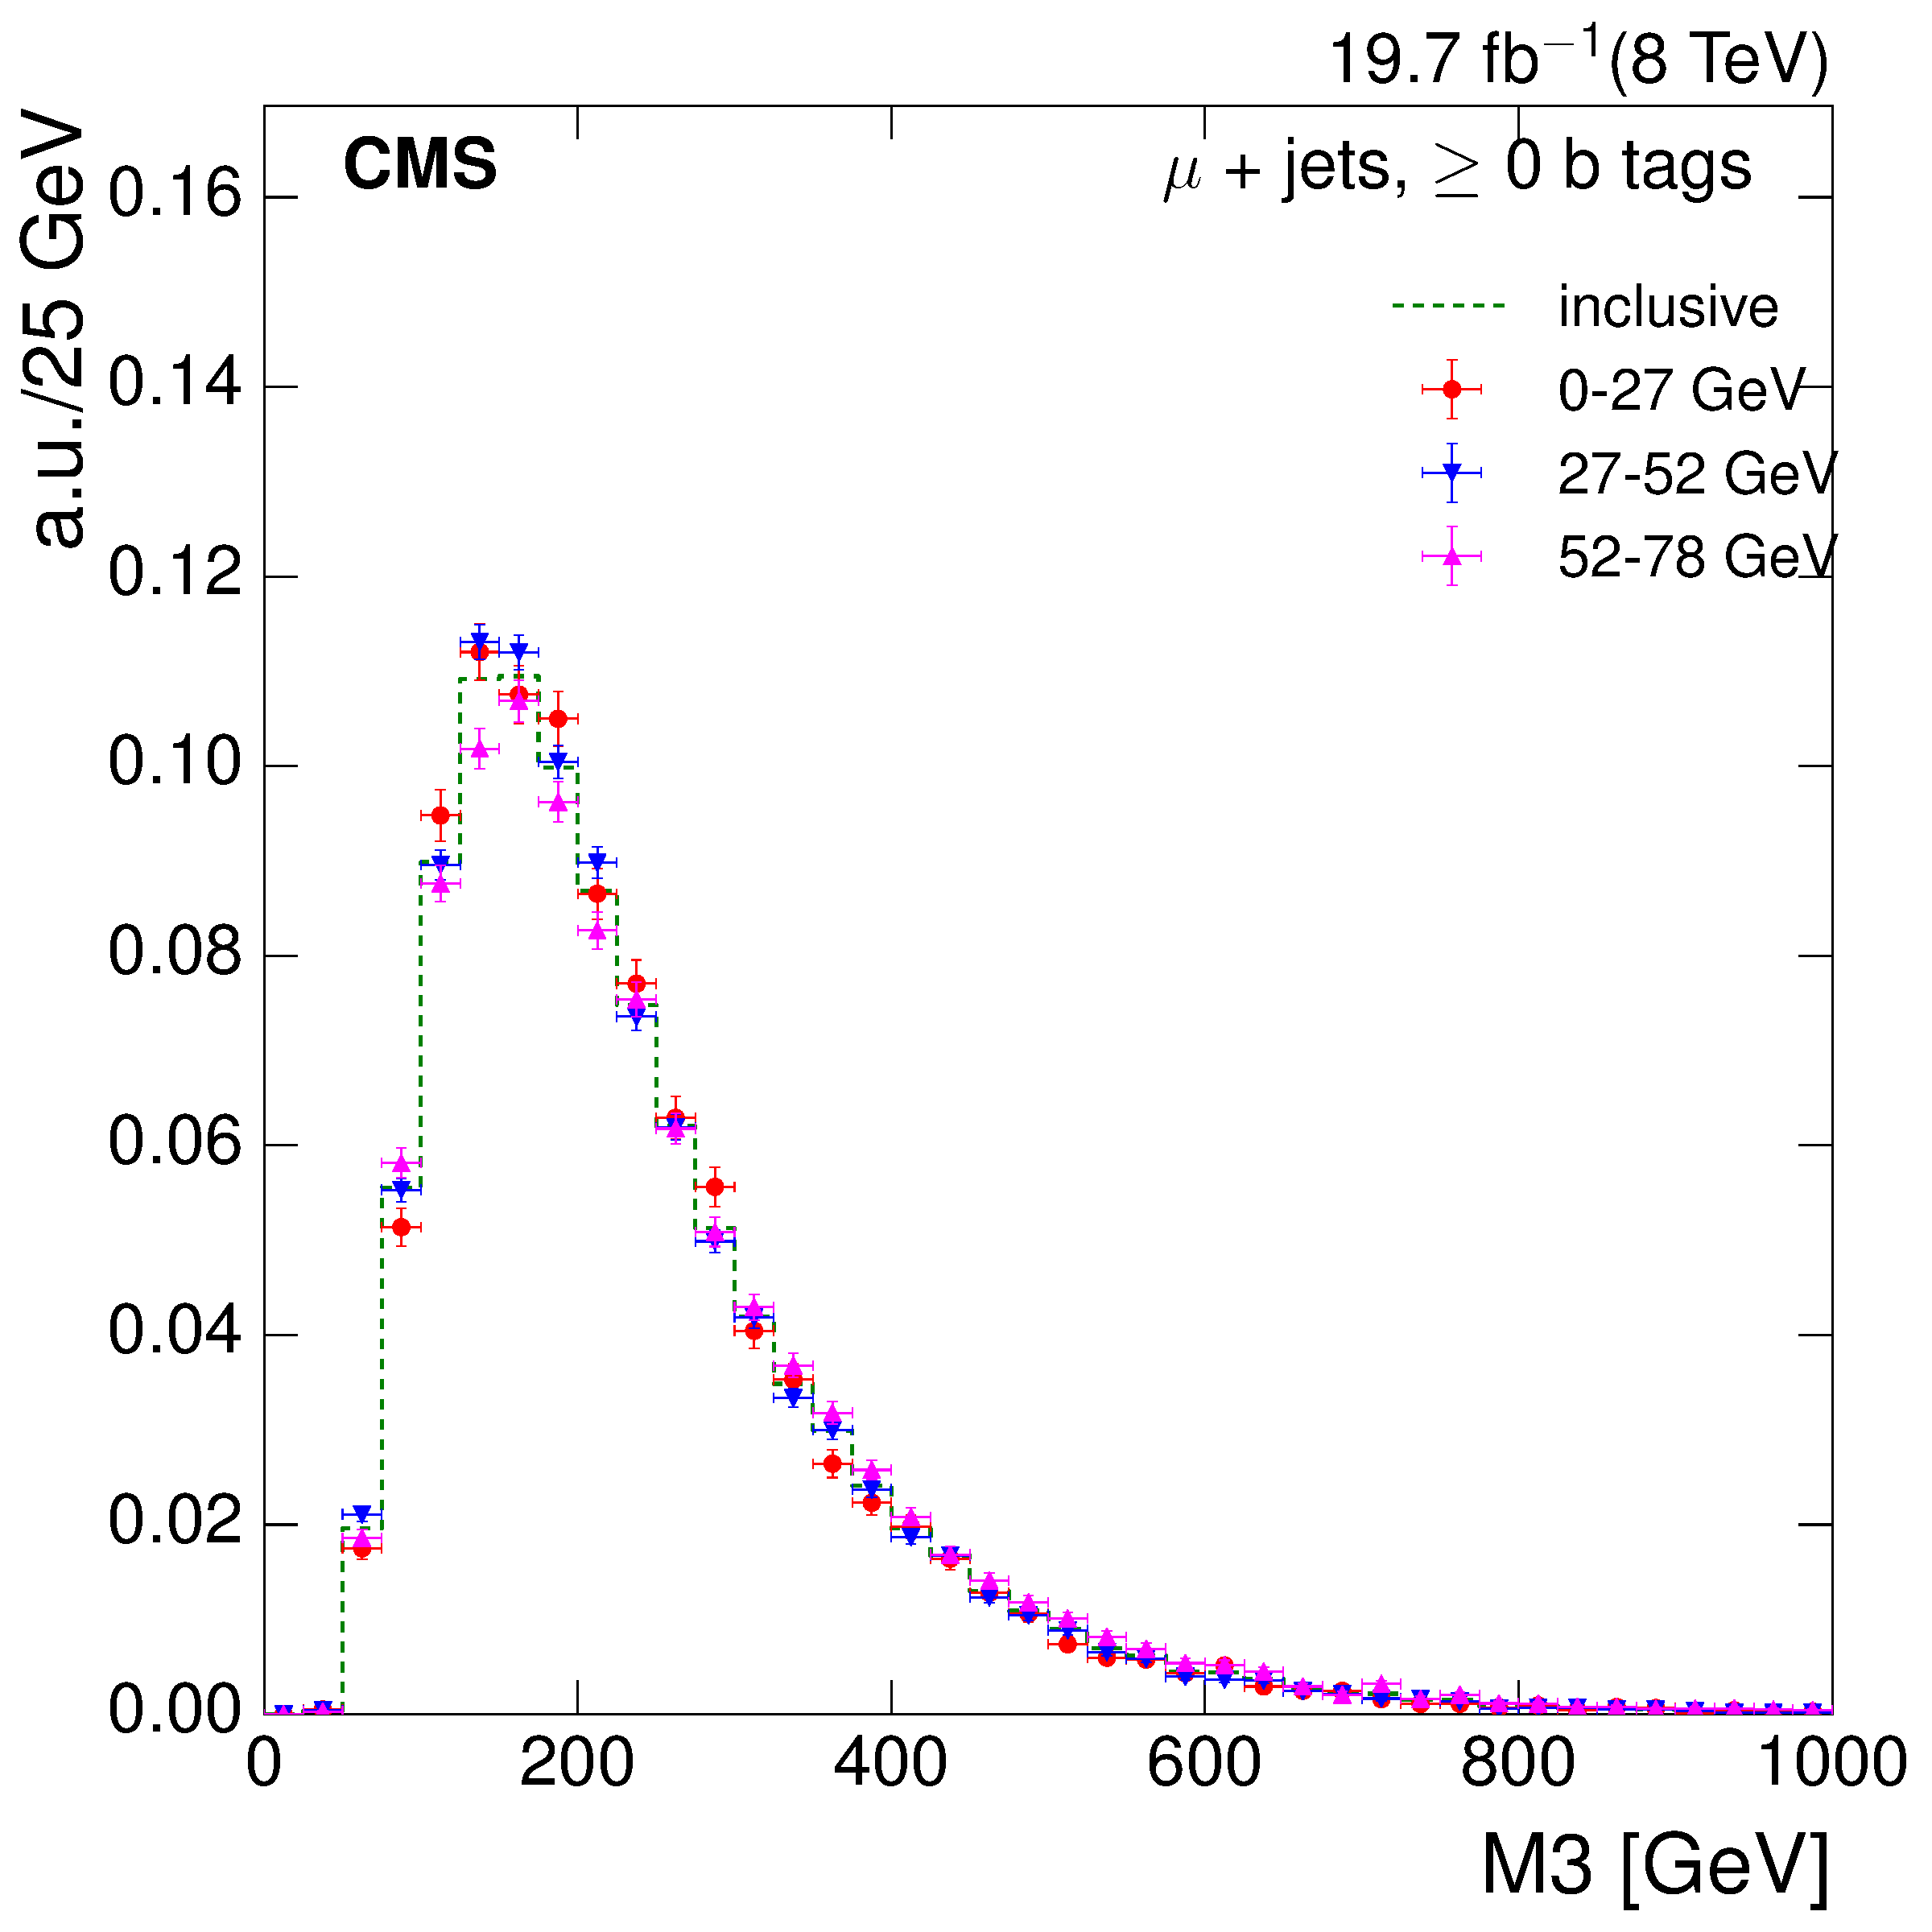
\includegraphics[width=0.48\textwidth]{Chapters/07_08_09_Analysis/Images/8TeV/fit_variables/muon/WPT/M3/qcd/WPT_M3_0orMoreBtag_QCD_template_comparison.pdf}\\
% 	 \caption[Normalised distributions of the QCD templates for the three fit variables in \wpt bins
% 	 at $\sqrt{s}=8\TeV$.]{Normalised distributions of the QCD templates for the three fit variables lepton
% 	 \abseta (upper), $\alpha$ (middle) and M3 (lower) inclusive across all \wpt bins and for the lowest three \wpt bins at $\sqrt{s}=8\TeV$ in the electron+jets channel (left) and in the muon+jets channel (right).}
%      \label{fig:WPT_fit_variable_qcd_comparisons_8TeV}
% \end{figure}
% 
% \clearpage


% \section{Fitting variable V+jets background template comparisons}
% \label{as:fitting_variable_vjets_template_comparisons}
% 
% \begin{figure}[hbtp]
%     \centering
%      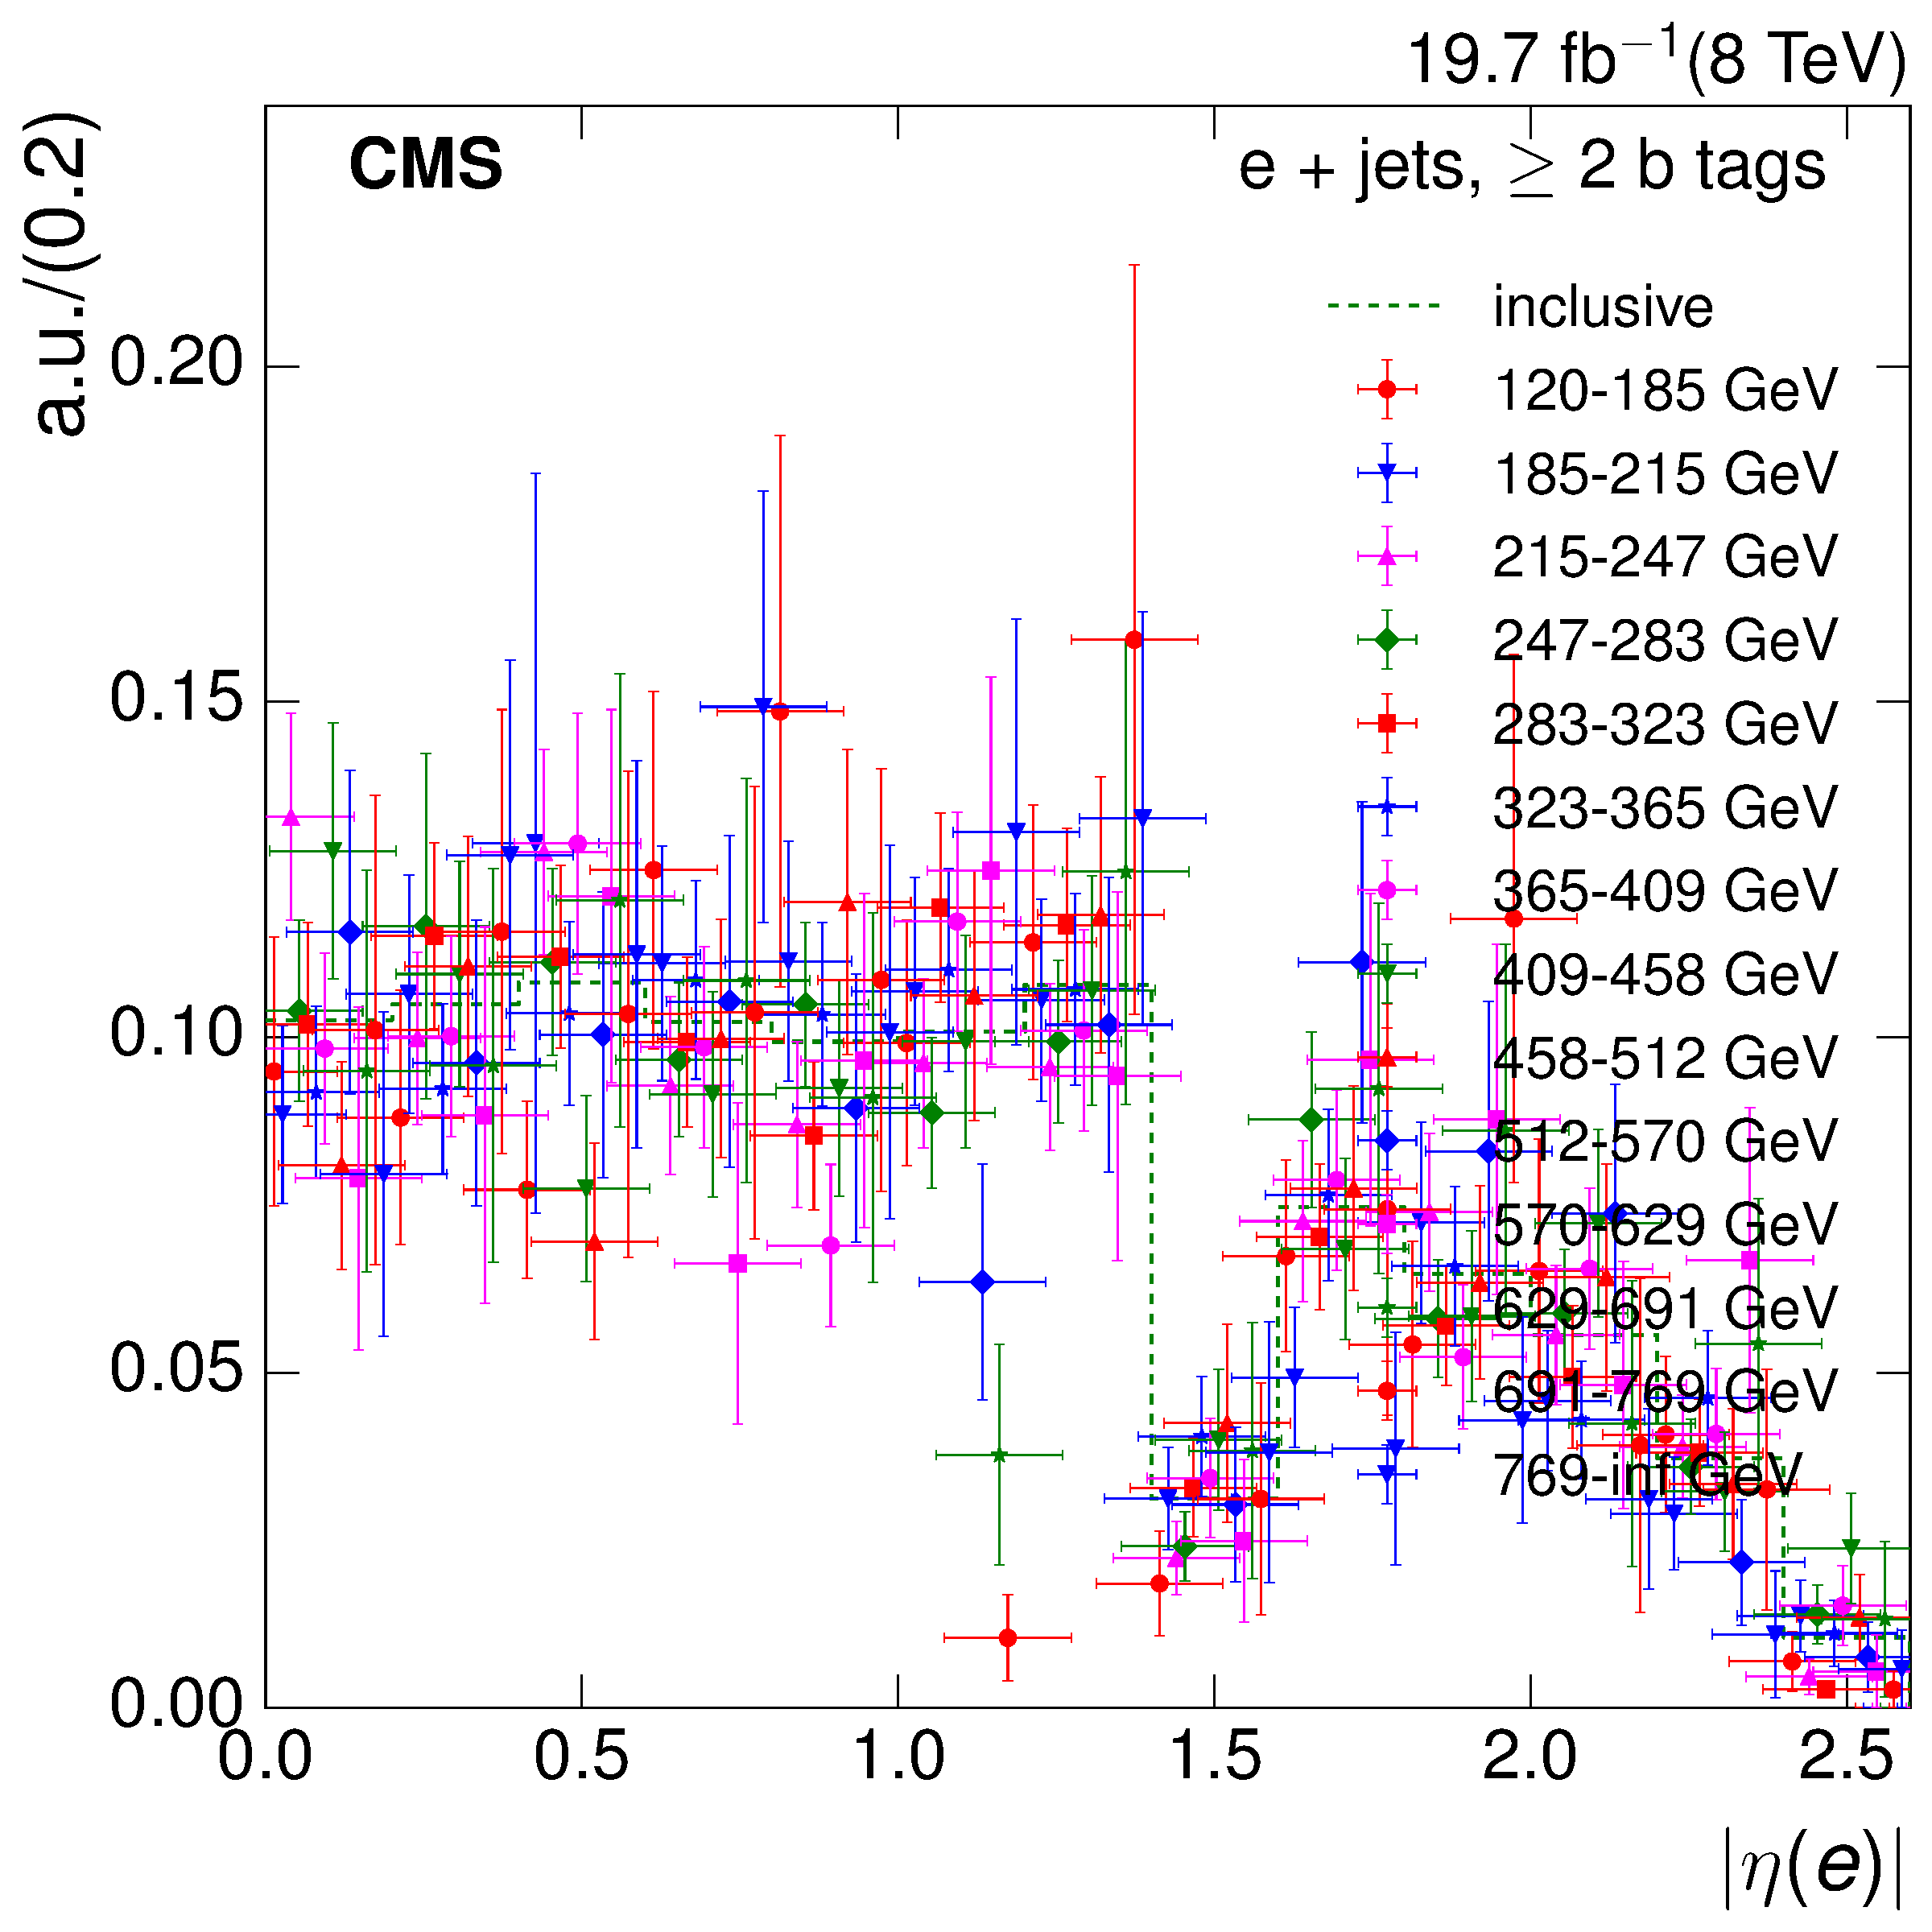
\includegraphics[width=0.48\textwidth]{Chapters/07_08_09_Analysis/Images/8TeV/fit_variables/electron/HT/electron_absolute_eta/vjets/HT_electron_absolute_eta_2orMoreBtags_VJets_template_comparison.pdf}\hfill
%      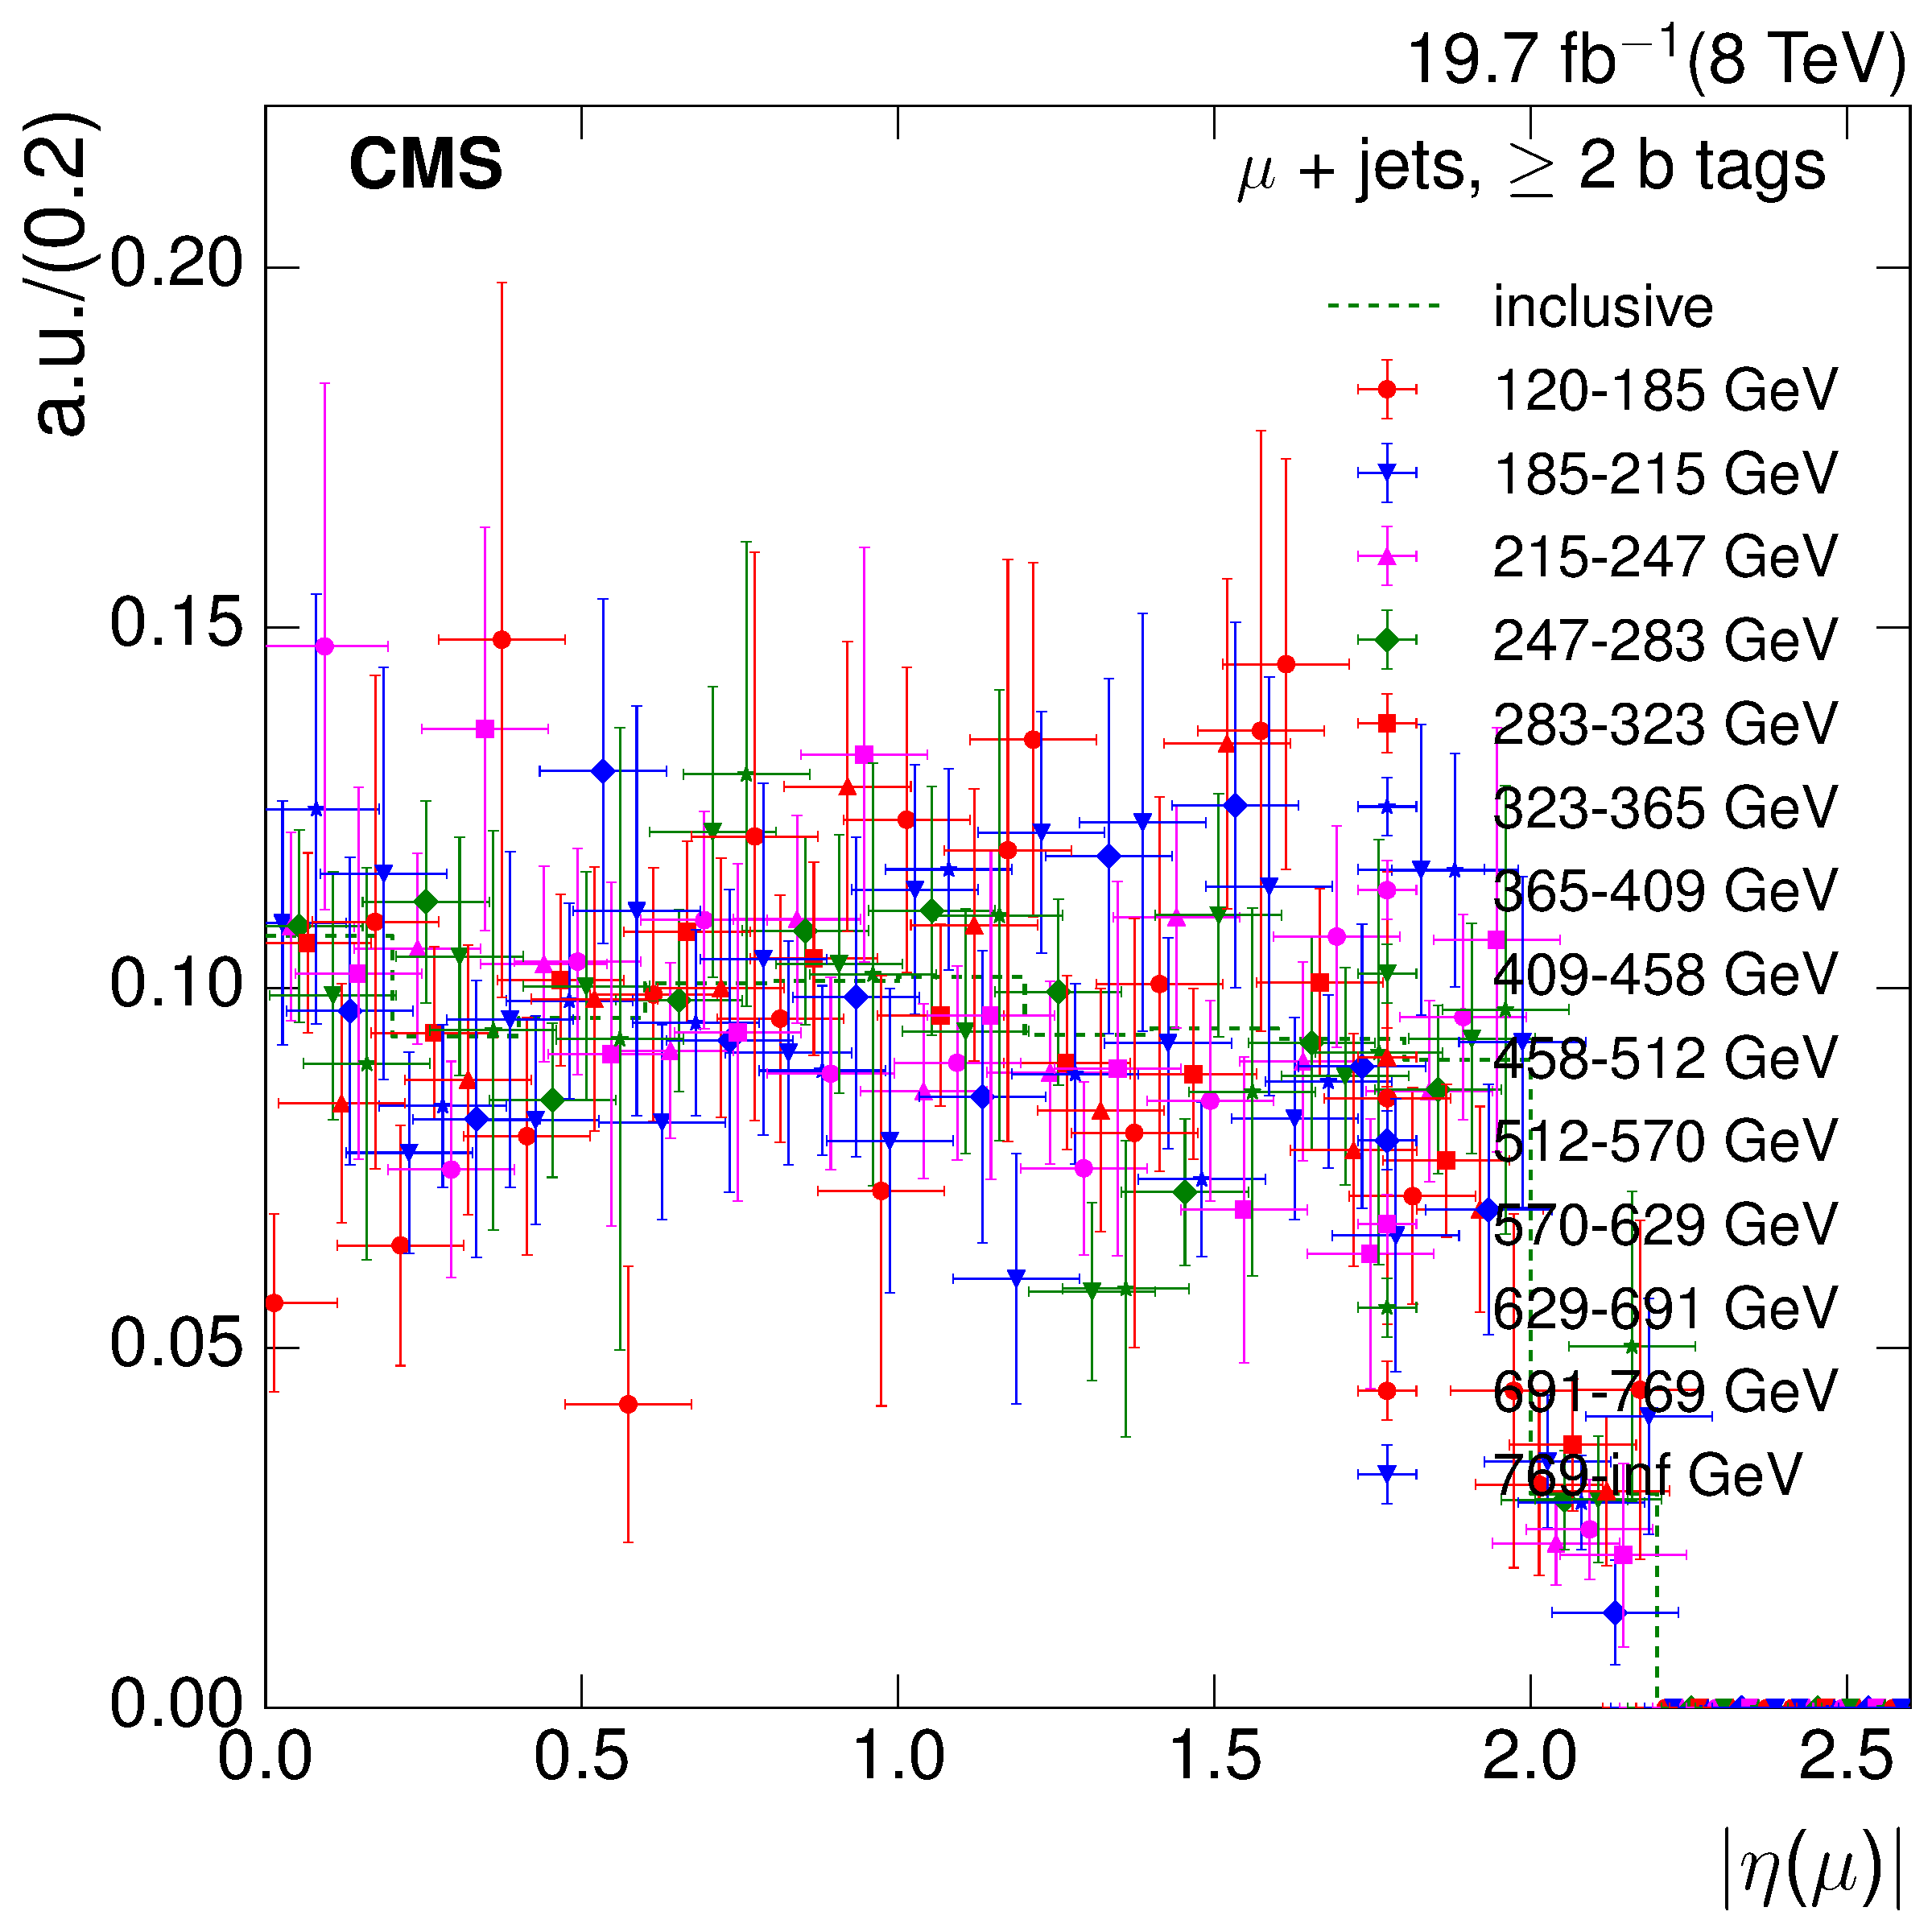
\includegraphics[width=0.48\textwidth]{Chapters/07_08_09_Analysis/Images/8TeV/fit_variables/muon/HT/muon_absolute_eta/vjets/HT_muon_absolute_eta_2orMoreBtags_VJets_template_comparison.pdf}\\
%      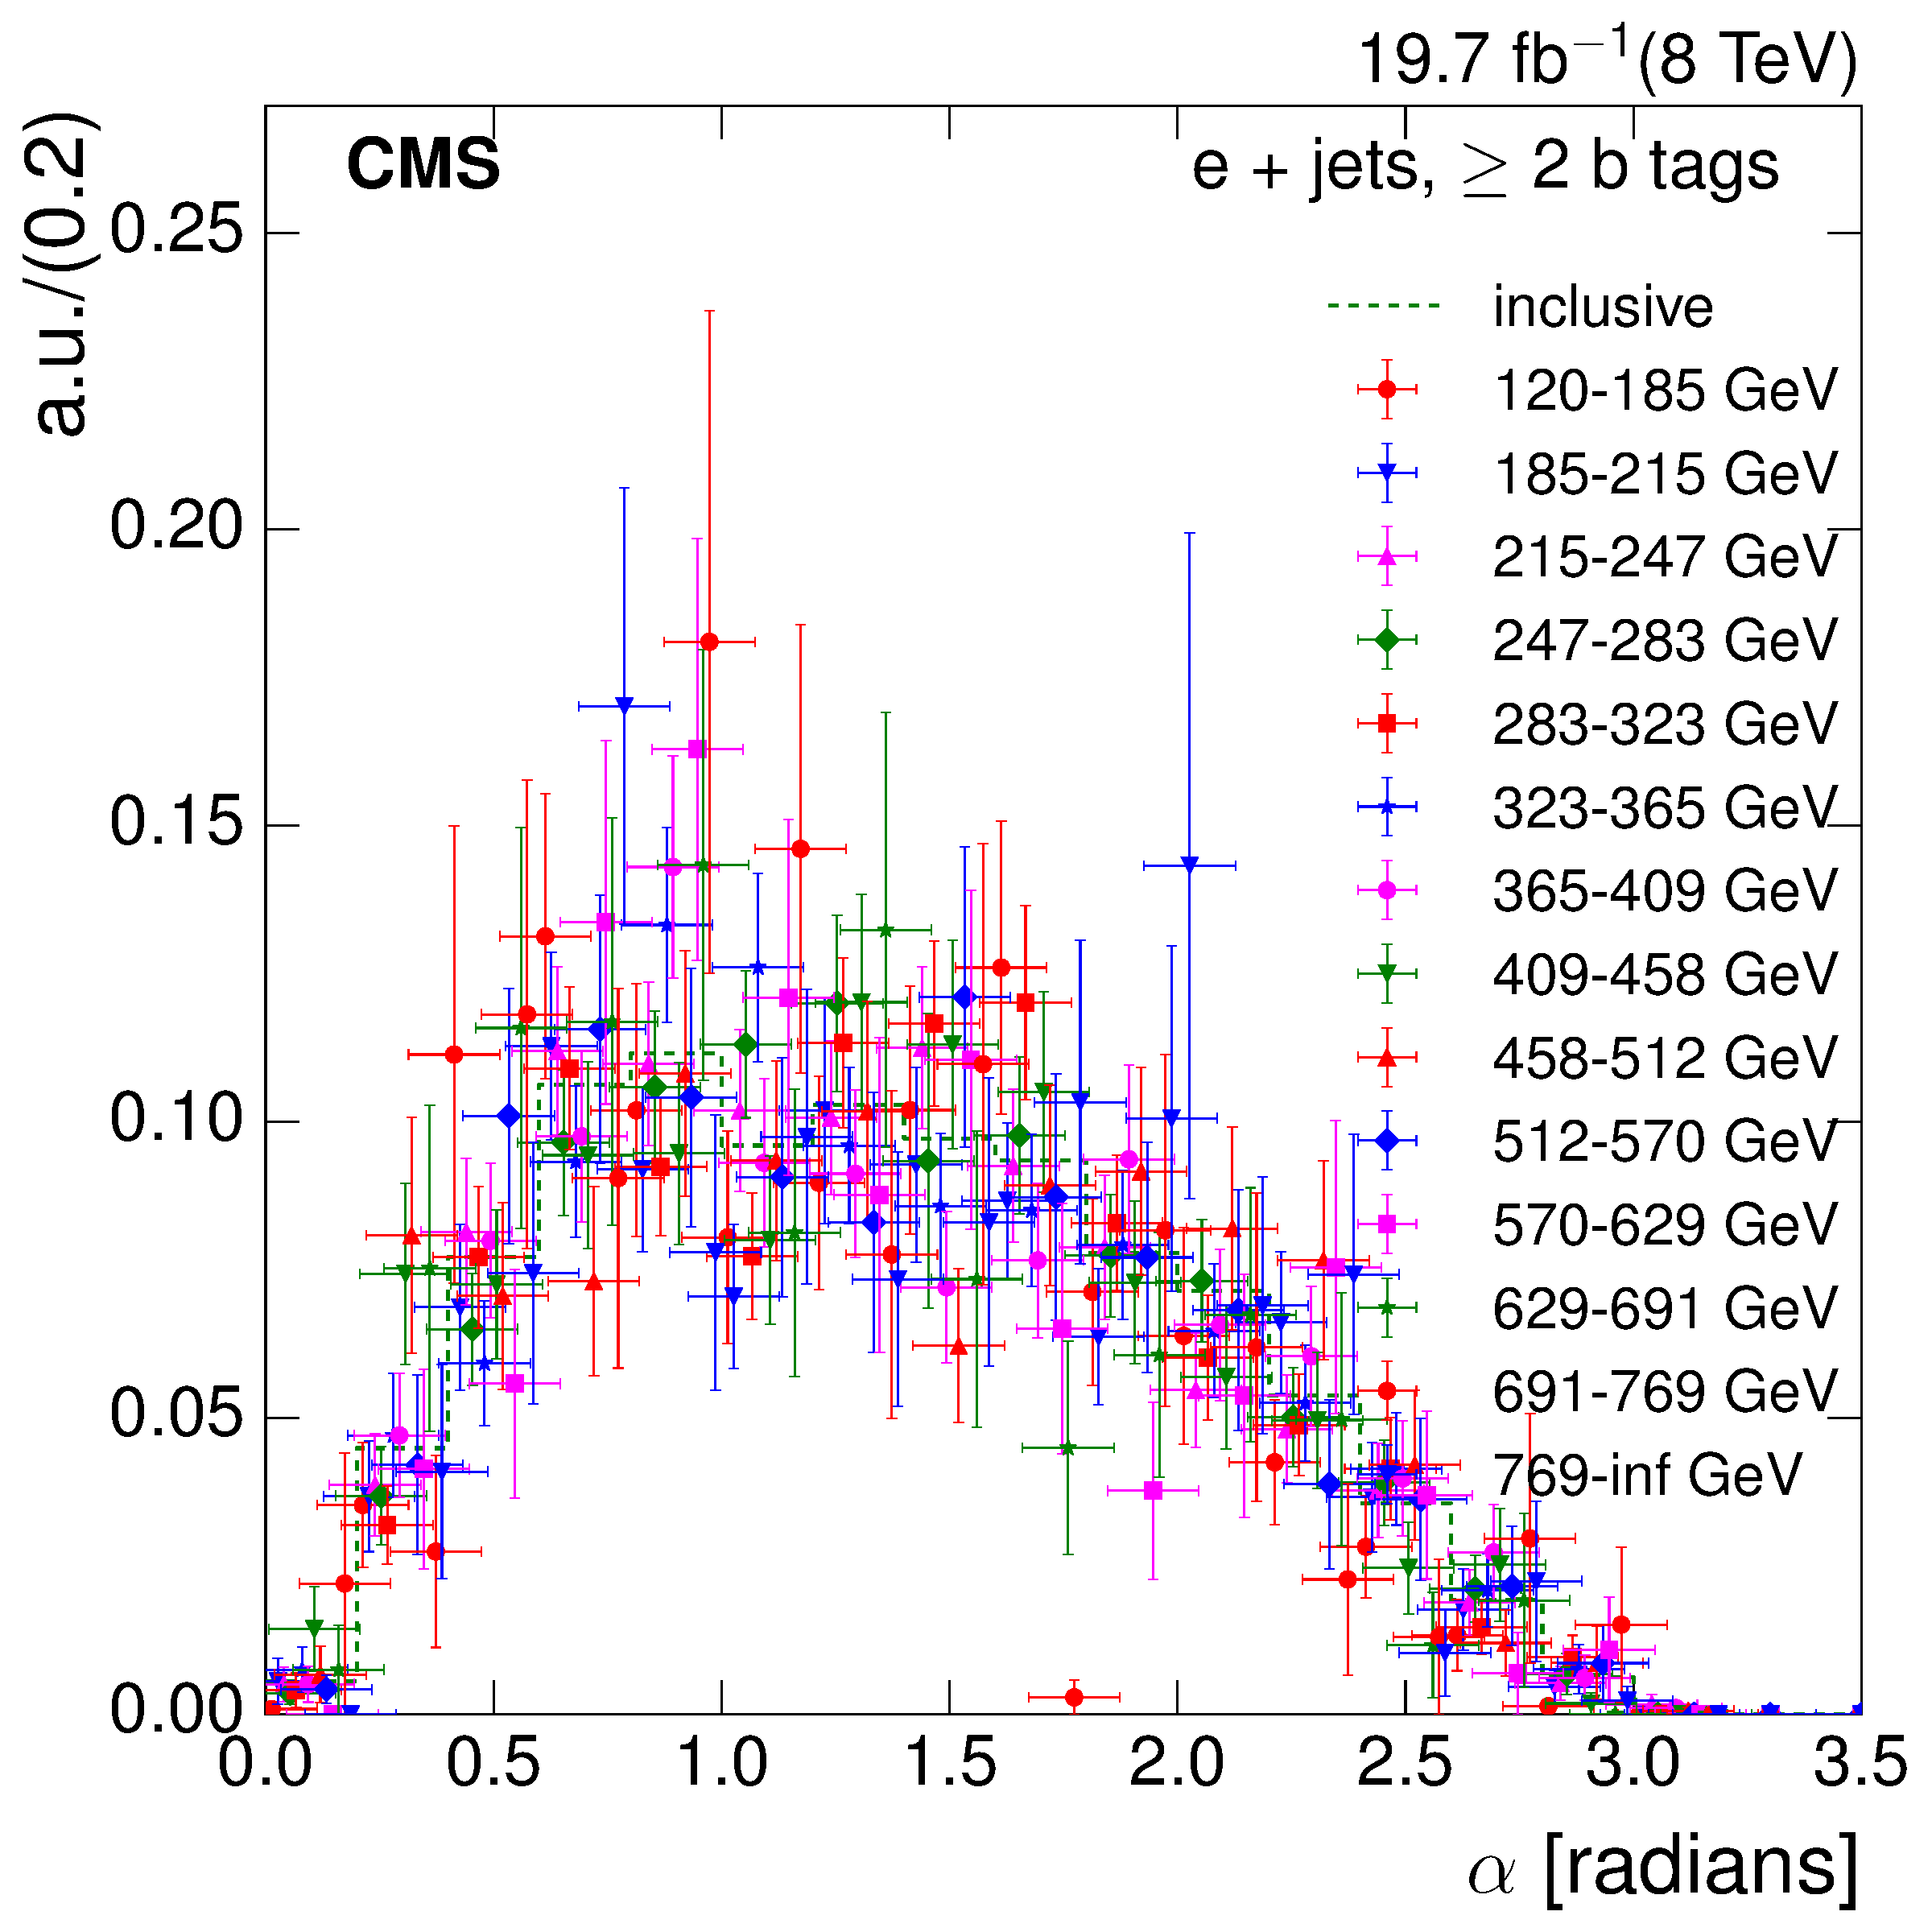
\includegraphics[width=0.48\textwidth]{Chapters/07_08_09_Analysis/Images/8TeV/fit_variables/electron/HT/angle_bl/vjets/HT_angle_bl_2orMoreBtags_VJets_template_comparison.pdf}\hfill
%      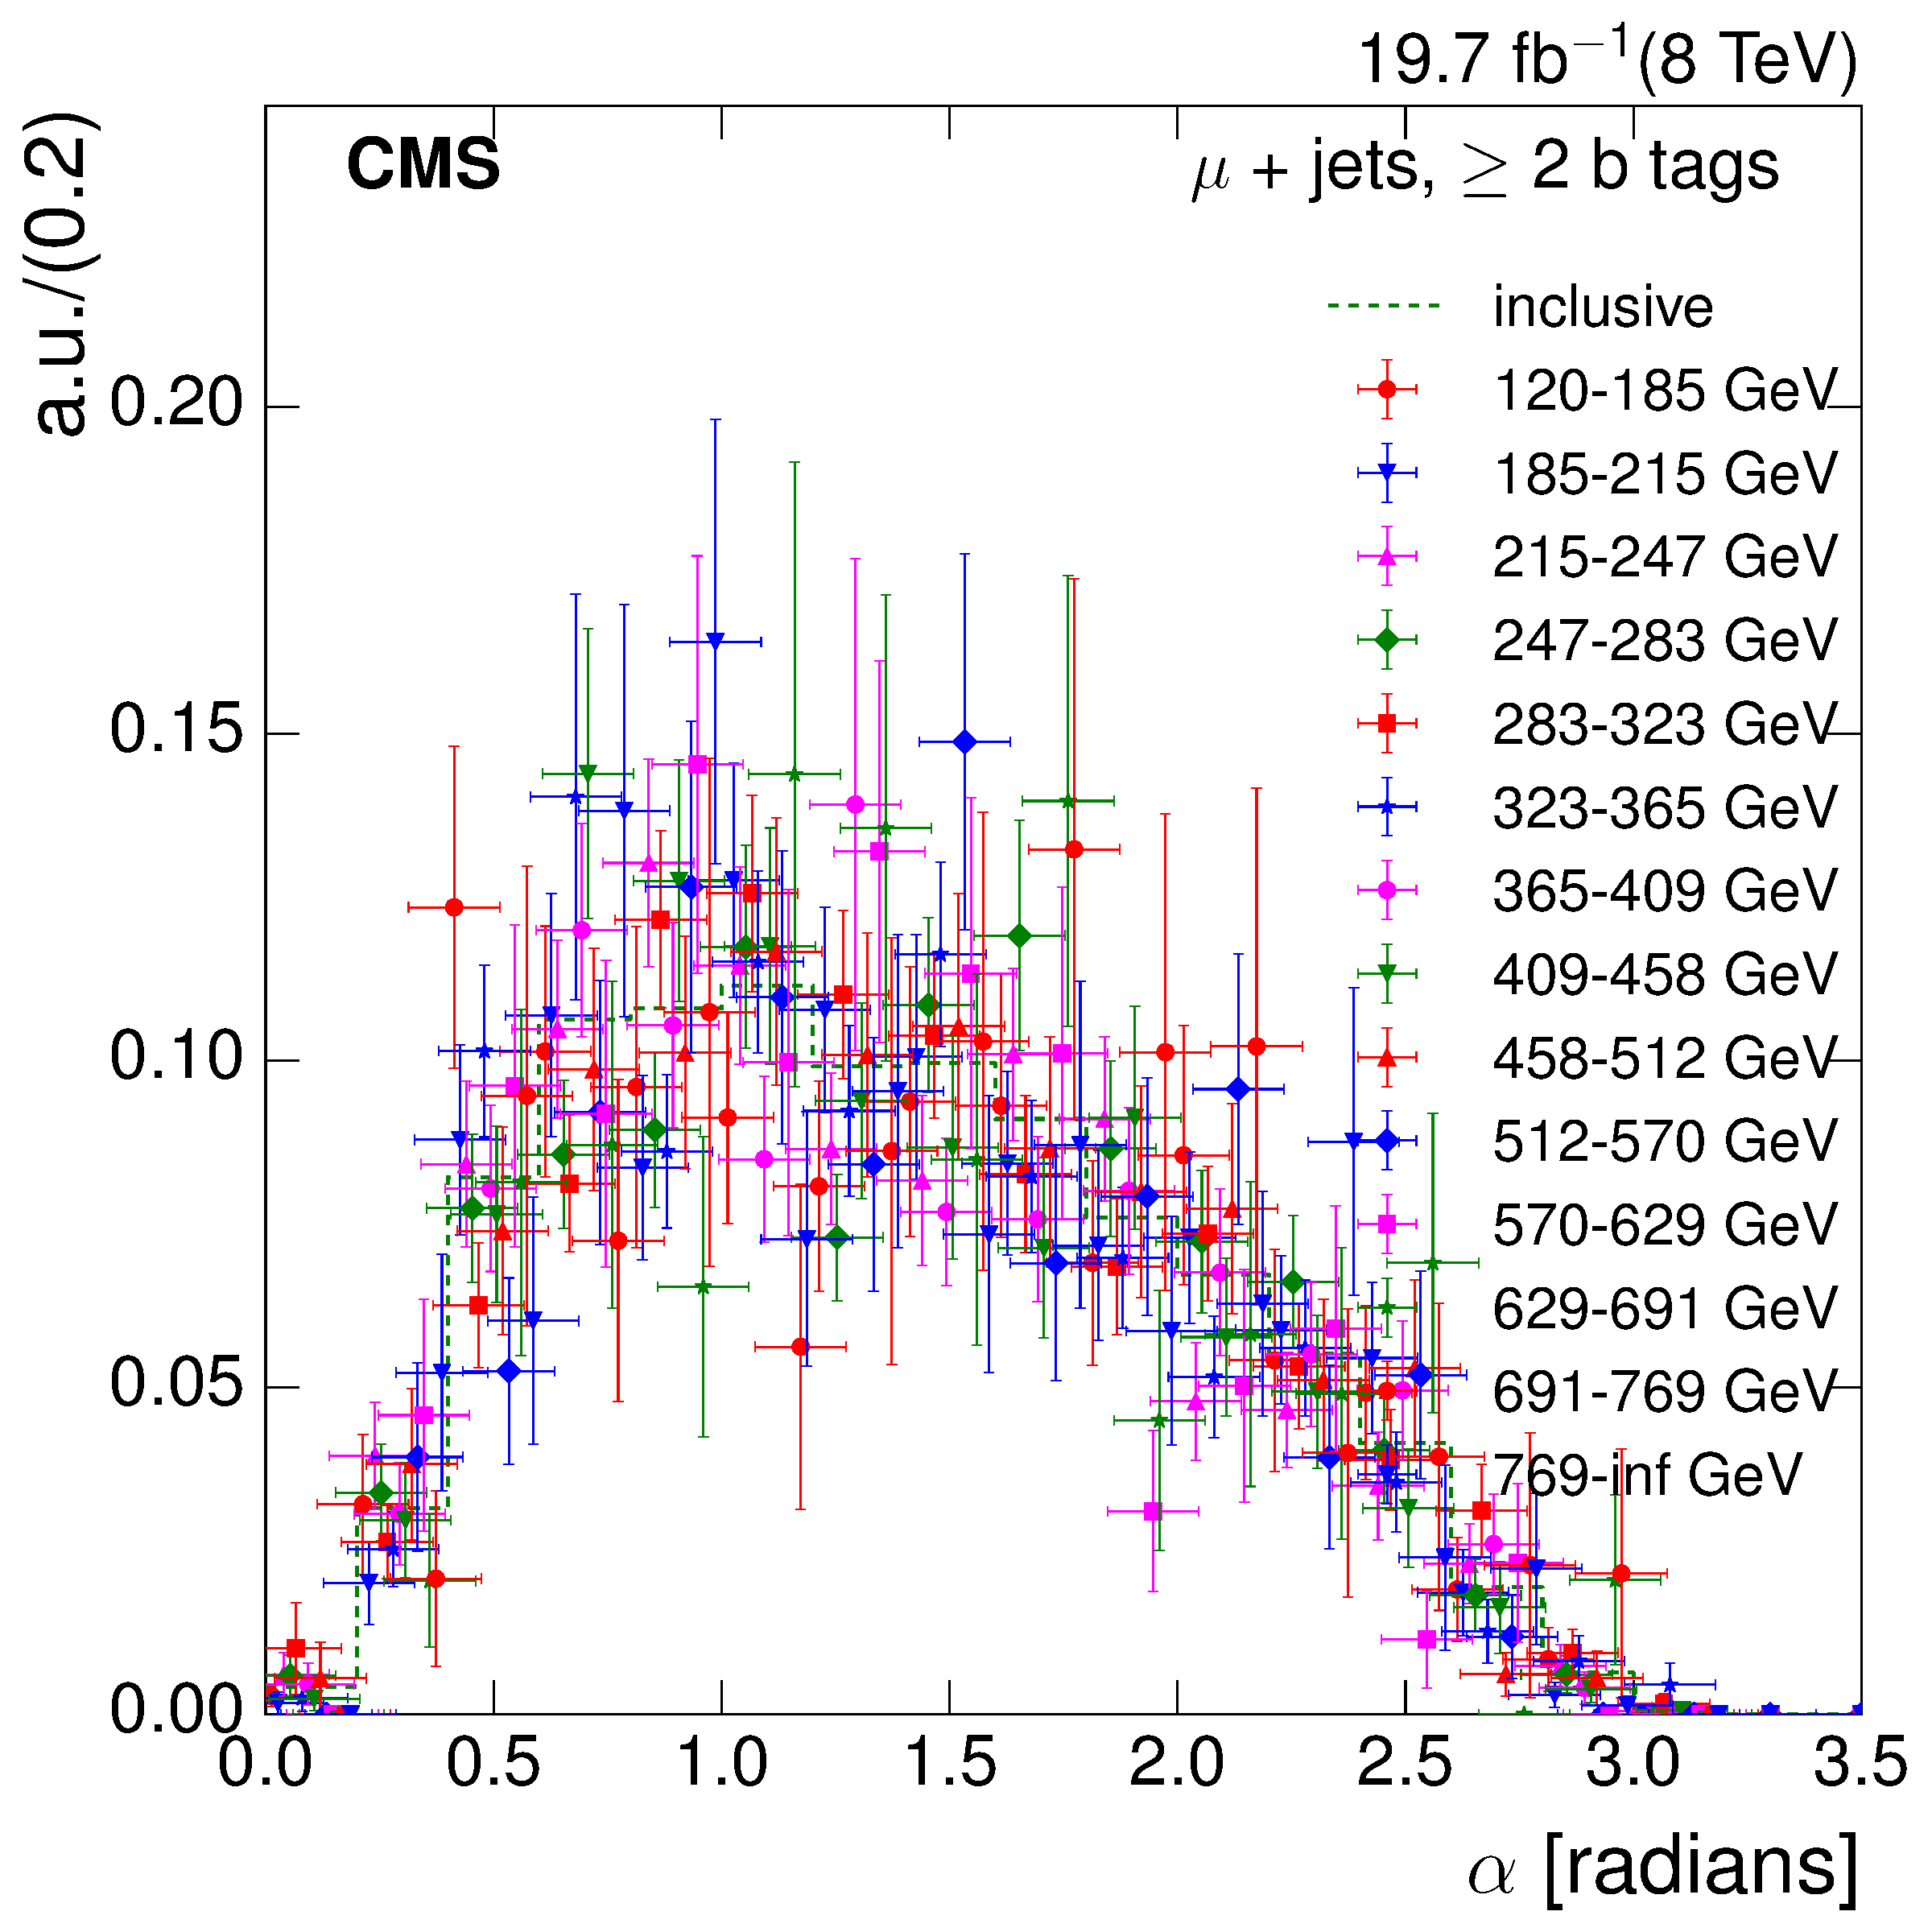
\includegraphics[width=0.48\textwidth]{Chapters/07_08_09_Analysis/Images/8TeV/fit_variables/muon/HT/angle_bl/vjets/HT_angle_bl_2orMoreBtags_VJets_template_comparison.pdf}\\
%      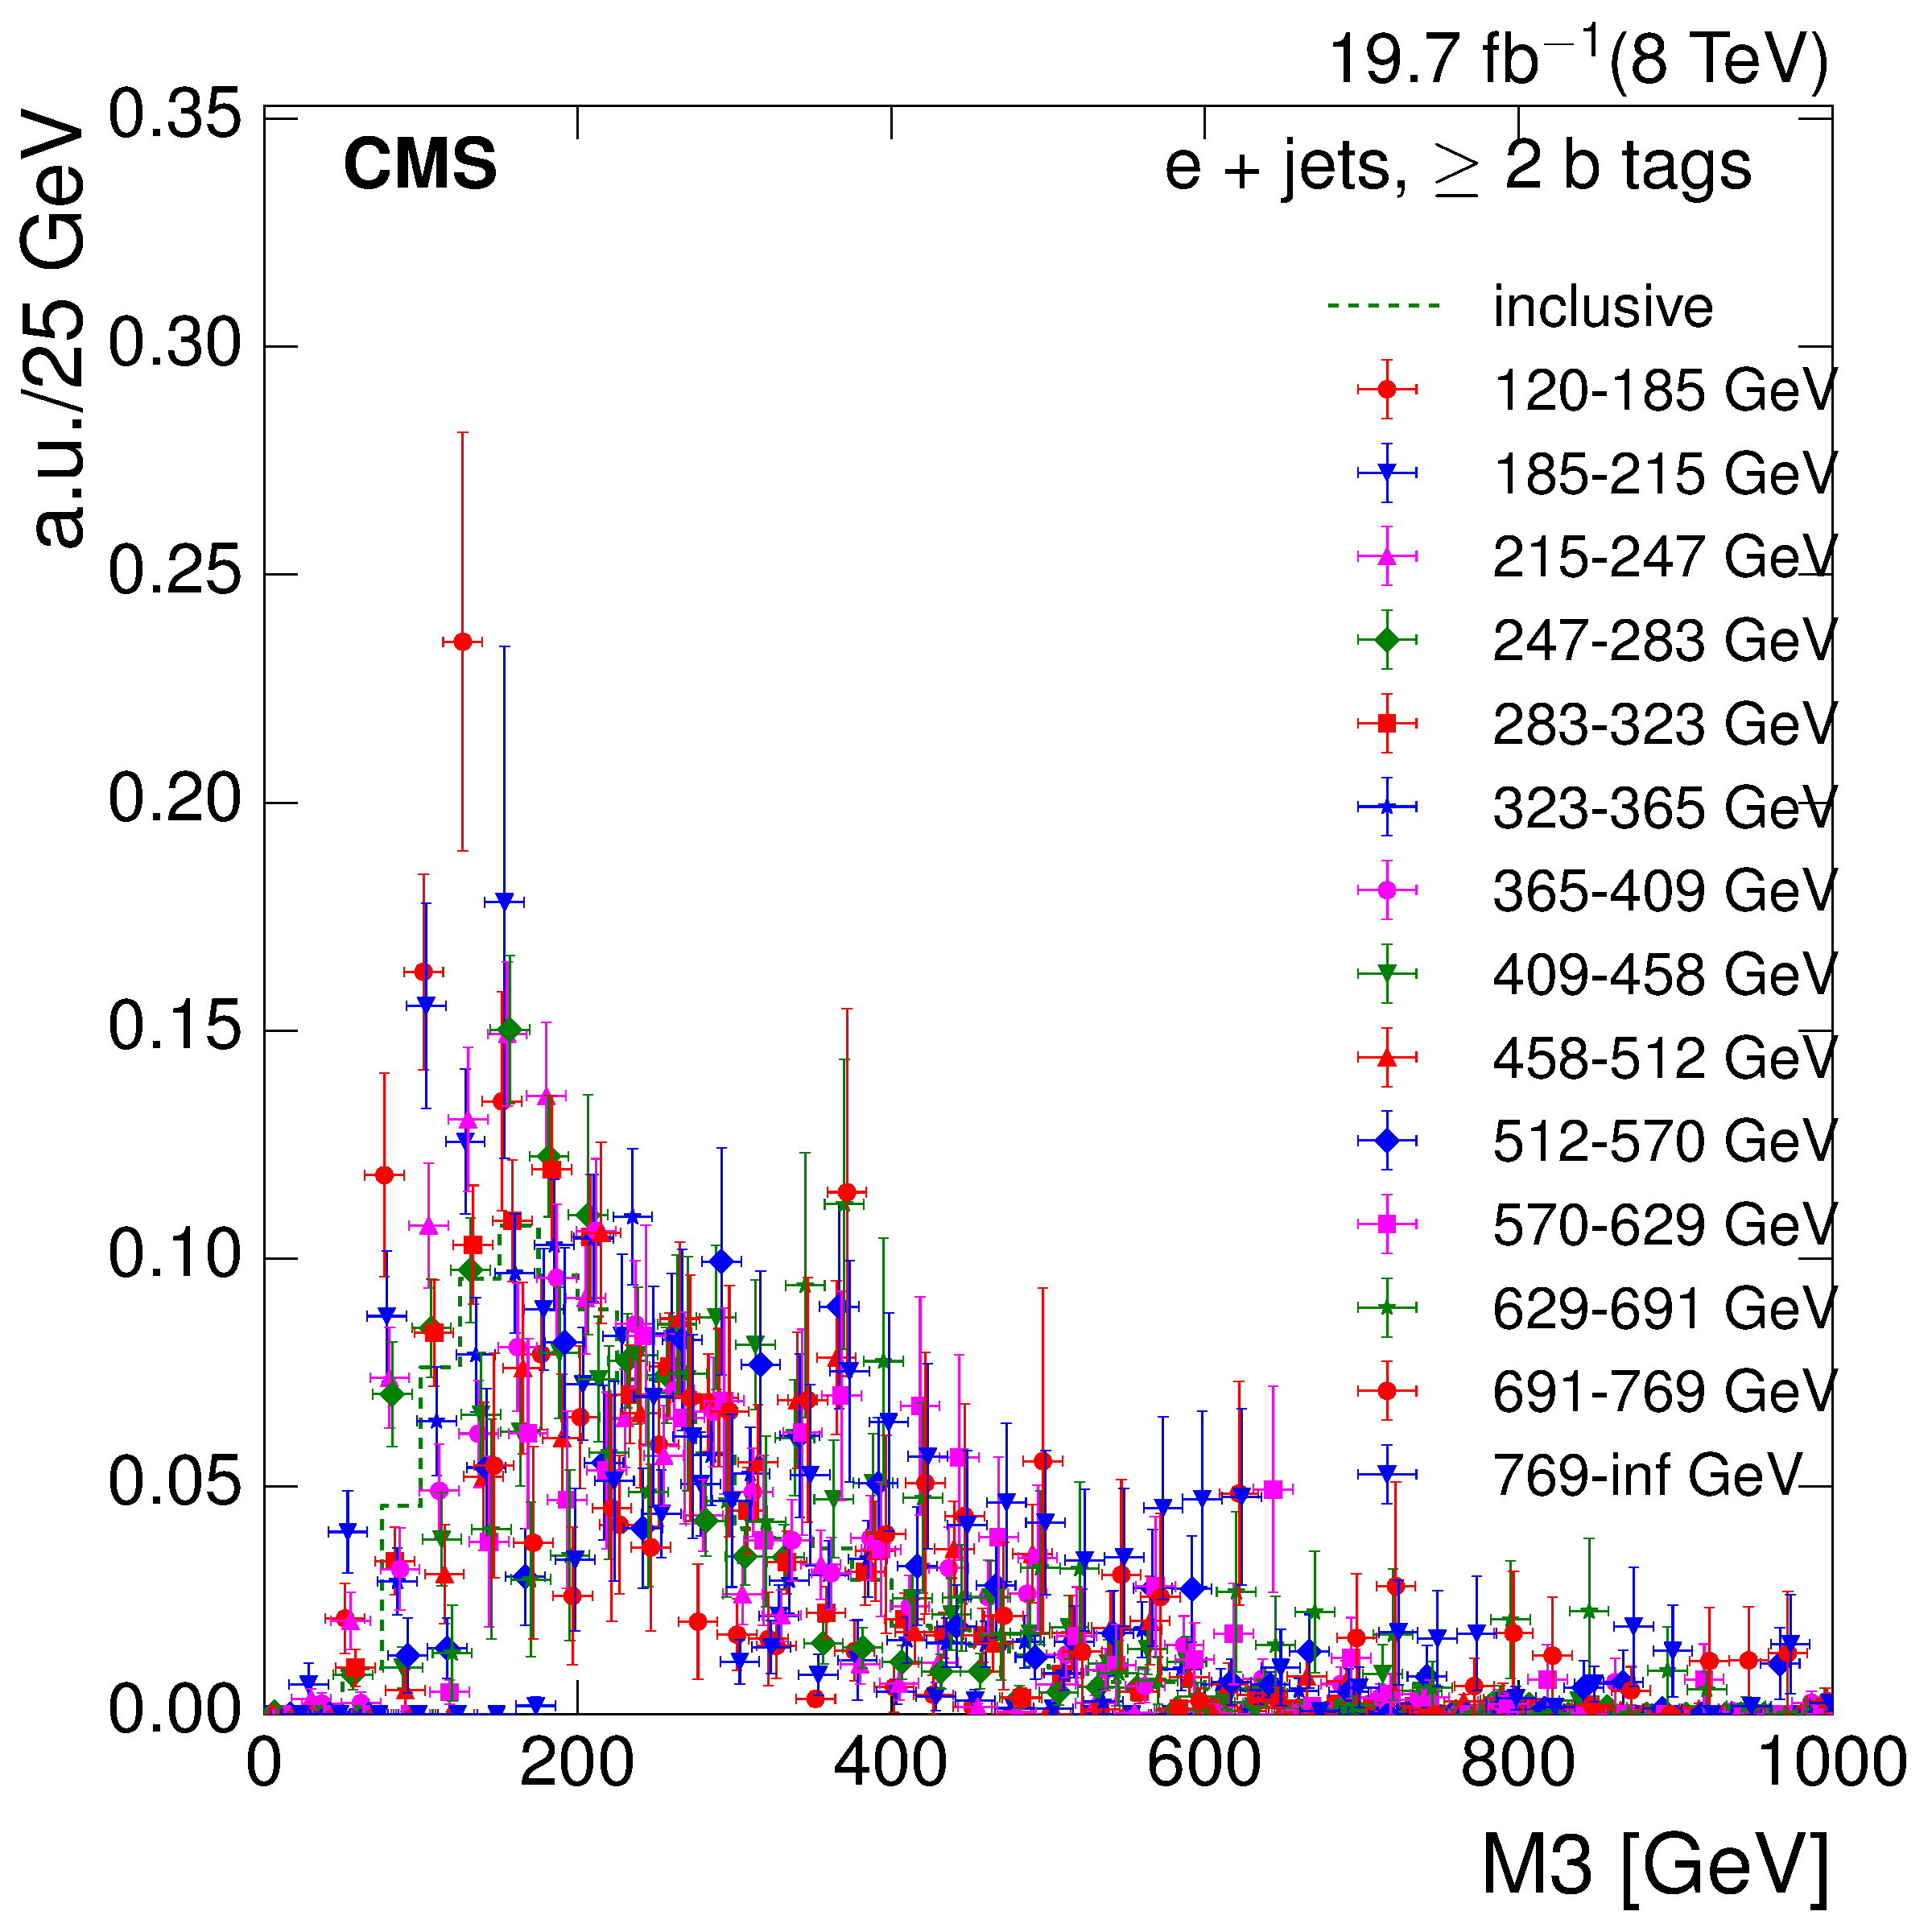
\includegraphics[width=0.48\textwidth]{Chapters/07_08_09_Analysis/Images/8TeV/fit_variables/electron/HT/M3/vjets/HT_M3_2orMoreBtags_VJets_template_comparison.pdf}\hfill
%      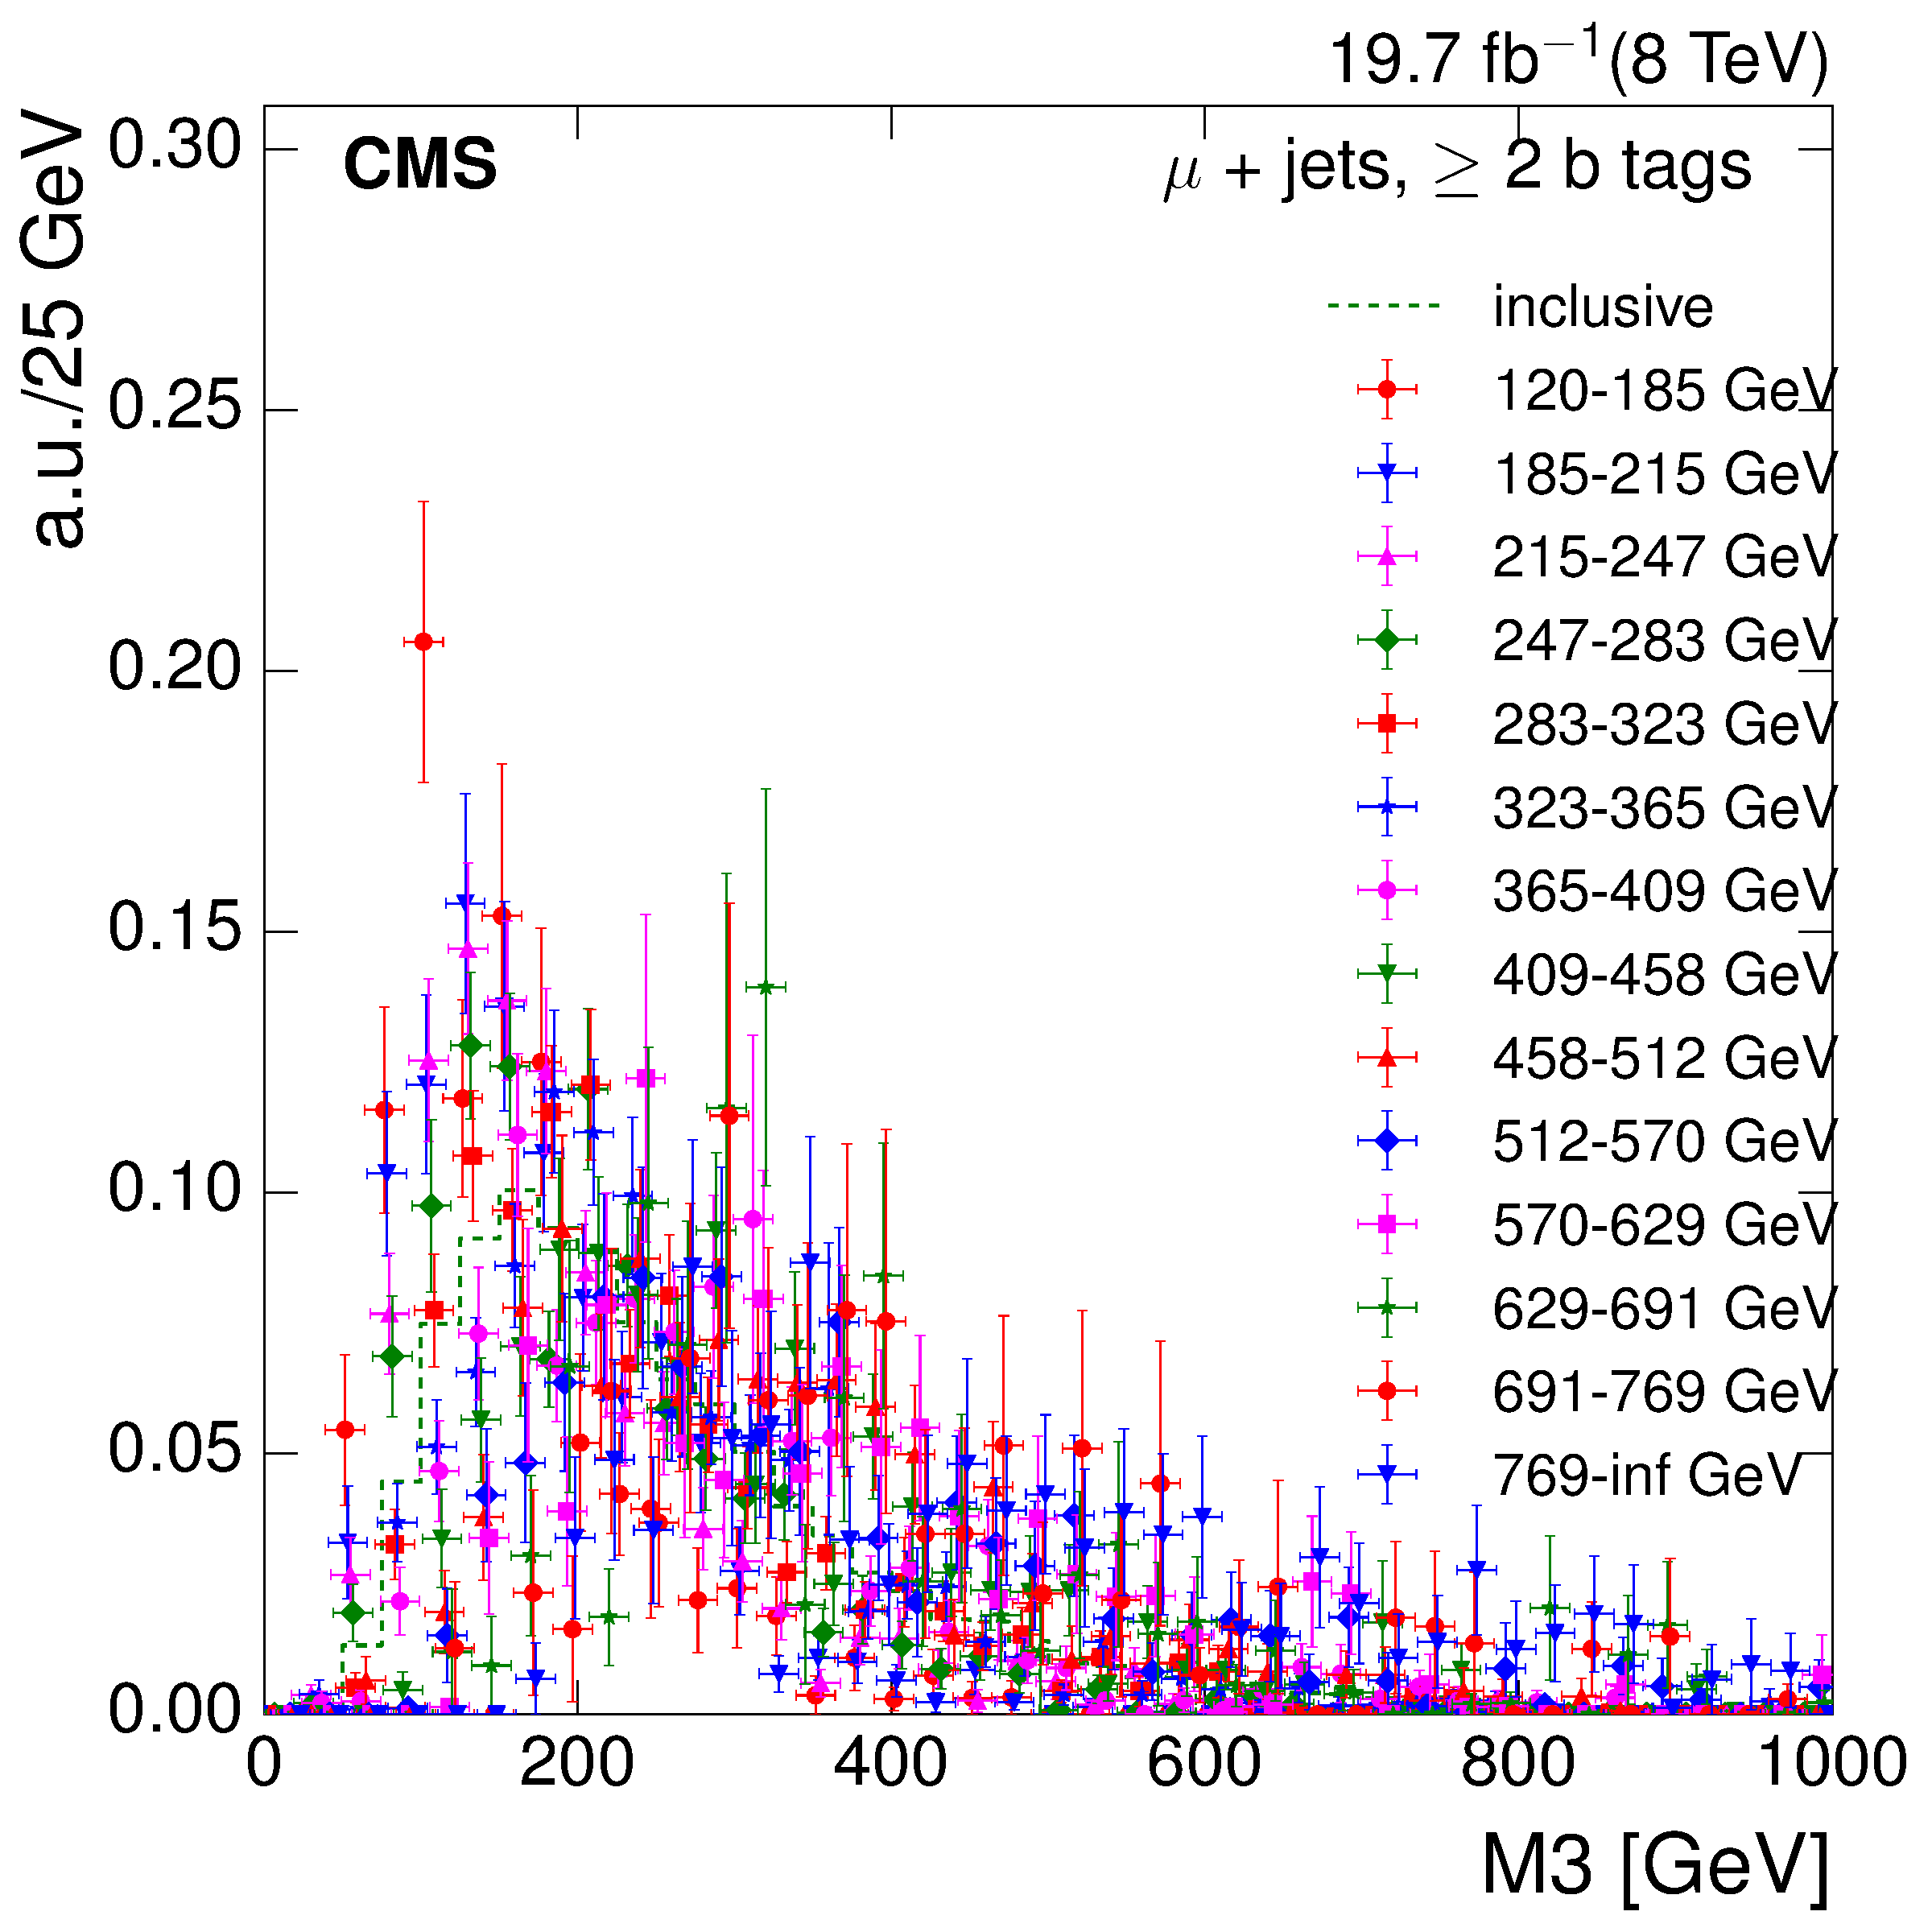
\includegraphics[width=0.48\textwidth]{Chapters/07_08_09_Analysis/Images/8TeV/fit_variables/muon/HT/M3/vjets/HT_M3_2orMoreBtags_VJets_template_comparison.pdf}\\
% 	 \caption[Normalised distributions of the V+jets templates for the three fit variables in \HT
% 	 bins at $\sqrt{s}=8\TeV$.]{Normalised distributions of the V+jets templates for the three fit variables
% 	 lepton \abseta (upper), $\alpha$ (middle) and M3 (lower) inclusive across all \HT bins and for individual
% 	 \HT bins at $\sqrt{s}=8\TeV$ in the electron+jets channel (left) and in the muon+jets channel (right).}
%      \label{fig:HT_fit_variable_vjets_comparisons_8TeV}
% \end{figure}
% 
% \begin{figure}[hbtp]
%     \centering
%      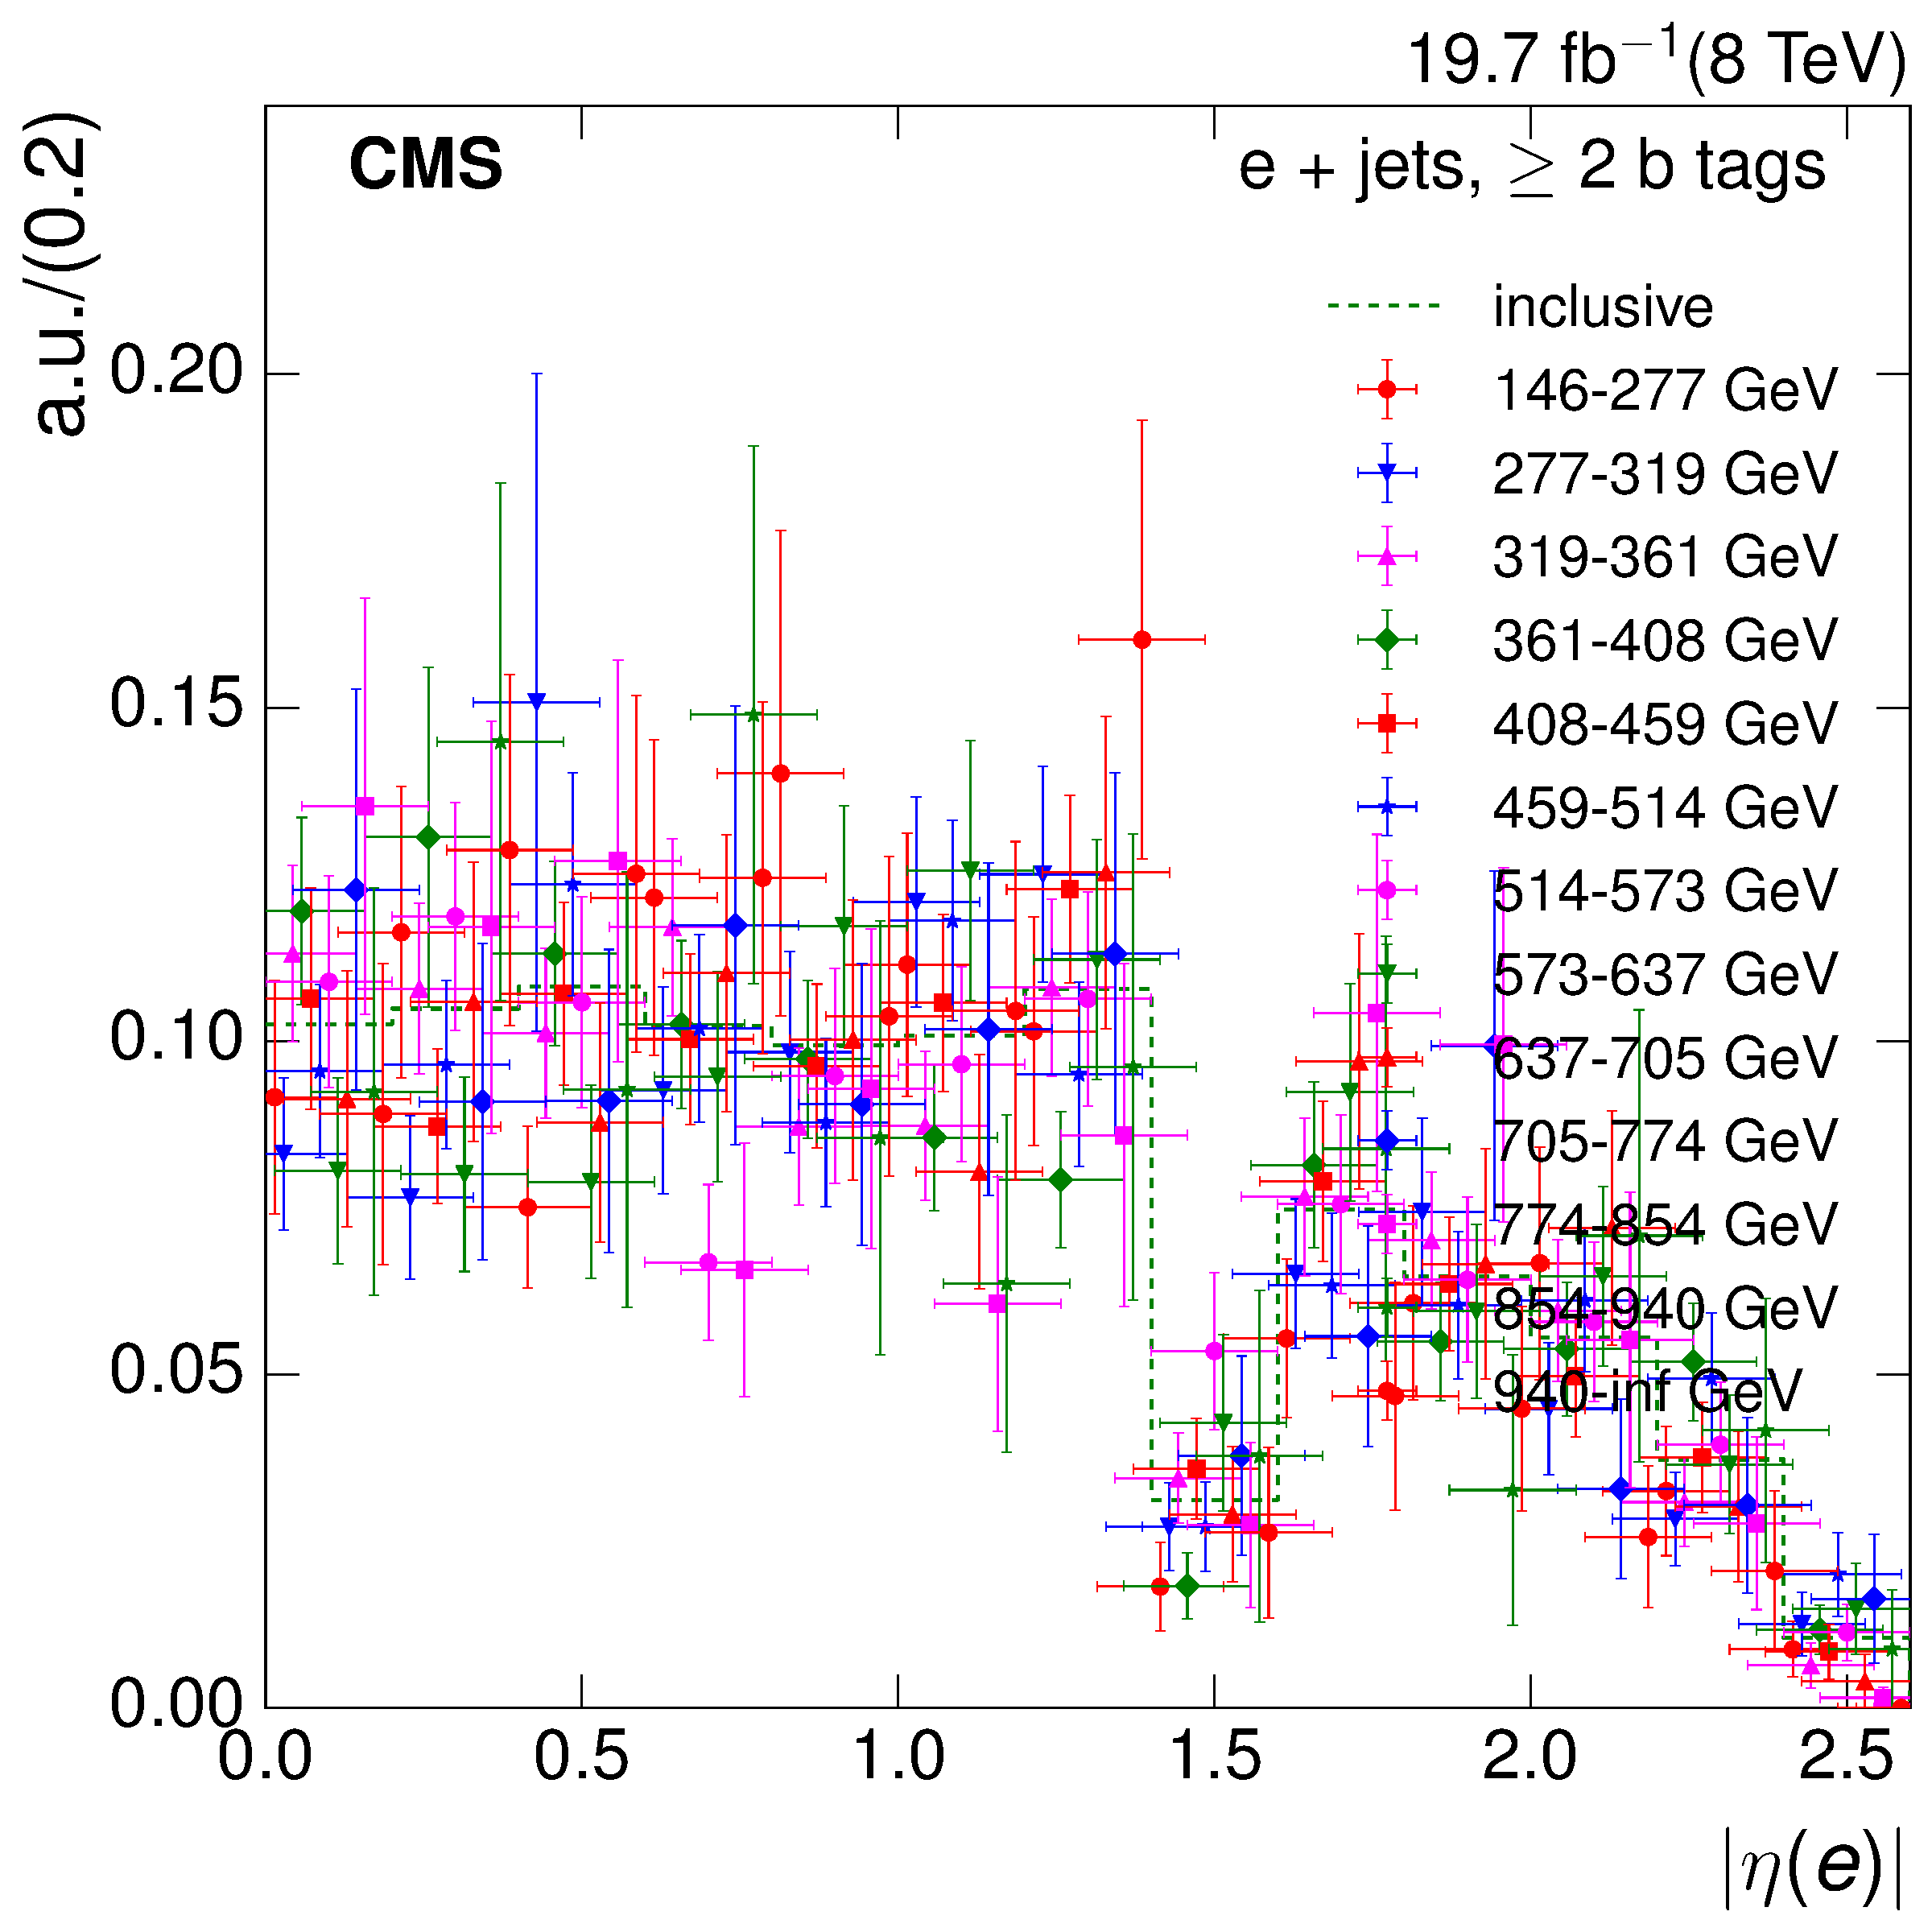
\includegraphics[width=0.48\textwidth]{Chapters/07_08_09_Analysis/Images/8TeV/fit_variables/electron/ST/electron_absolute_eta/vjets/ST_electron_absolute_eta_2orMoreBtags_VJets_template_comparison.pdf}\hfill
%      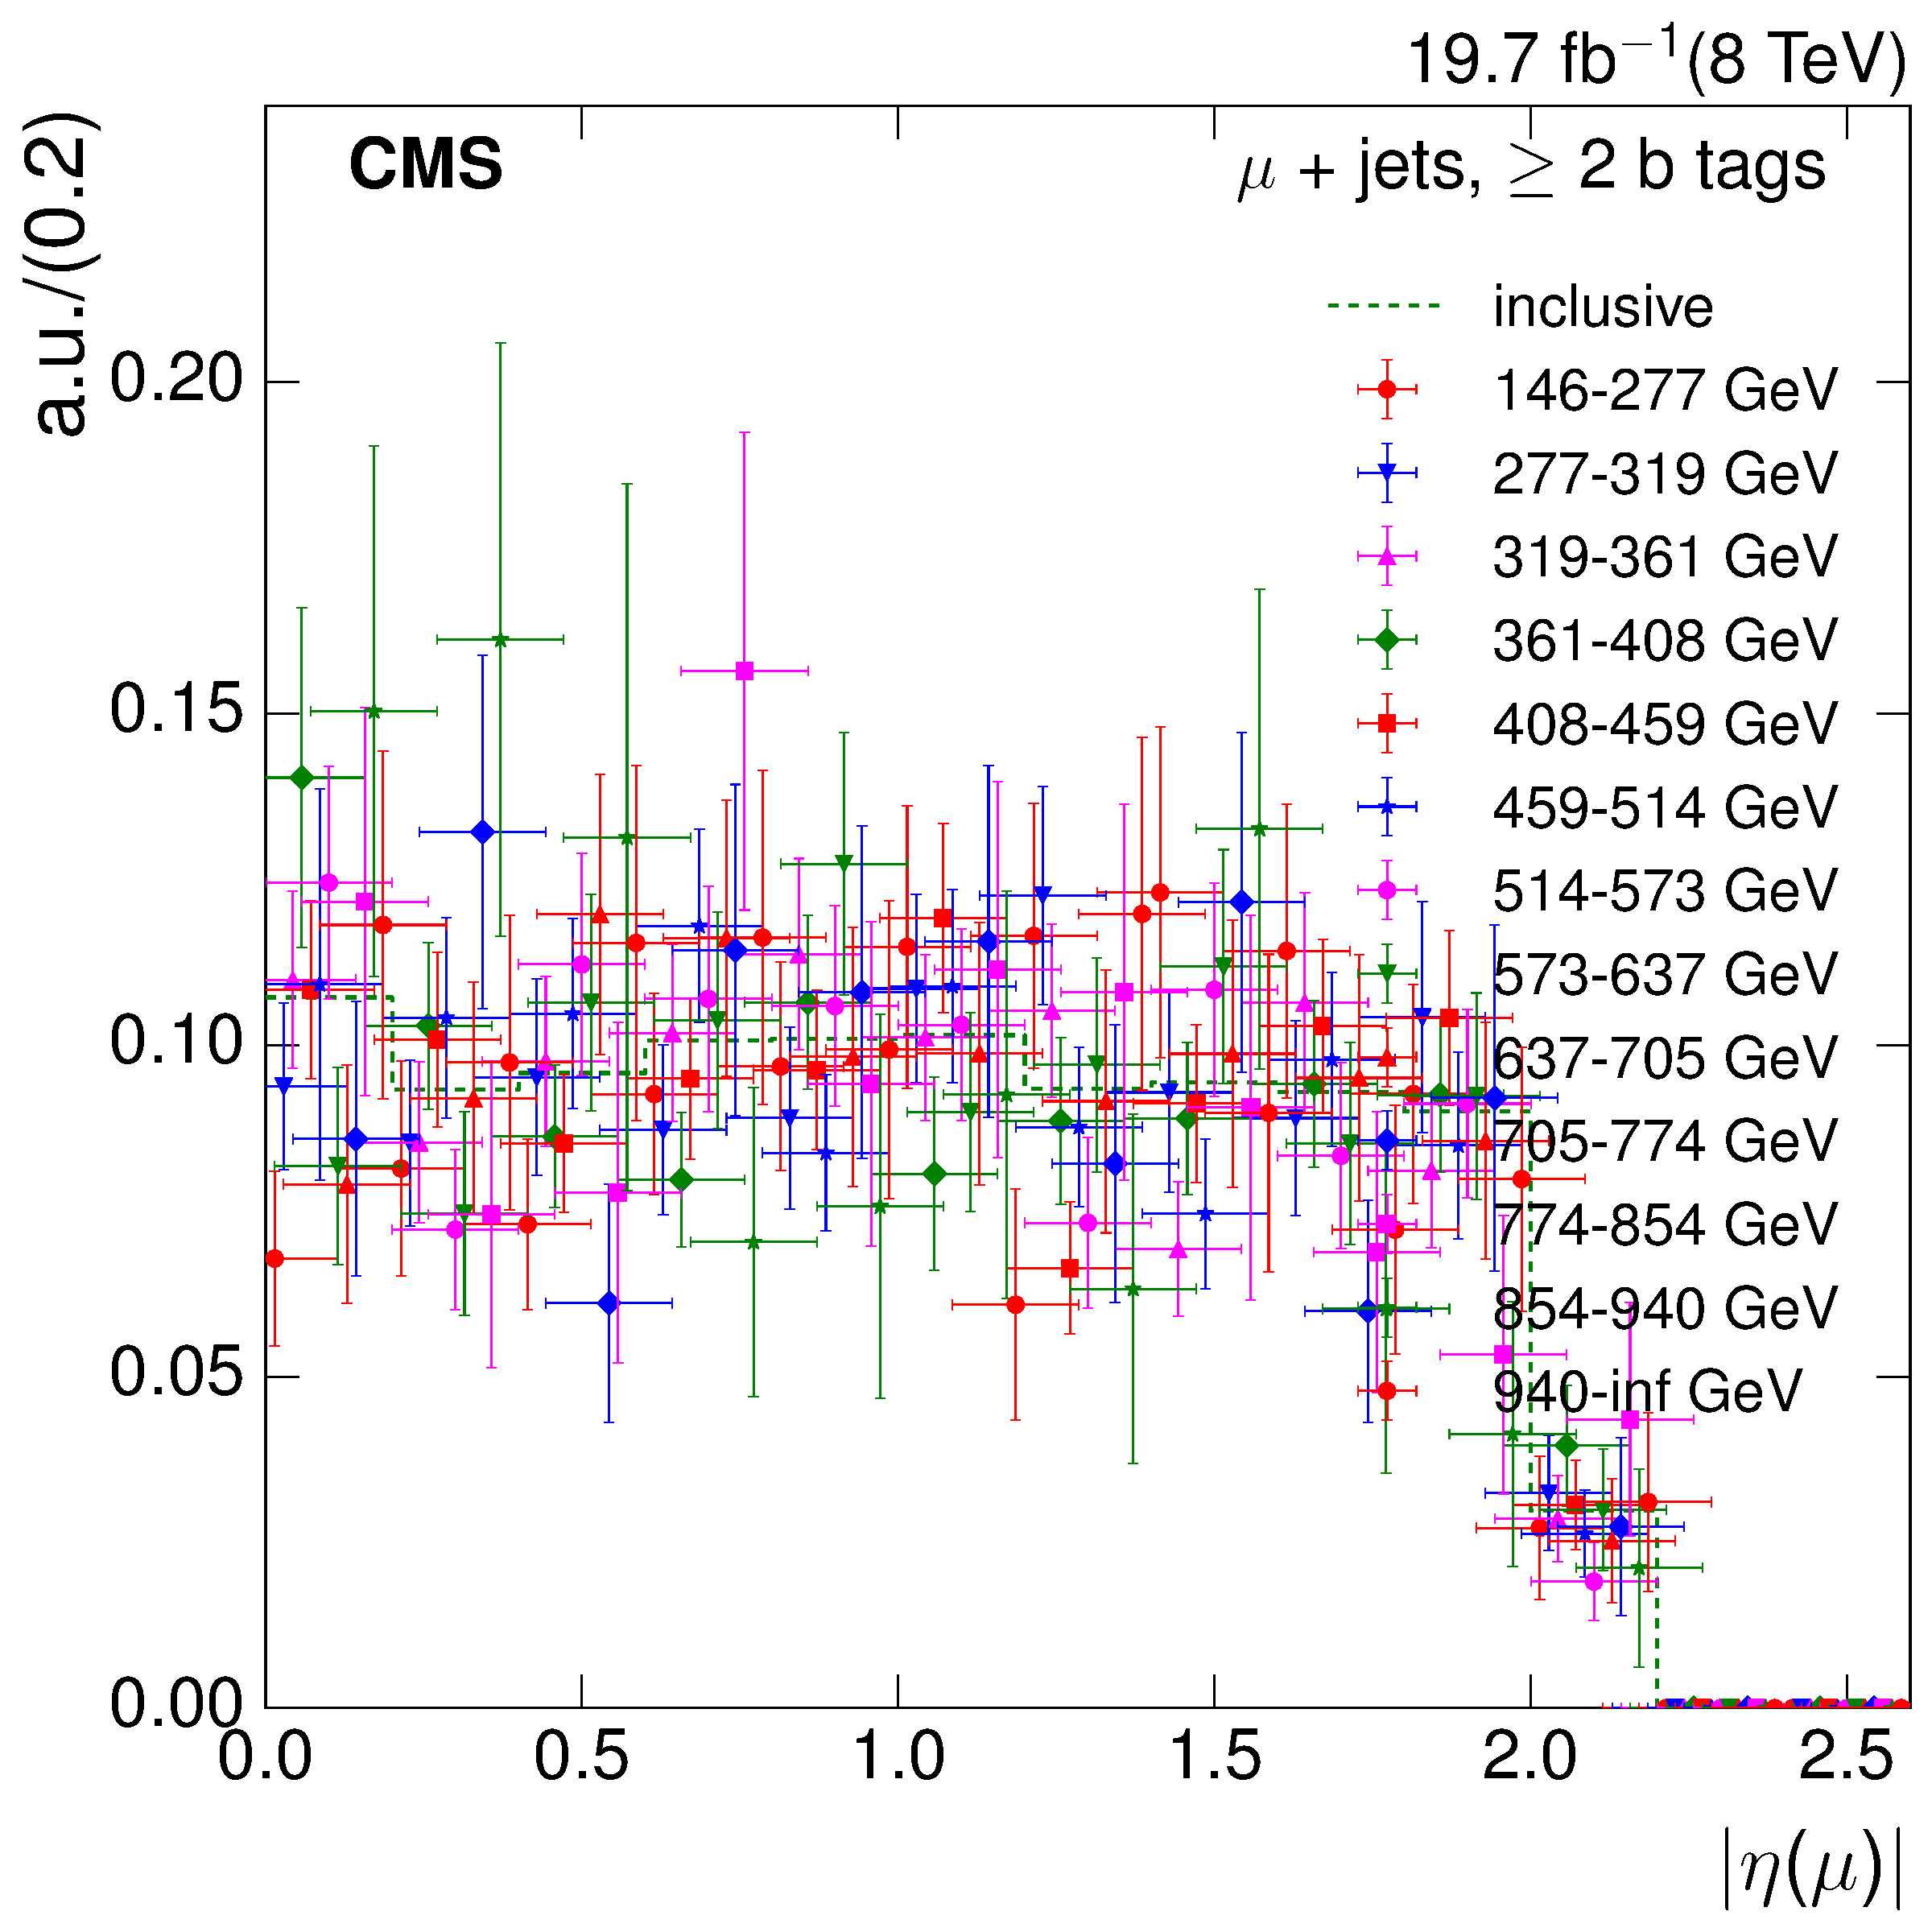
\includegraphics[width=0.48\textwidth]{Chapters/07_08_09_Analysis/Images/8TeV/fit_variables/muon/ST/muon_absolute_eta/vjets/ST_muon_absolute_eta_2orMoreBtags_VJets_template_comparison.pdf}\\
%      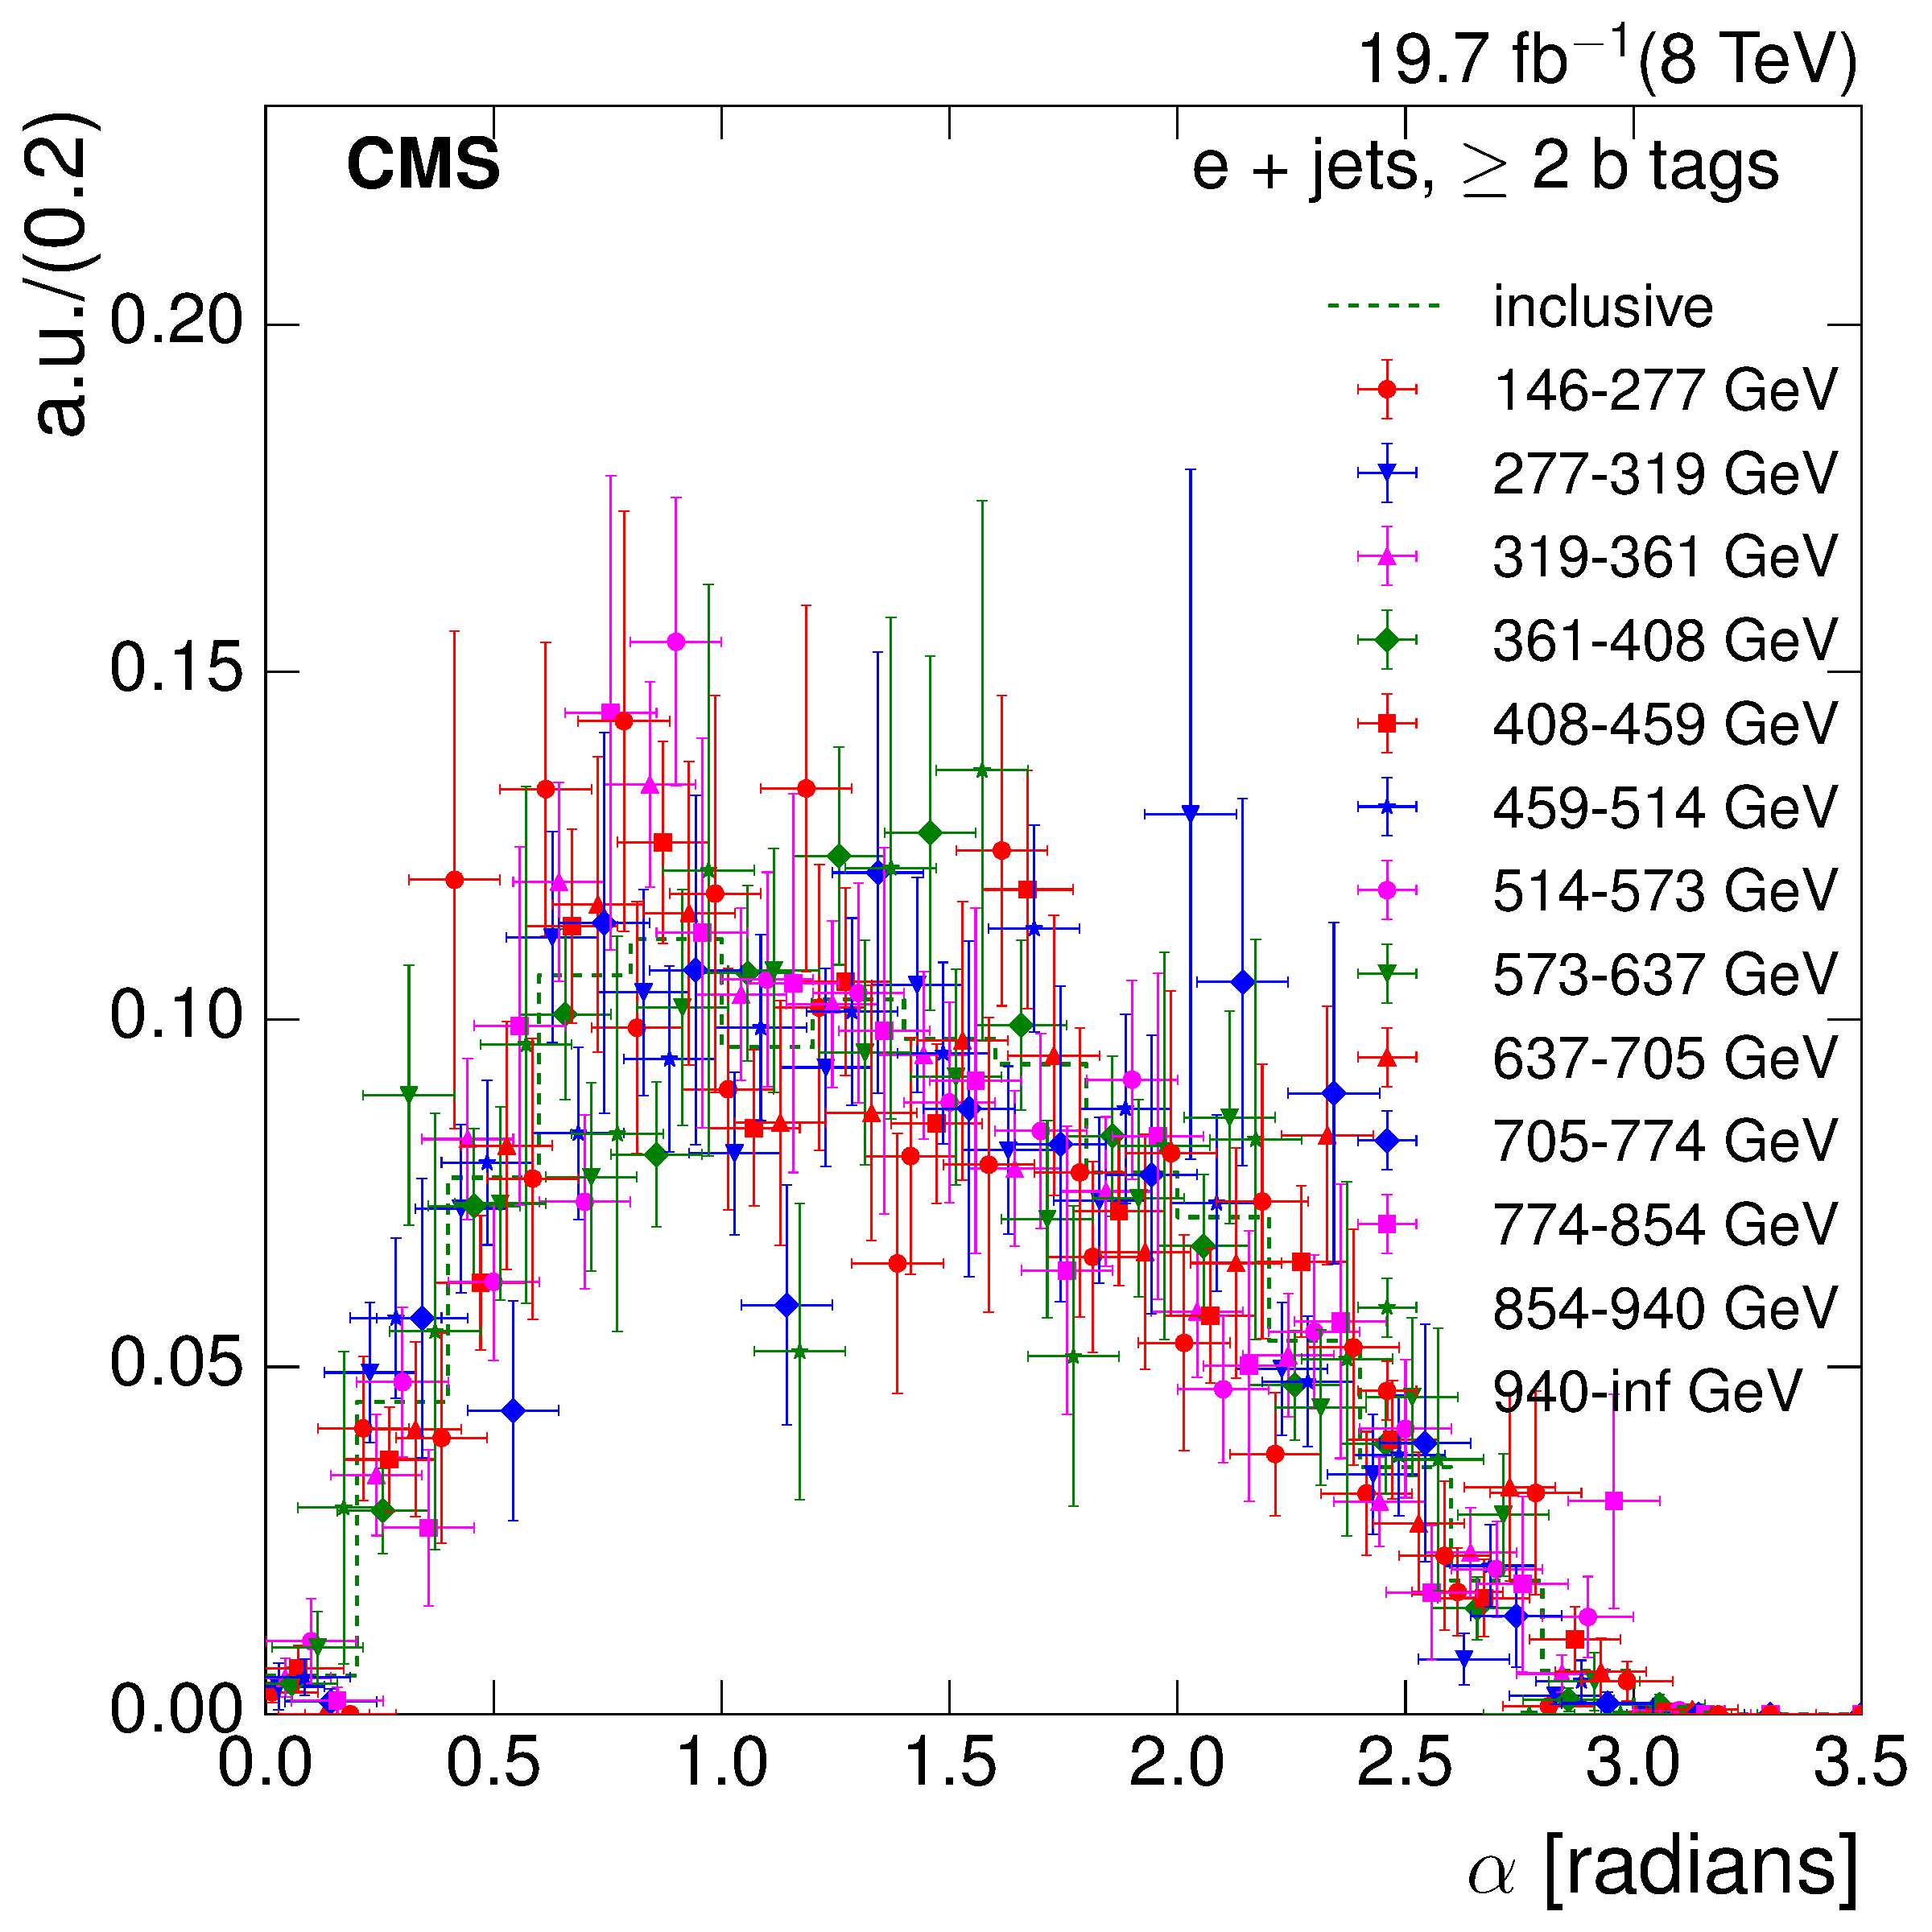
\includegraphics[width=0.48\textwidth]{Chapters/07_08_09_Analysis/Images/8TeV/fit_variables/electron/ST/angle_bl/vjets/ST_angle_bl_2orMoreBtags_VJets_template_comparison.pdf}\hfill
%      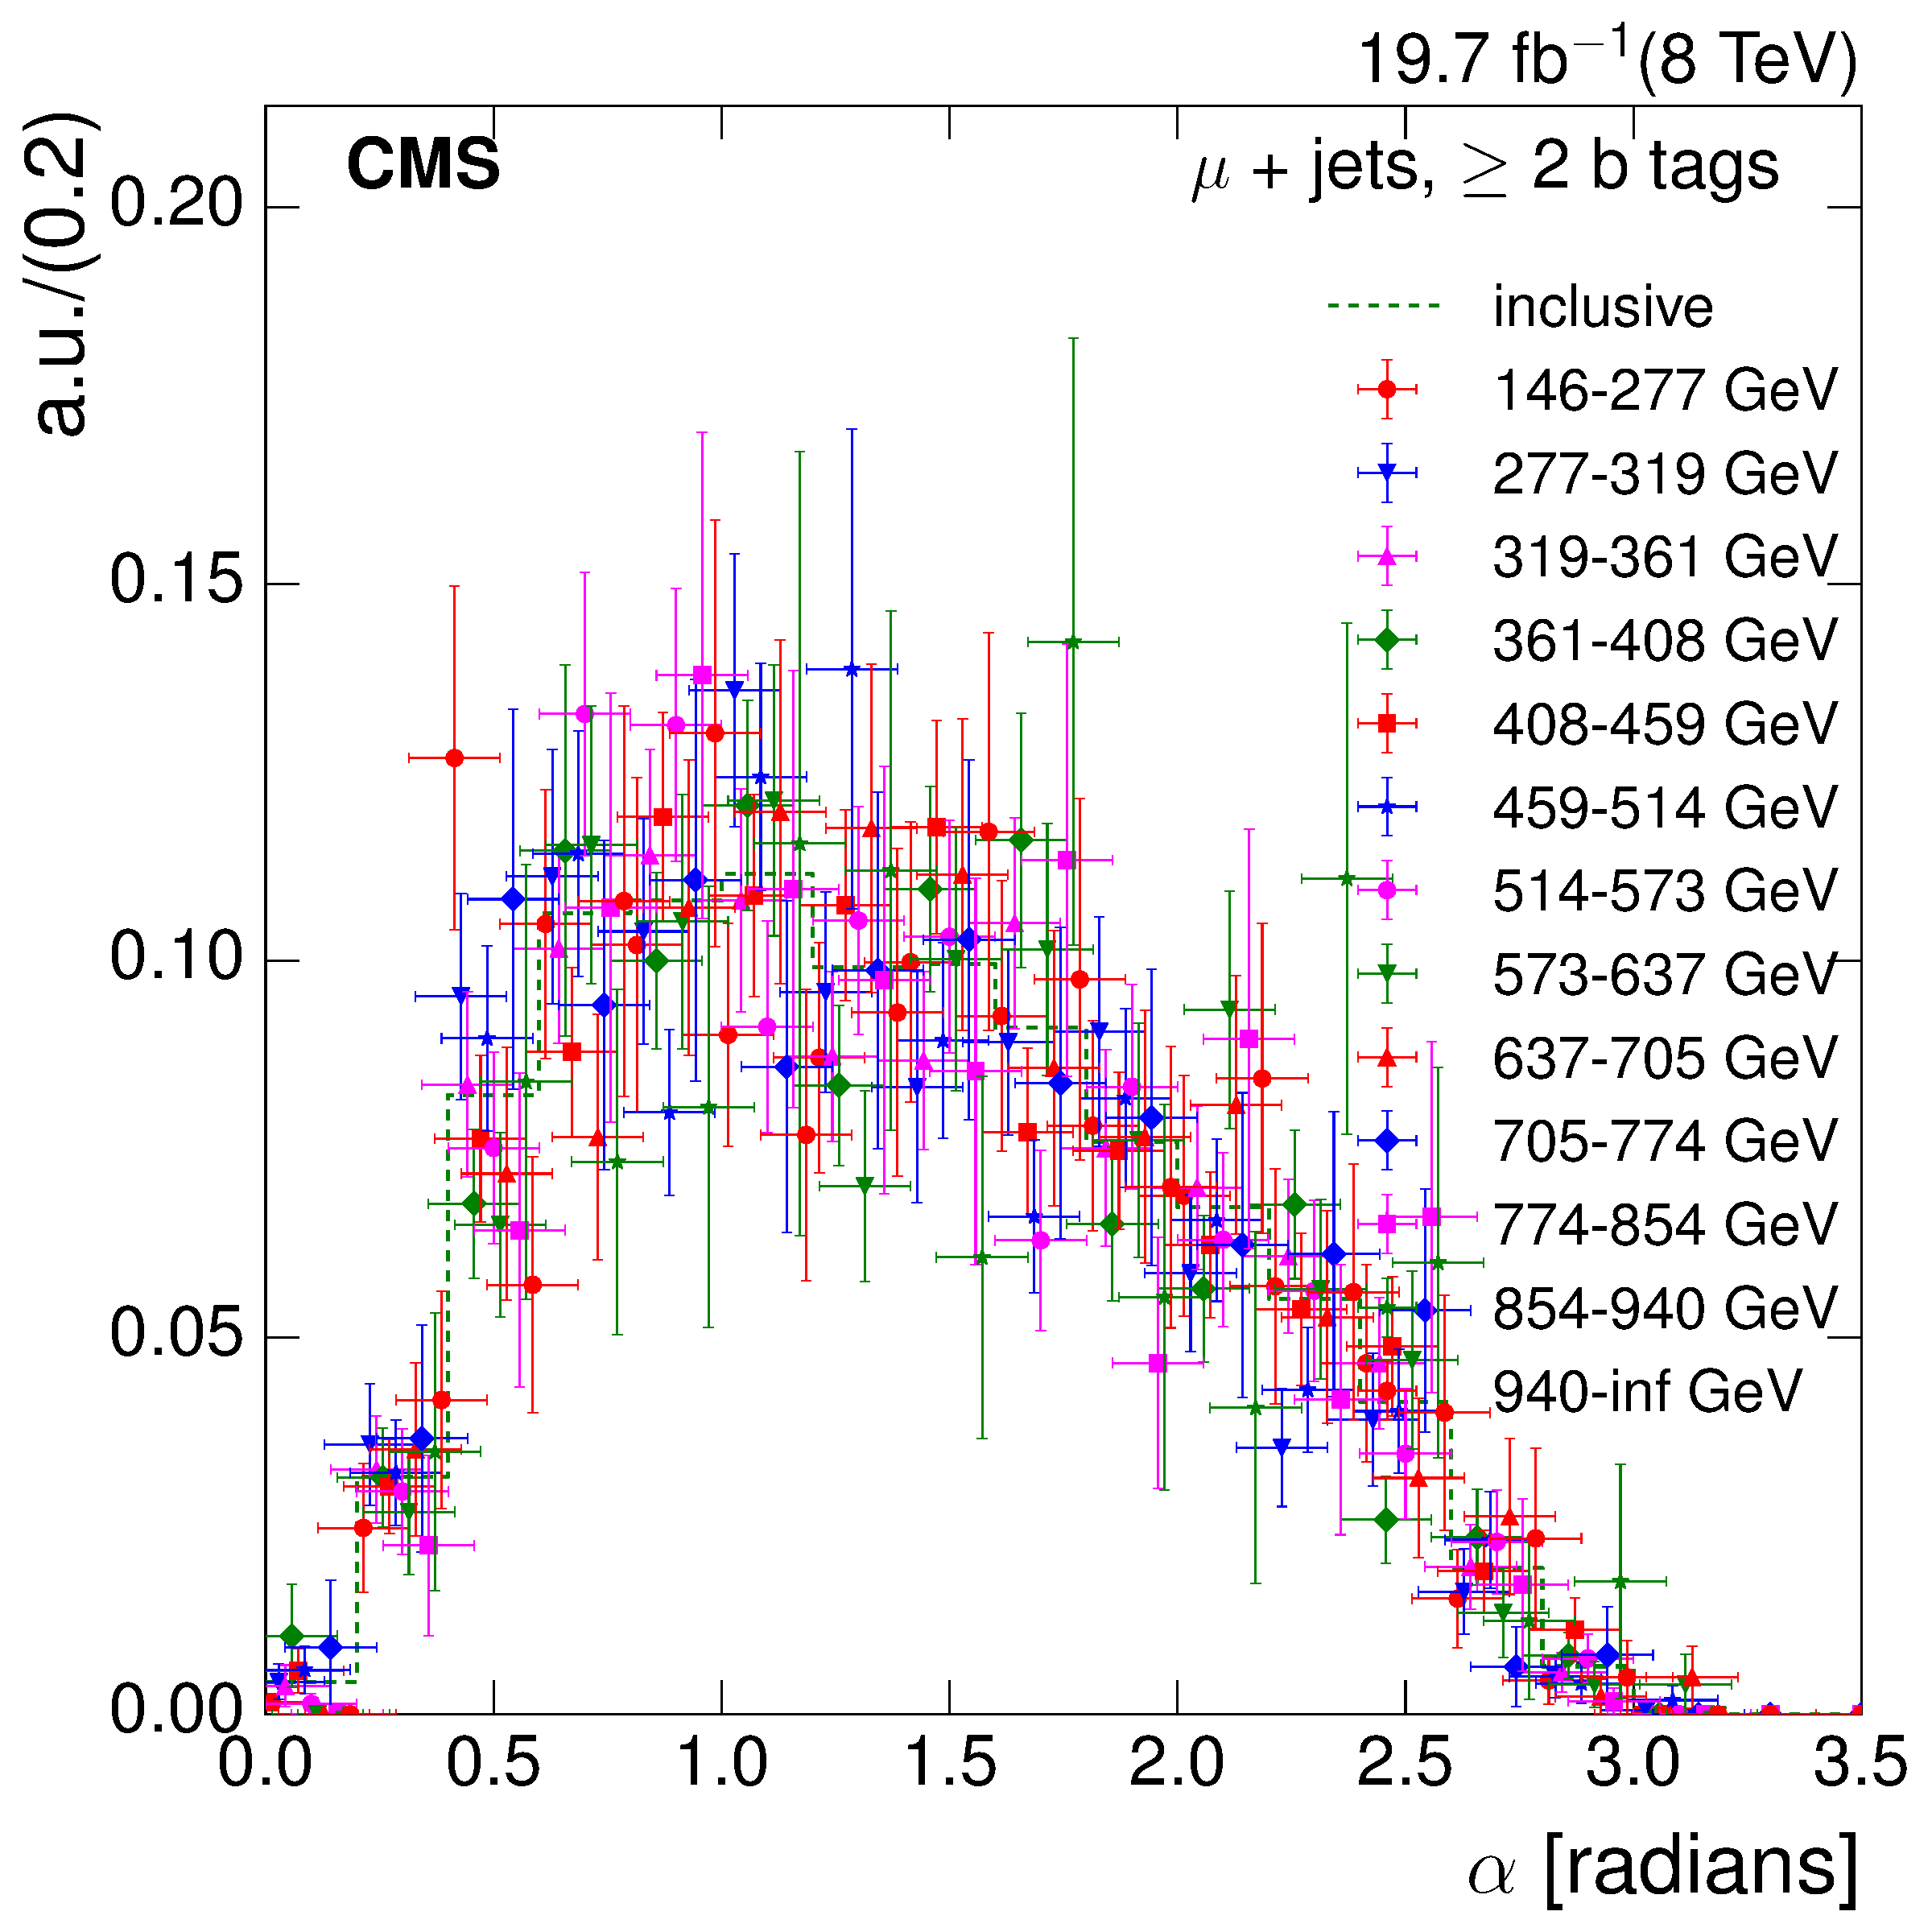
\includegraphics[width=0.48\textwidth]{Chapters/07_08_09_Analysis/Images/8TeV/fit_variables/muon/ST/angle_bl/vjets/ST_angle_bl_2orMoreBtags_VJets_template_comparison.pdf}\\
%      \includegraphics[width=0.48\textwidth]{Chapters/07_08_09_Analysis/Images/8TeV/fit_variables/electron/ST/M3/vjets/ST_M3_2orMoreBtags_VJets_template_comparison.pdf}\hfill
%      \includegraphics[width=0.48\textwidth]{Chapters/07_08_09_Analysis/Images/8TeV/fit_variables/muon/ST/M3/vjets/ST_M3_2orMoreBtags_VJets_template_comparison.pdf}\\
% 	 \caption[Normalised distributions of the V+jets templates for the three fit variables in \st
% 	 bins at $\sqrt{s}=8\TeV$.]{Normalised distributions of the V+jets templates for the three fit variables
% 	 lepton \abseta (upper), $\alpha$ (middle) and M3 (lower) inclusive across all \st bins and for individual
% 	 \st bins at $\sqrt{s}=8\TeV$ in the electron+jets channel (left) and in the muon+jets channel (right).}
%      \label{fig:ST_fit_variable_vjets_comparisons_8TeV}
% \end{figure}
% 
% \begin{figure}[hbtp]
%     \centering
%      \includegraphics[width=0.48\textwidth]{Chapters/07_08_09_Analysis/Images/8TeV/fit_variables/electron/MT/electron_absolute_eta/vjets/MT_electron_absolute_eta_2orMoreBtags_VJets_template_comparison.pdf}\hfill
%      \includegraphics[width=0.48\textwidth]{Chapters/07_08_09_Analysis/Images/8TeV/fit_variables/muon/MT/muon_absolute_eta/vjets/MT_muon_absolute_eta_2orMoreBtags_VJets_template_comparison.pdf}\\
%      \includegraphics[width=0.48\textwidth]{Chapters/07_08_09_Analysis/Images/8TeV/fit_variables/electron/MT/angle_bl/vjets/MT_angle_bl_2orMoreBtags_VJets_template_comparison.pdf}\hfill
%      \includegraphics[width=0.48\textwidth]{Chapters/07_08_09_Analysis/Images/8TeV/fit_variables/muon/MT/angle_bl/vjets/MT_angle_bl_2orMoreBtags_VJets_template_comparison.pdf}\\
%      \includegraphics[width=0.48\textwidth]{Chapters/07_08_09_Analysis/Images/8TeV/fit_variables/electron/MT/M3/vjets/MT_M3_2orMoreBtags_VJets_template_comparison.pdf}\hfill
%      \includegraphics[width=0.48\textwidth]{Chapters/07_08_09_Analysis/Images/8TeV/fit_variables/muon/MT/M3/vjets/MT_M3_2orMoreBtags_VJets_template_comparison.pdf}\\
% 	 \caption[Normalised distributions of the V+jets templates for the three fit variables in \mt
% 	 bins at $\sqrt{s}=8\TeV$.]{Normalised distributions of the V+jets templates for the three fit variables
% 	 lepton \abseta (upper), $\alpha$ (middle) and M3 (lower) inclusive across all \mt bins and for individual
% 	 \mt bins at $\sqrt{s}=8\TeV$ in the electron+jets channel (left) and in the muon+jets channel (right).}
%      \label{fig:MT_fit_variable_vjets_comparisons_8TeV}
% \end{figure}
% 
% \begin{figure}[hbtp]
%     \centering
%      \includegraphics[width=0.48\textwidth]{Chapters/07_08_09_Analysis/Images/8TeV/fit_variables/electron/WPT/electron_absolute_eta/vjets/WPT_electron_absolute_eta_2orMoreBtags_VJets_template_comparison.pdf}\hfill
%      \includegraphics[width=0.48\textwidth]{Chapters/07_08_09_Analysis/Images/8TeV/fit_variables/muon/WPT/muon_absolute_eta/vjets/WPT_muon_absolute_eta_2orMoreBtags_VJets_template_comparison.pdf}\\
%      \includegraphics[width=0.48\textwidth]{Chapters/07_08_09_Analysis/Images/8TeV/fit_variables/electron/WPT/angle_bl/vjets/WPT_angle_bl_2orMoreBtags_VJets_template_comparison.pdf}\hfill
%      \includegraphics[width=0.48\textwidth]{Chapters/07_08_09_Analysis/Images/8TeV/fit_variables/muon/WPT/angle_bl/vjets/WPT_angle_bl_2orMoreBtags_VJets_template_comparison.pdf}\\
%      \includegraphics[width=0.48\textwidth]{Chapters/07_08_09_Analysis/Images/8TeV/fit_variables/electron/WPT/M3/vjets/WPT_M3_2orMoreBtags_VJets_template_comparison.pdf}\hfill
%      \includegraphics[width=0.48\textwidth]{Chapters/07_08_09_Analysis/Images/8TeV/fit_variables/muon/WPT/M3/vjets/WPT_M3_2orMoreBtags_VJets_template_comparison.pdf}\\
% 	 \caption[Normalised distributions of the V+jets templates for the three fit variables in \wpt
% 	 bins at $\sqrt{s}=8\TeV$]{Normalised distributions of the V+jets templates for the three fit variables
% 	 lepton \abseta (upper), $\alpha$ (middle) and M3 (lower) inclusive across all \wpt bins and for individual
% 	 \wpt bins at $\sqrt{s}=8\TeV$ in the electron+jets channel (left) and in the muon+jets channel (right).}
%      \label{fig:WPT_fit_variable_vjets_comparisons_8TeV}
% \end{figure}


\clearpage
\section{Fit Results Tables}
\label{as:fit_results_tables}

%% ============================================================
% Fit results for MET variable, electron channel, met type patType1CorrectedPFMet 
%% ============================================================
\begin{table}[htbp]
\centering
\caption{Fit results for the \MET variable
at a centre-of-mass energy of 7 TeV (electron channel).}
\label{tab:MET_fit_results_7TeV_electron}
\resizebox{\columnwidth}{!} {
\begin{tabular}{lrrrrrrr}
\hline
Process & 0--27~\GeV & 27--52~\GeV & 52--87~\GeV & 87--130~\GeV & 130--172~\GeV & $\geq 172$~\GeV& Total \\
\hline
$\mathrm{t}\bar{\mathrm{t}}$ in & 2526.0 $\pm$ 41.1 & 4512.2 $\pm$ 54.0 & 4013.3 $\pm$ 55.7 & 1725.2 $\pm$ 33.3 & 518.4 $\pm$ 18.5 & 287.8 $\pm$ 12.2 & 13582.9 $\pm$ 214.8 \\
$\mathrm{t}\bar{\mathrm{t}}$ fit & 2444.9 $\pm$ 90.2 & 3902.5 $\pm$ 159.0 & 3610.7 $\pm$ 148.6 & 1447.3 $\pm$ 83.5 & 366.1 $\pm$ 34.8 & 202.0 $\pm$ 24.1 & 11973.6 $\pm$ 540.2 \\
\hline
Single Top in & 82.4 $\pm$ 6.7 & 143.2 $\pm$ 8.9 & 120.1 $\pm$ 7.7 & 50.5 $\pm$ 4.9 & 19.6 $\pm$ 3.1 & 12.0 $\pm$ 2.1 & 427.8 $\pm$ 33.4 \\
Single Top fit & 0.0 $\pm$ 381.7 & 341.0 $\pm$ 197.4 & 212.6 $\pm$ 181.9 & 82.4 $\pm$ 88.3 & 59.3 $\pm$ 33.1 & 57.1 $\pm$ 21.2 & 752.3 $\pm$ 903.6 \\
\hline
W/Z + jets in & 121.0 $\pm$ 8.7 & 138.7 $\pm$ 9.9 & 82.9 $\pm$ 5.9 & 30.9 $\pm$ 2.2 & 12.8 $\pm$ 0.9 & 9.4 $\pm$ 0.7 & 395.7 $\pm$ 28.3 \\
W/Z + jets fit & 403.7 $\pm$ 125.3 & 342.4 $\pm$ 110.5 & 160.7 $\pm$ 105.0 & 109.3 $\pm$ 58.0 & 0.0 $\pm$ 40.5 & 4.9 $\pm$ 13.6 & 1021.0 $\pm$ 452.9 \\
\hline
QCD in & 323.3 $\pm$ 15.0 & 242.9 $\pm$ 11.3 & 9.0 $\pm$ 0.4 & 1.3 $\pm$ 0.1 & 1.0 $\pm$ 0.0 & 1.0 $\pm$ 0.0 & 578.5 $\pm$ 26.8 \\
QCD fit & 31.4 $\pm$ 56.6 & 0.0 $\pm$ 25.7 & 0.0 $\pm$ 88.1 & 0.0 $\pm$ 15.5 & 13.6 $\pm$ 11.0 & 0.0 $\pm$ 82.7 & 45.1 $\pm$ 279.6 \\
\hline
Sum MC in & 3052.7 $\pm$ 71.5 & 5037.0 $\pm$ 84.1 & 4225.3 $\pm$ 69.7 & 1807.8 $\pm$ 40.5 & 551.8 $\pm$ 22.6 & 310.3 $\pm$ 15.0& 14984.9 $\pm$ 303.4 \\
Sum MC fit & 2880.0 $\pm$ 653.8 & 4586.0 $\pm$ 492.5 & 3984.0 $\pm$ 523.6 & 1639.0 $\pm$ 245.3 & 439.0 $\pm$ 119.5 & 264.0 $\pm$ 141.6 & 13792.0 $\pm$ 2176.3 \\
\hline
Data & 2880.0 $\pm$ 180.1 & 4586.0 $\pm$ 226.1 & 3984.0 $\pm$ 207.8 & 1639.0 $\pm$ 132.0 & 439.0 $\pm$ 66.7 & 264.0 $\pm$ 49.6 & 13792.0 $\pm$ 862.2 \\
\hline
\end{tabular}
}
\end{table}

%% ============================================================
% Fit results for MET variable, muon channel, met type patType1CorrectedPFMet 
%% ============================================================
\begin{table}[htbp]
\centering
\caption{Fit results for the \MET variable
at a centre-of-mass energy of 7 TeV (muon channel).}
\label{tab:MET_fit_results_7TeV_muon}
\resizebox{\columnwidth}{!} {
\begin{tabular}{lrrrrrrr}
\hline
Process & 0--27~\GeV & 27--52~\GeV & 52--87~\GeV & 87--130~\GeV & 130--172~\GeV & $\geq 172$~\GeV& Total \\
\hline
$\mathrm{t}\bar{\mathrm{t}}$ in & 2697.6 $\pm$ 41.5 & 4877.4 $\pm$ 57.9 & 4542.1 $\pm$ 52.0 & 1983.5 $\pm$ 34.2 & 594.9 $\pm$ 18.8 & 320.7 $\pm$ 13.0 & 15016.1 $\pm$ 217.4 \\
$\mathrm{t}\bar{\mathrm{t}}$ fit & 2026.2 $\pm$ 122.4 & 3800.8 $\pm$ 157.6 & 3729.3 $\pm$ 145.1 & 1475.9 $\pm$ 85.8 & 413.7 $\pm$ 39.0 & 200.7 $\pm$ 24.9 & 11646.6 $\pm$ 574.9 \\
\hline
Single Top in & 88.4 $\pm$ 6.7 & 150.6 $\pm$ 8.4 & 138.4 $\pm$ 8.4 & 57.6 $\pm$ 5.1 & 20.1 $\pm$ 3.0 & 13.9 $\pm$ 2.3 & 468.9 $\pm$ 33.9 \\
Single Top fit & 269.5 $\pm$ 150.0 & 397.2 $\pm$ 203.6 & 200.9 $\pm$ 164.4 & 83.5 $\pm$ 88.4 & 21.4 $\pm$ 33.7 & 35.3 $\pm$ 24.2 & 1007.8 $\pm$ 664.1 \\
\hline
W/Z + jets in & 107.9 $\pm$ 6.4 & 144.1 $\pm$ 8.6 & 103.6 $\pm$ 6.2 & 39.0 $\pm$ 2.3 & 11.5 $\pm$ 0.7 & 10.5 $\pm$ 0.6 & 416.5 $\pm$ 24.8 \\
W/Z + jets fit & 178.6 $\pm$ 119.9 & 198.1 $\pm$ 116.8 & 28.8 $\pm$ 101.6 & 43.6 $\pm$ 62.1 & 0.0 $\pm$ 35.8 & 9.0 $\pm$ 15.9 & 458.0 $\pm$ 452.1 \\
\hline
QCD in & 122.6 $\pm$ 5.1 & 22.6 $\pm$ 0.9 & 34.9 $\pm$ 1.5 & 0.1 $\pm$ 0.0 & 0.1 $\pm$ 0.0 & 0.1 $\pm$ 0.0 & 180.4 $\pm$ 7.5 \\
QCD fit & 4.7 $\pm$ 335.7 & 0.0 $\pm$ 370.4 & 0.0 $\pm$ 714.2 & 0.0 $\pm$ 253.2 & 10.9 $\pm$ 20.4 & 0.0 $\pm$ 18.8 & 15.6 $\pm$ 1712.7 \\
\hline
Sum MC in & 3016.5 $\pm$ 59.8 & 5194.7 $\pm$ 75.9 & 4819.1 $\pm$ 68.1 & 2080.2 $\pm$ 41.6 & 626.5 $\pm$ 22.4 & 345.1 $\pm$ 15.9& 16082.0 $\pm$ 283.7 \\
Sum MC fit & 2479.0 $\pm$ 727.9 & 4396.1 $\pm$ 848.5 & 3959.0 $\pm$ 1125.3 & 1603.0 $\pm$ 489.5 & 446.0 $\pm$ 128.9 & 245.0 $\pm$ 83.8 & 13128.1 $\pm$ 3403.9 \\
\hline
Data & 2479.0 $\pm$ 159.2 & 4396.0 $\pm$ 211.6 & 3959.0 $\pm$ 200.7 & 1603.0 $\pm$ 126.7 & 446.0 $\pm$ 65.9 & 245.0 $\pm$ 46.9 & 13128.0 $\pm$ 811.0 \\
\hline
\end{tabular}
}
\end{table}


\begin{landscape}
%% ============================================================
% Fit results for HT variable, electron channel, met type patType1CorrectedPFMet 
%% ============================================================
\begin{table}[htbp]
\centering
\caption{Fit results for the \HT variable
at a centre-of-mass energy of 7 TeV (electron channel).}
\label{tab:HT_fit_results_7TeV_electron}
\resizebox{\columnwidth}{!} {
\begin{tabular}{lrrrrrrrrrrrrrrr}
\hline
Process & 120--185~\GeV & 185--215~\GeV & 215--247~\GeV & 247--283~\GeV & 283--323~\GeV & 323--365~\GeV & 365--409~\GeV & 409--458~\GeV & 458--512~\GeV & 512--570~\GeV & 570--629~\GeV & 629--691~\GeV & 691--769~\GeV & $\geq 769$~\GeV& Total \\
\hline
$\mathrm{t}\bar{\mathrm{t}}$ in & 220.2 $\pm$ 11.4 & 769.6 $\pm$ 24.0 & 1478.9 $\pm$ 29.9 & 2001.7 $\pm$ 40.5 & 2101.2 $\pm$ 37.0 & 1827.6 $\pm$ 37.5 & 1451.0 $\pm$ 31.1 & 1176.7 $\pm$ 25.8 & 868.9 $\pm$ 23.5 & 602.5 $\pm$ 18.7 & 384.4 $\pm$ 14.7 & 257.2 $\pm$ 11.9 & 193.0 $\pm$ 10.5 & 249.9 $\pm$ 12.1 & 13582.9 $\pm$ 328.7 \\
$\mathrm{t}\bar{\mathrm{t}}$ fit & 197.0 $\pm$ 42.8 & 705.9 $\pm$ 72.2 & 1399.3 $\pm$ 91.5 & 1998.6 $\pm$ 110.9 & 1782.1 $\pm$ 89.0 & 1533.8 $\pm$ 71.0 & 1235.2 $\pm$ 66.6 & 934.0 $\pm$ 67.5 & 671.5 $\pm$ 49.7 & 533.4 $\pm$ 47.5 & 342.1 $\pm$ 34.4 & 200.0 $\pm$ 23.6 & 152.7 $\pm$ 20.1 & 188.2 $\pm$ 29.3 & 11873.8 $\pm$ 816.0 \\
\hline
Single Top in & 12.9 $\pm$ 2.5 & 32.2 $\pm$ 4.2 & 49.4 $\pm$ 5.0 & 59.5 $\pm$ 5.7 & 64.1 $\pm$ 5.9 & 53.3 $\pm$ 5.4 & 41.4 $\pm$ 4.6 & 33.6 $\pm$ 4.0 & 27.2 $\pm$ 3.6 & 18.2 $\pm$ 2.9 & 13.0 $\pm$ 2.6 & 7.7 $\pm$ 1.8 & 6.2 $\pm$ 1.7 & 9.2 $\pm$ 2.0 & 427.8 $\pm$ 51.7 \\
Single Top fit & 106.7 $\pm$ 45.0 & 120.0 $\pm$ 83.5 & 239.4 $\pm$ 101.8 & 13.1 $\pm$ 367.3 & 109.0 $\pm$ 121.5 & 48.5 $\pm$ 88.6 & 64.8 $\pm$ 68.8 & 134.0 $\pm$ 68.1 & 82.5 $\pm$ 46.9 & 31.4 $\pm$ 40.3 & 28.1 $\pm$ 30.7 & 7.2 $\pm$ 19.0 & 11.3 $\pm$ 18.0 & 45.6 $\pm$ 27.5 & 1041.6 $\pm$ 1127.1 \\
\hline
W/Z + jets in & 24.2 $\pm$ 1.7 & 34.0 $\pm$ 2.4 & 47.4 $\pm$ 3.4 & 47.3 $\pm$ 3.4 & 50.7 $\pm$ 3.6 & 43.5 $\pm$ 3.1 & 34.8 $\pm$ 2.5 & 31.8 $\pm$ 2.3 & 24.2 $\pm$ 1.7 & 22.0 $\pm$ 1.6 & 14.1 $\pm$ 1.0 & 6.1 $\pm$ 0.4 & 6.6 $\pm$ 0.5 & 9.1 $\pm$ 0.7 & 395.7 $\pm$ 28.3 \\
W/Z + jets fit & 0.0 $\pm$ 16.7 & 14.2 $\pm$ 47.5 & 10.2 $\pm$ 33.9 & 181.3 $\pm$ 65.1 & 218.9 $\pm$ 76.0 & 174.6 $\pm$ 65.4 & 21.3 $\pm$ 99.6 & 55.0 $\pm$ 36.8 & 50.0 $\pm$ 29.4 & 11.2 $\pm$ 41.9 & 7.8 $\pm$ 16.3 & 30.8 $\pm$ 14.2 & 0.0 $\pm$ 13.1 & 0.0 $\pm$ 16.6 & 775.4 $\pm$ 572.6 \\
\hline
QCD in & 0.3 $\pm$ 0.0 & 102.4 $\pm$ 4.7 & 46.5 $\pm$ 2.2 & 193.7 $\pm$ 9.0 & 82.0 $\pm$ 3.8 & 86.8 $\pm$ 4.0 & 13.2 $\pm$ 0.6 & 17.5 $\pm$ 0.8 & 2.8 $\pm$ 0.1 & 4.6 $\pm$ 0.2 & 13.1 $\pm$ 0.6 & 5.5 $\pm$ 0.3 & 2.0 $\pm$ 0.1 & 6.0 $\pm$ 0.3 & 576.5 $\pm$ 26.7 \\
QCD fit & 13.4 $\pm$ 10.8 & 11.9 $\pm$ 29.5 & 0.0 $\pm$ 69.3 & 0.0 $\pm$ 14.8 & 0.0 $\pm$ 90.2 & 0.0 $\pm$ 36.5 & 50.7 $\pm$ 40.1 & 0.0 $\pm$ 18.6 & 0.0 $\pm$ 10.9 & 17.9 $\pm$ 19.9 & 0.0 $\pm$ 6.9 & 0.0 $\pm$ 5.1 & 0.0 $\pm$ 1.9 & 7.2 $\pm$ 5.8 & 101.1 $\pm$ 360.4 \\
\hline
Sum MC in & 257.7 $\pm$ 15.6 & 938.2 $\pm$ 35.3 & 1622.1 $\pm$ 40.4 & 2302.1 $\pm$ 58.5 & 2298.0 $\pm$ 50.4 & 2011.2 $\pm$ 50.0 & 1540.4 $\pm$ 38.8 & 1259.6 $\pm$ 32.9 & 923.2 $\pm$ 28.9 & 647.3 $\pm$ 23.4 & 424.6 $\pm$ 19.0 & 276.5 $\pm$ 14.4 & 207.7 $\pm$ 12.8 & 274.1 $\pm$ 15.0& 14982.9 $\pm$ 435.5 \\
Sum MC fit & 317.0 $\pm$ 115.4 & 852.0 $\pm$ 232.7 & 1649.0 $\pm$ 296.6 & 2193.0 $\pm$ 558.0 & 2110.0 $\pm$ 376.7 & 1757.0 $\pm$ 261.5 & 1372.0 $\pm$ 275.0 & 1123.0 $\pm$ 191.1 & 804.0 $\pm$ 136.8 & 594.0 $\pm$ 149.6 & 378.0 $\pm$ 88.3 & 238.0 $\pm$ 61.9 & 164.0 $\pm$ 53.1 & 241.0 $\pm$ 79.2 & 13791.9 $\pm$ 2876.0 \\
\hline
Data & 317.0 $\pm$ 61.1 & 852.0 $\pm$ 97.6 & 1649.0 $\pm$ 135.2 & 2193.0 $\pm$ 155.3 & 2110.0 $\pm$ 153.2 & 1757.0 $\pm$ 139.5 & 1372.0 $\pm$ 122.7 & 1123.0 $\pm$ 109.6 & 804.0 $\pm$ 92.2 & 594.0 $\pm$ 79.5 & 378.0 $\pm$ 62.2 & 238.0 $\pm$ 49.8 & 164.0 $\pm$ 38.8 & 241.0 $\pm$ 49.6 & 13792.0 $\pm$ 1346.4 \\
\hline
\end{tabular}
}
\end{table}

%% ============================================================
% Fit results for HT variable, muon channel, met type patType1CorrectedPFMet 
%% ============================================================
\begin{table}[htbp]
\centering
\caption{Fit results for the \HT variable
at a centre-of-mass energy of 7 TeV (muon channel).}
\label{tab:HT_fit_results_7TeV_muon}
\resizebox{\columnwidth}{!} {
\begin{tabular}{lrrrrrrrrrrrrrrr}
\hline
Process & 120--185~\GeV & 185--215~\GeV & 215--247~\GeV & 247--283~\GeV & 283--323~\GeV & 323--365~\GeV & 365--409~\GeV & 409--458~\GeV & 458--512~\GeV & 512--570~\GeV & 570--629~\GeV & 629--691~\GeV & 691--769~\GeV & $\geq 769$~\GeV& Total \\
\hline
$\mathrm{t}\bar{\mathrm{t}}$ in & 253.7 $\pm$ 12.0 & 882.4 $\pm$ 22.4 & 1711.4 $\pm$ 31.2 & 2273.6 $\pm$ 37.9 & 2358.3 $\pm$ 40.4 & 2019.1 $\pm$ 35.9 & 1586.2 $\pm$ 34.1 & 1258.0 $\pm$ 27.4 & 916.9 $\pm$ 22.6 & 636.0 $\pm$ 18.5 & 400.4 $\pm$ 14.8 & 269.7 $\pm$ 13.0 & 196.2 $\pm$ 10.4 & 254.3 $\pm$ 12.5 & 15016.1 $\pm$ 333.1 \\
$\mathrm{t}\bar{\mathrm{t}}$ fit & 337.9 $\pm$ 18.7 & 839.0 $\pm$ 104.1 & 1394.6 $\pm$ 101.4 & 1883.0 $\pm$ 101.4 & 1937.2 $\pm$ 79.3 & 1498.0 $\pm$ 81.8 & 1100.7 $\pm$ 63.9 & 901.6 $\pm$ 55.1 & 595.8 $\pm$ 48.0 & 450.8 $\pm$ 38.7 & 253.6 $\pm$ 33.4 & 146.6 $\pm$ 24.4 & 112.7 $\pm$ 20.9 & 127.1 $\pm$ 28.9 & 11578.5 $\pm$ 799.9 \\
\hline
Single Top in & 17.4 $\pm$ 3.2 & 35.4 $\pm$ 4.0 & 56.1 $\pm$ 5.3 & 63.2 $\pm$ 5.6 & 67.6 $\pm$ 6.1 & 55.0 $\pm$ 5.0 & 46.4 $\pm$ 4.6 & 37.4 $\pm$ 4.1 & 29.4 $\pm$ 3.7 & 19.8 $\pm$ 2.9 & 13.5 $\pm$ 2.4 & 8.0 $\pm$ 1.8 & 8.1 $\pm$ 1.9 & 11.6 $\pm$ 2.2 & 468.9 $\pm$ 52.8 \\
Single Top fit & 0.0 $\pm$ 46.2 & 61.1 $\pm$ 110.5 & 90.4 $\pm$ 135.6 & 121.0 $\pm$ 119.8 & 86.6 $\pm$ 93.2 & 279.0 $\pm$ 77.9 & 157.3 $\pm$ 60.1 & 94.4 $\pm$ 51.2 & 99.2 $\pm$ 45.2 & 63.9 $\pm$ 35.5 & 50.4 $\pm$ 31.7 & 34.2 $\pm$ 21.9 & 29.0 $\pm$ 18.5 & 70.9 $\pm$ 28.3 & 1237.3 $\pm$ 875.6 \\
\hline
W/Z + jets in & 26.6 $\pm$ 1.6 & 37.5 $\pm$ 2.2 & 49.4 $\pm$ 2.9 & 52.9 $\pm$ 3.2 & 57.4 $\pm$ 3.4 & 47.0 $\pm$ 2.8 & 36.9 $\pm$ 2.2 & 30.0 $\pm$ 1.8 & 25.3 $\pm$ 1.5 & 17.5 $\pm$ 1.0 & 9.8 $\pm$ 0.6 & 8.1 $\pm$ 0.5 & 6.3 $\pm$ 0.4 & 11.6 $\pm$ 0.7 & 416.5 $\pm$ 24.8 \\
W/Z + jets fit & 0.0 $\pm$ 39.9 & 21.9 $\pm$ 25.0 & 32.3 $\pm$ 101.5 & 12.6 $\pm$ 248.9 & 62.7 $\pm$ 92.7 & 0.0 $\pm$ 149.0 & 0.0 $\pm$ 108.6 & 0.0 $\pm$ 36.1 & 0.0 $\pm$ 100.7 & 0.0 $\pm$ 18.6 & 0.0 $\pm$ 47.9 & 4.9 $\pm$ 50.0 & 7.3 $\pm$ 8.9 & 0.0 $\pm$ 5.3 & 141.7 $\pm$ 1033.1 \\
\hline
QCD in & 12.2 $\pm$ 0.5 & 27.3 $\pm$ 1.2 & 30.0 $\pm$ 1.3 & 42.7 $\pm$ 1.9 & 21.7 $\pm$ 0.9 & 19.8 $\pm$ 0.9 & 19.6 $\pm$ 0.9 & 1.4 $\pm$ 0.1 & 1.6 $\pm$ 0.1 & 1.8 $\pm$ 0.1 & 0.8 $\pm$ 0.0 & 0.1 $\pm$ 0.0 & 1.1 $\pm$ 0.0 & 0.3 $\pm$ 0.0 & 180.3 $\pm$ 7.9 \\
QCD fit & 7.2 $\pm$ 13.5 & 0.0 $\pm$ 26.3 & 106.7 $\pm$ 87.2 & 24.3 $\pm$ 100.8 & 18.6 $\pm$ 69.4 & 0.0 $\pm$ 97.9 & 0.0 $\pm$ 42.7 & 0.0 $\pm$ 15.8 & 0.0 $\pm$ 14.0 & 3.3 $\pm$ 12.6 & 0.0 $\pm$ 10.2 & 10.4 $\pm$ 29.6 & 0.0 $\pm$ 24.4 & 0.0 $\pm$ 3.2 & 170.5 $\pm$ 547.6 \\
\hline
Sum MC in & 309.9 $\pm$ 17.3 & 982.6 $\pm$ 29.9 & 1846.9 $\pm$ 40.7 & 2432.4 $\pm$ 48.5 & 2505.0 $\pm$ 50.9 & 2140.8 $\pm$ 44.6 & 1689.0 $\pm$ 41.8 & 1326.8 $\pm$ 33.3 & 973.3 $\pm$ 27.9 & 675.1 $\pm$ 22.6 & 424.5 $\pm$ 17.8 & 286.0 $\pm$ 15.3 & 211.6 $\pm$ 12.7 & 277.7 $\pm$ 15.4& 16081.9 $\pm$ 418.7 \\
Sum MC fit & 345.0 $\pm$ 118.3 & 922.0 $\pm$ 265.9 & 1624.0 $\pm$ 425.7 & 2041.0 $\pm$ 570.9 & 2105.0 $\pm$ 334.6 & 1777.0 $\pm$ 406.6 & 1258.0 $\pm$ 275.3 & 996.0 $\pm$ 158.1 & 695.0 $\pm$ 207.9 & 518.0 $\pm$ 105.4 & 304.0 $\pm$ 123.1 & 196.0 $\pm$ 125.9 & 149.0 $\pm$ 72.7 & 198.0 $\pm$ 65.6 & 13128.0 $\pm$ 3256.2 \\
\hline
Data & 345.0 $\pm$ 59.2 & 922.0 $\pm$ 97.6 & 1624.0 $\pm$ 129.6 & 2041.0 $\pm$ 143.7 & 2105.0 $\pm$ 146.0 & 1777.0 $\pm$ 133.9 & 1258.0 $\pm$ 112.8 & 996.0 $\pm$ 100.5 & 695.0 $\pm$ 83.3 & 518.0 $\pm$ 71.0 & 304.0 $\pm$ 53.8 & 196.0 $\pm$ 43.3 & 149.0 $\pm$ 38.4 & 198.0 $\pm$ 43.6 & 13128.0 $\pm$ 1256.8 \\
\hline
\end{tabular}
}
\end{table}

\end{landscape}

\clearpage
\begin{landscape}
%% ============================================================
% Fit results for ST variable, electron channel, met type patType1CorrectedPFMet 
%% ============================================================
\begin{table}[htbp]
\centering
\caption{Fit results for the \ST variable
at a centre-of-mass energy of 7 TeV (electron channel).}
\label{tab:ST_fit_results_7TeV_electron}
\resizebox{\columnwidth}{!} {
\begin{tabular}{lrrrrrrrrrrrrrr}
\hline
Process & 146--277~\GeV & 277--319~\GeV & 319--361~\GeV & 361--408~\GeV & 408--459~\GeV & 459--514~\GeV & 514--573~\GeV & 573--637~\GeV & 637--705~\GeV & 705--774~\GeV & 774--854~\GeV & 854--940~\GeV & $\geq 940$~\GeV& Total \\
\hline
$\mathrm{t}\bar{\mathrm{t}}$ in & 243.0 $\pm$ 12.7 & 925.4 $\pm$ 23.2 & 1705.6 $\pm$ 38.2 & 2198.3 $\pm$ 38.3 & 2139.4 $\pm$ 37.3 & 1836.8 $\pm$ 38.1 & 1440.0 $\pm$ 30.2 & 1057.2 $\pm$ 25.5 & 726.1 $\pm$ 20.4 & 466.2 $\pm$ 15.8 & 341.3 $\pm$ 14.1 & 210.2 $\pm$ 10.4 & 293.3 $\pm$ 12.9 & 13582.9 $\pm$ 317.1 \\
$\mathrm{t}\bar{\mathrm{t}}$ fit & 247.0 $\pm$ 46.2 & 1009.4 $\pm$ 199.6 & 1619.0 $\pm$ 97.4 & 2014.1 $\pm$ 122.4 & 1943.0 $\pm$ 83.4 & 1619.5 $\pm$ 82.4 & 1108.8 $\pm$ 66.6 & 795.9 $\pm$ 64.0 & 623.0 $\pm$ 41.9 & 344.9 $\pm$ 71.7 & 261.2 $\pm$ 26.4 & 185.7 $\pm$ 22.8 & 185.8 $\pm$ 26.5 & 11957.3 $\pm$ 951.3 \\
\hline
Single Top in & 15.1 $\pm$ 2.8 & 34.2 $\pm$ 4.1 & 56.1 $\pm$ 5.5 & 61.8 $\pm$ 5.8 & 62.6 $\pm$ 6.0 & 54.6 $\pm$ 5.4 & 40.9 $\pm$ 4.4 & 31.9 $\pm$ 3.6 & 23.8 $\pm$ 3.4 & 16.4 $\pm$ 2.8 & 11.1 $\pm$ 2.2 & 7.4 $\pm$ 1.8 & 11.9 $\pm$ 2.2 & 427.8 $\pm$ 50.1 \\
Single Top fit & 70.6 $\pm$ 53.4 & 0.0 $\pm$ 2172.9 & 152.3 $\pm$ 114.4 & 48.2 $\pm$ 174.0 & 86.9 $\pm$ 105.7 & 21.8 $\pm$ 102.5 & 155.6 $\pm$ 69.8 & 169.7 $\pm$ 64.4 & 77.8 $\pm$ 38.8 & 40.9 $\pm$ 32.9 & 59.8 $\pm$ 24.3 & 25.3 $\pm$ 20.9 & 62.7 $\pm$ 25.5 & 971.6 $\pm$ 2999.4 \\
\hline
W/Z + jets in & 29.3 $\pm$ 2.1 & 41.3 $\pm$ 3.0 & 45.7 $\pm$ 3.3 & 51.1 $\pm$ 3.7 & 52.3 $\pm$ 3.7 & 39.4 $\pm$ 2.8 & 38.6 $\pm$ 2.8 & 28.2 $\pm$ 2.0 & 25.3 $\pm$ 1.8 & 15.4 $\pm$ 1.1 & 10.4 $\pm$ 0.7 & 6.8 $\pm$ 0.5 & 12.0 $\pm$ 0.9 & 395.7 $\pm$ 28.3 \\
W/Z + jets fit & 8.2 $\pm$ 31.4 & 103.5 $\pm$ 95.8 & 86.7 $\pm$ 46.7 & 198.7 $\pm$ 87.8 & 142.1 $\pm$ 69.8 & 159.7 $\pm$ 61.2 & 59.5 $\pm$ 44.5 & 3.0 $\pm$ 416.6 & 0.0 $\pm$ 999.9 & 39.0 $\pm$ 142.0 & 0.0 $\pm$ 53.6 & 0.0 $\pm$ 22.2 & 0.0 $\pm$ 390.9 & 800.5 $\pm$ 2462.5 \\
\hline
QCD in & 3.1 $\pm$ 0.1 & 146.2 $\pm$ 6.8 & 43.6 $\pm$ 2.0 & 234.5 $\pm$ 10.9 & 79.1 $\pm$ 3.7 & 10.6 $\pm$ 0.5 & 16.5 $\pm$ 0.8 & 14.3 $\pm$ 0.7 & 4.0 $\pm$ 0.2 & 8.7 $\pm$ 0.4 & 7.8 $\pm$ 0.4 & 3.5 $\pm$ 0.2 & 4.7 $\pm$ 0.2 & 576.5 $\pm$ 26.7 \\
QCD fit & 25.2 $\pm$ 21.3 & 1.0 $\pm$ 206.6 & 0.0 $\pm$ 60.7 & 0.0 $\pm$ 32.3 & 0.0 $\pm$ 20.0 & 0.0 $\pm$ 47.1 & 0.0 $\pm$ 26.6 & 24.5 $\pm$ 31.8 & 5.2 $\pm$ 9.8 & 0.2 $\pm$ 514.4 & 0.0 $\pm$ 3.5 & 0.0 $\pm$ 5.4 & 6.5 $\pm$ 6.1 & 62.6 $\pm$ 985.6 \\
\hline
Sum MC in & 290.4 $\pm$ 17.7 & 1147.1 $\pm$ 37.1 & 1851.0 $\pm$ 49.0 & 2545.7 $\pm$ 58.6 & 2333.4 $\pm$ 50.7 & 1941.3 $\pm$ 46.8 & 1536.0 $\pm$ 38.2 & 1131.6 $\pm$ 31.9 & 779.3 $\pm$ 25.9 & 506.7 $\pm$ 20.1 & 370.6 $\pm$ 17.5 & 228.0 $\pm$ 12.9 & 321.9 $\pm$ 16.1& 14982.9 $\pm$ 422.3 \\
Sum MC fit & 351.0 $\pm$ 152.3 & 1114.0 $\pm$ 2674.9 & 1858.0 $\pm$ 319.3 & 2261.0 $\pm$ 416.5 & 2172.0 $\pm$ 278.9 & 1801.0 $\pm$ 293.3 & 1324.0 $\pm$ 207.4 & 993.0 $\pm$ 576.7 & 706.0 $\pm$ 1090.5 & 425.0 $\pm$ 760.9 & 321.0 $\pm$ 107.8 & 211.0 $\pm$ 71.3 & 255.0 $\pm$ 449.1 & 13792.0 $\pm$ 7398.8 \\
\hline
Data & 351.0 $\pm$ 64.6 & 1114.0 $\pm$ 113.2 & 1858.0 $\pm$ 143.3 & 2261.0 $\pm$ 158.2 & 2172.0 $\pm$ 154.8 & 1801.0 $\pm$ 141.3 & 1324.0 $\pm$ 119.1 & 993.0 $\pm$ 102.0 & 706.0 $\pm$ 86.0 & 425.0 $\pm$ 66.6 & 321.0 $\pm$ 54.5 & 211.0 $\pm$ 46.3 & 255.0 $\pm$ 50.2 & 13792.0 $\pm$ 1300.1 \\
\hline
\end{tabular}
}
\end{table}

%% ============================================================
% Fit results for ST variable, muon channel, met type patType1CorrectedPFMet 
%% ============================================================
\begin{table}[htbp]
\centering
\caption{Fit results for the \ST variable
at a centre-of-mass energy of 7 TeV (muon channel).}
\label{tab:ST_fit_results_7TeV_muon}
\resizebox{\columnwidth}{!} {
\begin{tabular}{lrrrrrrrrrrrrrr}
\hline
Process & 146--277~\GeV & 277--319~\GeV & 319--361~\GeV & 361--408~\GeV & 408--459~\GeV & 459--514~\GeV & 514--573~\GeV & 573--637~\GeV & 637--705~\GeV & 705--774~\GeV & 774--854~\GeV & 854--940~\GeV & $\geq 940$~\GeV& Total \\
\hline
$\mathrm{t}\bar{\mathrm{t}}$ in & 305.9 $\pm$ 13.3 & 1099.3 $\pm$ 25.8 & 1979.3 $\pm$ 33.4 & 2478.8 $\pm$ 39.3 & 2392.5 $\pm$ 41.7 & 2008.9 $\pm$ 37.6 & 1522.1 $\pm$ 30.1 & 1115.1 $\pm$ 25.3 & 772.0 $\pm$ 21.3 & 483.2 $\pm$ 16.1 & 350.4 $\pm$ 13.8 & 213.5 $\pm$ 10.5 & 295.2 $\pm$ 13.4 & 15016.1 $\pm$ 321.6 \\
$\mathrm{t}\bar{\mathrm{t}}$ fit & 313.1 $\pm$ 53.1 & 1116.8 $\pm$ 92.5 & 1713.7 $\pm$ 89.1 & 1927.7 $\pm$ 105.7 & 1857.9 $\pm$ 83.2 & 1396.0 $\pm$ 87.2 & 1084.6 $\pm$ 64.4 & 813.8 $\pm$ 52.6 & 512.4 $\pm$ 44.6 & 345.3 $\pm$ 31.8 & 218.7 $\pm$ 26.3 & 117.8 $\pm$ 22.2 & 149.5 $\pm$ 26.4 & 11567.2 $\pm$ 779.1 \\
\hline
Single Top in & 18.3 $\pm$ 3.2 & 42.7 $\pm$ 4.6 & 57.8 $\pm$ 5.3 & 71.6 $\pm$ 6.3 & 64.6 $\pm$ 5.4 & 56.6 $\pm$ 5.1 & 46.4 $\pm$ 4.6 & 35.7 $\pm$ 3.9 & 24.6 $\pm$ 3.4 & 15.9 $\pm$ 2.6 & 11.9 $\pm$ 2.2 & 8.4 $\pm$ 1.8 & 14.4 $\pm$ 2.3 & 468.9 $\pm$ 50.9 \\
Single Top fit & 47.3 $\pm$ 54.3 & 48.3 $\pm$ 102.8 & 87.6 $\pm$ 118.4 & 197.6 $\pm$ 132.2 & 181.1 $\pm$ 83.9 & 257.5 $\pm$ 98.0 & 111.4 $\pm$ 60.4 & 57.2 $\pm$ 48.7 & 63.6 $\pm$ 44.1 & 34.6 $\pm$ 29.4 & 50.7 $\pm$ 26.3 & 32.0 $\pm$ 20.6 & 67.5 $\pm$ 25.6 & 1236.6 $\pm$ 844.8 \\
\hline
W/Z + jets in & 30.2 $\pm$ 1.8 & 45.8 $\pm$ 2.7 & 53.8 $\pm$ 3.2 & 55.2 $\pm$ 3.3 & 55.6 $\pm$ 3.3 & 45.7 $\pm$ 2.7 & 38.6 $\pm$ 2.3 & 24.3 $\pm$ 1.4 & 22.1 $\pm$ 1.3 & 15.6 $\pm$ 0.9 & 9.6 $\pm$ 0.6 & 6.5 $\pm$ 0.4 & 13.6 $\pm$ 0.8 & 416.5 $\pm$ 24.8 \\
W/Z + jets fit & 0.0 $\pm$ 15.6 & 41.5 $\pm$ 61.3 & 43.7 $\pm$ 61.2 & 83.7 $\pm$ 66.0 & 0.0 $\pm$ 90.6 & 14.6 $\pm$ 54.8 & 0.0 $\pm$ 20.3 & 0.0 $\pm$ 35.1 & 5.0 $\pm$ 25.7 & 2.1 $\pm$ 24.7 & 1.6 $\pm$ 27.4 & 10.1 $\pm$ 9.3 & 0.0 $\pm$ 3.8 & 202.3 $\pm$ 495.9 \\
\hline
QCD in & 39.5 $\pm$ 1.7 & 15.2 $\pm$ 0.6 & 57.3 $\pm$ 2.4 & 24.5 $\pm$ 1.0 & 17.2 $\pm$ 0.7 & 19.6 $\pm$ 0.8 & 3.9 $\pm$ 0.2 & 1.0 $\pm$ 0.0 & 0.8 $\pm$ 0.0 & 0.1 $\pm$ 0.0 & 1.1 $\pm$ 0.0 & 0.1 $\pm$ 0.0 & 0.2 $\pm$ 0.0 & 180.4 $\pm$ 7.6 \\
QCD fit & 12.6 $\pm$ 16.7 & 24.4 $\pm$ 65.5 & 0.0 $\pm$ 122.8 & 0.0 $\pm$ 68.1 & 85.0 $\pm$ 43.1 & 0.0 $\pm$ 169.6 & 0.0 $\pm$ 12.4 & 0.0 $\pm$ 13.0 & 0.0 $\pm$ 755.8 & 0.0 $\pm$ 17.3 & 0.0 $\pm$ 427.0 & 0.0 $\pm$ 30.1 & 0.0 $\pm$ 2.3 & 121.9 $\pm$ 1743.7 \\
\hline
Sum MC in & 393.9 $\pm$ 20.0 & 1202.9 $\pm$ 33.8 & 2148.2 $\pm$ 44.4 & 2630.1 $\pm$ 50.0 & 2529.9 $\pm$ 51.2 & 2130.7 $\pm$ 46.2 & 1611.1 $\pm$ 37.2 & 1176.1 $\pm$ 30.7 & 819.4 $\pm$ 26.0 & 514.8 $\pm$ 19.6 & 373.0 $\pm$ 16.7 & 228.5 $\pm$ 12.7 & 323.5 $\pm$ 16.5& 16082.0 $\pm$ 404.9 \\
Sum MC fit & 373.0 $\pm$ 139.7 & 1231.0 $\pm$ 322.0 & 1845.0 $\pm$ 391.6 & 2209.0 $\pm$ 372.0 & 2124.0 $\pm$ 300.8 & 1668.0 $\pm$ 409.7 & 1196.0 $\pm$ 157.5 & 871.0 $\pm$ 149.3 & 581.0 $\pm$ 870.2 & 382.0 $\pm$ 103.3 & 271.0 $\pm$ 507.0 & 160.0 $\pm$ 82.2 & 217.0 $\pm$ 58.1 & 13128.0 $\pm$ 3863.5 \\
\hline
Data & 373.0 $\pm$ 62.2 & 1231.0 $\pm$ 112.7 & 1845.0 $\pm$ 138.4 & 2209.0 $\pm$ 149.7 & 2124.0 $\pm$ 147.1 & 1668.0 $\pm$ 129.1 & 1196.0 $\pm$ 109.7 & 871.0 $\pm$ 92.7 & 581.0 $\pm$ 75.9 & 382.0 $\pm$ 60.5 & 271.0 $\pm$ 51.4 & 160.0 $\pm$ 38.9 & 217.0 $\pm$ 45.1 & 13128.0 $\pm$ 1213.5 \\
\hline
\end{tabular}
}
\end{table}

\end{landscape}

\clearpage
\begin{landscape}
%% ============================================================
% Fit results for WPT variable, electron channel, met type patType1CorrectedPFMet 
%% ============================================================
\begin{table}[htbp]
\centering
\caption{Fit results for the \WPT variable
at a centre-of-mass energy of 7 TeV (electron channel).}
\label{tab:WPT_fit_results_7TeV_electron}
\resizebox{\columnwidth}{!} {
\begin{tabular}{lrrrrrrrrrr}
\hline
Process & 0--27~\GeV & 27--52~\GeV & 52--78~\GeV & 78--105~\GeV & 105--134~\GeV & 134--166~\GeV & 166--200~\GeV & 200--237~\GeV & $\geq 237$~\GeV& Total \\
\hline
$\mathrm{t}\bar{\mathrm{t}}$ in & 953.0 $\pm$ 26.1 & 2150.1 $\pm$ 35.2 & 2788.4 $\pm$ 45.5 & 2617.7 $\pm$ 40.9 & 2058.0 $\pm$ 37.0 & 1379.9 $\pm$ 34.1 & 782.4 $\pm$ 22.0 & 431.9 $\pm$ 15.5 & 421.8 $\pm$ 14.8 & 13582.9 $\pm$ 270.9 \\
$\mathrm{t}\bar{\mathrm{t}}$ fit & 821.0 $\pm$ 63.4 & 2182.9 $\pm$ 125.8 & 2544.3 $\pm$ 132.8 & 2380.5 $\pm$ 119.5 & 1781.9 $\pm$ 92.8 & 1139.6 $\pm$ 71.2 & 548.8 $\pm$ 51.9 & 296.2 $\pm$ 31.4 & 277.4 $\pm$ 26.2 & 11972.7 $\pm$ 715.1 \\
\hline
Single Top in & 30.0 $\pm$ 4.1 & 67.8 $\pm$ 6.1 & 80.6 $\pm$ 6.8 & 78.7 $\pm$ 6.4 & 61.7 $\pm$ 5.6 & 43.3 $\pm$ 4.6 & 26.5 $\pm$ 3.3 & 17.2 $\pm$ 2.7 & 22.0 $\pm$ 2.8 & 427.8 $\pm$ 42.4 \\
Single Top fit & 12.8 $\pm$ 112.3 & 17.6 $\pm$ 311.9 & 159.1 $\pm$ 179.7 & 207.9 $\pm$ 134.8 & 108.6 $\pm$ 105.5 & 68.5 $\pm$ 77.6 & 110.2 $\pm$ 54.0 & 88.8 $\pm$ 29.7 & 93.6 $\pm$ 24.4 & 867.1 $\pm$ 1029.8 \\
\hline
W/Z + jets in & 28.0 $\pm$ 2.0 & 73.6 $\pm$ 5.3 & 89.0 $\pm$ 6.4 & 66.7 $\pm$ 4.8 & 48.3 $\pm$ 3.5 & 34.9 $\pm$ 2.5 & 22.7 $\pm$ 1.6 & 14.3 $\pm$ 1.0 & 18.3 $\pm$ 1.3 & 395.7 $\pm$ 28.3 \\
W/Z + jets fit & 146.2 $\pm$ 50.4 & 264.5 $\pm$ 80.0 & 122.8 $\pm$ 155.1 & 104.6 $\pm$ 78.9 & 116.5 $\pm$ 67.9 & 111.9 $\pm$ 51.8 & 46.2 $\pm$ 67.3 & 0.0 $\pm$ 6.1 & 0.0 $\pm$ 12.3 & 912.7 $\pm$ 569.8 \\
\hline
QCD in & 6.0 $\pm$ 0.3 & 95.9 $\pm$ 4.4 & 95.7 $\pm$ 4.4 & 268.5 $\pm$ 12.4 & 85.2 $\pm$ 3.9 & 15.9 $\pm$ 0.7 & 3.2 $\pm$ 0.1 & 2.2 $\pm$ 0.1 & 3.9 $\pm$ 0.2 & 576.5 $\pm$ 26.7 \\
QCD fit & 0.0 $\pm$ 42.3 & 0.0 $\pm$ 71.6 & 32.8 $\pm$ 54.2 & 0.0 $\pm$ 14.7 & 0.0 $\pm$ 18.7 & 0.0 $\pm$ 39.5 & 6.8 $\pm$ 30.8 & 0.0 $\pm$ 5.6 & 0.0 $\pm$ 5.2 & 39.6 $\pm$ 282.8 \\
\hline
Sum MC in & 1017.0 $\pm$ 32.4 & 2387.4 $\pm$ 51.0 & 3053.6 $\pm$ 63.1 & 3031.6 $\pm$ 64.5 & 2253.1 $\pm$ 50.0 & 1474.0 $\pm$ 42.0 & 834.8 $\pm$ 27.1 & 465.6 $\pm$ 19.3 & 465.9 $\pm$ 19.1& 14982.9 $\pm$ 368.4 \\
Sum MC fit & 980.0 $\pm$ 268.5 & 2465.0 $\pm$ 589.4 & 2859.0 $\pm$ 521.8 & 2693.0 $\pm$ 347.9 & 2007.0 $\pm$ 284.9 & 1320.0 $\pm$ 240.1 & 712.0 $\pm$ 204.0 & 385.0 $\pm$ 72.8 & 371.0 $\pm$ 68.2 & 13792.0 $\pm$ 2597.6 \\
\hline
Data & 980.0 $\pm$ 105.9 & 2465.0 $\pm$ 168.1 & 2859.0 $\pm$ 177.5 & 2693.0 $\pm$ 171.1 & 2007.0 $\pm$ 147.4 & 1320.0 $\pm$ 118.8 & 712.0 $\pm$ 86.4 & 385.0 $\pm$ 60.3 & 371.0 $\pm$ 58.5 & 13792.0 $\pm$ 1094.1 \\
\hline
\end{tabular}
}
\end{table}

%% ============================================================
% Fit results for WPT variable, muon channel, met type patType1CorrectedPFMet 
%% ============================================================
\begin{table}[htbp]
\centering
\caption{Fit results for the \WPT variable
at a centre-of-mass energy of 7 TeV (muon channel).}
\label{tab:WPT_fit_results_7TeV_muon}
\resizebox{\columnwidth}{!} {
\begin{tabular}{lrrrrrrrrrr}
\hline
Process & 0--27~\GeV & 27--52~\GeV & 52--78~\GeV & 78--105~\GeV & 105--134~\GeV & 134--166~\GeV & 166--200~\GeV & 200--237~\GeV & $\geq 237$~\GeV& Total \\
\hline
$\mathrm{t}\bar{\mathrm{t}}$ in & 1123.0 $\pm$ 27.5 & 2494.5 $\pm$ 38.8 & 3109.7 $\pm$ 46.3 & 2846.6 $\pm$ 40.7 & 2224.3 $\pm$ 37.9 & 1487.2 $\pm$ 30.4 & 843.1 $\pm$ 21.4 & 457.2 $\pm$ 16.4 & 430.6 $\pm$ 15.5 & 15016.1 $\pm$ 274.8 \\
$\mathrm{t}\bar{\mathrm{t}}$ fit & 840.6 $\pm$ 64.9 & 1962.2 $\pm$ 118.8 & 2766.6 $\pm$ 141.1 & 2204.6 $\pm$ 118.1 & 1763.2 $\pm$ 91.6 & 1084.0 $\pm$ 71.8 & 569.9 $\pm$ 48.6 & 278.9 $\pm$ 31.4 & 269.0 $\pm$ 26.2 & 11739.0 $\pm$ 712.6 \\
\hline
Single Top in & 34.2 $\pm$ 4.1 & 78.6 $\pm$ 6.9 & 92.3 $\pm$ 6.8 & 85.6 $\pm$ 6.4 & 64.2 $\pm$ 5.4 & 46.5 $\pm$ 4.5 & 28.1 $\pm$ 3.4 & 15.7 $\pm$ 2.4 & 23.9 $\pm$ 2.8 & 468.9 $\pm$ 42.7 \\
Single Top fit & 48.7 $\pm$ 74.0 & 246.6 $\pm$ 140.4 & 46.9 $\pm$ 164.3 & 236.8 $\pm$ 143.3 & 53.6 $\pm$ 103.3 & 71.1 $\pm$ 67.7 & 59.6 $\pm$ 45.8 & 34.9 $\pm$ 30.1 & 43.7 $\pm$ 25.4 & 842.0 $\pm$ 794.3 \\
\hline
W/Z + jets in & 39.5 $\pm$ 2.4 & 75.4 $\pm$ 4.5 & 89.8 $\pm$ 5.4 & 68.3 $\pm$ 4.1 & 52.4 $\pm$ 3.1 & 38.4 $\pm$ 2.3 & 19.2 $\pm$ 1.1 & 14.3 $\pm$ 0.9 & 19.1 $\pm$ 1.1 & 416.5 $\pm$ 24.8 \\
W/Z + jets fit & 77.4 $\pm$ 80.6 & 71.9 $\pm$ 147.0 & 183.3 $\pm$ 168.4 & 48.6 $\pm$ 86.8 & 77.2 $\pm$ 73.9 & 0.0 $\pm$ 109.0 & 0.0 $\pm$ 16.2 & 0.0 $\pm$ 21.5 & 5.3 $\pm$ 14.2 & 463.8 $\pm$ 717.6 \\
\hline
QCD in & 3.8 $\pm$ 0.2 & 85.7 $\pm$ 3.6 & 51.7 $\pm$ 2.2 & 20.2 $\pm$ 0.8 & 1.1 $\pm$ 0.0 & 17.0 $\pm$ 0.7 & 0.7 $\pm$ 0.0 & 0.1 $\pm$ 0.0 & 0.1 $\pm$ 0.0 & 180.4 $\pm$ 7.5 \\
QCD fit & 50.3 $\pm$ 67.6 & 1.4 $\pm$ 3131.1 & 4.2 $\pm$ 911.5 & 0.0 $\pm$ 54.1 & 0.0 $\pm$ 63.5 & 15.9 $\pm$ 34.7 & 8.4 $\pm$ 15.5 & 3.2 $\pm$ 13.6 & 0.0 $\pm$ 8.4 & 83.4 $\pm$ 4300.0 \\
\hline
Sum MC in & 1200.6 $\pm$ 34.1 & 2734.1 $\pm$ 53.8 & 3343.4 $\pm$ 60.6 & 3020.7 $\pm$ 52.0 & 2342.0 $\pm$ 46.5 & 1589.1 $\pm$ 37.9 & 891.1 $\pm$ 26.0 & 487.3 $\pm$ 19.6 & 473.7 $\pm$ 19.5& 16082.0 $\pm$ 350.0 \\
Sum MC fit & 1017.0 $\pm$ 287.2 & 2282.1 $\pm$ 3537.4 & 3001.0 $\pm$ 1385.3 & 2490.0 $\pm$ 402.3 & 1894.0 $\pm$ 332.3 & 1171.0 $\pm$ 283.2 & 638.0 $\pm$ 126.1 & 317.0 $\pm$ 96.6 & 318.0 $\pm$ 74.2 & 13128.1 $\pm$ 6524.5 \\
\hline
Data & 1017.0 $\pm$ 102.8 & 2282.0 $\pm$ 152.9 & 3001.0 $\pm$ 175.6 & 2490.0 $\pm$ 159.4 & 1894.0 $\pm$ 138.0 & 1171.0 $\pm$ 107.1 & 638.0 $\pm$ 78.3 & 317.0 $\pm$ 54.8 & 318.0 $\pm$ 54.2 & 13128.0 $\pm$ 1023.1 \\
\hline
\end{tabular}
}
\end{table}

\end{landscape}

\clearpage
%% ============================================================
% Fit results for MT variable, electron channel, met type patType1CorrectedPFMet 
%% ============================================================
\begin{table}[htbp]
\centering
\caption{Fit results for the \MT variable
at a centre-of-mass energy of 7 TeV (electron channel).}
\label{tab:MT_fit_results_7TeV_electron}
\resizebox{\columnwidth}{!} {
\begin{tabular}{lrrrr}
\hline
Process & 0--23~\GeV & 23--58~\GeV & $\geq 58$~\GeV& Total \\
\hline
$\mathrm{t}\bar{\mathrm{t}}$ in & 1734.8 $\pm$ 37.6 & 3862.1 $\pm$ 49.1 & 7985.4 $\pm$ 74.2 & 13582.3 $\pm$ 160.8 \\
$\mathrm{t}\bar{\mathrm{t}}$ fit & 1411.7 $\pm$ 85.9 & 3451.4 $\pm$ 145.5 & 7204.3 $\pm$ 215.0 & 12067.4 $\pm$ 446.4 \\
\hline
Single Top in & 52.9 $\pm$ 5.1 & 126.8 $\pm$ 8.3 & 248.1 $\pm$ 11.4 & 427.8 $\pm$ 24.7 \\
Single Top fit & 27.6 $\pm$ 100.7 & 151.2 $\pm$ 172.1 & 318.0 $\pm$ 264.4 & 496.8 $\pm$ 537.2 \\
\hline
W/Z + jets in & 58.4 $\pm$ 4.2 & 119.7 $\pm$ 8.6 & 217.6 $\pm$ 15.6 & 395.7 $\pm$ 28.3 \\
W/Z + jets fit & 242.8 $\pm$ 123.3 & 348.4 $\pm$ 103.7 & 608.6 $\pm$ 145.8 & 1199.8 $\pm$ 372.9 \\
\hline
QCD in & 163.4 $\pm$ 7.6 & 223.6 $\pm$ 10.4 & 189.4 $\pm$ 8.8 & 576.5 $\pm$ 26.7 \\
QCD fit & 27.9 $\pm$ 45.6 & 0.0 $\pm$ 37.5 & 0.0 $\pm$ 34.6 & 27.9 $\pm$ 117.7 \\
\hline
Sum MC in & 2009.5 $\pm$ 54.4 & 4332.3 $\pm$ 76.3 & 8640.5 $\pm$ 110.0& 14982.3 $\pm$ 240.6 \\
Sum MC fit & 1710.0 $\pm$ 355.4 & 3951.0 $\pm$ 458.9 & 8131.0 $\pm$ 659.8 & 13792.0 $\pm$ 1474.1 \\
\hline
Data & 1710.0 $\pm$ 138.3 & 3951.0 $\pm$ 208.3 & 8131.0 $\pm$ 298.4 & 13792.0 $\pm$ 645.0 \\
\hline
\end{tabular}
}
\end{table}

%% ============================================================
% Fit results for MT variable, muon channel, met type patType1CorrectedPFMet 
%% ============================================================
\begin{table}[htbp]
\centering
\caption{Fit results for the \MT variable
at a centre-of-mass energy of 7 TeV (muon channel).}
\label{tab:MT_fit_results_7TeV_muon}
\resizebox{\columnwidth}{!} {
\begin{tabular}{lrrrr}
\hline
Process & 0--23~\GeV & 23--58~\GeV & $\geq 58$~\GeV& Total \\
\hline
$\mathrm{t}\bar{\mathrm{t}}$ in & 1937.1 $\pm$ 35.5 & 4372.8 $\pm$ 54.9 & 8706.2 $\pm$ 72.1 & 15016.1 $\pm$ 162.5 \\
$\mathrm{t}\bar{\mathrm{t}}$ fit & 1612.1 $\pm$ 68.2 & 3424.7 $\pm$ 136.2 & 6685.5 $\pm$ 215.8 & 11722.2 $\pm$ 420.1 \\
\hline
Single Top in & 63.2 $\pm$ 5.6 & 137.3 $\pm$ 7.9 & 268.4 $\pm$ 11.6 & 468.9 $\pm$ 25.1 \\
Single Top fit & 0.0 $\pm$ 581.2 & 137.4 $\pm$ 165.6 & 777.2 $\pm$ 265.1 & 914.5 $\pm$ 1011.9 \\
\hline
W/Z + jets in & 65.9 $\pm$ 3.9 & 118.2 $\pm$ 7.0 & 232.4 $\pm$ 13.9 & 416.5 $\pm$ 24.8 \\
W/Z + jets fit & 121.9 $\pm$ 62.3 & 232.9 $\pm$ 110.9 & 18.6 $\pm$ 757.6 & 373.4 $\pm$ 930.8 \\
\hline
QCD in & 58.5 $\pm$ 2.4 & 106.7 $\pm$ 4.5 & 15.1 $\pm$ 0.6 & 180.3 $\pm$ 7.5 \\
QCD fit & 0.0 $\pm$ 95.8 & 0.0 $\pm$ 55.7 & 117.8 $\pm$ 158.0 & 117.8 $\pm$ 309.5 \\
\hline
Sum MC in & 2124.6 $\pm$ 47.5 & 4735.1 $\pm$ 74.4 & 9222.1 $\pm$ 98.2& 16081.8 $\pm$ 220.0 \\
Sum MC fit & 1734.0 $\pm$ 807.5 & 3795.0 $\pm$ 468.3 & 7599.0 $\pm$ 1396.5 & 13128.0 $\pm$ 2672.2 \\
\hline
Data & 1734.0 $\pm$ 132.8 & 3795.0 $\pm$ 197.7 & 7599.0 $\pm$ 276.5 & 13128.0 $\pm$ 607.0 \\
\hline
\end{tabular}
}
\end{table}


\clearpage
%% ============================================================
% Fit results for MET variable, electron channel, met type patType1CorrectedPFMet 
%% ============================================================
\begin{table}[htbp]
\centering
\caption{Fit results for the \MET variable
at a centre-of-mass energy of 8 TeV (electron channel).}
\label{tab:MET_fit_results_8TeV_electron}
\resizebox{\columnwidth}{!} {
\begin{tabular}{lrrrrrrr}
\hline
Process & 0--27~\GeV & 27--52~\GeV & 52--87~\GeV & 87--130~\GeV & 130--172~\GeV & $\geq 172$~\GeV& Total \\
\hline
$\mathrm{t}\bar{\mathrm{t}}$ in & 11394.8 $\pm$ 297.5 & 20257.4 $\pm$ 397.5 & 18771.6 $\pm$ 379.9 & 8534.4 $\pm$ 253.3 & 2662.8 $\pm$ 141.6 & 1612.1 $\pm$ 108.5 & 63233.1 $\pm$ 1578.2 \\
$\mathrm{t}\bar{\mathrm{t}}$ fit & 11258.8 $\pm$ 307.4 & 21023.0 $\pm$ 265.5 & 19133.9 $\pm$ 359.0 & 7721.3 $\pm$ 207.2 & 2394.7 $\pm$ 92.0 & 1212.7 $\pm$ 58.0 & 62744.4 $\pm$ 1289.2 \\
\hline
Single Top in & 470.0 $\pm$ 44.6 & 804.0 $\pm$ 58.5 & 729.8 $\pm$ 55.0 & 348.6 $\pm$ 38.9 & 124.1 $\pm$ 21.9 & 90.5 $\pm$ 18.7 & 2566.9 $\pm$ 237.6 \\
Single Top fit & 610.9 $\pm$ 421.8 & 0.0 $\pm$ 6921.1 & 380.7 $\pm$ 413.8 & 305.3 $\pm$ 199.2 & 100.3 $\pm$ 85.8 & 127.1 $\pm$ 52.8 & 1524.3 $\pm$ 8094.5 \\
\hline
W/Z + jets in & 418.9 $\pm$ 22.7 & 493.4 $\pm$ 26.8 & 309.9 $\pm$ 16.8 & 110.9 $\pm$ 6.0 & 37.4 $\pm$ 2.0 & 35.1 $\pm$ 1.9 & 1405.6 $\pm$ 76.2 \\
W/Z + jets fit & 2165.4 $\pm$ 396.9 & 2845.1 $\pm$ 346.6 & 1638.9 $\pm$ 366.8 & 469.8 $\pm$ 264.5 & 0.0 $\pm$ 71.6 & 66.1 $\pm$ 30.8 & 7185.4 $\pm$ 1477.3 \\
\hline
QCD in & 2285.7 $\pm$ 54.4 & 104.0 $\pm$ 2.5 & 35.5 $\pm$ 0.8 & 0.8 $\pm$ 0.0 & 1.0 $\pm$ 0.0 & 0.4 $\pm$ 0.0 & 2427.4 $\pm$ 57.8 \\
QCD fit & 443.8 $\pm$ 160.7 & 112.9 $\pm$ 147.8 & 11.6 $\pm$ 333.2 & 77.4 $\pm$ 107.0 & 76.0 $\pm$ 24.4 & 0.0 $\pm$ 23.7 & 721.7 $\pm$ 796.9 \\
\hline
Sum MC in & 14569.4 $\pm$ 419.3 & 21658.8 $\pm$ 485.2 & 19846.7 $\pm$ 452.6 & 8994.7 $\pm$ 298.2 & 2825.3 $\pm$ 165.5 & 1738.1 $\pm$ 129.0& 69633.0 $\pm$ 1949.8 \\
Sum MC fit & 14478.9 $\pm$ 1286.9 & 23981.0 $\pm$ 7681.0 & 21165.0 $\pm$ 1472.8 & 8573.9 $\pm$ 777.9 & 2570.9 $\pm$ 273.8 & 1406.0 $\pm$ 165.3 & 72175.7 $\pm$ 11657.7 \\
\hline
Data & 14479.0 $\pm$ 402.7 & 23981.0 $\pm$ 513.6 & 21165.0 $\pm$ 476.2 & 8574.0 $\pm$ 301.0 & 2571.0 $\pm$ 162.1 & 1406.0 $\pm$ 118.1 & 72176.0 $\pm$ 1973.6 \\
\hline
\end{tabular}
}
\end{table}

%% ============================================================
% Fit results for MET variable, muon channel, met type patType1CorrectedPFMet 
%% ============================================================
\begin{table}[htbp]
\centering
\caption{Fit results for the \MET variable
at a centre-of-mass energy of 8 TeV (muon channel).}
\label{tab:MET_fit_results_8TeV_muon}
\resizebox{\columnwidth}{!} {
\begin{tabular}{lrrrrrrr}
\hline
Process & 0--27~\GeV & 27--52~\GeV & 52--87~\GeV & 87--130~\GeV & 130--172~\GeV & $\geq 172$~\GeV& Total \\
\hline
$\mathrm{t}\bar{\mathrm{t}}$ in & 13206.5 $\pm$ 318.6 & 23819.0 $\pm$ 428.4 & 22684.5 $\pm$ 416.1 & 10234.5 $\pm$ 279.2 & 3132.3 $\pm$ 153.1 & 1918.5 $\pm$ 117.3 & 74995.1 $\pm$ 1712.8 \\
$\mathrm{t}\bar{\mathrm{t}}$ fit & 12976.6 $\pm$ 179.3 & 23608.5 $\pm$ 428.3 & 22339.7 $\pm$ 413.8 & 9636.1 $\pm$ 215.5 & 2774.5 $\pm$ 108.0 & 1343.1 $\pm$ 69.8 & 72678.4 $\pm$ 1414.7 \\
\hline
Single Top in & 539.8 $\pm$ 47.6 & 892.7 $\pm$ 60.6 & 894.2 $\pm$ 60.9 & 417.6 $\pm$ 41.8 & 161.0 $\pm$ 26.2 & 118.7 $\pm$ 22.5 & 3024.0 $\pm$ 259.5 \\
Single Top fit & 0.0 $\pm$ 193.8 & 680.4 $\pm$ 539.3 & 58.4 $\pm$ 1080.7 & 194.1 $\pm$ 237.3 & 13.5 $\pm$ 198.0 & 206.7 $\pm$ 65.0 & 1153.1 $\pm$ 2314.1 \\
\hline
W/Z + jets in & 407.9 $\pm$ 20.2 & 566.7 $\pm$ 28.1 & 372.4 $\pm$ 18.4 & 143.3 $\pm$ 7.1 & 64.2 $\pm$ 3.2 & 42.3 $\pm$ 2.1 & 1596.7 $\pm$ 79.1 \\
W/Z + jets fit & 1904.6 $\pm$ 272.5 & 2174.5 $\pm$ 396.5 & 2037.9 $\pm$ 279.9 & 627.6 $\pm$ 251.6 & 229.7 $\pm$ 101.8 & 73.2 $\pm$ 37.7 & 7047.5 $\pm$ 1340.0 \\
\hline
QCD in & 440.9 $\pm$ 6.0 & 43.4 $\pm$ 0.6 & 42.5 $\pm$ 0.6 & 0.1 $\pm$ 0.0 & 0.5 $\pm$ 0.0 & 0.1 $\pm$ 0.0 & 527.6 $\pm$ 7.2 \\
QCD fit & 62.8 $\pm$ 206.5 & 34.6 $\pm$ 315.9 & 0.0 $\pm$ 135.1 & 59.2 $\pm$ 157.5 & 11.4 $\pm$ 52.3 & 0.0 $\pm$ 82.9 & 168.1 $\pm$ 950.3 \\
\hline
Sum MC in & 14595.0 $\pm$ 392.5 & 25321.8 $\pm$ 517.6 & 23993.6 $\pm$ 496.0 & 10795.5 $\pm$ 328.2 & 3357.9 $\pm$ 182.4 & 2079.5 $\pm$ 141.9& 80143.4 $\pm$ 2058.6 \\
Sum MC fit & 14944.0 $\pm$ 852.1 & 26498.0 $\pm$ 1680.1 & 24436.1 $\pm$ 1909.5 & 10517.0 $\pm$ 861.9 & 3029.0 $\pm$ 460.2 & 1623.0 $\pm$ 255.4 & 81047.1 $\pm$ 6019.1 \\
\hline
Data & 14944.0 $\pm$ 392.0 & 26498.0 $\pm$ 520.6 & 24436.0 $\pm$ 499.9 & 10517.0 $\pm$ 325.7 & 3029.0 $\pm$ 174.3 & 1623.0 $\pm$ 125.6 & 81047.0 $\pm$ 2038.2 \\
\hline
\end{tabular}
}
\end{table}


\clearpage
\begin{landscape}
%% ============================================================
% Fit results for HT variable, electron channel, met type patType1CorrectedPFMet 
%% ============================================================
\begin{table}[htbp]
\centering
\caption{Fit results for the \HT variable
at a centre-of-mass energy of 8 TeV (electron channel).}
\label{tab:HT_fit_results_8TeV_electron}
\resizebox{\columnwidth}{!} {
\begin{tabular}{lrrrrrrrrrrrrrrr}
\hline
Process & 120--185~\GeV & 185--215~\GeV & 215--247~\GeV & 247--283~\GeV & 283--323~\GeV & 323--365~\GeV & 365--409~\GeV & 409--458~\GeV & 458--512~\GeV & 512--570~\GeV & 570--629~\GeV & 629--691~\GeV & 691--769~\GeV & $\geq 769$~\GeV& Total \\
\hline
$\mathrm{t}\bar{\mathrm{t}}$ in & 937.5 $\pm$ 85.8 & 3148.7 $\pm$ 156.7 & 6333.1 $\pm$ 223.2 & 8687.4 $\pm$ 259.1 & 9454.1 $\pm$ 270.1 & 8372.7 $\pm$ 253.4 & 6889.5 $\pm$ 231.1 & 5669.7 $\pm$ 207.2 & 4326.6 $\pm$ 181.5 & 2961.6 $\pm$ 150.2 & 2066.7 $\pm$ 125.1 & 1465.1 $\pm$ 105.4 & 1104.5 $\pm$ 90.2 & 1815.9 $\pm$ 116.3 & 63233.1 $\pm$ 2455.3 \\
$\mathrm{t}\bar{\mathrm{t}}$ fit & 1071.7 $\pm$ 67.9 & 3100.1 $\pm$ 176.4 & 7037.8 $\pm$ 110.8 & 9677.3 $\pm$ 138.5 & 9700.1 $\pm$ 207.8 & 8309.8 $\pm$ 167.0 & 6494.9 $\pm$ 171.0 & 5399.5 $\pm$ 143.9 & 4263.9 $\pm$ 122.9 & 3005.0 $\pm$ 104.6 & 1828.2 $\pm$ 75.7 & 1289.0 $\pm$ 48.1 & 898.4 $\pm$ 47.0 & 1388.5 $\pm$ 72.3 & 63464.3 $\pm$ 1653.8 \\
\hline
Single Top in & 64.0 $\pm$ 16.4 & 182.6 $\pm$ 27.7 & 260.2 $\pm$ 33.0 & 360.2 $\pm$ 39.7 & 359.2 $\pm$ 38.0 & 297.8 $\pm$ 35.8 & 279.6 $\pm$ 34.3 & 210.7 $\pm$ 29.8 & 164.2 $\pm$ 25.9 & 128.9 $\pm$ 23.4 & 78.9 $\pm$ 17.9 & 52.9 $\pm$ 14.1 & 47.3 $\pm$ 13.0 & 80.3 $\pm$ 17.9 & 2566.9 $\pm$ 366.8 \\
Single Top fit & 38.9 $\pm$ 69.0 & 517.5 $\pm$ 220.5 & 0.0 $\pm$ 155.1 & 0.0 $\pm$ 875.3 & 333.0 $\pm$ 270.7 & 540.9 $\pm$ 205.6 & 874.3 $\pm$ 185.9 & 334.2 $\pm$ 145.7 & 140.1 $\pm$ 112.1 & 75.8 $\pm$ 93.9 & 210.1 $\pm$ 65.7 & 67.4 $\pm$ 39.1 & 88.1 $\pm$ 40.2 & 137.5 $\pm$ 64.8 & 3357.9 $\pm$ 2543.6 \\
\hline
W/Z + jets in & 95.7 $\pm$ 5.2 & 124.4 $\pm$ 6.7 & 166.0 $\pm$ 9.0 & 191.1 $\pm$ 10.4 & 172.8 $\pm$ 9.4 & 144.5 $\pm$ 7.8 & 121.6 $\pm$ 6.6 & 104.3 $\pm$ 5.7 & 84.1 $\pm$ 4.6 & 60.1 $\pm$ 3.3 & 41.6 $\pm$ 2.3 & 33.0 $\pm$ 1.8 & 25.1 $\pm$ 1.4 & 41.1 $\pm$ 2.2 & 1405.6 $\pm$ 76.2 \\
W/Z + jets fit & 0.0 $\pm$ 37.3 & 121.4 $\pm$ 128.9 & 280.7 $\pm$ 160.5 & 665.1 $\pm$ 183.3 & 884.5 $\pm$ 272.8 & 861.4 $\pm$ 156.4 & 304.7 $\pm$ 181.8 & 397.4 $\pm$ 143.6 & 88.1 $\pm$ 135.5 & 149.0 $\pm$ 106.8 & 43.7 $\pm$ 59.7 & 0.0 $\pm$ 46.9 & 0.0 $\pm$ 62.1 & 80.2 $\pm$ 51.5 & 3876.1 $\pm$ 1727.1 \\
\hline
QCD in & 2.6 $\pm$ 0.1 & 17.4 $\pm$ 0.4 & 1827.4 $\pm$ 43.5 & 221.1 $\pm$ 5.3 & 47.8 $\pm$ 1.1 & 32.6 $\pm$ 0.8 & 41.1 $\pm$ 1.0 & 123.8 $\pm$ 2.9 & 30.5 $\pm$ 0.7 & 12.1 $\pm$ 0.3 & 21.7 $\pm$ 0.5 & 11.1 $\pm$ 0.3 & 19.2 $\pm$ 0.5 & 18.9 $\pm$ 0.5 & 2427.4 $\pm$ 57.8 \\
QCD fit & 178.5 $\pm$ 27.1 & 287.0 $\pm$ 75.5 & 329.5 $\pm$ 102.3 & 228.7 $\pm$ 99.8 & 167.3 $\pm$ 109.1 & 0.0 $\pm$ 145.6 & 21.2 $\pm$ 71.2 & 28.9 $\pm$ 59.4 & 91.9 $\pm$ 64.9 & 36.1 $\pm$ 53.4 & 28.0 $\pm$ 28.8 & 29.6 $\pm$ 15.0 & 42.5 $\pm$ 13.4 & 8.8 $\pm$ 31.6 & 1477.8 $\pm$ 897.3 \\
\hline
Sum MC in & 1099.8 $\pm$ 107.4 & 3473.2 $\pm$ 191.6 & 8586.7 $\pm$ 308.7 & 9459.9 $\pm$ 314.5 & 10033.9 $\pm$ 318.7 & 8847.7 $\pm$ 297.8 & 7331.8 $\pm$ 273.0 & 6108.5 $\pm$ 245.5 & 4605.5 $\pm$ 212.7 & 3162.7 $\pm$ 177.1 & 2208.9 $\pm$ 145.7 & 1562.1 $\pm$ 121.5 & 1196.2 $\pm$ 105.0 & 1956.1 $\pm$ 136.9& 69633.0 $\pm$ 2956.2 \\
Sum MC fit & 1289.0 $\pm$ 201.3 & 4026.0 $\pm$ 601.3 & 7648.0 $\pm$ 528.7 & 10571.0 $\pm$ 1296.9 & 11085.0 $\pm$ 860.5 & 9712.0 $\pm$ 674.6 & 7695.0 $\pm$ 609.9 & 6160.0 $\pm$ 492.6 & 4584.0 $\pm$ 435.4 & 3266.0 $\pm$ 358.8 & 2110.0 $\pm$ 229.9 & 1386.0 $\pm$ 149.1 & 1029.0 $\pm$ 162.6 & 1615.0 $\pm$ 220.2 & 72176.1 $\pm$ 6821.9 \\
\hline
Data & 1289.0 $\pm$ 122.5 & 4026.0 $\pm$ 213.0 & 7648.0 $\pm$ 292.2 & 10571.0 $\pm$ 339.5 & 11085.0 $\pm$ 349.0 & 9712.0 $\pm$ 323.9 & 7695.0 $\pm$ 286.5 & 6160.0 $\pm$ 256.1 & 4584.0 $\pm$ 219.4 & 3266.0 $\pm$ 186.4 & 2110.0 $\pm$ 149.0 & 1386.0 $\pm$ 120.1 & 1029.0 $\pm$ 104.2 & 1615.0 $\pm$ 130.6 & 72176.0 $\pm$ 3092.5 \\
\hline
\end{tabular}
}
\end{table}

%% ============================================================
% Fit results for HT variable, muon channel, met type patType1CorrectedPFMet 
%% ============================================================
\begin{table}[htbp]
\centering
\caption{Fit results for the \HT variable
at a centre-of-mass energy of 8 TeV (muon channel).}
\label{tab:HT_fit_results_8TeV_muon}
\resizebox{\columnwidth}{!} {
\begin{tabular}{lrrrrrrrrrrrrrrr}
\hline
Process & 120--185~\GeV & 185--215~\GeV & 215--247~\GeV & 247--283~\GeV & 283--323~\GeV & 323--365~\GeV & 365--409~\GeV & 409--458~\GeV & 458--512~\GeV & 512--570~\GeV & 570--629~\GeV & 629--691~\GeV & 691--769~\GeV & $\geq 769$~\GeV& Total \\
\hline
$\mathrm{t}\bar{\mathrm{t}}$ in & 1092.4 $\pm$ 92.3 & 3830.8 $\pm$ 171.8 & 7685.2 $\pm$ 242.5 & 10846.7 $\pm$ 288.8 & 11271.8 $\pm$ 294.2 & 10014.3 $\pm$ 276.9 & 8183.4 $\pm$ 250.4 & 6533.5 $\pm$ 222.4 & 5036.2 $\pm$ 195.2 & 3579.8 $\pm$ 164.9 & 2347.3 $\pm$ 133.4 & 1507.1 $\pm$ 106.1 & 1227.8 $\pm$ 95.8 & 1838.7 $\pm$ 117.5 & 74995.1 $\pm$ 2652.1 \\
$\mathrm{t}\bar{\mathrm{t}}$ fit & 1069.3 $\pm$ 81.0 & 3678.4 $\pm$ 198.3 & 7970.7 $\pm$ 284.4 & 10932.2 $\pm$ 139.4 & 10967.8 $\pm$ 269.3 & 9560.9 $\pm$ 202.1 & 7915.8 $\pm$ 167.8 & 5851.0 $\pm$ 153.5 & 4440.6 $\pm$ 135.7 & 2977.4 $\pm$ 105.9 & 1912.9 $\pm$ 83.0 & 1386.4 $\pm$ 60.4 & 1046.2 $\pm$ 53.1 & 1446.3 $\pm$ 73.3 & 71155.9 $\pm$ 2007.3 \\
\hline
Single Top in & 88.6 $\pm$ 18.7 & 195.9 $\pm$ 28.5 & 338.8 $\pm$ 37.7 & 374.5 $\pm$ 39.4 & 428.9 $\pm$ 42.5 & 380.3 $\pm$ 39.7 & 312.5 $\pm$ 35.6 & 259.8 $\pm$ 32.8 & 189.5 $\pm$ 27.6 & 144.4 $\pm$ 24.7 & 96.0 $\pm$ 20.1 & 70.5 $\pm$ 17.2 & 57.6 $\pm$ 15.1 & 86.7 $\pm$ 18.5 & 3024.0 $\pm$ 398.2 \\
Single Top fit & 248.5 $\pm$ 83.4 & 671.1 $\pm$ 219.9 & 410.2 $\pm$ 369.8 & 0.0 $\pm$ 805.2 & 1029.7 $\pm$ 346.2 & 535.0 $\pm$ 267.0 & 143.3 $\pm$ 191.0 & 793.0 $\pm$ 153.2 & 446.6 $\pm$ 132.3 & 357.8 $\pm$ 92.1 & 214.4 $\pm$ 75.2 & 123.5 $\pm$ 52.5 & 2.5 $\pm$ 191.2 & 117.2 $\pm$ 68.9 & 5092.8 $\pm$ 3048.1 \\
\hline
W/Z + jets in & 101.3 $\pm$ 5.0 & 143.7 $\pm$ 7.1 & 172.3 $\pm$ 8.5 & 200.6 $\pm$ 9.9 & 209.1 $\pm$ 10.4 & 179.3 $\pm$ 8.9 & 144.4 $\pm$ 7.2 & 117.4 $\pm$ 5.8 & 97.1 $\pm$ 4.8 & 65.0 $\pm$ 3.2 & 52.6 $\pm$ 2.6 & 37.4 $\pm$ 1.9 & 25.8 $\pm$ 1.3 & 50.8 $\pm$ 2.5 & 1596.7 $\pm$ 79.1 \\
W/Z + jets fit & 72.2 $\pm$ 85.0 & 0.0 $\pm$ 59.6 & 391.0 $\pm$ 221.4 & 982.7 $\pm$ 214.9 & 585.5 $\pm$ 176.0 & 718.5 $\pm$ 237.8 & 672.4 $\pm$ 194.1 & 188.0 $\pm$ 97.3 & 224.7 $\pm$ 81.5 & 155.8 $\pm$ 56.0 & 85.7 $\pm$ 42.2 & 73.0 $\pm$ 46.8 & 78.2 $\pm$ 26.4 & 20.2 $\pm$ 61.7 & 4248.1 $\pm$ 1600.8 \\
\hline
QCD in & 1.0 $\pm$ 0.0 & 408.5 $\pm$ 5.8 & 28.0 $\pm$ 0.4 & 18.9 $\pm$ 0.3 & 1.0 $\pm$ 0.0 & 7.5 $\pm$ 0.1 & 1.0 $\pm$ 0.0 & 5.4 $\pm$ 0.1 & 11.8 $\pm$ 0.2 & 7.9 $\pm$ 0.1 & 14.1 $\pm$ 0.2 & 16.3 $\pm$ 0.2 & 7.7 $\pm$ 0.1 & 1.3 $\pm$ 0.0 & 530.4 $\pm$ 7.5 \\
QCD fit & 58.0 $\pm$ 83.1 & 215.6 $\pm$ 69.5 & 76.9 $\pm$ 159.0 & 97.2 $\pm$ 176.3 & 0.0 $\pm$ 477.2 & 6.6 $\pm$ 587.6 & 39.5 $\pm$ 111.3 & 0.0 $\pm$ 51.8 & 0.0 $\pm$ 60.9 & 0.0 $\pm$ 80.2 & 0.0 $\pm$ 885.9 & 13.1 $\pm$ 28.9 & 0.0 $\pm$ 22.5 & 43.3 $\pm$ 48.6 & 550.2 $\pm$ 2842.7 \\
\hline
Sum MC in & 1283.3 $\pm$ 116.1 & 4578.9 $\pm$ 213.2 & 8224.3 $\pm$ 289.2 & 11440.7 $\pm$ 338.4 & 11910.9 $\pm$ 347.1 & 10581.4 $\pm$ 325.6 & 8641.4 $\pm$ 293.2 & 6916.2 $\pm$ 261.1 & 5334.6 $\pm$ 227.7 & 3797.1 $\pm$ 192.9 & 2510.0 $\pm$ 156.3 & 1631.3 $\pm$ 125.4 & 1318.9 $\pm$ 112.2 & 1977.4 $\pm$ 138.5& 80146.2 $\pm$ 3136.9 \\
Sum MC fit & 1448.0 $\pm$ 332.6 & 4565.0 $\pm$ 547.3 & 8848.9 $\pm$ 1034.6 & 12012.1 $\pm$ 1335.8 & 12583.0 $\pm$ 1268.7 & 10821.0 $\pm$ 1294.5 & 8771.0 $\pm$ 664.2 & 6832.0 $\pm$ 455.8 & 5112.0 $\pm$ 410.5 & 3491.0 $\pm$ 334.2 & 2213.0 $\pm$ 1086.3 & 1596.0 $\pm$ 188.6 & 1127.0 $\pm$ 293.1 & 1627.0 $\pm$ 252.6 & 81047.0 $\pm$ 9498.8 \\
\hline
Data & 1448.0 $\pm$ 123.2 & 4565.0 $\pm$ 217.3 & 8849.0 $\pm$ 301.6 & 12012.0 $\pm$ 351.4 & 12583.0 $\pm$ 358.7 & 10821.0 $\pm$ 332.3 & 8771.0 $\pm$ 298.7 & 6832.0 $\pm$ 262.3 & 5112.0 $\pm$ 227.2 & 3491.0 $\pm$ 188.2 & 2213.0 $\pm$ 149.1 & 1596.0 $\pm$ 126.2 & 1127.0 $\pm$ 106.7 & 1627.0 $\pm$ 126.2 & 81047.0 $\pm$ 3169.1 \\
\hline
\end{tabular}
}
\end{table}

\end{landscape}

\clearpage
\begin{landscape}
%% ============================================================
% Fit results for ST variable, electron channel, met type patType1CorrectedPFMet 
%% ============================================================
\begin{table}[htbp]
\centering
\caption{Fit results for the \ST variable
at a centre-of-mass energy of 8 TeV (electron channel).}
\label{tab:ST_fit_results_8TeV_electron}
\resizebox{\columnwidth}{!} {
\begin{tabular}{lrrrrrrrrrrrrrr}
\hline
Process & 146--277~\GeV & 277--319~\GeV & 319--361~\GeV & 361--408~\GeV & 408--459~\GeV & 459--514~\GeV & 514--573~\GeV & 573--637~\GeV & 637--705~\GeV & 705--774~\GeV & 774--854~\GeV & 854--940~\GeV & $\geq 940$~\GeV& Total \\
\hline
$\mathrm{t}\bar{\mathrm{t}}$ in & 946.0 $\pm$ 87.2 & 3777.2 $\pm$ 171.5 & 7287.4 $\pm$ 239.9 & 9617.1 $\pm$ 273.1 & 9713.1 $\pm$ 273.6 & 8539.6 $\pm$ 256.1 & 6791.6 $\pm$ 227.5 & 5216.9 $\pm$ 199.3 & 3637.8 $\pm$ 166.4 & 2574.4 $\pm$ 139.5 & 1838.8 $\pm$ 117.3 & 1237.2 $\pm$ 94.8 & 2056.0 $\pm$ 122.6 & 63233.1 $\pm$ 2368.9 \\
$\mathrm{t}\bar{\mathrm{t}}$ fit & 1066.4 $\pm$ 80.3 & 4208.8 $\pm$ 192.0 & 7559.1 $\pm$ 243.6 & 10629.2 $\pm$ 151.9 & 9980.6 $\pm$ 202.8 & 8411.8 $\pm$ 186.3 & 6401.4 $\pm$ 171.3 & 4962.8 $\pm$ 143.5 & 3510.8 $\pm$ 112.5 & 2237.7 $\pm$ 85.8 & 1524.8 $\pm$ 59.5 & 954.0 $\pm$ 48.7 & 1560.5 $\pm$ 65.4 & 63007.8 $\pm$ 1743.6 \\
\hline
Single Top in & 67.0 $\pm$ 16.8 & 186.6 $\pm$ 27.6 & 281.6 $\pm$ 34.7 & 374.4 $\pm$ 39.3 & 361.5 $\pm$ 39.2 & 304.1 $\pm$ 35.9 & 270.3 $\pm$ 33.3 & 220.0 $\pm$ 30.5 & 155.8 $\pm$ 25.6 & 103.9 $\pm$ 21.1 & 85.7 $\pm$ 18.7 & 52.3 $\pm$ 14.3 & 103.6 $\pm$ 20.3 & 2566.9 $\pm$ 357.2 \\
Single Top fit & 167.4 $\pm$ 80.9 & 309.7 $\pm$ 220.2 & 551.9 $\pm$ 322.4 & 0.0 $\pm$ 333.2 & 116.7 $\pm$ 254.4 & 600.2 $\pm$ 224.4 & 617.1 $\pm$ 180.1 & 664.1 $\pm$ 147.6 & 444.2 $\pm$ 106.9 & 205.7 $\pm$ 84.4 & 167.6 $\pm$ 53.9 & 128.3 $\pm$ 45.2 & 224.3 $\pm$ 61.8 & 4197.3 $\pm$ 2115.5 \\
\hline
W/Z + jets in & 108.1 $\pm$ 5.9 & 141.1 $\pm$ 7.6 & 176.8 $\pm$ 9.6 & 197.5 $\pm$ 10.7 & 169.7 $\pm$ 9.2 & 147.1 $\pm$ 8.0 & 119.5 $\pm$ 6.5 & 102.9 $\pm$ 5.6 & 71.6 $\pm$ 3.9 & 47.3 $\pm$ 2.6 & 44.6 $\pm$ 2.4 & 27.0 $\pm$ 1.5 & 52.4 $\pm$ 2.8 & 1405.6 $\pm$ 76.2 \\
W/Z + jets fit & 0.0 $\pm$ 171.0 & 47.1 $\pm$ 146.2 & 425.7 $\pm$ 216.2 & 631.1 $\pm$ 203.2 & 1228.2 $\pm$ 231.7 & 619.9 $\pm$ 244.3 & 414.5 $\pm$ 186.8 & 81.0 $\pm$ 83.0 & 0.0 $\pm$ 39.6 & 0.0 $\pm$ 107.6 & 27.3 $\pm$ 52.0 & 0.0 $\pm$ 46.0 & 0.0 $\pm$ 56.4 & 3474.8 $\pm$ 1784.0 \\
\hline
QCD in & 8.4 $\pm$ 0.2 & 1757.3 $\pm$ 41.8 & 134.9 $\pm$ 3.2 & 192.2 $\pm$ 4.6 & 44.0 $\pm$ 1.0 & 38.0 $\pm$ 0.9 & 128.6 $\pm$ 3.1 & 29.8 $\pm$ 0.7 & 20.8 $\pm$ 0.5 & 19.0 $\pm$ 0.5 & 17.3 $\pm$ 0.4 & 19.8 $\pm$ 0.5 & 17.2 $\pm$ 0.4 & 2427.4 $\pm$ 57.8 \\
QCD fit & 257.2 $\pm$ 31.9 & 387.4 $\pm$ 89.5 & 260.4 $\pm$ 102.1 & 261.8 $\pm$ 107.3 & 4.5 $\pm$ 323.7 & 32.1 $\pm$ 91.7 & 30.9 $\pm$ 75.6 & 0.0 $\pm$ 79.0 & 84.0 $\pm$ 29.7 & 68.6 $\pm$ 24.9 & 25.3 $\pm$ 25.7 & 39.8 $\pm$ 14.0 & 44.2 $\pm$ 16.1 & 1496.3 $\pm$ 1011.3 \\
\hline
Sum MC in & 1129.4 $\pm$ 110.1 & 5862.2 $\pm$ 248.5 & 7880.7 $\pm$ 287.4 & 10381.2 $\pm$ 327.7 & 10288.3 $\pm$ 323.0 & 9028.8 $\pm$ 300.9 & 7310.0 $\pm$ 270.4 & 5569.5 $\pm$ 236.1 & 3886.1 $\pm$ 196.3 & 2744.6 $\pm$ 163.6 & 1986.4 $\pm$ 138.8 & 1336.3 $\pm$ 111.0 & 2229.2 $\pm$ 146.1& 69633.0 $\pm$ 2860.1 \\
Sum MC fit & 1491.0 $\pm$ 364.2 & 4953.0 $\pm$ 647.9 & 8797.1 $\pm$ 884.3 & 11522.0 $\pm$ 795.6 & 11330.0 $\pm$ 1012.7 & 9664.0 $\pm$ 746.7 & 7463.9 $\pm$ 613.8 & 5708.0 $\pm$ 453.1 & 4039.0 $\pm$ 288.7 & 2512.0 $\pm$ 302.7 & 1745.0 $\pm$ 191.2 & 1122.0 $\pm$ 153.9 & 1829.0 $\pm$ 199.7 & 72176.2 $\pm$ 6654.4 \\
\hline
Data & 1491.0 $\pm$ 133.1 & 4953.0 $\pm$ 237.2 & 8797.0 $\pm$ 313.0 & 11522.0 $\pm$ 355.2 & 11330.0 $\pm$ 351.5 & 9664.0 $\pm$ 322.3 & 7464.0 $\pm$ 282.5 & 5708.0 $\pm$ 244.1 & 4039.0 $\pm$ 206.4 & 2512.0 $\pm$ 162.4 & 1745.0 $\pm$ 134.9 & 1122.0 $\pm$ 108.3 & 1829.0 $\pm$ 136.8 & 72176.0 $\pm$ 2987.6 \\
\hline
\end{tabular}
}
\end{table}

%% ============================================================
% Fit results for ST variable, muon channel, met type patType1CorrectedPFMet 
%% ============================================================
\begin{table}[htbp]
\centering
\caption{Fit results for the \ST variable
at a centre-of-mass energy of 8 TeV (muon channel).}
\label{tab:ST_fit_results_8TeV_muon}
\resizebox{\columnwidth}{!} {
\begin{tabular}{lrrrrrrrrrrrrrr}
\hline
Process & 146--277~\GeV & 277--319~\GeV & 319--361~\GeV & 361--408~\GeV & 408--459~\GeV & 459--514~\GeV & 514--573~\GeV & 573--637~\GeV & 637--705~\GeV & 705--774~\GeV & 774--854~\GeV & 854--940~\GeV & $\geq 940$~\GeV& Total \\
\hline
$\mathrm{t}\bar{\mathrm{t}}$ in & 1308.6 $\pm$ 101.5 & 4828.7 $\pm$ 193.7 & 8949.3 $\pm$ 262.8 & 11773.4 $\pm$ 300.8 & 11661.3 $\pm$ 298.9 & 10029.2 $\pm$ 277.1 & 7959.9 $\pm$ 246.2 & 5966.6 $\pm$ 212.4 & 4245.7 $\pm$ 178.9 & 2786.3 $\pm$ 144.3 & 2065.1 $\pm$ 124.2 & 1313.2 $\pm$ 99.4 & 2107.8 $\pm$ 123.8 & 74995.1 $\pm$ 2564.1 \\
$\mathrm{t}\bar{\mathrm{t}}$ fit & 1361.6 $\pm$ 99.9 & 4983.2 $\pm$ 202.9 & 9217.9 $\pm$ 363.6 & 11693.6 $\pm$ 271.8 & 11405.1 $\pm$ 253.6 & 9817.7 $\pm$ 202.3 & 7764.1 $\pm$ 184.3 & 5374.4 $\pm$ 149.9 & 3516.8 $\pm$ 119.7 & 2394.0 $\pm$ 90.7 & 1767.1 $\pm$ 69.0 & 1076.0 $\pm$ 48.8 & 1599.7 $\pm$ 68.7 & 71971.1 $\pm$ 2125.3 \\
\hline
Single Top in & 89.5 $\pm$ 18.9 & 219.7 $\pm$ 30.5 & 360.3 $\pm$ 38.4 & 429.6 $\pm$ 42.0 & 422.2 $\pm$ 41.8 & 370.2 $\pm$ 39.2 & 315.7 $\pm$ 36.4 & 237.0 $\pm$ 31.4 & 178.6 $\pm$ 26.9 & 122.3 $\pm$ 22.5 & 92.1 $\pm$ 20.0 & 70.6 $\pm$ 16.8 & 116.2 $\pm$ 21.7 & 3024.0 $\pm$ 386.5 \\
Single Top fit & 418.1 $\pm$ 109.6 & 447.5 $\pm$ 253.0 & 129.5 $\pm$ 443.4 & 546.0 $\pm$ 328.1 & 490.6 $\pm$ 349.4 & 93.5 $\pm$ 251.2 & 188.6 $\pm$ 206.0 & 586.1 $\pm$ 158.7 & 596.8 $\pm$ 115.1 & 194.4 $\pm$ 87.7 & 161.2 $\pm$ 63.5 & 76.9 $\pm$ 43.8 & 125.2 $\pm$ 64.9 & 4054.4 $\pm$ 2474.5 \\
\hline
W/Z + jets in & 115.7 $\pm$ 5.7 & 164.1 $\pm$ 8.1 & 183.0 $\pm$ 9.1 & 220.4 $\pm$ 10.9 & 199.9 $\pm$ 9.9 & 176.4 $\pm$ 8.7 & 141.7 $\pm$ 7.0 & 119.7 $\pm$ 5.9 & 83.1 $\pm$ 4.1 & 60.2 $\pm$ 3.0 & 41.1 $\pm$ 2.0 & 31.4 $\pm$ 1.6 & 60.0 $\pm$ 3.0 & 1596.7 $\pm$ 79.1 \\
W/Z + jets fit & 8.7 $\pm$ 259.4 & 136.3 $\pm$ 143.2 & 735.4 $\pm$ 229.8 & 707.6 $\pm$ 254.7 & 984.1 $\pm$ 273.4 & 947.7 $\pm$ 169.8 & 408.3 $\pm$ 126.1 & 91.5 $\pm$ 90.2 & 110.4 $\pm$ 65.8 & 116.6 $\pm$ 46.7 & 0.0 $\pm$ 140.8 & 77.9 $\pm$ 82.7 & 45.3 $\pm$ 62.3 & 4369.7 $\pm$ 1944.9 \\
\hline
QCD in & 408.5 $\pm$ 5.6 & 1.0 $\pm$ 0.0 & 1.0 $\pm$ 0.0 & 18.9 $\pm$ 0.3 & 35.4 $\pm$ 0.5 & 5.4 $\pm$ 0.1 & 5.7 $\pm$ 0.1 & 15.2 $\pm$ 0.2 & 12.9 $\pm$ 0.2 & 16.3 $\pm$ 0.2 & 7.7 $\pm$ 0.1 & 1.0 $\pm$ 0.0 & 1.3 $\pm$ 0.0 & 530.4 $\pm$ 7.3 \\
QCD fit & 182.7 $\pm$ 95.6 & 120.1 $\pm$ 114.8 & 89.2 $\pm$ 169.1 & 212.8 $\pm$ 191.5 & 5.2 $\pm$ 1056.3 & 0.0 $\pm$ 91.3 & 0.0 $\pm$ 72.2 & 0.0 $\pm$ 69.2 & 0.0 $\pm$ 101.1 & 0.0 $\pm$ 65.1 & 17.7 $\pm$ 17.3 & 2.2 $\pm$ 478.9 & 21.8 $\pm$ 47.3 & 651.8 $\pm$ 2569.9 \\
\hline
Sum MC in & 1922.3 $\pm$ 131.8 & 5213.5 $\pm$ 232.3 & 9493.6 $\pm$ 310.2 & 12442.3 $\pm$ 354.0 & 12318.8 $\pm$ 351.1 & 10581.2 $\pm$ 325.1 & 8423.0 $\pm$ 289.7 & 6338.6 $\pm$ 250.0 & 4520.2 $\pm$ 210.1 & 2985.2 $\pm$ 170.1 & 2206.0 $\pm$ 146.4 & 1416.2 $\pm$ 117.8 & 2285.3 $\pm$ 148.4& 80146.2 $\pm$ 3036.9 \\
Sum MC fit & 1971.0 $\pm$ 564.5 & 5687.0 $\pm$ 714.0 & 10172.0 $\pm$ 1205.9 & 13160.0 $\pm$ 1046.1 & 12884.9 $\pm$ 1932.6 & 10859.0 $\pm$ 714.6 & 8361.0 $\pm$ 588.6 & 6052.0 $\pm$ 468.0 & 4224.0 $\pm$ 401.6 & 2705.0 $\pm$ 290.1 & 1946.0 $\pm$ 290.7 & 1233.0 $\pm$ 654.3 & 1792.0 $\pm$ 243.3 & 81047.0 $\pm$ 9114.5 \\
\hline
Data & 1971.0 $\pm$ 144.0 & 5687.0 $\pm$ 243.2 & 10172.0 $\pm$ 324.3 & 13160.0 $\pm$ 367.7 & 12885.0 $\pm$ 363.1 & 10859.0 $\pm$ 332.2 & 8361.0 $\pm$ 290.6 & 6052.0 $\pm$ 246.6 & 4224.0 $\pm$ 206.4 & 2705.0 $\pm$ 165.0 & 1946.0 $\pm$ 138.4 & 1233.0 $\pm$ 110.4 & 1792.0 $\pm$ 131.4 & 81047.0 $\pm$ 3063.1 \\
\hline
\end{tabular}
}
\end{table}

\end{landscape}

\clearpage
\begin{landscape}
%% ============================================================
% Fit results for WPT variable, electron channel, met type patType1CorrectedPFMet 
%% ============================================================
\begin{table}[htbp]
\centering
\caption{Fit results for the \WPT variable
at a centre-of-mass energy of 8 TeV (electron channel).}
\label{tab:WPT_fit_results_8TeV_electron}
\resizebox{\columnwidth}{!} {
\begin{tabular}{lrrrrrrrrrr}
\hline
Process & 0--27~\GeV & 27--52~\GeV & 52--78~\GeV & 78--105~\GeV & 105--134~\GeV & 134--166~\GeV & 166--200~\GeV & 200--237~\GeV & $\geq 237$~\GeV& Total \\
\hline
$\mathrm{t}\bar{\mathrm{t}}$ in & 4063.8 $\pm$ 178.3 & 9575.7 $\pm$ 274.6 & 12466.8 $\pm$ 311.8 & 12054.9 $\pm$ 304.4 & 9721.1 $\pm$ 273.6 & 6755.9 $\pm$ 225.8 & 3958.3 $\pm$ 171.7 & 2289.9 $\pm$ 129.7 & 2346.9 $\pm$ 128.0 & 63233.1 $\pm$ 1997.8 \\
$\mathrm{t}\bar{\mathrm{t}}$ fit & 4381.0 $\pm$ 159.3 & 10707.3 $\pm$ 189.9 & 12562.1 $\pm$ 298.2 & 12407.8 $\pm$ 206.1 & 9614.2 $\pm$ 232.1 & 6076.1 $\pm$ 179.5 & 3434.6 $\pm$ 126.2 & 1867.7 $\pm$ 76.3 & 1811.4 $\pm$ 61.0 & 62862.3 $\pm$ 1528.7 \\
\hline
Single Top in & 144.4 $\pm$ 24.6 & 362.1 $\pm$ 38.4 & 461.3 $\pm$ 43.5 & 437.1 $\pm$ 43.1 & 393.5 $\pm$ 40.8 & 289.3 $\pm$ 35.8 & 185.6 $\pm$ 27.5 & 120.5 $\pm$ 22.5 & 173.2 $\pm$ 26.5 & 2566.9 $\pm$ 302.8 \\
Single Top fit & 125.3 $\pm$ 152.4 & 0.0 $\pm$ 1691.4 & 577.1 $\pm$ 377.9 & 0.0 $\pm$ 665.0 & 351.1 $\pm$ 262.5 & 218.1 $\pm$ 203.0 & 249.3 $\pm$ 126.6 & 259.3 $\pm$ 75.6 & 298.5 $\pm$ 57.0 & 2078.7 $\pm$ 3611.4 \\
\hline
W/Z + jets in & 112.1 $\pm$ 6.1 & 249.4 $\pm$ 13.5 & 292.8 $\pm$ 15.9 & 246.7 $\pm$ 13.4 & 184.1 $\pm$ 10.0 & 127.5 $\pm$ 6.9 & 74.3 $\pm$ 4.0 & 48.4 $\pm$ 2.6 & 70.4 $\pm$ 3.8 & 1405.6 $\pm$ 76.2 \\
W/Z + jets fit & 581.7 $\pm$ 176.4 & 1129.6 $\pm$ 256.9 & 1781.6 $\pm$ 346.7 & 1408.3 $\pm$ 270.2 & 748.8 $\pm$ 298.8 & 682.9 $\pm$ 150.0 & 221.5 $\pm$ 139.2 & 0.0 $\pm$ 4263.1 & 0.0 $\pm$ 35.6 & 6554.4 $\pm$ 5936.9 \\
\hline
QCD in & 20.4 $\pm$ 0.5 & 150.6 $\pm$ 3.6 & 1811.5 $\pm$ 43.1 & 164.9 $\pm$ 3.9 & 52.4 $\pm$ 1.2 & 177.2 $\pm$ 4.2 & 19.3 $\pm$ 0.5 & 10.7 $\pm$ 0.3 & 20.4 $\pm$ 0.5 & 2427.4 $\pm$ 57.8 \\
QCD fit & 79.0 $\pm$ 80.5 & 188.2 $\pm$ 114.7 & 167.2 $\pm$ 128.2 & 134.9 $\pm$ 114.1 & 8.8 $\pm$ 334.1 & 0.0 $\pm$ 8816.9 & 29.5 $\pm$ 58.5 & 34.0 $\pm$ 29.1 & 39.1 $\pm$ 17.9 & 680.8 $\pm$ 9694.1 \\
\hline
Sum MC in & 4340.7 $\pm$ 209.5 & 10337.8 $\pm$ 330.1 & 15032.3 $\pm$ 414.3 & 12903.5 $\pm$ 364.7 & 10351.0 $\pm$ 325.6 & 7349.9 $\pm$ 272.8 & 4237.5 $\pm$ 203.7 & 2469.5 $\pm$ 155.1 & 2610.8 $\pm$ 158.8& 69633.0 $\pm$ 2434.6 \\
Sum MC fit & 5167.0 $\pm$ 568.6 & 12025.1 $\pm$ 2252.9 & 15088.0 $\pm$ 1151.0 & 13951.1 $\pm$ 1255.5 & 10723.0 $\pm$ 1127.5 & 6977.0 $\pm$ 9349.4 & 3935.0 $\pm$ 450.6 & 2161.0 $\pm$ 4444.2 & 2149.0 $\pm$ 171.4 & 72176.2 $\pm$ 20771.1 \\
\hline
Data & 5167.0 $\pm$ 241.9 & 12025.0 $\pm$ 365.6 & 15088.0 $\pm$ 408.6 & 13951.0 $\pm$ 389.9 & 10723.0 $\pm$ 337.9 & 6977.0 $\pm$ 271.7 & 3935.0 $\pm$ 201.7 & 2161.0 $\pm$ 147.2 & 2149.0 $\pm$ 144.2 & 72176.0 $\pm$ 2508.7 \\
\hline
\end{tabular}
}
\end{table}

%% ============================================================
% Fit results for WPT variable, muon channel, met type patType1CorrectedPFMet 
%% ============================================================
\begin{table}[htbp]
\centering
\caption{Fit results for the \WPT variable
at a centre-of-mass energy of 8 TeV (muon channel).}
\label{tab:WPT_fit_results_8TeV_muon}
\resizebox{\columnwidth}{!} {
\begin{tabular}{lrrrrrrrrrr}
\hline
Process & 0--27~\GeV & 27--52~\GeV & 52--78~\GeV & 78--105~\GeV & 105--134~\GeV & 134--166~\GeV & 166--200~\GeV & 200--237~\GeV & $\geq 237$~\GeV& Total \\
\hline
$\mathrm{t}\bar{\mathrm{t}}$ in & 5359.1 $\pm$ 204.0 & 12104.9 $\pm$ 307.4 & 15135.4 $\pm$ 341.7 & 14178.5 $\pm$ 329.0 & 11157.9 $\pm$ 291.2 & 7537.5 $\pm$ 238.6 & 4379.9 $\pm$ 181.3 & 2488.1 $\pm$ 134.4 & 2653.8 $\pm$ 136.8 & 74995.1 $\pm$ 2164.4 \\
$\mathrm{t}\bar{\mathrm{t}}$ fit & 5523.7 $\pm$ 110.1 & 12780.5 $\pm$ 176.2 & 14949.0 $\pm$ 354.0 & 13818.3 $\pm$ 340.9 & 10693.5 $\pm$ 168.2 & 7116.8 $\pm$ 206.6 & 3701.0 $\pm$ 118.1 & 1994.8 $\pm$ 79.5 & 1957.0 $\pm$ 70.7 & 72534.6 $\pm$ 1624.2 \\
\hline
Single Top in & 204.1 $\pm$ 28.4 & 449.7 $\pm$ 42.5 & 559.3 $\pm$ 48.7 & 534.4 $\pm$ 47.1 & 439.8 $\pm$ 42.4 & 314.4 $\pm$ 36.7 & 188.7 $\pm$ 28.2 & 126.7 $\pm$ 23.1 & 206.8 $\pm$ 29.2 & 3024.0 $\pm$ 326.2 \\
Single Top fit & 0.0 $\pm$ 658.0 & 0.0 $\pm$ 138.4 & 565.5 $\pm$ 480.5 & 214.8 $\pm$ 439.8 & 0.0 $\pm$ 2205.0 & 363.6 $\pm$ 249.7 & 483.7 $\pm$ 128.7 & 188.2 $\pm$ 84.7 & 209.1 $\pm$ 72.1 & 2024.9 $\pm$ 4457.0 \\
\hline
W/Z + jets in & 131.6 $\pm$ 6.5 & 289.6 $\pm$ 14.3 & 329.6 $\pm$ 16.3 & 281.7 $\pm$ 13.9 & 190.9 $\pm$ 9.5 & 153.2 $\pm$ 7.6 & 84.9 $\pm$ 4.2 & 59.1 $\pm$ 2.9 & 76.2 $\pm$ 3.8 & 1596.7 $\pm$ 79.1 \\
W/Z + jets fit & 574.2 $\pm$ 98.0 & 1139.1 $\pm$ 237.7 & 1533.5 $\pm$ 260.9 & 1361.7 $\pm$ 359.5 & 1014.7 $\pm$ 242.4 & 179.1 $\pm$ 239.3 & 14.1 $\pm$ 376.4 & 119.0 $\pm$ 56.1 & 12.9 $\pm$ 198.7 & 5948.4 $\pm$ 2069.0 \\
\hline
QCD in & 5.7 $\pm$ 0.1 & 422.6 $\pm$ 5.8 & 5.7 $\pm$ 0.1 & 39.1 $\pm$ 0.5 & 19.7 $\pm$ 0.3 & 34.0 $\pm$ 0.5 & 0.5 $\pm$ 0.0 & 0.1 $\pm$ 0.0 & 0.1 $\pm$ 0.0 & 527.6 $\pm$ 7.2 \\
QCD fit & 0.0 $\pm$ 23.1 & 55.4 $\pm$ 158.1 & 0.0 $\pm$ 104.4 & 97.2 $\pm$ 209.3 & 119.9 $\pm$ 173.5 & 181.6 $\pm$ 146.0 & 64.2 $\pm$ 94.1 & 0.0 $\pm$ 18.0 & 21.0 $\pm$ 81.9 & 539.3 $\pm$ 1008.5 \\
\hline
Sum MC in & 5700.5 $\pm$ 239.1 & 13266.8 $\pm$ 370.0 & 16030.0 $\pm$ 406.7 & 15033.8 $\pm$ 390.6 & 11808.2 $\pm$ 343.3 & 8039.2 $\pm$ 283.4 & 4654.0 $\pm$ 213.7 & 2674.0 $\pm$ 160.5 & 2936.9 $\pm$ 169.7& 80143.4 $\pm$ 2576.9 \\
Sum MC fit & 6098.0 $\pm$ 889.2 & 13975.1 $\pm$ 710.3 & 17048.0 $\pm$ 1199.9 & 15492.0 $\pm$ 1349.6 & 11828.0 $\pm$ 2789.1 & 7841.0 $\pm$ 841.6 & 4263.0 $\pm$ 717.3 & 2302.1 $\pm$ 238.4 & 2200.0 $\pm$ 423.4 & 81047.2 $\pm$ 9158.7 \\
\hline
Data & 6098.0 $\pm$ 251.0 & 13975.0 $\pm$ 380.4 & 17048.0 $\pm$ 419.8 & 15492.0 $\pm$ 398.0 & 11828.0 $\pm$ 346.0 & 7841.0 $\pm$ 279.4 & 4263.0 $\pm$ 205.4 & 2302.0 $\pm$ 150.2 & 2200.0 $\pm$ 143.1 & 81047.0 $\pm$ 2573.4 \\
\hline
\end{tabular}
}
\end{table}

\end{landscape}

\clearpage
%% ============================================================
% Fit results for MT variable, electron channel, met type patType1CorrectedPFMet 
%% ============================================================
\begin{table}[htbp]
\centering
\caption{Fit results for the \MT variable
at a centre-of-mass energy of 8 TeV (electron channel).}
\label{tab:MT_fit_results_8TeV_electron}
\resizebox{\columnwidth}{!} {
\begin{tabular}{lrrrr}
\hline
Process & 0--23~\GeV & 23--58~\GeV & $\geq 58$~\GeV& Total \\
\hline
$\mathrm{t}\bar{\mathrm{t}}$ in & 8261.6 $\pm$ 252.9 & 17940.6 $\pm$ 372.0 & 37026.8 $\pm$ 533.7 & 63229.0 $\pm$ 1158.5 \\
$\mathrm{t}\bar{\mathrm{t}}$ fit & 8012.3 $\pm$ 211.3 & 17460.8 $\pm$ 329.3 & 38017.8 $\pm$ 364.2 & 63491.0 $\pm$ 904.8 \\
\hline
Single Top in & 348.2 $\pm$ 39.1 & 733.5 $\pm$ 55.9 & 1485.2 $\pm$ 78.9 & 2566.9 $\pm$ 174.0 \\
Single Top fit & 26.9 $\pm$ 506.0 & 245.5 $\pm$ 395.8 & 0.1 $\pm$ 4833.9 & 272.5 $\pm$ 5735.7 \\
\hline
W/Z + jets in & 220.2 $\pm$ 11.9 & 403.2 $\pm$ 21.9 & 782.2 $\pm$ 42.4 & 1405.6 $\pm$ 76.2 \\
W/Z + jets fit & 959.9 $\pm$ 292.4 & 1784.9 $\pm$ 403.2 & 5102.4 $\pm$ 487.8 & 7847.2 $\pm$ 1183.4 \\
\hline
QCD in & 67.7 $\pm$ 1.6 & 1961.0 $\pm$ 46.7 & 398.7 $\pm$ 9.5 & 2427.4 $\pm$ 57.8 \\
QCD fit & 169.8 $\pm$ 111.3 & 371.9 $\pm$ 146.7 & 21.8 $\pm$ 479.5 & 563.6 $\pm$ 737.5 \\
\hline
Sum MC in & 8897.6 $\pm$ 305.6 & 21038.3 $\pm$ 496.4 & 39693.0 $\pm$ 664.5& 69628.8 $\pm$ 1466.5 \\
Sum MC fit & 9169.0 $\pm$ 1121.0 & 19863.0 $\pm$ 1275.0 & 43142.2 $\pm$ 6165.4 & 72174.2 $\pm$ 8561.4 \\
\hline
Data & 9169.0 $\pm$ 316.6 & 19863.0 $\pm$ 465.2 & 43142.0 $\pm$ 684.4 & 72174.0 $\pm$ 1466.2 \\
\hline
\end{tabular}
}
\end{table}

%% ============================================================
% Fit results for MT variable, muon channel, met type patType1CorrectedPFMet 
%% ============================================================
\begin{table}[htbp]
\centering
\caption{Fit results for the \MT variable
at a centre-of-mass energy of 8 TeV (muon channel).}
\label{tab:MT_fit_results_8TeV_muon}
\resizebox{\columnwidth}{!} {
\begin{tabular}{lrrrr}
\hline
Process & 0--23~\GeV & 23--58~\GeV & $\geq 58$~\GeV& Total \\
\hline
$\mathrm{t}\bar{\mathrm{t}}$ in & 9827.5 $\pm$ 274.7 & 21864.3 $\pm$ 409.9 & 43303.4 $\pm$ 574.6 & 74995.1 $\pm$ 1259.2 \\
$\mathrm{t}\bar{\mathrm{t}}$ fit & 9392.8 $\pm$ 239.2 & 21147.1 $\pm$ 240.7 & 42723.5 $\pm$ 560.5 & 73263.4 $\pm$ 1040.4 \\
\hline
Single Top in & 409.5 $\pm$ 41.6 & 903.5 $\pm$ 61.7 & 1710.9 $\pm$ 84.0 & 3024.0 $\pm$ 187.3 \\
Single Top fit & 82.7 $\pm$ 277.9 & 0.0 $\pm$ 313.9 & 303.9 $\pm$ 700.1 & 386.6 $\pm$ 1291.9 \\
\hline
W/Z + jets in & 239.4 $\pm$ 11.9 & 490.2 $\pm$ 24.3 & 867.1 $\pm$ 42.9 & 1596.7 $\pm$ 79.1 \\
W/Z + jets fit & 1131.5 $\pm$ 290.2 & 2366.8 $\pm$ 220.4 & 3720.6 $\pm$ 382.0 & 7218.8 $\pm$ 892.7 \\
\hline
QCD in & 67.7 $\pm$ 0.9 & 458.8 $\pm$ 6.3 & 0.9 $\pm$ 0.0 & 527.4 $\pm$ 7.2 \\
QCD fit & 178.0 $\pm$ 179.9 & 0.0 $\pm$ 537.4 & 0.1 $\pm$ 177.1 & 178.2 $\pm$ 894.4 \\
\hline
Sum MC in & 10544.1 $\pm$ 329.1 & 23716.8 $\pm$ 502.1 & 45882.3 $\pm$ 701.5& 80143.2 $\pm$ 1532.8 \\
Sum MC fit & 10785.1 $\pm$ 987.2 & 23514.0 $\pm$ 1312.3 & 46748.0 $\pm$ 1819.7 & 81047.1 $\pm$ 4119.3 \\
\hline
Data & 10785.0 $\pm$ 333.0 & 23514.0 $\pm$ 491.1 & 46748.0 $\pm$ 689.2 & 81047.0 $\pm$ 1513.3 \\
\hline
\end{tabular}
}
\end{table}



\section{Fit correlations}
\label{as:fit_correlations}

\begin{figure}[H]
    \centering
     \includegraphics[width=0.48\textwidth]{Chapters/07_08_09_Analysis/Images/fitchecks/7TeV/Correlations_electron_MET_0-27.pdf}\hfill
     \includegraphics[width=0.48\textwidth]{Chapters/07_08_09_Analysis/Images/fitchecks/7TeV/Correlations_electron_MET_27-52.pdf}\\
	 \includegraphics[width=0.48\textwidth]{Chapters/07_08_09_Analysis/Images/fitchecks/7TeV/Correlations_electron_MET_52-87.pdf}\hfill
	 \includegraphics[width=0.48\textwidth]{Chapters/07_08_09_Analysis/Images/fitchecks/7TeV/Correlations_electron_MET_87-130.pdf}\\
	 \includegraphics[width=0.48\textwidth]{Chapters/07_08_09_Analysis/Images/fitchecks/7TeV/Correlations_electron_MET_130-172.pdf}\hfill
	 \includegraphics[width=0.48\textwidth]{Chapters/07_08_09_Analysis/Images/fitchecks/7TeV/Correlations_electron_MET_172-inf.pdf}\\
	 \caption[Correlation between fit processes for the \met variable in the electron+jets channel at
	 $\roots=7\TeV$.]{Correlation between fit processes for the \met variable in the electron+jets channel at
	 $\roots=7\TeV$ in bins 0-27\GeV (upper left), 27-52\GeV (upper right), 52-87\GeV (middle left), 87-130\GeV
	 (middle right), 130-172\GeV (lower left) and $\geq$172\GeV (lower right).}
     \label{fig:correlation_plots_7TeV_electron}
\end{figure}

\FloatBarrier